\documentclass[twoside]{book}

% Packages required by doxygen
\usepackage{calc}
\usepackage{doxygen}
\usepackage{graphicx}
\usepackage[utf8]{inputenc}
\usepackage{makeidx}
\usepackage{multicol}
\usepackage{multirow}
\usepackage{textcomp}
\usepackage[table]{xcolor}

% Font selection
\usepackage[T1]{fontenc}
\usepackage{mathptmx}
\usepackage[scaled=.90]{helvet}
\usepackage{courier}
\usepackage{amssymb}
\usepackage{sectsty}
\renewcommand{\familydefault}{\sfdefault}
\allsectionsfont{%
  \fontseries{bc}\selectfont%
  \color{darkgray}%
}
\renewcommand{\DoxyLabelFont}{%
  \fontseries{bc}\selectfont%
  \color{darkgray}%
}

% Page & text layout
\usepackage{geometry}
\geometry{%
  a4paper,%
  top=2.5cm,%
  bottom=2.5cm,%
  left=2.5cm,%
  right=2.5cm%
}
\tolerance=750
\hfuzz=15pt
\hbadness=750
\setlength{\emergencystretch}{15pt}
\setlength{\parindent}{0cm}
\setlength{\parskip}{0.2cm}
\makeatletter
\renewcommand{\paragraph}{%
  \@startsection{paragraph}{4}{0ex}{-1.0ex}{1.0ex}{%
    \normalfont\normalsize\bfseries\SS@parafont%
  }%
}
\renewcommand{\subparagraph}{%
  \@startsection{subparagraph}{5}{0ex}{-1.0ex}{1.0ex}{%
    \normalfont\normalsize\bfseries\SS@subparafont%
  }%
}
\makeatother

% Headers & footers
\usepackage{fancyhdr}
\pagestyle{fancyplain}
\fancyhead[LE]{\fancyplain{}{\bfseries\thepage}}
\fancyhead[CE]{\fancyplain{}{}}
\fancyhead[RE]{\fancyplain{}{\bfseries\leftmark}}
\fancyhead[LO]{\fancyplain{}{\bfseries\rightmark}}
\fancyhead[CO]{\fancyplain{}{}}
\fancyhead[RO]{\fancyplain{}{\bfseries\thepage}}
\fancyfoot[LE]{\fancyplain{}{}}
\fancyfoot[CE]{\fancyplain{}{}}
\fancyfoot[RE]{\fancyplain{}{\bfseries\scriptsize Generated on Wed Jul 9 2014 05\-:08\-:02 for D\-R\-D\-S\-P by Doxygen }}
\fancyfoot[LO]{\fancyplain{}{\bfseries\scriptsize Generated on Wed Jul 9 2014 05\-:08\-:02 for D\-R\-D\-S\-P by Doxygen }}
\fancyfoot[CO]{\fancyplain{}{}}
\fancyfoot[RO]{\fancyplain{}{}}
\renewcommand{\footrulewidth}{0.4pt}
\renewcommand{\chaptermark}[1]{%
  \markboth{#1}{}%
}
\renewcommand{\sectionmark}[1]{%
  \markright{\thesection\ #1}%
}

% Indices & bibliography
\usepackage{natbib}
\usepackage[titles]{tocloft}
\setcounter{tocdepth}{3}
\setcounter{secnumdepth}{5}
\makeindex

% Hyperlinks (required, but should be loaded last)
\usepackage{ifpdf}
\ifpdf
  \usepackage[pdftex,pagebackref=true]{hyperref}
\else
  \usepackage[ps2pdf,pagebackref=true]{hyperref}
\fi
\hypersetup{%
  colorlinks=true,%
  linkcolor=blue,%
  citecolor=blue,%
  unicode%
}

% Custom commands
\newcommand{\clearemptydoublepage}{%
  \newpage{\pagestyle{empty}\cleardoublepage}%
}


%===== C O N T E N T S =====

\begin{document}

% Titlepage & ToC
\hypersetup{pageanchor=false}
\pagenumbering{roman}
\begin{titlepage}
\vspace*{7cm}
\begin{center}%
{\Large D\-R\-D\-S\-P }\\
\vspace*{1cm}
{\large Generated by Doxygen 1.8.5}\\
\vspace*{0.5cm}
{\small Wed Jul 9 2014 05:08:02}\\
\end{center}
\end{titlepage}
\clearemptydoublepage
\tableofcontents
\clearemptydoublepage
\pagenumbering{arabic}
\hypersetup{pageanchor=true}

%--- Begin generated contents ---
\chapter{Namespace Index}
\section{Namespace List}
Here is a list of all documented namespaces with brief descriptions\-:\begin{DoxyCompactList}
\item\contentsline{section}{\hyperlink{namespace_d_r_d_s_p}{D\-R\-D\-S\-P} }{\pageref{namespace_d_r_d_s_p}}{}
\end{DoxyCompactList}

\chapter{Hierarchical Index}
\section{Class Hierarchy}
This inheritance list is sorted roughly, but not completely, alphabetically\-:\begin{DoxyCompactList}
\item \contentsline{section}{D\-R\-D\-S\-P\-:\-:A\-A\-B\-B}{\pageref{struct_d_r_d_s_p_1_1_a_a_b_b}}{}
\item \contentsline{section}{D\-R\-D\-S\-P\-:\-:Affine$<$ Scalar, Rows, Cols $>$}{\pageref{struct_d_r_d_s_p_1_1_affine}}{}
\item \contentsline{section}{D\-R\-D\-S\-P\-:\-:Ball$<$ Scalar, Dim $>$}{\pageref{struct_d_r_d_s_p_1_1_ball}}{}
\item \contentsline{section}{D\-R\-D\-S\-P\-:\-:Bifurcation\-Diagram$<$ Parameter, Value $>$}{\pageref{struct_d_r_d_s_p_1_1_bifurcation_diagram}}{}
\item \contentsline{section}{D\-R\-D\-S\-P\-:\-:Bifurcation\-Diagram\-Generator$<$ Family, Solver $>$}{\pageref{struct_d_r_d_s_p_1_1_bifurcation_diagram_generator}}{}
\item \contentsline{section}{D\-R\-D\-S\-P\-:\-:Bin}{\pageref{struct_d_r_d_s_p_1_1_bin}}{}
\item \contentsline{section}{D\-R\-D\-S\-P\-:\-:Bitmap}{\pageref{struct_d_r_d_s_p_1_1_bitmap}}{}
\item \contentsline{section}{D\-R\-D\-S\-P\-:\-:bmp\-File\-Head}{\pageref{struct_d_r_d_s_p_1_1bmp_file_head}}{}
\item \contentsline{section}{D\-R\-D\-S\-P\-:\-:bmp\-Info\-Head}{\pageref{struct_d_r_d_s_p_1_1bmp_info_head}}{}
\item \contentsline{section}{D\-R\-D\-S\-P\-:\-:bmp\-Pixel}{\pageref{struct_d_r_d_s_p_1_1bmp_pixel}}{}
\item \contentsline{section}{Eigen\-:\-:internal\-:\-:conj\-\_\-helper$<$ dual$<$ T $>$, T, false, false $>$}{\pageref{struct_eigen_1_1internal_1_1conj__helper_3_01dual_3_01_t_01_4_00_01_t_00_01false_00_01false_01_4}}{}
\item \contentsline{section}{Eigen\-:\-:internal\-:\-:conj\-\_\-helper$<$ T, dual$<$ T $>$, false, false $>$}{\pageref{struct_eigen_1_1internal_1_1conj__helper_3_01_t_00_01dual_3_01_t_01_4_00_01false_00_01false_01_4}}{}
\item \contentsline{section}{D\-R\-D\-S\-P\-:\-:Conjugate\-Gradient$<$ Geodesic $>$}{\pageref{struct_d_r_d_s_p_1_1_conjugate_gradient}}{}
\item \contentsline{section}{D\-R\-D\-S\-P\-:\-:Continuous\-Dynamical\-System$<$ Solver, Wrap\-Function $>$}{\pageref{struct_d_r_d_s_p_1_1_continuous_dynamical_system}}{}
\item \contentsline{section}{D\-R\-D\-S\-P\-:\-:Continuous\-Dynamical\-System$<$ R\-K4$<$ F $>$, Wrap\-Function $>$}{\pageref{struct_d_r_d_s_p_1_1_continuous_dynamical_system}}{}
\begin{DoxyCompactList}
\item \contentsline{section}{D\-R\-D\-S\-P\-:\-:R\-K\-Dynamical\-System$<$ F, Wrap\-Function $>$}{\pageref{struct_d_r_d_s_p_1_1_r_k_dynamical_system}}{}
\end{DoxyCompactList}
\item \contentsline{section}{D\-R\-D\-S\-P\-:\-:Data\-Comparison\-Result}{\pageref{struct_d_r_d_s_p_1_1_data_comparison_result}}{}
\item \contentsline{section}{D\-R\-D\-S\-P\-:\-:Data\-Generator$<$ Family, Solver $>$}{\pageref{struct_d_r_d_s_p_1_1_data_generator}}{}
\item \contentsline{section}{D\-R\-D\-S\-P\-:\-:Data\-Set}{\pageref{struct_d_r_d_s_p_1_1_data_set}}{}
\item \contentsline{section}{D\-R\-D\-S\-P\-:\-:Data\-System}{\pageref{struct_d_r_d_s_p_1_1_data_system}}{}
\item \contentsline{section}{D\-R\-D\-S\-P\-:\-:Degrees$<$ T $>$}{\pageref{struct_d_r_d_s_p_1_1_degrees}}{}
\item \contentsline{section}{D\-R\-D\-S\-P\-:\-:Discrete\-Dynamical\-System$<$ State, Map $>$}{\pageref{struct_d_r_d_s_p_1_1_discrete_dynamical_system}}{}
\item \contentsline{section}{D\-R\-D\-S\-P\-:\-:Dot\-Product$<$ V $>$}{\pageref{struct_d_r_d_s_p_1_1_dot_product}}{}
\item \contentsline{section}{D\-R\-D\-S\-P\-:\-:dual$<$ T $>$}{\pageref{struct_d_r_d_s_p_1_1dual}}{}
\item \contentsline{section}{D\-R\-D\-S\-P\-:\-:Embedding}{\pageref{struct_d_r_d_s_p_1_1_embedding}}{}
\begin{DoxyCompactList}
\item \contentsline{section}{D\-R\-D\-S\-P\-:\-:Identity\-Embedding}{\pageref{struct_d_r_d_s_p_1_1_identity_embedding}}{}
\end{DoxyCompactList}
\item \contentsline{section}{D\-R\-D\-S\-P\-:\-:Equi\-R\-B\-F\-Cyclic$<$ F, N $>$}{\pageref{struct_d_r_d_s_p_1_1_equi_r_b_f_cyclic}}{}
\item \contentsline{section}{D\-R\-D\-S\-P\-:\-:Equi\-R\-B\-F\-Finite$<$ F $>$}{\pageref{struct_d_r_d_s_p_1_1_equi_r_b_f_finite}}{}
\item \contentsline{section}{D\-R\-D\-S\-P\-:\-:Equi\-R\-B\-F\-S\-O2$<$ F $>$}{\pageref{struct_d_r_d_s_p_1_1_equi_r_b_f_s_o2}}{}
\item \contentsline{section}{D\-R\-D\-S\-P\-:\-:Equi\-R\-B\-F\-S\-O2$<$ Inverse\-Quadratic $>$}{\pageref{struct_d_r_d_s_p_1_1_equi_r_b_f_s_o2_3_01_inverse_quadratic_01_4}}{}
\item \contentsline{section}{D\-R\-D\-S\-P\-:\-:Equi\-R\-B\-F\-Z2$<$ F $>$}{\pageref{struct_d_r_d_s_p_1_1_equi_r_b_f_z2}}{}
\item \contentsline{section}{D\-R\-D\-S\-P\-:\-:Euclidean\-Geodesic$<$ V $>$}{\pageref{struct_d_r_d_s_p_1_1_euclidean_geodesic}}{}
\item \contentsline{section}{D\-R\-D\-S\-P\-:\-:Family$<$ Model, Parameter $>$}{\pageref{struct_d_r_d_s_p_1_1_family}}{}
\item \contentsline{section}{D\-R\-D\-S\-P\-:\-:Family$<$ F\-:\-:Model, F\-:\-:Parameter $>$}{\pageref{struct_d_r_d_s_p_1_1_family}}{}
\begin{DoxyCompactList}
\item \contentsline{section}{D\-R\-D\-S\-P\-:\-:Family\-Embedded$<$ F, Embedding $>$}{\pageref{struct_d_r_d_s_p_1_1_family_embedded}}{}
\item \contentsline{section}{D\-R\-D\-S\-P\-:\-:P\-Map\-Family$<$ F, P\-Map $>$}{\pageref{struct_d_r_d_s_p_1_1_p_map_family}}{}
\end{DoxyCompactList}
\item \contentsline{section}{D\-R\-D\-S\-P\-:\-:Family$<$ R\-B\-F\-Model$<$ F $>$ $>$}{\pageref{struct_d_r_d_s_p_1_1_family}}{}
\begin{DoxyCompactList}
\item \contentsline{section}{D\-R\-D\-S\-P\-:\-:R\-B\-F\-Family$<$ F $>$}{\pageref{struct_d_r_d_s_p_1_1_r_b_f_family}}{}
\item \contentsline{section}{D\-R\-D\-S\-P\-:\-:R\-B\-F\-N\-L\-Family$<$ F $>$}{\pageref{struct_d_r_d_s_p_1_1_r_b_f_n_l_family}}{}
\end{DoxyCompactList}
\item \contentsline{section}{D\-R\-D\-S\-P\-:\-:Frobenius\-Inner\-Product}{\pageref{struct_d_r_d_s_p_1_1_frobenius_inner_product}}{}
\item \contentsline{section}{D\-R\-D\-S\-P\-:\-:Gaussian}{\pageref{struct_d_r_d_s_p_1_1_gaussian}}{}
\item \contentsline{section}{D\-R\-D\-S\-P\-:\-:Grassmannian\-:\-:Geodesic}{\pageref{struct_d_r_d_s_p_1_1_grassmannian_1_1_geodesic}}{}
\item \contentsline{section}{D\-R\-D\-S\-P\-:\-:Gradient\-Descent$<$ Geodesic $>$}{\pageref{struct_d_r_d_s_p_1_1_gradient_descent}}{}
\item \contentsline{section}{D\-R\-D\-S\-P\-:\-:Histogram}{\pageref{struct_d_r_d_s_p_1_1_histogram}}{}
\item \contentsline{section}{D\-R\-D\-S\-P\-:\-:Histogram\-Generator}{\pageref{struct_d_r_d_s_p_1_1_histogram_generator}}{}
\item \contentsline{section}{D\-R\-D\-S\-P\-:\-:Identity\-Wrap\-Function}{\pageref{struct_d_r_d_s_p_1_1_identity_wrap_function}}{}
\item \contentsline{section}{D\-R\-D\-S\-P\-:\-:Inverse\-Multiquadratic}{\pageref{struct_d_r_d_s_p_1_1_inverse_multiquadratic}}{}
\item \contentsline{section}{D\-R\-D\-S\-P\-:\-:Inverse\-Quadratic}{\pageref{struct_d_r_d_s_p_1_1_inverse_quadratic}}{}
\item \contentsline{section}{D\-R\-D\-S\-P\-:\-:Line\-Search}{\pageref{struct_d_r_d_s_p_1_1_line_search}}{}
\item \contentsline{section}{D\-R\-D\-S\-P\-:\-:Model$<$ State $>$}{\pageref{struct_d_r_d_s_p_1_1_model}}{}
\item \contentsline{section}{D\-R\-D\-S\-P\-:\-:Model$<$ M\-:\-:State $>$}{\pageref{struct_d_r_d_s_p_1_1_model}}{}
\begin{DoxyCompactList}
\item \contentsline{section}{D\-R\-D\-S\-P\-:\-:Model\-Embedded$<$ M, Embedding $>$}{\pageref{struct_d_r_d_s_p_1_1_model_embedded}}{}
\end{DoxyCompactList}
\item \contentsline{section}{D\-R\-D\-S\-P\-:\-:Model$<$$>$}{\pageref{struct_d_r_d_s_p_1_1_model}}{}
\begin{DoxyCompactList}
\item \contentsline{section}{D\-R\-D\-S\-P\-:\-:R\-B\-F\-Model$<$ F $>$}{\pageref{struct_d_r_d_s_p_1_1_r_b_f_model}}{}
\end{DoxyCompactList}
\item \contentsline{section}{D\-R\-D\-S\-P\-:\-:Multiquadratic}{\pageref{struct_d_r_d_s_p_1_1_multiquadratic}}{}
\item \contentsline{section}{Eigen\-:\-:Num\-Traits$<$ dual$<$ T $>$ $>$}{\pageref{struct_eigen_1_1_num_traits_3_01dual_3_01_t_01_4_01_4}}{}
\item \contentsline{section}{D\-R\-D\-S\-P\-:\-:Polyharmonic\-Spline$<$ N $>$}{\pageref{struct_d_r_d_s_p_1_1_polyharmonic_spline}}{}
\item \contentsline{section}{D\-R\-D\-S\-P\-:\-:Polyharmonic\-Spline$<$ 1 $>$}{\pageref{struct_d_r_d_s_p_1_1_polyharmonic_spline_3_011_01_4}}{}
\item \contentsline{section}{D\-R\-D\-S\-P\-:\-:Polyharmonic\-Spline$<$ 2 $>$}{\pageref{struct_d_r_d_s_p_1_1_polyharmonic_spline_3_012_01_4}}{}
\item \contentsline{section}{D\-R\-D\-S\-P\-:\-:Polyharmonic\-Spline$<$ 3 $>$}{\pageref{struct_d_r_d_s_p_1_1_polyharmonic_spline_3_013_01_4}}{}
\item \contentsline{section}{D\-R\-D\-S\-P\-:\-:Polyharmonic\-Spline$<$ 4 $>$}{\pageref{struct_d_r_d_s_p_1_1_polyharmonic_spline_3_014_01_4}}{}
\item \contentsline{section}{D\-R\-D\-S\-P\-:\-:Polyharmonic\-Spline$<$ 5 $>$}{\pageref{struct_d_r_d_s_p_1_1_polyharmonic_spline_3_015_01_4}}{}
\item \contentsline{section}{D\-R\-D\-S\-P\-:\-:Polyharmonic\-Spline$<$ 6 $>$}{\pageref{struct_d_r_d_s_p_1_1_polyharmonic_spline_3_016_01_4}}{}
\item \contentsline{section}{D\-R\-D\-S\-P\-:\-:Polyharmonic\-Spline$<$ 7 $>$}{\pageref{struct_d_r_d_s_p_1_1_polyharmonic_spline_3_017_01_4}}{}
\item \contentsline{section}{D\-R\-D\-S\-P\-:\-:Polyharmonic\-Spline$<$ 8 $>$}{\pageref{struct_d_r_d_s_p_1_1_polyharmonic_spline_3_018_01_4}}{}
\item \contentsline{section}{D\-R\-D\-S\-P\-:\-:Producer\-Base}{\pageref{struct_d_r_d_s_p_1_1_producer_base}}{}
\begin{DoxyCompactList}
\item \contentsline{section}{D\-R\-D\-S\-P\-:\-:Parameter\-Map\-Producer$<$ Family $>$}{\pageref{struct_d_r_d_s_p_1_1_parameter_map_producer}}{}
\item \contentsline{section}{D\-R\-D\-S\-P\-:\-:R\-B\-F\-Family\-Producer$<$ F $>$}{\pageref{struct_d_r_d_s_p_1_1_r_b_f_family_producer}}{}
\item \contentsline{section}{D\-R\-D\-S\-P\-:\-:R\-B\-F\-Model\-Producer$<$ Family $>$}{\pageref{struct_d_r_d_s_p_1_1_r_b_f_model_producer}}{}
\end{DoxyCompactList}
\item \contentsline{section}{D\-R\-D\-S\-P\-:\-:Proj\-P\-O\-D}{\pageref{struct_d_r_d_s_p_1_1_proj_p_o_d}}{}
\item \contentsline{section}{D\-R\-D\-S\-P\-:\-:Proj\-Secant}{\pageref{struct_d_r_d_s_p_1_1_proj_secant}}{}
\item \contentsline{section}{D\-R\-D\-S\-P\-:\-:Radians$<$ T $>$}{\pageref{struct_d_r_d_s_p_1_1_radians}}{}
\item \contentsline{section}{D\-R\-D\-S\-P\-:\-:R\-B\-F$<$ F $>$}{\pageref{struct_d_r_d_s_p_1_1_r_b_f}}{}
\item \contentsline{section}{D\-R\-D\-S\-P\-:\-:Reduced\-Data}{\pageref{struct_d_r_d_s_p_1_1_reduced_data}}{}
\item \contentsline{section}{D\-R\-D\-S\-P\-:\-:Reduced\-Data\-System}{\pageref{struct_d_r_d_s_p_1_1_reduced_data_system}}{}
\item \contentsline{section}{D\-R\-D\-S\-P\-:\-:R\-K4$<$ F $>$}{\pageref{struct_d_r_d_s_p_1_1_r_k4}}{}
\item \contentsline{section}{Eigen\-:\-:internal\-:\-:scalar\-\_\-product\-\_\-traits$<$ dual$<$ T $>$, T $>$}{\pageref{struct_eigen_1_1internal_1_1scalar__product__traits_3_01dual_3_01_t_01_4_00_01_t_01_4}}{}
\item \contentsline{section}{Eigen\-:\-:internal\-:\-:scalar\-\_\-product\-\_\-traits$<$ T, dual$<$ T $>$ $>$}{\pageref{struct_eigen_1_1internal_1_1scalar__product__traits_3_01_t_00_01dual_3_01_t_01_4_01_4}}{}
\item \contentsline{section}{D\-R\-D\-S\-P\-:\-:Secant\-Cost\-Function}{\pageref{struct_d_r_d_s_p_1_1_secant_cost_function}}{}
\item \contentsline{section}{D\-R\-D\-S\-P\-:\-:Secant\-Cost\-Function\-Multi}{\pageref{struct_d_r_d_s_p_1_1_secant_cost_function_multi}}{}
\item \contentsline{section}{D\-R\-D\-S\-P\-:\-:Secant\-Cost\-Gradient}{\pageref{struct_d_r_d_s_p_1_1_secant_cost_gradient}}{}
\item \contentsline{section}{D\-R\-D\-S\-P\-:\-:Secant\-Cost\-Gradient\-Multi}{\pageref{struct_d_r_d_s_p_1_1_secant_cost_gradient_multi}}{}
\item \contentsline{section}{D\-R\-D\-S\-P\-:\-:Secants}{\pageref{struct_d_r_d_s_p_1_1_secants}}{}
\item \contentsline{section}{D\-R\-D\-S\-P\-:\-:Traits$<$ V $>$}{\pageref{struct_d_r_d_s_p_1_1_traits}}{}
\item \contentsline{section}{D\-R\-D\-S\-P\-:\-:Uniform\-Metric$<$ Point, Inner\-Product $>$}{\pageref{struct_d_r_d_s_p_1_1_uniform_metric}}{}
\end{DoxyCompactList}

\chapter{Class Index}
\section{Class List}
Here are the classes, structs, unions and interfaces with brief descriptions\-:\begin{DoxyCompactList}
\item\contentsline{section}{\hyperlink{struct_d_r_d_s_p_1_1_a_a_b_b}{D\-R\-D\-S\-P\-::\-A\-A\-B\-B} \\*An axis-\/aligned bounding box in n-\/dimensions }{\pageref{struct_d_r_d_s_p_1_1_a_a_b_b}}{}
\item\contentsline{section}{\hyperlink{struct_d_r_d_s_p_1_1_affine}{D\-R\-D\-S\-P\-::\-Affine$<$ Scalar, Rows, Cols $>$} }{\pageref{struct_d_r_d_s_p_1_1_affine}}{}
\item\contentsline{section}{\hyperlink{struct_d_r_d_s_p_1_1_ball}{D\-R\-D\-S\-P\-::\-Ball$<$ Scalar, Dim $>$} \\*A ball in n-\/dimensions }{\pageref{struct_d_r_d_s_p_1_1_ball}}{}
\item\contentsline{section}{\hyperlink{struct_d_r_d_s_p_1_1_bifurcation_diagram}{D\-R\-D\-S\-P\-::\-Bifurcation\-Diagram$<$ Parameter, Value $>$} }{\pageref{struct_d_r_d_s_p_1_1_bifurcation_diagram}}{}
\item\contentsline{section}{\hyperlink{struct_d_r_d_s_p_1_1_bifurcation_diagram_generator}{D\-R\-D\-S\-P\-::\-Bifurcation\-Diagram\-Generator$<$ Family, Solver $>$} }{\pageref{struct_d_r_d_s_p_1_1_bifurcation_diagram_generator}}{}
\item\contentsline{section}{\hyperlink{struct_d_r_d_s_p_1_1_bin}{D\-R\-D\-S\-P\-::\-Bin} \\*A single bin for the histogram }{\pageref{struct_d_r_d_s_p_1_1_bin}}{}
\item\contentsline{section}{\hyperlink{struct_d_r_d_s_p_1_1_bitmap}{D\-R\-D\-S\-P\-::\-Bitmap} }{\pageref{struct_d_r_d_s_p_1_1_bitmap}}{}
\item\contentsline{section}{\hyperlink{struct_d_r_d_s_p_1_1bmp_file_head}{D\-R\-D\-S\-P\-::bmp\-File\-Head} }{\pageref{struct_d_r_d_s_p_1_1bmp_file_head}}{}
\item\contentsline{section}{\hyperlink{struct_d_r_d_s_p_1_1bmp_info_head}{D\-R\-D\-S\-P\-::bmp\-Info\-Head} }{\pageref{struct_d_r_d_s_p_1_1bmp_info_head}}{}
\item\contentsline{section}{\hyperlink{struct_d_r_d_s_p_1_1bmp_pixel}{D\-R\-D\-S\-P\-::bmp\-Pixel} }{\pageref{struct_d_r_d_s_p_1_1bmp_pixel}}{}
\item\contentsline{section}{\hyperlink{struct_eigen_1_1internal_1_1conj__helper_3_01dual_3_01_t_01_4_00_01_t_00_01false_00_01false_01_4}{Eigen\-::internal\-::conj\-\_\-helper$<$ dual$<$ T $>$, T, false, false $>$} }{\pageref{struct_eigen_1_1internal_1_1conj__helper_3_01dual_3_01_t_01_4_00_01_t_00_01false_00_01false_01_4}}{}
\item\contentsline{section}{\hyperlink{struct_eigen_1_1internal_1_1conj__helper_3_01_t_00_01dual_3_01_t_01_4_00_01false_00_01false_01_4}{Eigen\-::internal\-::conj\-\_\-helper$<$ T, dual$<$ T $>$, false, false $>$} }{\pageref{struct_eigen_1_1internal_1_1conj__helper_3_01_t_00_01dual_3_01_t_01_4_00_01false_00_01false_01_4}}{}
\item\contentsline{section}{\hyperlink{struct_d_r_d_s_p_1_1_conjugate_gradient}{D\-R\-D\-S\-P\-::\-Conjugate\-Gradient$<$ Geodesic $>$} }{\pageref{struct_d_r_d_s_p_1_1_conjugate_gradient}}{}
\item\contentsline{section}{\hyperlink{struct_d_r_d_s_p_1_1_continuous_dynamical_system}{D\-R\-D\-S\-P\-::\-Continuous\-Dynamical\-System$<$ Solver, Wrap\-Function $>$} }{\pageref{struct_d_r_d_s_p_1_1_continuous_dynamical_system}}{}
\item\contentsline{section}{\hyperlink{struct_d_r_d_s_p_1_1_data_comparison_result}{D\-R\-D\-S\-P\-::\-Data\-Comparison\-Result} }{\pageref{struct_d_r_d_s_p_1_1_data_comparison_result}}{}
\item\contentsline{section}{\hyperlink{struct_d_r_d_s_p_1_1_data_generator}{D\-R\-D\-S\-P\-::\-Data\-Generator$<$ Family, Solver $>$} }{\pageref{struct_d_r_d_s_p_1_1_data_generator}}{}
\item\contentsline{section}{\hyperlink{struct_d_r_d_s_p_1_1_data_set}{D\-R\-D\-S\-P\-::\-Data\-Set} \\*A set of data points }{\pageref{struct_d_r_d_s_p_1_1_data_set}}{}
\item\contentsline{section}{\hyperlink{struct_d_r_d_s_p_1_1_data_system}{D\-R\-D\-S\-P\-::\-Data\-System} \\*A family of data sets with corresponding parameter values }{\pageref{struct_d_r_d_s_p_1_1_data_system}}{}
\item\contentsline{section}{\hyperlink{struct_d_r_d_s_p_1_1_degrees}{D\-R\-D\-S\-P\-::\-Degrees$<$ T $>$} }{\pageref{struct_d_r_d_s_p_1_1_degrees}}{}
\item\contentsline{section}{\hyperlink{struct_d_r_d_s_p_1_1_discrete_dynamical_system}{D\-R\-D\-S\-P\-::\-Discrete\-Dynamical\-System$<$ State, Map $>$} }{\pageref{struct_d_r_d_s_p_1_1_discrete_dynamical_system}}{}
\item\contentsline{section}{\hyperlink{struct_d_r_d_s_p_1_1_dot_product}{D\-R\-D\-S\-P\-::\-Dot\-Product$<$ V $>$} }{\pageref{struct_d_r_d_s_p_1_1_dot_product}}{}
\item\contentsline{section}{\hyperlink{struct_d_r_d_s_p_1_1dual}{D\-R\-D\-S\-P\-::dual$<$ T $>$} }{\pageref{struct_d_r_d_s_p_1_1dual}}{}
\item\contentsline{section}{\hyperlink{struct_d_r_d_s_p_1_1_embedding}{D\-R\-D\-S\-P\-::\-Embedding} \\*Base for an embedding of a state space into R$^\wedge$n }{\pageref{struct_d_r_d_s_p_1_1_embedding}}{}
\item\contentsline{section}{\hyperlink{struct_d_r_d_s_p_1_1_equi_r_b_f_cyclic}{D\-R\-D\-S\-P\-::\-Equi\-R\-B\-F\-Cyclic$<$ F, N $>$} }{\pageref{struct_d_r_d_s_p_1_1_equi_r_b_f_cyclic}}{}
\item\contentsline{section}{\hyperlink{struct_d_r_d_s_p_1_1_equi_r_b_f_finite}{D\-R\-D\-S\-P\-::\-Equi\-R\-B\-F\-Finite$<$ F $>$} }{\pageref{struct_d_r_d_s_p_1_1_equi_r_b_f_finite}}{}
\item\contentsline{section}{\hyperlink{struct_d_r_d_s_p_1_1_equi_r_b_f_s_o2}{D\-R\-D\-S\-P\-::\-Equi\-R\-B\-F\-S\-O2$<$ F $>$} }{\pageref{struct_d_r_d_s_p_1_1_equi_r_b_f_s_o2}}{}
\item\contentsline{section}{\hyperlink{struct_d_r_d_s_p_1_1_equi_r_b_f_s_o2_3_01_inverse_quadratic_01_4}{D\-R\-D\-S\-P\-::\-Equi\-R\-B\-F\-S\-O2$<$ Inverse\-Quadratic $>$} }{\pageref{struct_d_r_d_s_p_1_1_equi_r_b_f_s_o2_3_01_inverse_quadratic_01_4}}{}
\item\contentsline{section}{\hyperlink{struct_d_r_d_s_p_1_1_equi_r_b_f_z2}{D\-R\-D\-S\-P\-::\-Equi\-R\-B\-F\-Z2$<$ F $>$} }{\pageref{struct_d_r_d_s_p_1_1_equi_r_b_f_z2}}{}
\item\contentsline{section}{\hyperlink{struct_d_r_d_s_p_1_1_euclidean_geodesic}{D\-R\-D\-S\-P\-::\-Euclidean\-Geodesic$<$ V $>$} }{\pageref{struct_d_r_d_s_p_1_1_euclidean_geodesic}}{}
\item\contentsline{section}{\hyperlink{struct_d_r_d_s_p_1_1_family}{D\-R\-D\-S\-P\-::\-Family$<$ Model, Parameter $>$} \\*Base for model with parameters }{\pageref{struct_d_r_d_s_p_1_1_family}}{}
\item\contentsline{section}{\hyperlink{struct_d_r_d_s_p_1_1_family_embedded}{D\-R\-D\-S\-P\-::\-Family\-Embedded$<$ F, Embedding $>$} \\*A model with parameters whose state space is embedded into R$^\wedge$n }{\pageref{struct_d_r_d_s_p_1_1_family_embedded}}{}
\item\contentsline{section}{\hyperlink{struct_d_r_d_s_p_1_1_frobenius_inner_product}{D\-R\-D\-S\-P\-::\-Frobenius\-Inner\-Product} }{\pageref{struct_d_r_d_s_p_1_1_frobenius_inner_product}}{}
\item\contentsline{section}{\hyperlink{struct_d_r_d_s_p_1_1_gaussian}{D\-R\-D\-S\-P\-::\-Gaussian} }{\pageref{struct_d_r_d_s_p_1_1_gaussian}}{}
\item\contentsline{section}{\hyperlink{struct_d_r_d_s_p_1_1_grassmannian_1_1_geodesic}{D\-R\-D\-S\-P\-::\-Grassmannian\-::\-Geodesic} }{\pageref{struct_d_r_d_s_p_1_1_grassmannian_1_1_geodesic}}{}
\item\contentsline{section}{\hyperlink{struct_d_r_d_s_p_1_1_gradient_descent}{D\-R\-D\-S\-P\-::\-Gradient\-Descent$<$ Geodesic $>$} }{\pageref{struct_d_r_d_s_p_1_1_gradient_descent}}{}
\item\contentsline{section}{\hyperlink{struct_d_r_d_s_p_1_1_histogram}{D\-R\-D\-S\-P\-::\-Histogram} \\*A histogram }{\pageref{struct_d_r_d_s_p_1_1_histogram}}{}
\item\contentsline{section}{\hyperlink{struct_d_r_d_s_p_1_1_histogram_generator}{D\-R\-D\-S\-P\-::\-Histogram\-Generator} \\*A class for generating histograms from data }{\pageref{struct_d_r_d_s_p_1_1_histogram_generator}}{}
\item\contentsline{section}{\hyperlink{struct_d_r_d_s_p_1_1_identity_embedding}{D\-R\-D\-S\-P\-::\-Identity\-Embedding} }{\pageref{struct_d_r_d_s_p_1_1_identity_embedding}}{}
\item\contentsline{section}{\hyperlink{struct_d_r_d_s_p_1_1_identity_wrap_function}{D\-R\-D\-S\-P\-::\-Identity\-Wrap\-Function} }{\pageref{struct_d_r_d_s_p_1_1_identity_wrap_function}}{}
\item\contentsline{section}{\hyperlink{struct_d_r_d_s_p_1_1_inverse_multiquadratic}{D\-R\-D\-S\-P\-::\-Inverse\-Multiquadratic} }{\pageref{struct_d_r_d_s_p_1_1_inverse_multiquadratic}}{}
\item\contentsline{section}{\hyperlink{struct_d_r_d_s_p_1_1_inverse_quadratic}{D\-R\-D\-S\-P\-::\-Inverse\-Quadratic} }{\pageref{struct_d_r_d_s_p_1_1_inverse_quadratic}}{}
\item\contentsline{section}{\hyperlink{struct_d_r_d_s_p_1_1_line_search}{D\-R\-D\-S\-P\-::\-Line\-Search} }{\pageref{struct_d_r_d_s_p_1_1_line_search}}{}
\item\contentsline{section}{\hyperlink{struct_d_r_d_s_p_1_1_model}{D\-R\-D\-S\-P\-::\-Model$<$ State $>$} \\*Base for model without parameters }{\pageref{struct_d_r_d_s_p_1_1_model}}{}
\item\contentsline{section}{\hyperlink{struct_d_r_d_s_p_1_1_model_embedded}{D\-R\-D\-S\-P\-::\-Model\-Embedded$<$ M, Embedding $>$} \\*A model without parameters whose state space is embedded into R$^\wedge$n }{\pageref{struct_d_r_d_s_p_1_1_model_embedded}}{}
\item\contentsline{section}{\hyperlink{struct_d_r_d_s_p_1_1_multiquadratic}{D\-R\-D\-S\-P\-::\-Multiquadratic} }{\pageref{struct_d_r_d_s_p_1_1_multiquadratic}}{}
\item\contentsline{section}{\hyperlink{struct_eigen_1_1_num_traits_3_01dual_3_01_t_01_4_01_4}{Eigen\-::\-Num\-Traits$<$ dual$<$ T $>$ $>$} }{\pageref{struct_eigen_1_1_num_traits_3_01dual_3_01_t_01_4_01_4}}{}
\item\contentsline{section}{\hyperlink{struct_d_r_d_s_p_1_1_parameter_map_producer}{D\-R\-D\-S\-P\-::\-Parameter\-Map\-Producer$<$ Family $>$} }{\pageref{struct_d_r_d_s_p_1_1_parameter_map_producer}}{}
\item\contentsline{section}{\hyperlink{struct_d_r_d_s_p_1_1_p_map_family}{D\-R\-D\-S\-P\-::\-P\-Map\-Family$<$ F, P\-Map $>$} \\*A parameter map applied to a family }{\pageref{struct_d_r_d_s_p_1_1_p_map_family}}{}
\item\contentsline{section}{\hyperlink{struct_d_r_d_s_p_1_1_polyharmonic_spline}{D\-R\-D\-S\-P\-::\-Polyharmonic\-Spline$<$ N $>$} }{\pageref{struct_d_r_d_s_p_1_1_polyharmonic_spline}}{}
\item\contentsline{section}{\hyperlink{struct_d_r_d_s_p_1_1_polyharmonic_spline_3_011_01_4}{D\-R\-D\-S\-P\-::\-Polyharmonic\-Spline$<$ 1 $>$} }{\pageref{struct_d_r_d_s_p_1_1_polyharmonic_spline_3_011_01_4}}{}
\item\contentsline{section}{\hyperlink{struct_d_r_d_s_p_1_1_polyharmonic_spline_3_012_01_4}{D\-R\-D\-S\-P\-::\-Polyharmonic\-Spline$<$ 2 $>$} }{\pageref{struct_d_r_d_s_p_1_1_polyharmonic_spline_3_012_01_4}}{}
\item\contentsline{section}{\hyperlink{struct_d_r_d_s_p_1_1_polyharmonic_spline_3_013_01_4}{D\-R\-D\-S\-P\-::\-Polyharmonic\-Spline$<$ 3 $>$} }{\pageref{struct_d_r_d_s_p_1_1_polyharmonic_spline_3_013_01_4}}{}
\item\contentsline{section}{\hyperlink{struct_d_r_d_s_p_1_1_polyharmonic_spline_3_014_01_4}{D\-R\-D\-S\-P\-::\-Polyharmonic\-Spline$<$ 4 $>$} }{\pageref{struct_d_r_d_s_p_1_1_polyharmonic_spline_3_014_01_4}}{}
\item\contentsline{section}{\hyperlink{struct_d_r_d_s_p_1_1_polyharmonic_spline_3_015_01_4}{D\-R\-D\-S\-P\-::\-Polyharmonic\-Spline$<$ 5 $>$} }{\pageref{struct_d_r_d_s_p_1_1_polyharmonic_spline_3_015_01_4}}{}
\item\contentsline{section}{\hyperlink{struct_d_r_d_s_p_1_1_polyharmonic_spline_3_016_01_4}{D\-R\-D\-S\-P\-::\-Polyharmonic\-Spline$<$ 6 $>$} }{\pageref{struct_d_r_d_s_p_1_1_polyharmonic_spline_3_016_01_4}}{}
\item\contentsline{section}{\hyperlink{struct_d_r_d_s_p_1_1_polyharmonic_spline_3_017_01_4}{D\-R\-D\-S\-P\-::\-Polyharmonic\-Spline$<$ 7 $>$} }{\pageref{struct_d_r_d_s_p_1_1_polyharmonic_spline_3_017_01_4}}{}
\item\contentsline{section}{\hyperlink{struct_d_r_d_s_p_1_1_polyharmonic_spline_3_018_01_4}{D\-R\-D\-S\-P\-::\-Polyharmonic\-Spline$<$ 8 $>$} }{\pageref{struct_d_r_d_s_p_1_1_polyharmonic_spline_3_018_01_4}}{}
\item\contentsline{section}{\hyperlink{struct_d_r_d_s_p_1_1_producer_base}{D\-R\-D\-S\-P\-::\-Producer\-Base} }{\pageref{struct_d_r_d_s_p_1_1_producer_base}}{}
\item\contentsline{section}{\hyperlink{struct_d_r_d_s_p_1_1_proj_inverse}{D\-R\-D\-S\-P\-::\-Proj\-Inverse} }{\pageref{struct_d_r_d_s_p_1_1_proj_inverse}}{}
\item\contentsline{section}{\hyperlink{struct_d_r_d_s_p_1_1_proj_p_o_d}{D\-R\-D\-S\-P\-::\-Proj\-P\-O\-D} }{\pageref{struct_d_r_d_s_p_1_1_proj_p_o_d}}{}
\item\contentsline{section}{\hyperlink{struct_d_r_d_s_p_1_1_proj_secant}{D\-R\-D\-S\-P\-::\-Proj\-Secant} }{\pageref{struct_d_r_d_s_p_1_1_proj_secant}}{}
\item\contentsline{section}{\hyperlink{struct_d_r_d_s_p_1_1_radians}{D\-R\-D\-S\-P\-::\-Radians$<$ T $>$} }{\pageref{struct_d_r_d_s_p_1_1_radians}}{}
\item\contentsline{section}{\hyperlink{struct_d_r_d_s_p_1_1_r_b_f}{D\-R\-D\-S\-P\-::\-R\-B\-F$<$ F $>$} }{\pageref{struct_d_r_d_s_p_1_1_r_b_f}}{}
\item\contentsline{section}{\hyperlink{struct_d_r_d_s_p_1_1_r_b_f_family}{D\-R\-D\-S\-P\-::\-R\-B\-F\-Family$<$ F $>$} }{\pageref{struct_d_r_d_s_p_1_1_r_b_f_family}}{}
\item\contentsline{section}{\hyperlink{struct_d_r_d_s_p_1_1_r_b_f_family_producer}{D\-R\-D\-S\-P\-::\-R\-B\-F\-Family\-Producer$<$ F $>$} }{\pageref{struct_d_r_d_s_p_1_1_r_b_f_family_producer}}{}
\item\contentsline{section}{\hyperlink{struct_d_r_d_s_p_1_1_r_b_f_model}{D\-R\-D\-S\-P\-::\-R\-B\-F\-Model$<$ F $>$} }{\pageref{struct_d_r_d_s_p_1_1_r_b_f_model}}{}
\item\contentsline{section}{\hyperlink{struct_d_r_d_s_p_1_1_r_b_f_model_producer}{D\-R\-D\-S\-P\-::\-R\-B\-F\-Model\-Producer$<$ Family $>$} }{\pageref{struct_d_r_d_s_p_1_1_r_b_f_model_producer}}{}
\item\contentsline{section}{\hyperlink{struct_d_r_d_s_p_1_1_r_b_f_n_l_family}{D\-R\-D\-S\-P\-::\-R\-B\-F\-N\-L\-Family$<$ F $>$} }{\pageref{struct_d_r_d_s_p_1_1_r_b_f_n_l_family}}{}
\item\contentsline{section}{\hyperlink{struct_d_r_d_s_p_1_1_reduced_data}{D\-R\-D\-S\-P\-::\-Reduced\-Data} }{\pageref{struct_d_r_d_s_p_1_1_reduced_data}}{}
\item\contentsline{section}{\hyperlink{struct_d_r_d_s_p_1_1_reduced_data_system}{D\-R\-D\-S\-P\-::\-Reduced\-Data\-System} }{\pageref{struct_d_r_d_s_p_1_1_reduced_data_system}}{}
\item\contentsline{section}{\hyperlink{struct_d_r_d_s_p_1_1_r_k4}{D\-R\-D\-S\-P\-::\-R\-K4$<$ F $>$} }{\pageref{struct_d_r_d_s_p_1_1_r_k4}}{}
\item\contentsline{section}{\hyperlink{struct_d_r_d_s_p_1_1_r_k_dynamical_system}{D\-R\-D\-S\-P\-::\-R\-K\-Dynamical\-System$<$ F, Wrap\-Function $>$} }{\pageref{struct_d_r_d_s_p_1_1_r_k_dynamical_system}}{}
\item\contentsline{section}{\hyperlink{struct_eigen_1_1internal_1_1scalar__product__traits_3_01dual_3_01_t_01_4_00_01_t_01_4}{Eigen\-::internal\-::scalar\-\_\-product\-\_\-traits$<$ dual$<$ T $>$, T $>$} }{\pageref{struct_eigen_1_1internal_1_1scalar__product__traits_3_01dual_3_01_t_01_4_00_01_t_01_4}}{}
\item\contentsline{section}{\hyperlink{struct_eigen_1_1internal_1_1scalar__product__traits_3_01_t_00_01dual_3_01_t_01_4_01_4}{Eigen\-::internal\-::scalar\-\_\-product\-\_\-traits$<$ T, dual$<$ T $>$ $>$} }{\pageref{struct_eigen_1_1internal_1_1scalar__product__traits_3_01_t_00_01dual_3_01_t_01_4_01_4}}{}
\item\contentsline{section}{\hyperlink{struct_d_r_d_s_p_1_1_secant_cost_function}{D\-R\-D\-S\-P\-::\-Secant\-Cost\-Function} }{\pageref{struct_d_r_d_s_p_1_1_secant_cost_function}}{}
\item\contentsline{section}{\hyperlink{struct_d_r_d_s_p_1_1_secant_cost_function_multi}{D\-R\-D\-S\-P\-::\-Secant\-Cost\-Function\-Multi} }{\pageref{struct_d_r_d_s_p_1_1_secant_cost_function_multi}}{}
\item\contentsline{section}{\hyperlink{struct_d_r_d_s_p_1_1_secant_cost_gradient}{D\-R\-D\-S\-P\-::\-Secant\-Cost\-Gradient} }{\pageref{struct_d_r_d_s_p_1_1_secant_cost_gradient}}{}
\item\contentsline{section}{\hyperlink{struct_d_r_d_s_p_1_1_secant_cost_gradient_multi}{D\-R\-D\-S\-P\-::\-Secant\-Cost\-Gradient\-Multi} }{\pageref{struct_d_r_d_s_p_1_1_secant_cost_gradient_multi}}{}
\item\contentsline{section}{\hyperlink{struct_d_r_d_s_p_1_1_secants}{D\-R\-D\-S\-P\-::\-Secants} \\*Set of unit secants that have been pre-\/computed }{\pageref{struct_d_r_d_s_p_1_1_secants}}{}
\item\contentsline{section}{\hyperlink{struct_d_r_d_s_p_1_1_traits}{D\-R\-D\-S\-P\-::\-Traits$<$ V $>$} }{\pageref{struct_d_r_d_s_p_1_1_traits}}{}
\item\contentsline{section}{\hyperlink{struct_d_r_d_s_p_1_1_uniform_metric}{D\-R\-D\-S\-P\-::\-Uniform\-Metric$<$ Point, Inner\-Product $>$} }{\pageref{struct_d_r_d_s_p_1_1_uniform_metric}}{}
\end{DoxyCompactList}

\chapter{Namespace Documentation}
\hypertarget{namespace_d_r_d_s_p}{\section{D\-R\-D\-S\-P Namespace Reference}
\label{namespace_d_r_d_s_p}\index{D\-R\-D\-S\-P@{D\-R\-D\-S\-P}}
}
\subsection*{Classes}
\begin{DoxyCompactItemize}
\item 
struct \hyperlink{struct_d_r_d_s_p_1_1bmp_pixel}{bmp\-Pixel}
\item 
struct \hyperlink{struct_d_r_d_s_p_1_1bmp_file_head}{bmp\-File\-Head}
\item 
struct \hyperlink{struct_d_r_d_s_p_1_1bmp_info_head}{bmp\-Info\-Head}
\item 
struct \hyperlink{struct_d_r_d_s_p_1_1_bitmap}{Bitmap}
\item 
struct \hyperlink{struct_d_r_d_s_p_1_1_a_a_b_b}{A\-A\-B\-B}
\begin{DoxyCompactList}\small\item\em An axis-\/aligned bounding box in n-\/dimensions. \end{DoxyCompactList}\item 
struct \hyperlink{struct_d_r_d_s_p_1_1_data_set}{Data\-Set}
\begin{DoxyCompactList}\small\item\em A set of data points. \end{DoxyCompactList}\item 
struct \hyperlink{struct_d_r_d_s_p_1_1_data_comparison_result}{Data\-Comparison\-Result}
\item 
struct \hyperlink{struct_d_r_d_s_p_1_1_data_system}{Data\-System}
\begin{DoxyCompactList}\small\item\em A family of data sets with corresponding parameter values. \end{DoxyCompactList}\item 
struct \hyperlink{struct_d_r_d_s_p_1_1_bin}{Bin}
\begin{DoxyCompactList}\small\item\em A single bin for the histogram. \end{DoxyCompactList}\item 
struct \hyperlink{struct_d_r_d_s_p_1_1_histogram}{Histogram}
\begin{DoxyCompactList}\small\item\em A histogram. \end{DoxyCompactList}\item 
struct \hyperlink{struct_d_r_d_s_p_1_1_histogram_generator}{Histogram\-Generator}
\begin{DoxyCompactList}\small\item\em A class for generating histograms from data. \end{DoxyCompactList}\item 
struct \hyperlink{struct_d_r_d_s_p_1_1_secants}{Secants}
\begin{DoxyCompactList}\small\item\em Set of unit secants that have been pre-\/computed. \end{DoxyCompactList}\item 
struct \hyperlink{struct_d_r_d_s_p_1_1dual}{dual}
\item 
struct \hyperlink{struct_d_r_d_s_p_1_1_bifurcation_diagram}{Bifurcation\-Diagram}
\item 
struct \hyperlink{struct_d_r_d_s_p_1_1_bifurcation_diagram_generator}{Bifurcation\-Diagram\-Generator}
\item 
struct \hyperlink{struct_d_r_d_s_p_1_1_data_generator}{Data\-Generator}
\item 
struct \hyperlink{struct_d_r_d_s_p_1_1_discrete_dynamical_system}{Discrete\-Dynamical\-System}
\item 
struct \hyperlink{struct_d_r_d_s_p_1_1_identity_wrap_function}{Identity\-Wrap\-Function}
\item 
struct \hyperlink{struct_d_r_d_s_p_1_1_continuous_dynamical_system}{Continuous\-Dynamical\-System}
\item 
struct \hyperlink{struct_d_r_d_s_p_1_1_r_k_dynamical_system}{R\-K\-Dynamical\-System}
\item 
struct \hyperlink{struct_d_r_d_s_p_1_1_embedding}{Embedding}
\begin{DoxyCompactList}\small\item\em Base for an embedding of a state space into R$^\wedge$n. \end{DoxyCompactList}\item 
struct \hyperlink{struct_d_r_d_s_p_1_1_identity_embedding}{Identity\-Embedding}
\item 
struct \hyperlink{struct_d_r_d_s_p_1_1_model}{Model}
\begin{DoxyCompactList}\small\item\em Base for model without parameters. \end{DoxyCompactList}\item 
struct \hyperlink{struct_d_r_d_s_p_1_1_family}{Family}
\begin{DoxyCompactList}\small\item\em Base for model with parameters. \end{DoxyCompactList}\item 
struct \hyperlink{struct_d_r_d_s_p_1_1_model_embedded}{Model\-Embedded}
\begin{DoxyCompactList}\small\item\em A model without parameters whose state space is embedded into R$^\wedge$n. \end{DoxyCompactList}\item 
struct \hyperlink{struct_d_r_d_s_p_1_1_family_embedded}{Family\-Embedded}
\begin{DoxyCompactList}\small\item\em A model with parameters whose state space is embedded into R$^\wedge$n. \end{DoxyCompactList}\item 
struct \hyperlink{struct_d_r_d_s_p_1_1_p_map_family}{P\-Map\-Family}
\begin{DoxyCompactList}\small\item\em A parameter map applied to a family. \end{DoxyCompactList}\item 
struct \hyperlink{struct_d_r_d_s_p_1_1_parameter_map_producer}{Parameter\-Map\-Producer}
\item 
struct \hyperlink{struct_d_r_d_s_p_1_1_polyharmonic_spline}{Polyharmonic\-Spline}
\item 
struct \hyperlink{struct_d_r_d_s_p_1_1_polyharmonic_spline_3_011_01_4}{Polyharmonic\-Spline$<$ 1 $>$}
\item 
struct \hyperlink{struct_d_r_d_s_p_1_1_polyharmonic_spline_3_012_01_4}{Polyharmonic\-Spline$<$ 2 $>$}
\item 
struct \hyperlink{struct_d_r_d_s_p_1_1_polyharmonic_spline_3_013_01_4}{Polyharmonic\-Spline$<$ 3 $>$}
\item 
struct \hyperlink{struct_d_r_d_s_p_1_1_polyharmonic_spline_3_014_01_4}{Polyharmonic\-Spline$<$ 4 $>$}
\item 
struct \hyperlink{struct_d_r_d_s_p_1_1_polyharmonic_spline_3_015_01_4}{Polyharmonic\-Spline$<$ 5 $>$}
\item 
struct \hyperlink{struct_d_r_d_s_p_1_1_polyharmonic_spline_3_016_01_4}{Polyharmonic\-Spline$<$ 6 $>$}
\item 
struct \hyperlink{struct_d_r_d_s_p_1_1_polyharmonic_spline_3_017_01_4}{Polyharmonic\-Spline$<$ 7 $>$}
\item 
struct \hyperlink{struct_d_r_d_s_p_1_1_polyharmonic_spline_3_018_01_4}{Polyharmonic\-Spline$<$ 8 $>$}
\item 
struct \hyperlink{struct_d_r_d_s_p_1_1_producer_base}{Producer\-Base}
\item 
struct \hyperlink{struct_d_r_d_s_p_1_1_gaussian}{Gaussian}
\item 
struct \hyperlink{struct_d_r_d_s_p_1_1_multiquadratic}{Multiquadratic}
\item 
struct \hyperlink{struct_d_r_d_s_p_1_1_inverse_quadratic}{Inverse\-Quadratic}
\item 
struct \hyperlink{struct_d_r_d_s_p_1_1_inverse_multiquadratic}{Inverse\-Multiquadratic}
\item 
struct \hyperlink{struct_d_r_d_s_p_1_1_r_b_f}{R\-B\-F}
\item 
struct \hyperlink{struct_d_r_d_s_p_1_1_equi_r_b_f_z2}{Equi\-R\-B\-F\-Z2}
\item 
struct \hyperlink{struct_d_r_d_s_p_1_1_equi_r_b_f_cyclic}{Equi\-R\-B\-F\-Cyclic}
\item 
struct \hyperlink{struct_d_r_d_s_p_1_1_equi_r_b_f_finite}{Equi\-R\-B\-F\-Finite}
\item 
struct \hyperlink{struct_d_r_d_s_p_1_1_equi_r_b_f_s_o2}{Equi\-R\-B\-F\-S\-O2}
\item 
struct \hyperlink{struct_d_r_d_s_p_1_1_equi_r_b_f_s_o2_3_01_inverse_quadratic_01_4}{Equi\-R\-B\-F\-S\-O2$<$ Inverse\-Quadratic $>$}
\item 
struct \hyperlink{struct_d_r_d_s_p_1_1_r_b_f_n_l_family}{R\-B\-F\-N\-L\-Family}
\item 
struct \hyperlink{struct_d_r_d_s_p_1_1_r_b_f_family}{R\-B\-F\-Family}
\item 
struct \hyperlink{struct_d_r_d_s_p_1_1_r_b_f_family_producer}{R\-B\-F\-Family\-Producer}
\item 
struct \hyperlink{struct_d_r_d_s_p_1_1_r_b_f_model}{R\-B\-F\-Model}
\item 
struct \hyperlink{struct_d_r_d_s_p_1_1_r_b_f_model_producer}{R\-B\-F\-Model\-Producer}
\item 
struct \hyperlink{struct_d_r_d_s_p_1_1_reduced_data}{Reduced\-Data}
\item 
struct \hyperlink{struct_d_r_d_s_p_1_1_reduced_data_system}{Reduced\-Data\-System}
\item 
struct \hyperlink{struct_d_r_d_s_p_1_1_r_k4}{R\-K4}
\item 
struct \hyperlink{struct_d_r_d_s_p_1_1_affine}{Affine}
\item 
struct \hyperlink{struct_d_r_d_s_p_1_1_radians}{Radians}
\item 
struct \hyperlink{struct_d_r_d_s_p_1_1_degrees}{Degrees}
\item 
struct \hyperlink{struct_d_r_d_s_p_1_1_ball}{Ball}
\begin{DoxyCompactList}\small\item\em A ball in n-\/dimensions. \end{DoxyCompactList}\item 
struct \hyperlink{struct_d_r_d_s_p_1_1_traits}{Traits}
\item 
struct \hyperlink{struct_d_r_d_s_p_1_1_euclidean_geodesic}{Euclidean\-Geodesic}
\item 
struct \hyperlink{struct_d_r_d_s_p_1_1_dot_product}{Dot\-Product}
\item 
struct \hyperlink{struct_d_r_d_s_p_1_1_uniform_metric}{Uniform\-Metric}
\item 
struct \hyperlink{struct_d_r_d_s_p_1_1_frobenius_inner_product}{Frobenius\-Inner\-Product}
\item 
struct \hyperlink{struct_d_r_d_s_p_1_1_conjugate_gradient}{Conjugate\-Gradient}
\item 
struct \hyperlink{struct_d_r_d_s_p_1_1_gradient_descent}{Gradient\-Descent}
\item 
struct \hyperlink{struct_d_r_d_s_p_1_1_line_search}{Line\-Search}
\item 
struct \hyperlink{struct_d_r_d_s_p_1_1_proj_p_o_d}{Proj\-P\-O\-D}
\item 
struct \hyperlink{struct_d_r_d_s_p_1_1_secant_cost_function}{Secant\-Cost\-Function}
\item 
struct \hyperlink{struct_d_r_d_s_p_1_1_secant_cost_gradient}{Secant\-Cost\-Gradient}
\item 
struct \hyperlink{struct_d_r_d_s_p_1_1_secant_cost_function_multi}{Secant\-Cost\-Function\-Multi}
\item 
struct \hyperlink{struct_d_r_d_s_p_1_1_secant_cost_gradient_multi}{Secant\-Cost\-Gradient\-Multi}
\item 
struct \hyperlink{struct_d_r_d_s_p_1_1_proj_secant}{Proj\-Secant}
\end{DoxyCompactItemize}
\subsection*{Typedefs}
\begin{DoxyCompactItemize}
\item 
\hypertarget{namespace_d_r_d_s_p_a955ec80e50da3c3f17008affbdd1ca04}{typedef uint16\-\_\-t \hyperlink{namespace_d_r_d_s_p_a955ec80e50da3c3f17008affbdd1ca04}{weight\-Type}}\label{namespace_d_r_d_s_p_a955ec80e50da3c3f17008affbdd1ca04}

\begin{DoxyCompactList}\small\item\em Integer type of weights/counts produced by secant culling. \end{DoxyCompactList}\item 
\hypertarget{namespace_d_r_d_s_p_aaf04200393245234d20ef0f7d3402237}{typedef \hyperlink{struct_d_r_d_s_p_1_1dual}{dual}$<$ double $>$ {\bfseries duald}}\label{namespace_d_r_d_s_p_aaf04200393245234d20ef0f7d3402237}

\item 
\hypertarget{namespace_d_r_d_s_p_a0a9ed0f34fa1df3afede25b5abb161d3}{typedef \hyperlink{struct_d_r_d_s_p_1_1dual}{dual}$<$ float $>$ {\bfseries dualf}}\label{namespace_d_r_d_s_p_a0a9ed0f34fa1df3afede25b5abb161d3}

\item 
\hypertarget{namespace_d_r_d_s_p_a49250c7790b7c79433a3f32fcfb23089}{typedef \hyperlink{struct_d_r_d_s_p_1_1_polyharmonic_spline}{Polyharmonic\-Spline}$<$ 2 $>$ {\bfseries Thin\-Plate\-Spline}}\label{namespace_d_r_d_s_p_a49250c7790b7c79433a3f32fcfb23089}

\item 
\hypertarget{namespace_d_r_d_s_p_a06aaf3bfc0fc56e67bce0b22df772825}{typedef \hyperlink{struct_d_r_d_s_p_1_1_affine}{Affine}$<$ float,-\/1,-\/1 $>$ {\bfseries Affine\-Xf}}\label{namespace_d_r_d_s_p_a06aaf3bfc0fc56e67bce0b22df772825}

\item 
\hypertarget{namespace_d_r_d_s_p_a4549d29ff4f8f0abe27ad69ad06e5ff2}{typedef \hyperlink{struct_d_r_d_s_p_1_1_affine}{Affine}$<$ double,-\/1,-\/1 $>$ {\bfseries Affine\-Xd}}\label{namespace_d_r_d_s_p_a4549d29ff4f8f0abe27ad69ad06e5ff2}

\item 
\hypertarget{namespace_d_r_d_s_p_afe9abf0bfaef3e2c6f7c3d258c0601e3}{{\footnotesize template$<$typename T , int Rows, int Cols$>$ }\\using {\bfseries Dual\-Matrix} = Matrix$<$ \hyperlink{struct_d_r_d_s_p_1_1dual}{dual}$<$ T $>$, Rows, Cols $>$}\label{namespace_d_r_d_s_p_afe9abf0bfaef3e2c6f7c3d258c0601e3}

\item 
\hypertarget{namespace_d_r_d_s_p_abc186929f7ed6f2c1b2736244e844656}{typedef Dual\-Matrix$<$ float,-\/1,-\/1 $>$ {\bfseries Dual\-Matrix\-Xf}}\label{namespace_d_r_d_s_p_abc186929f7ed6f2c1b2736244e844656}

\item 
\hypertarget{namespace_d_r_d_s_p_a127b24c5953f7bdca0294f6f29ce0737}{typedef Dual\-Matrix$<$ double,-\/1,-\/1 $>$ {\bfseries Dual\-Matrix\-Xd}}\label{namespace_d_r_d_s_p_a127b24c5953f7bdca0294f6f29ce0737}

\item 
\hypertarget{namespace_d_r_d_s_p_af6aa9dc643ab87d6aff42f6c0cdb0256}{typedef Dual\-Matrix$<$ float,-\/1, 1 $>$ {\bfseries Dual\-Vector\-Xf}}\label{namespace_d_r_d_s_p_af6aa9dc643ab87d6aff42f6c0cdb0256}

\item 
\hypertarget{namespace_d_r_d_s_p_a24322f5da48425ebd7a9043743c9e509}{typedef Dual\-Matrix$<$ double,-\/1, 1 $>$ {\bfseries Dual\-Vector\-Xd}}\label{namespace_d_r_d_s_p_a24322f5da48425ebd7a9043743c9e509}

\item 
\hypertarget{namespace_d_r_d_s_p_abe54d59f633e4e85a48188c95e34876b}{typedef \hyperlink{struct_d_r_d_s_p_1_1_degrees}{Degrees}$<$ float $>$ {\bfseries Degreesf}}\label{namespace_d_r_d_s_p_abe54d59f633e4e85a48188c95e34876b}

\item 
\hypertarget{namespace_d_r_d_s_p_ab1e79dc85e6cd9d62b9f6b5c2f1cf688}{typedef \hyperlink{struct_d_r_d_s_p_1_1_degrees}{Degrees}$<$ double $>$ {\bfseries Degreesd}}\label{namespace_d_r_d_s_p_ab1e79dc85e6cd9d62b9f6b5c2f1cf688}

\item 
\hypertarget{namespace_d_r_d_s_p_acc7354340bcbbf9eb3a980d4ad0a6606}{typedef \hyperlink{struct_d_r_d_s_p_1_1_radians}{Radians}$<$ float $>$ {\bfseries Radiansf}}\label{namespace_d_r_d_s_p_acc7354340bcbbf9eb3a980d4ad0a6606}

\item 
\hypertarget{namespace_d_r_d_s_p_ad0e14c53b6d31cde6b7e7f14f09aecfa}{typedef \hyperlink{struct_d_r_d_s_p_1_1_radians}{Radians}$<$ double $>$ {\bfseries Radiansd}}\label{namespace_d_r_d_s_p_ad0e14c53b6d31cde6b7e7f14f09aecfa}

\item 
\hypertarget{namespace_d_r_d_s_p_a822a7cd0ba1213411d1f053b0ff7e607}{typedef \hyperlink{struct_d_r_d_s_p_1_1_ball}{Ball}$<$ double, 1 $>$ {\bfseries Ball1d}}\label{namespace_d_r_d_s_p_a822a7cd0ba1213411d1f053b0ff7e607}

\item 
\hypertarget{namespace_d_r_d_s_p_a6e23b7d5c8d0e4dd79b0a0e95eda2b64}{typedef \hyperlink{struct_d_r_d_s_p_1_1_ball}{Ball}$<$ double, 2 $>$ {\bfseries Ball2d}}\label{namespace_d_r_d_s_p_a6e23b7d5c8d0e4dd79b0a0e95eda2b64}

\item 
\hypertarget{namespace_d_r_d_s_p_a7918ec01af1fb7e36ca1e88d0e62df3b}{typedef \hyperlink{struct_d_r_d_s_p_1_1_ball}{Ball}$<$ double, 3 $>$ {\bfseries Ball3d}}\label{namespace_d_r_d_s_p_a7918ec01af1fb7e36ca1e88d0e62df3b}

\item 
\hypertarget{namespace_d_r_d_s_p_aea2323a573269119216cf44d0a4b11a5}{typedef \hyperlink{struct_d_r_d_s_p_1_1_ball}{Ball}$<$ double, 4 $>$ {\bfseries Ball4d}}\label{namespace_d_r_d_s_p_aea2323a573269119216cf44d0a4b11a5}

\item 
\hypertarget{namespace_d_r_d_s_p_a1a5909555c6c6f91fdc3fb2749cbcf8f}{typedef \hyperlink{struct_d_r_d_s_p_1_1_ball}{Ball}$<$ double,-\/1 $>$ {\bfseries Ball\-Xd}}\label{namespace_d_r_d_s_p_a1a5909555c6c6f91fdc3fb2749cbcf8f}

\end{DoxyCompactItemize}
\subsection*{Functions}
\begin{DoxyCompactItemize}
\item 
\hypertarget{namespace_d_r_d_s_p_a85a9c6880f005c325beacaf462769c3c}{{\footnotesize template$<$typename F $>$ }\\double {\bfseries Auto\-Derivative} (F \&\&f, double x)}\label{namespace_d_r_d_s_p_a85a9c6880f005c325beacaf462769c3c}

\item 
\hypertarget{namespace_d_r_d_s_p_a8db956974b1ddd9363bd634ff0f76592}{{\footnotesize template$<$typename F $>$ }\\Matrix\-Xd {\bfseries Auto\-Derivative} (F \&\&f, const Vector\-Xd \&x)}\label{namespace_d_r_d_s_p_a8db956974b1ddd9363bd634ff0f76592}

\item 
\hypertarget{namespace_d_r_d_s_p_a33db706bcd6b21acdd9f6aa33f4d025a}{{\footnotesize template$<$typename F $>$ }\\Sparse\-Matrix$<$ double $>$ {\bfseries Auto\-Derivative\-Sparse} (F \&\&f, const Vector\-Xd \&x)}\label{namespace_d_r_d_s_p_a33db706bcd6b21acdd9f6aa33f4d025a}

\item 
\hypertarget{namespace_d_r_d_s_p_ab2c51be01dedfe38fefbe27d8513419f}{{\footnotesize template$<$typename F $>$ }\\\hyperlink{struct_d_r_d_s_p_1_1_data_set}{Data\-Set} {\bfseries Map} (const F \&f, const \hyperlink{struct_d_r_d_s_p_1_1_data_set}{Data\-Set} \&data)}\label{namespace_d_r_d_s_p_ab2c51be01dedfe38fefbe27d8513419f}

\item 
\hypertarget{namespace_d_r_d_s_p_a0a11ce55bcfae130e6405d6e8d8f9df7}{{\footnotesize template$<$typename Derived $>$ }\\\hyperlink{struct_d_r_d_s_p_1_1_data_set}{Data\-Set} {\bfseries Map\-Matrix} (const Matrix\-Base$<$ Derived $>$ \&A, const \hyperlink{struct_d_r_d_s_p_1_1_data_set}{Data\-Set} \&data)}\label{namespace_d_r_d_s_p_a0a11ce55bcfae130e6405d6e8d8f9df7}

\item 
\hypertarget{namespace_d_r_d_s_p_a146d06d4b6739d58e1517bc1e21a569b}{\hyperlink{struct_d_r_d_s_p_1_1_data_comparison_result}{Data\-Comparison\-Result} {\bfseries Compare\-Data} (const vector$<$ Vector\-Xd $>$ \&s1, const vector$<$ Vector\-Xd $>$ \&s2)}\label{namespace_d_r_d_s_p_a146d06d4b6739d58e1517bc1e21a569b}

\item 
\hypertarget{namespace_d_r_d_s_p_a43b75234569c1d89280be5e50df064f3}{\hyperlink{struct_d_r_d_s_p_1_1_ball}{Ball\-Xd} {\bfseries Compute\-Ball} (const vector$<$ Vector\-Xd $>$ \&points)}\label{namespace_d_r_d_s_p_a43b75234569c1d89280be5e50df064f3}

\item 
\hypertarget{namespace_d_r_d_s_p_ad378ab249fa9abf1d726e1b12bc9d7d5}{{\footnotesize template$<$typename E $>$ }\\\hyperlink{struct_d_r_d_s_p_1_1_data_system}{Data\-System} {\bfseries Embed\-Data} (const E \&embedding, const \hyperlink{struct_d_r_d_s_p_1_1_data_system}{Data\-System} \&data)}\label{namespace_d_r_d_s_p_ad378ab249fa9abf1d726e1b12bc9d7d5}

\item 
\hypertarget{namespace_d_r_d_s_p_a0cdc1c82147be28daee0ad7682c73366}{{\footnotesize template$<$typename E $>$ }\\\hyperlink{struct_d_r_d_s_p_1_1_data_system}{Data\-System} {\bfseries Embed\-Data} (const E \&embedding, const \hyperlink{struct_d_r_d_s_p_1_1_data_system}{Data\-System} \&data, uint32\-\_\-t num\-Threads)}\label{namespace_d_r_d_s_p_a0cdc1c82147be28daee0ad7682c73366}

\item 
\hypertarget{namespace_d_r_d_s_p_a2fad6e7371d3c4d68e9cebe2effa11b6}{vector$<$ \hyperlink{struct_d_r_d_s_p_1_1_secants}{Secants} $>$ {\bfseries Compute\-Secants} (const \hyperlink{struct_d_r_d_s_p_1_1_data_system}{Data\-System} \&data)}\label{namespace_d_r_d_s_p_a2fad6e7371d3c4d68e9cebe2effa11b6}

\item 
\hypertarget{namespace_d_r_d_s_p_a0e6e28872434157a54a98036959a8ca3}{vector$<$ \hyperlink{struct_d_r_d_s_p_1_1_secants}{Secants} $>$ {\bfseries Compute\-Secants} (const \hyperlink{struct_d_r_d_s_p_1_1_data_system}{Data\-System} \&data, uint32\-\_\-t num\-Threads)}\label{namespace_d_r_d_s_p_a0e6e28872434157a54a98036959a8ca3}

\item 
\hypertarget{namespace_d_r_d_s_p_a854bf76936468e08ba54d62d6f2881c4}{vector$<$ \hyperlink{struct_d_r_d_s_p_1_1_secants}{Secants} $>$ {\bfseries Cull\-Secants} (const vector$<$ \hyperlink{struct_d_r_d_s_p_1_1_secants}{Secants} $>$ \&secants, \hyperlink{struct_d_r_d_s_p_1_1_degrees}{Degreesd} degrees)}\label{namespace_d_r_d_s_p_a854bf76936468e08ba54d62d6f2881c4}

\item 
\hypertarget{namespace_d_r_d_s_p_a41194545b2e535c0cb29f117f894df46}{vector$<$ \hyperlink{struct_d_r_d_s_p_1_1_secants}{Secants} $>$ {\bfseries Cull\-Secants} (const vector$<$ \hyperlink{struct_d_r_d_s_p_1_1_secants}{Secants} $>$ \&secants, \hyperlink{struct_d_r_d_s_p_1_1_degrees}{Degreesd} degrees, uint32\-\_\-t num\-Threads)}\label{namespace_d_r_d_s_p_a41194545b2e535c0cb29f117f894df46}

\item 
\hypertarget{namespace_d_r_d_s_p_a662a111fcbcac315ab1328f24e649244}{vector$<$ \hyperlink{struct_d_r_d_s_p_1_1_secants}{Secants} $>$ {\bfseries Compute\-Secants} (const \hyperlink{struct_d_r_d_s_p_1_1_data_system}{Data\-System} \&data, \hyperlink{struct_d_r_d_s_p_1_1_degrees}{Degreesd} degrees, uint32\-\_\-t num\-Threads)}\label{namespace_d_r_d_s_p_a662a111fcbcac315ab1328f24e649244}

\item 
\hypertarget{namespace_d_r_d_s_p_a41e212998eec3d5560efd1ab35f6bea6}{{\footnotesize template$<$typename T $>$ }\\\hyperlink{struct_d_r_d_s_p_1_1dual}{dual}$<$ T $>$ {\bfseries operator+} (T lhs, const \hyperlink{struct_d_r_d_s_p_1_1dual}{dual}$<$ T $>$ \&rhs)}\label{namespace_d_r_d_s_p_a41e212998eec3d5560efd1ab35f6bea6}

\item 
\hypertarget{namespace_d_r_d_s_p_a84c69656b8267d0386e5d08c6deea1c0}{{\footnotesize template$<$typename T $>$ }\\\hyperlink{struct_d_r_d_s_p_1_1dual}{dual}$<$ T $>$ {\bfseries operator-\/} (T lhs, const \hyperlink{struct_d_r_d_s_p_1_1dual}{dual}$<$ T $>$ \&rhs)}\label{namespace_d_r_d_s_p_a84c69656b8267d0386e5d08c6deea1c0}

\item 
\hypertarget{namespace_d_r_d_s_p_a0828787e24d56a8afb23be5c5d0f2a43}{{\footnotesize template$<$typename T $>$ }\\\hyperlink{struct_d_r_d_s_p_1_1dual}{dual}$<$ T $>$ {\bfseries operator$\ast$} (T lhs, const \hyperlink{struct_d_r_d_s_p_1_1dual}{dual}$<$ T $>$ \&rhs)}\label{namespace_d_r_d_s_p_a0828787e24d56a8afb23be5c5d0f2a43}

\item 
\hypertarget{namespace_d_r_d_s_p_a275cdf7c3b5a9ee9966fcef81e599d78}{{\footnotesize template$<$typename T $>$ }\\\hyperlink{struct_d_r_d_s_p_1_1dual}{dual}$<$ T $>$ {\bfseries operator/} (T lhs, const \hyperlink{struct_d_r_d_s_p_1_1dual}{dual}$<$ T $>$ \&rhs)}\label{namespace_d_r_d_s_p_a275cdf7c3b5a9ee9966fcef81e599d78}

\item 
\hypertarget{namespace_d_r_d_s_p_a4eab38618729bd439b92c0686f8835a9}{{\footnotesize template$<$typename T $>$ }\\T {\bfseries real} (const \hyperlink{struct_d_r_d_s_p_1_1dual}{dual}$<$ T $>$ \&d)}\label{namespace_d_r_d_s_p_a4eab38618729bd439b92c0686f8835a9}

\item 
\hypertarget{namespace_d_r_d_s_p_a3c9e977644af809869f112e367caadb9}{{\footnotesize template$<$typename T $>$ }\\T {\bfseries dual\-\_\-part} (const \hyperlink{struct_d_r_d_s_p_1_1dual}{dual}$<$ T $>$ \&d)}\label{namespace_d_r_d_s_p_a3c9e977644af809869f112e367caadb9}

\item 
\hypertarget{namespace_d_r_d_s_p_a129a80d5db6fc98a0052597e156abaff}{{\footnotesize template$<$typename T $>$ }\\\hyperlink{struct_d_r_d_s_p_1_1dual}{dual}$<$ T $>$ {\bfseries abs} (const \hyperlink{struct_d_r_d_s_p_1_1dual}{dual}$<$ T $>$ \&d)}\label{namespace_d_r_d_s_p_a129a80d5db6fc98a0052597e156abaff}

\item 
\hypertarget{namespace_d_r_d_s_p_a15969842b2014288e34f312be339f5ee}{{\footnotesize template$<$typename T $>$ }\\T {\bfseries arg} (const \hyperlink{struct_d_r_d_s_p_1_1dual}{dual}$<$ T $>$ \&d)}\label{namespace_d_r_d_s_p_a15969842b2014288e34f312be339f5ee}

\item 
\hypertarget{namespace_d_r_d_s_p_a5223ce10411e0547739bb603a3a4b5fa}{{\footnotesize template$<$typename T $>$ }\\\hyperlink{struct_d_r_d_s_p_1_1dual}{dual}$<$ T $>$ {\bfseries sqrt} (const \hyperlink{struct_d_r_d_s_p_1_1dual}{dual}$<$ T $>$ \&d)}\label{namespace_d_r_d_s_p_a5223ce10411e0547739bb603a3a4b5fa}

\item 
\hypertarget{namespace_d_r_d_s_p_a0c6fce852ec748b5dde1e2026a5396f1}{{\footnotesize template$<$typename T $>$ }\\\hyperlink{struct_d_r_d_s_p_1_1dual}{dual}$<$ T $>$ {\bfseries exp} (const \hyperlink{struct_d_r_d_s_p_1_1dual}{dual}$<$ T $>$ \&d)}\label{namespace_d_r_d_s_p_a0c6fce852ec748b5dde1e2026a5396f1}

\item 
\hypertarget{namespace_d_r_d_s_p_a6039dc69feffbf6e0dea9430d8e05d33}{{\footnotesize template$<$typename T $>$ }\\\hyperlink{struct_d_r_d_s_p_1_1dual}{dual}$<$ T $>$ {\bfseries log} (const \hyperlink{struct_d_r_d_s_p_1_1dual}{dual}$<$ T $>$ \&d)}\label{namespace_d_r_d_s_p_a6039dc69feffbf6e0dea9430d8e05d33}

\item 
\hypertarget{namespace_d_r_d_s_p_ac4ae849223e1446bfbeb3b0da0c0ab2c}{{\footnotesize template$<$typename T $>$ }\\\hyperlink{struct_d_r_d_s_p_1_1dual}{dual}$<$ T $>$ {\bfseries pow} (const \hyperlink{struct_d_r_d_s_p_1_1dual}{dual}$<$ T $>$ \&d, const \hyperlink{struct_d_r_d_s_p_1_1dual}{dual}$<$ T $>$ \&p)}\label{namespace_d_r_d_s_p_ac4ae849223e1446bfbeb3b0da0c0ab2c}

\item 
\hypertarget{namespace_d_r_d_s_p_a0e9da5dabdf9cab3f150f189d93f93a6}{{\footnotesize template$<$typename T $>$ }\\\hyperlink{struct_d_r_d_s_p_1_1dual}{dual}$<$ T $>$ {\bfseries pow} (const \hyperlink{struct_d_r_d_s_p_1_1dual}{dual}$<$ T $>$ \&d, T p)}\label{namespace_d_r_d_s_p_a0e9da5dabdf9cab3f150f189d93f93a6}

\item 
\hypertarget{namespace_d_r_d_s_p_a1deafac738dc73b02a6f335b637b749c}{{\footnotesize template$<$typename T $>$ }\\\hyperlink{struct_d_r_d_s_p_1_1dual}{dual}$<$ T $>$ {\bfseries sin} (const \hyperlink{struct_d_r_d_s_p_1_1dual}{dual}$<$ T $>$ \&d)}\label{namespace_d_r_d_s_p_a1deafac738dc73b02a6f335b637b749c}

\item 
\hypertarget{namespace_d_r_d_s_p_a702ab33d935b31b3f89a9d22c225b76d}{{\footnotesize template$<$typename T $>$ }\\\hyperlink{struct_d_r_d_s_p_1_1dual}{dual}$<$ T $>$ {\bfseries cos} (const \hyperlink{struct_d_r_d_s_p_1_1dual}{dual}$<$ T $>$ \&d)}\label{namespace_d_r_d_s_p_a702ab33d935b31b3f89a9d22c225b76d}

\item 
\hypertarget{namespace_d_r_d_s_p_a903badd2bf2f5c2985dce04e9c520f2d}{{\footnotesize template$<$typename T $>$ }\\\hyperlink{struct_d_r_d_s_p_1_1dual}{dual}$<$ T $>$ {\bfseries tan} (const \hyperlink{struct_d_r_d_s_p_1_1dual}{dual}$<$ T $>$ \&d)}\label{namespace_d_r_d_s_p_a903badd2bf2f5c2985dce04e9c520f2d}

\item 
\hypertarget{namespace_d_r_d_s_p_a383bb801e23a931321c789ff4157d723}{{\footnotesize template$<$typename T $>$ }\\\hyperlink{struct_d_r_d_s_p_1_1dual}{dual}$<$ T $>$ {\bfseries sec} (const \hyperlink{struct_d_r_d_s_p_1_1dual}{dual}$<$ T $>$ \&d)}\label{namespace_d_r_d_s_p_a383bb801e23a931321c789ff4157d723}

\item 
\hypertarget{namespace_d_r_d_s_p_a8eaaf73ab84dcb6f2610c68712c70a29}{{\footnotesize template$<$typename T $>$ }\\\hyperlink{struct_d_r_d_s_p_1_1dual}{dual}$<$ T $>$ {\bfseries csc} (const \hyperlink{struct_d_r_d_s_p_1_1dual}{dual}$<$ T $>$ \&d)}\label{namespace_d_r_d_s_p_a8eaaf73ab84dcb6f2610c68712c70a29}

\item 
\hypertarget{namespace_d_r_d_s_p_a14cafc80edc330cd57d33e3e2854ed35}{{\footnotesize template$<$typename T $>$ }\\\hyperlink{struct_d_r_d_s_p_1_1dual}{dual}$<$ T $>$ {\bfseries cot} (const \hyperlink{struct_d_r_d_s_p_1_1dual}{dual}$<$ T $>$ \&d)}\label{namespace_d_r_d_s_p_a14cafc80edc330cd57d33e3e2854ed35}

\item 
\hypertarget{namespace_d_r_d_s_p_ac360d99ce5838c1ab94c865dadc1637f}{{\footnotesize template$<$typename T $>$ }\\\hyperlink{struct_d_r_d_s_p_1_1dual}{dual}$<$ T $>$ {\bfseries asin} (const \hyperlink{struct_d_r_d_s_p_1_1dual}{dual}$<$ T $>$ \&d)}\label{namespace_d_r_d_s_p_ac360d99ce5838c1ab94c865dadc1637f}

\item 
\hypertarget{namespace_d_r_d_s_p_a1e41ca6ff603f760d2fa57710bf288b0}{{\footnotesize template$<$typename T $>$ }\\\hyperlink{struct_d_r_d_s_p_1_1dual}{dual}$<$ T $>$ {\bfseries acos} (const \hyperlink{struct_d_r_d_s_p_1_1dual}{dual}$<$ T $>$ \&d)}\label{namespace_d_r_d_s_p_a1e41ca6ff603f760d2fa57710bf288b0}

\item 
\hypertarget{namespace_d_r_d_s_p_ae8517951e5431980f4a31dd17f08e068}{{\footnotesize template$<$typename T $>$ }\\\hyperlink{struct_d_r_d_s_p_1_1dual}{dual}$<$ T $>$ {\bfseries atan} (const \hyperlink{struct_d_r_d_s_p_1_1dual}{dual}$<$ T $>$ \&d)}\label{namespace_d_r_d_s_p_ae8517951e5431980f4a31dd17f08e068}

\item 
\hypertarget{namespace_d_r_d_s_p_ad87a9540922401a52a9307096773ef75}{{\footnotesize template$<$typename T $>$ }\\\hyperlink{struct_d_r_d_s_p_1_1dual}{dual}$<$ T $>$ {\bfseries asec} (const \hyperlink{struct_d_r_d_s_p_1_1dual}{dual}$<$ T $>$ \&d)}\label{namespace_d_r_d_s_p_ad87a9540922401a52a9307096773ef75}

\item 
\hypertarget{namespace_d_r_d_s_p_a2f59e291a569c6ebf5031dd28e638dca}{{\footnotesize template$<$typename T $>$ }\\\hyperlink{struct_d_r_d_s_p_1_1dual}{dual}$<$ T $>$ {\bfseries acsc} (const \hyperlink{struct_d_r_d_s_p_1_1dual}{dual}$<$ T $>$ \&d)}\label{namespace_d_r_d_s_p_a2f59e291a569c6ebf5031dd28e638dca}

\item 
\hypertarget{namespace_d_r_d_s_p_aa2cda92490ead06ec066a72dd5d8870a}{{\footnotesize template$<$typename T $>$ }\\\hyperlink{struct_d_r_d_s_p_1_1dual}{dual}$<$ T $>$ {\bfseries acot} (const \hyperlink{struct_d_r_d_s_p_1_1dual}{dual}$<$ T $>$ \&d)}\label{namespace_d_r_d_s_p_aa2cda92490ead06ec066a72dd5d8870a}

\item 
\hypertarget{namespace_d_r_d_s_p_ad2113780999bbd3895e3d79b137aac36}{{\footnotesize template$<$typename T $>$ }\\\hyperlink{struct_d_r_d_s_p_1_1dual}{dual}$<$ T $>$ {\bfseries sinh} (const \hyperlink{struct_d_r_d_s_p_1_1dual}{dual}$<$ T $>$ \&d)}\label{namespace_d_r_d_s_p_ad2113780999bbd3895e3d79b137aac36}

\item 
\hypertarget{namespace_d_r_d_s_p_a44964811b291ca1095905668ca95e4e7}{{\footnotesize template$<$typename T $>$ }\\\hyperlink{struct_d_r_d_s_p_1_1dual}{dual}$<$ T $>$ {\bfseries cosh} (const \hyperlink{struct_d_r_d_s_p_1_1dual}{dual}$<$ T $>$ \&d)}\label{namespace_d_r_d_s_p_a44964811b291ca1095905668ca95e4e7}

\item 
\hypertarget{namespace_d_r_d_s_p_a07150f168f0a943b7d3c5cae83dff808}{{\footnotesize template$<$typename T $>$ }\\\hyperlink{struct_d_r_d_s_p_1_1dual}{dual}$<$ T $>$ {\bfseries tanh} (const \hyperlink{struct_d_r_d_s_p_1_1dual}{dual}$<$ T $>$ \&d)}\label{namespace_d_r_d_s_p_a07150f168f0a943b7d3c5cae83dff808}

\item 
\hypertarget{namespace_d_r_d_s_p_a8e82d06e9a4b307ef3dc03fcf3ec908a}{{\footnotesize template$<$typename T $>$ }\\\hyperlink{struct_d_r_d_s_p_1_1dual}{dual}$<$ T $>$ {\bfseries coth} (const \hyperlink{struct_d_r_d_s_p_1_1dual}{dual}$<$ T $>$ \&d)}\label{namespace_d_r_d_s_p_a8e82d06e9a4b307ef3dc03fcf3ec908a}

\item 
\hypertarget{namespace_d_r_d_s_p_a5af6296c47f4aabc1f85b64e65f91033}{{\footnotesize template$<$typename T $>$ }\\\hyperlink{struct_d_r_d_s_p_1_1dual}{dual}$<$ T $>$ {\bfseries csch} (const \hyperlink{struct_d_r_d_s_p_1_1dual}{dual}$<$ T $>$ \&d)}\label{namespace_d_r_d_s_p_a5af6296c47f4aabc1f85b64e65f91033}

\item 
\hypertarget{namespace_d_r_d_s_p_aad69e073ac4776c14081ea6542927b5f}{{\footnotesize template$<$typename T $>$ }\\\hyperlink{struct_d_r_d_s_p_1_1dual}{dual}$<$ T $>$ {\bfseries sech} (const \hyperlink{struct_d_r_d_s_p_1_1dual}{dual}$<$ T $>$ \&d)}\label{namespace_d_r_d_s_p_aad69e073ac4776c14081ea6542927b5f}

\item 
\hypertarget{namespace_d_r_d_s_p_a6618f3fdf2d784119744176043dfc2eb}{{\footnotesize template$<$typename T $>$ }\\\hyperlink{struct_d_r_d_s_p_1_1dual}{dual}$<$ T $>$ {\bfseries asinh} (const \hyperlink{struct_d_r_d_s_p_1_1dual}{dual}$<$ T $>$ \&d)}\label{namespace_d_r_d_s_p_a6618f3fdf2d784119744176043dfc2eb}

\item 
\hypertarget{namespace_d_r_d_s_p_ad36ff16d3877d7ec11a97f1acd909390}{{\footnotesize template$<$typename T $>$ }\\\hyperlink{struct_d_r_d_s_p_1_1dual}{dual}$<$ T $>$ {\bfseries acosh} (const \hyperlink{struct_d_r_d_s_p_1_1dual}{dual}$<$ T $>$ \&d)}\label{namespace_d_r_d_s_p_ad36ff16d3877d7ec11a97f1acd909390}

\item 
\hypertarget{namespace_d_r_d_s_p_ae3e3962e2b5ba30e10dd274a79bd9a4b}{{\footnotesize template$<$typename T $>$ }\\\hyperlink{struct_d_r_d_s_p_1_1dual}{dual}$<$ T $>$ {\bfseries atanh} (const \hyperlink{struct_d_r_d_s_p_1_1dual}{dual}$<$ T $>$ \&d)}\label{namespace_d_r_d_s_p_ae3e3962e2b5ba30e10dd274a79bd9a4b}

\item 
\hypertarget{namespace_d_r_d_s_p_a0e78e0aa5f7f95be037ac0867241f42b}{{\footnotesize template$<$typename T $>$ }\\\hyperlink{struct_d_r_d_s_p_1_1dual}{dual}$<$ T $>$ {\bfseries acsch} (const \hyperlink{struct_d_r_d_s_p_1_1dual}{dual}$<$ T $>$ \&d)}\label{namespace_d_r_d_s_p_a0e78e0aa5f7f95be037ac0867241f42b}

\item 
\hypertarget{namespace_d_r_d_s_p_ab0e1c734f9d9cb083a6eed712b673692}{{\footnotesize template$<$typename T $>$ }\\\hyperlink{struct_d_r_d_s_p_1_1dual}{dual}$<$ T $>$ {\bfseries asech} (const \hyperlink{struct_d_r_d_s_p_1_1dual}{dual}$<$ T $>$ \&d)}\label{namespace_d_r_d_s_p_ab0e1c734f9d9cb083a6eed712b673692}

\item 
\hypertarget{namespace_d_r_d_s_p_a8ea942ba72f5e5db0d5dd14563d5cf3e}{{\footnotesize template$<$typename T $>$ }\\\hyperlink{struct_d_r_d_s_p_1_1dual}{dual}$<$ T $>$ {\bfseries acoth} (const \hyperlink{struct_d_r_d_s_p_1_1dual}{dual}$<$ T $>$ \&d)}\label{namespace_d_r_d_s_p_a8ea942ba72f5e5db0d5dd14563d5cf3e}

\item 
\hypertarget{namespace_d_r_d_s_p_af3ee0bfe0ba3d52879952a631b8189c6}{{\footnotesize template$<$typename F $>$ }\\\hyperlink{struct_d_r_d_s_p_1_1_data_generator}{Data\-Generator}$<$ F, \\*
\hyperlink{struct_d_r_d_s_p_1_1_r_k_dynamical_system}{R\-K\-Dynamical\-System}$<$ typename \\*
F\-::\-Model $>$ $>$ {\bfseries Make\-Data\-Generator} (const F \&family)}\label{namespace_d_r_d_s_p_af3ee0bfe0ba3d52879952a631b8189c6}

\item 
\hypertarget{namespace_d_r_d_s_p_ac9f2df4bb7e0ab3ef94dca7616cdbc3a}{{\footnotesize template$<$typename E $>$ }\\Matrix\-Xd {\bfseries Compute\-Induced\-Metric} (const E \&embedding, const Vector\-Xd \&x)}\label{namespace_d_r_d_s_p_ac9f2df4bb7e0ab3ef94dca7616cdbc3a}

\item 
\hypertarget{namespace_d_r_d_s_p_ae431e14d8b53858737b1183527375fe1}{{\footnotesize template$<$typename T $>$ }\\T {\bfseries Secant\-Root} (T x1, T x2, T y1, T y2)}\label{namespace_d_r_d_s_p_ae431e14d8b53858737b1183527375fe1}

\item 
\hypertarget{namespace_d_r_d_s_p_aeefcd5a2eea25ee6c645c559f6fa4c76}{{\footnotesize template$<$typename V $>$ }\\double {\bfseries Detect\-Period} (const vector$<$ V $>$ \&orbit, const V \&initial\-Vel, double dt, double tolerance=0.\-001)}\label{namespace_d_r_d_s_p_aeefcd5a2eea25ee6c645c559f6fa4c76}

\item 
\hypertarget{namespace_d_r_d_s_p_a3dbe23e49cdb6cfa8507b19682cf3df2}{{\footnotesize template$<$typename Model $>$ }\\Matrix\-Xd {\bfseries Compute\-Monodromy} (const \hyperlink{struct_d_r_d_s_p_1_1_model}{Model} \&model, const vector$<$ Vector\-Xd $>$ \&samples, double dt)}\label{namespace_d_r_d_s_p_a3dbe23e49cdb6cfa8507b19682cf3df2}

\item 
\hypertarget{namespace_d_r_d_s_p_a61ce84478bd3ef4cb21b85daf3c72349}{{\footnotesize template$<$typename Model $>$ }\\Eigen\-Solver$<$ Matrix\-Xd $>$\\*
\-::Eigenvalue\-Type {\bfseries Compute\-Floquet\-Multipliers} (const \hyperlink{struct_d_r_d_s_p_1_1_model}{Model} \&model, const vector$<$ Vector\-Xd $>$ \&samples, double dt)}\label{namespace_d_r_d_s_p_a61ce84478bd3ef4cb21b85daf3c72349}

\item 
\hypertarget{namespace_d_r_d_s_p_a3b30bed0190ad5f81bf7d2f7c53eaf7c}{double {\bfseries eps} (double x)}\label{namespace_d_r_d_s_p_a3b30bed0190ad5f81bf7d2f7c53eaf7c}

\item 
\hypertarget{namespace_d_r_d_s_p_aa45917cc76977abca1d6febb472ef839}{void {\bfseries Compare} (const \hyperlink{struct_d_r_d_s_p_1_1_reduced_data_system}{Reduced\-Data\-System} \&reduced\-Data, const \hyperlink{struct_d_r_d_s_p_1_1_data_system}{Data\-System} \&rdata)}\label{namespace_d_r_d_s_p_aa45917cc76977abca1d6febb472ef839}

\item 
\hypertarget{namespace_d_r_d_s_p_a8c85f0ae74d0e946dc8ca335611d8092}{\hyperlink{struct_d_r_d_s_p_1_1_affine}{Affine\-Xd} {\bfseries Vec\-To\-Affine} (const Vector\-Xd \&param, int64\-\_\-t rows)}\label{namespace_d_r_d_s_p_a8c85f0ae74d0e946dc8ca335611d8092}

\item 
\hypertarget{namespace_d_r_d_s_p_a2ca1e4d504de3a501bdbd60a87fdddf5}{Vector\-Xd {\bfseries Affine\-To\-Vec} (const \hyperlink{struct_d_r_d_s_p_1_1_affine}{Affine\-Xd} \&A)}\label{namespace_d_r_d_s_p_a2ca1e4d504de3a501bdbd60a87fdddf5}

\item 
\hypertarget{namespace_d_r_d_s_p_afc669f9f4960f272232d92a693e07b41}{{\footnotesize template$<$typename Derived $>$ }\\Dual\-Matrix\-Xd {\bfseries Dualify} (const Matrix\-Base$<$ Derived $>$ \&x, const Matrix\-Base$<$ Derived $>$ \&y)}\label{namespace_d_r_d_s_p_afc669f9f4960f272232d92a693e07b41}

\item 
\hypertarget{namespace_d_r_d_s_p_a5a4a504382ad5845be8d509a341f2ae3}{{\footnotesize template$<$typename Derived $>$ }\\Matrix\-Xd {\bfseries Real\-Part} (const Matrix\-Base$<$ Derived $>$ \&x)}\label{namespace_d_r_d_s_p_a5a4a504382ad5845be8d509a341f2ae3}

\item 
\hypertarget{namespace_d_r_d_s_p_a293161a052cb516e81d0285d726c1bf8}{{\footnotesize template$<$typename Derived $>$ }\\Matrix\-Xd {\bfseries Dual\-Part} (const Matrix\-Base$<$ Derived $>$ \&x)}\label{namespace_d_r_d_s_p_a293161a052cb516e81d0285d726c1bf8}

\item 
\hypertarget{namespace_d_r_d_s_p_a382b480192fb2dc8c95cde39a64e7734}{{\footnotesize template$<$typename Derived $>$ }\\Matrix$<$ typename \\*
Derived\-::\-Scalar, \\*
Derived\-::\-Cols\-At\-Compile\-Time, \\*
Derived\-::\-Rows\-At\-Compile\-Time $>$ {\bfseries pseudo\-Inverse} (const Matrix\-Base$<$ Derived $>$ \&A, typename Num\-Traits$<$ typename Derived\-::\-Scalar $>$\-::Real epsilon=Num\-Traits$<$ typename Derived\-::\-Scalar $>$\-::epsilon())}\label{namespace_d_r_d_s_p_a382b480192fb2dc8c95cde39a64e7734}

\item 
\hypertarget{namespace_d_r_d_s_p_ac641b0bfae8c2be9d3f0573c15fb1a4b}{{\footnotesize template$<$typename Scalar $>$ }\\Scalar {\bfseries Volume} (const \hyperlink{struct_d_r_d_s_p_1_1_ball}{Ball}$<$ Scalar, 2 $>$ \&ball)}\label{namespace_d_r_d_s_p_ac641b0bfae8c2be9d3f0573c15fb1a4b}

\item 
\hypertarget{namespace_d_r_d_s_p_a65f0f6c65a16277e343a1f7444caf03b}{{\footnotesize template$<$typename Scalar $>$ }\\Scalar {\bfseries Volume} (const \hyperlink{struct_d_r_d_s_p_1_1_ball}{Ball}$<$ Scalar, 3 $>$ \&ball)}\label{namespace_d_r_d_s_p_a65f0f6c65a16277e343a1f7444caf03b}

\item 
\hypertarget{namespace_d_r_d_s_p_a69381ef92f19ad7e7597a0a37f6bc2f9}{{\footnotesize template$<$typename T $>$ }\\T {\bfseries sin} (\hyperlink{struct_d_r_d_s_p_1_1_radians}{Radians}$<$ T $>$ x)}\label{namespace_d_r_d_s_p_a69381ef92f19ad7e7597a0a37f6bc2f9}

\item 
\hypertarget{namespace_d_r_d_s_p_a9630e9f106d4a87cad11312c40d94dcc}{{\footnotesize template$<$typename T $>$ }\\T {\bfseries cos} (\hyperlink{struct_d_r_d_s_p_1_1_radians}{Radians}$<$ T $>$ x)}\label{namespace_d_r_d_s_p_a9630e9f106d4a87cad11312c40d94dcc}

\item 
\hypertarget{namespace_d_r_d_s_p_a5073408fbc6114e09a8e2f957d9a4fdb}{{\footnotesize template$<$typename T $>$ }\\T {\bfseries tan} (\hyperlink{struct_d_r_d_s_p_1_1_radians}{Radians}$<$ T $>$ x)}\label{namespace_d_r_d_s_p_a5073408fbc6114e09a8e2f957d9a4fdb}

\item 
\hypertarget{namespace_d_r_d_s_p_ab1084f795bfc300b881223bed0c77daa}{{\footnotesize template$<$typename T $>$ }\\T {\bfseries csc} (\hyperlink{struct_d_r_d_s_p_1_1_radians}{Radians}$<$ T $>$ x)}\label{namespace_d_r_d_s_p_ab1084f795bfc300b881223bed0c77daa}

\item 
\hypertarget{namespace_d_r_d_s_p_af1c168280cdb7bd4d837928016c7a931}{{\footnotesize template$<$typename T $>$ }\\T {\bfseries sec} (\hyperlink{struct_d_r_d_s_p_1_1_radians}{Radians}$<$ T $>$ x)}\label{namespace_d_r_d_s_p_af1c168280cdb7bd4d837928016c7a931}

\item 
\hypertarget{namespace_d_r_d_s_p_aeaa125c65e1b5076dd29b07105061d53}{{\footnotesize template$<$typename T $>$ }\\T {\bfseries cot} (\hyperlink{struct_d_r_d_s_p_1_1_radians}{Radians}$<$ T $>$ x)}\label{namespace_d_r_d_s_p_aeaa125c65e1b5076dd29b07105061d53}

\item 
\hypertarget{namespace_d_r_d_s_p_a6e078ee61169e661c4c4c559a53bc4f1}{{\footnotesize template$<$typename T $>$ }\\T {\bfseries csch} (T x)}\label{namespace_d_r_d_s_p_a6e078ee61169e661c4c4c559a53bc4f1}

\item 
\hypertarget{namespace_d_r_d_s_p_a7e0aa8e79f751afabc5354ef742967ab}{{\footnotesize template$<$typename T $>$ }\\T {\bfseries sech} (T x)}\label{namespace_d_r_d_s_p_a7e0aa8e79f751afabc5354ef742967ab}

\item 
\hypertarget{namespace_d_r_d_s_p_acb4c9b1c221113e37e685209ca72e0b4}{{\footnotesize template$<$typename T $>$ }\\T {\bfseries coth} (T x)}\label{namespace_d_r_d_s_p_acb4c9b1c221113e37e685209ca72e0b4}

\item 
\hypertarget{namespace_d_r_d_s_p_a7005b4bc89839b414c17beee7b125a17}{{\footnotesize template$<$typename T $>$ }\\T {\bfseries dsin} (\hyperlink{struct_d_r_d_s_p_1_1_radians}{Radians}$<$ T $>$ x)}\label{namespace_d_r_d_s_p_a7005b4bc89839b414c17beee7b125a17}

\item 
\hypertarget{namespace_d_r_d_s_p_ac91bd3930c5ac8a53d2ff49038f11740}{{\footnotesize template$<$typename T $>$ }\\T {\bfseries dcos} (\hyperlink{struct_d_r_d_s_p_1_1_radians}{Radians}$<$ T $>$ x)}\label{namespace_d_r_d_s_p_ac91bd3930c5ac8a53d2ff49038f11740}

\item 
\hypertarget{namespace_d_r_d_s_p_a403891f4f6d435e58047190075851c1d}{{\footnotesize template$<$typename T $>$ }\\T {\bfseries dtan} (\hyperlink{struct_d_r_d_s_p_1_1_radians}{Radians}$<$ T $>$ x)}\label{namespace_d_r_d_s_p_a403891f4f6d435e58047190075851c1d}

\item 
\hypertarget{namespace_d_r_d_s_p_a6df64bb0c5544e641224a84558b76ad7}{{\footnotesize template$<$typename T $>$ }\\T {\bfseries dcsc} (\hyperlink{struct_d_r_d_s_p_1_1_radians}{Radians}$<$ T $>$ x)}\label{namespace_d_r_d_s_p_a6df64bb0c5544e641224a84558b76ad7}

\item 
\hypertarget{namespace_d_r_d_s_p_a4b20a69cae0b0a8363382f3adb38b62b}{{\footnotesize template$<$typename T $>$ }\\T {\bfseries dsec} (\hyperlink{struct_d_r_d_s_p_1_1_radians}{Radians}$<$ T $>$ x)}\label{namespace_d_r_d_s_p_a4b20a69cae0b0a8363382f3adb38b62b}

\item 
\hypertarget{namespace_d_r_d_s_p_a83eaee2781e8d0587b6f9ab2737109ab}{{\footnotesize template$<$typename T $>$ }\\T {\bfseries dcot} (\hyperlink{struct_d_r_d_s_p_1_1_radians}{Radians}$<$ T $>$ x)}\label{namespace_d_r_d_s_p_a83eaee2781e8d0587b6f9ab2737109ab}

\item 
\hypertarget{namespace_d_r_d_s_p_a52e497b1bb4cb1230fed11492400002a}{{\footnotesize template$<$typename T $>$ }\\T {\bfseries dasin} (T x)}\label{namespace_d_r_d_s_p_a52e497b1bb4cb1230fed11492400002a}

\item 
\hypertarget{namespace_d_r_d_s_p_ae45c32b22ce0990fdc2290f74dd3e43d}{{\footnotesize template$<$typename T $>$ }\\T {\bfseries dacos} (T x)}\label{namespace_d_r_d_s_p_ae45c32b22ce0990fdc2290f74dd3e43d}

\item 
\hypertarget{namespace_d_r_d_s_p_a72accb24f2e29c038679fa3a70a7da27}{{\footnotesize template$<$typename T $>$ }\\T {\bfseries datan} (T x)}\label{namespace_d_r_d_s_p_a72accb24f2e29c038679fa3a70a7da27}

\item 
\hypertarget{namespace_d_r_d_s_p_a47cf40b3ac58724b35ec0b9251243cb9}{{\footnotesize template$<$typename T $>$ }\\T {\bfseries dacsc} (T x)}\label{namespace_d_r_d_s_p_a47cf40b3ac58724b35ec0b9251243cb9}

\item 
\hypertarget{namespace_d_r_d_s_p_a22081226e768e095f0ea19c59a359a25}{{\footnotesize template$<$typename T $>$ }\\T {\bfseries dasec} (T x)}\label{namespace_d_r_d_s_p_a22081226e768e095f0ea19c59a359a25}

\item 
\hypertarget{namespace_d_r_d_s_p_a8e30ff85e5210a6d9c3cdebc99a5879c}{{\footnotesize template$<$typename T $>$ }\\T {\bfseries dacot} (T x)}\label{namespace_d_r_d_s_p_a8e30ff85e5210a6d9c3cdebc99a5879c}

\item 
\hypertarget{namespace_d_r_d_s_p_a09e0111902206a404a6de12cacdeea61}{{\footnotesize template$<$typename T $>$ }\\T {\bfseries dsinh} (T x)}\label{namespace_d_r_d_s_p_a09e0111902206a404a6de12cacdeea61}

\item 
\hypertarget{namespace_d_r_d_s_p_a5a63f17784421984c84b9dba3b51173f}{{\footnotesize template$<$typename T $>$ }\\T {\bfseries dcosh} (T x)}\label{namespace_d_r_d_s_p_a5a63f17784421984c84b9dba3b51173f}

\item 
\hypertarget{namespace_d_r_d_s_p_a46144486b16116ea73799ce0244b82ff}{{\footnotesize template$<$typename T $>$ }\\T {\bfseries dtanh} (T x)}\label{namespace_d_r_d_s_p_a46144486b16116ea73799ce0244b82ff}

\item 
\hypertarget{namespace_d_r_d_s_p_a7ca494bf06101b90a9ae64958f89ad4b}{{\footnotesize template$<$typename T $>$ }\\T {\bfseries dcsch} (T x)}\label{namespace_d_r_d_s_p_a7ca494bf06101b90a9ae64958f89ad4b}

\item 
\hypertarget{namespace_d_r_d_s_p_a57a0e300085b72bc5ba852c4ff109c99}{{\footnotesize template$<$typename T $>$ }\\T {\bfseries dsech} (T x)}\label{namespace_d_r_d_s_p_a57a0e300085b72bc5ba852c4ff109c99}

\item 
\hypertarget{namespace_d_r_d_s_p_a7f24d239ca28caf3faf3f89e8fe19873}{{\footnotesize template$<$typename T $>$ }\\T {\bfseries dcoth} (T x)}\label{namespace_d_r_d_s_p_a7f24d239ca28caf3faf3f89e8fe19873}

\item 
\hypertarget{namespace_d_r_d_s_p_a970a0e0220f4584fe2b3cd20710aa117}{{\footnotesize template$<$typename T $>$ }\\T {\bfseries dasinh} (T x)}\label{namespace_d_r_d_s_p_a970a0e0220f4584fe2b3cd20710aa117}

\item 
\hypertarget{namespace_d_r_d_s_p_a06b305e94dd4ce0ed25dc098976cf6c5}{{\footnotesize template$<$typename T $>$ }\\T {\bfseries dacosh} (T x)}\label{namespace_d_r_d_s_p_a06b305e94dd4ce0ed25dc098976cf6c5}

\item 
\hypertarget{namespace_d_r_d_s_p_ae69d0af626f4617d940d1228c7bfa676}{{\footnotesize template$<$typename T $>$ }\\T {\bfseries datanh} (T x)}\label{namespace_d_r_d_s_p_ae69d0af626f4617d940d1228c7bfa676}

\item 
\hypertarget{namespace_d_r_d_s_p_a26f1292b057d381074af05089027acaa}{{\footnotesize template$<$typename T $>$ }\\T {\bfseries dacsch} (T x)}\label{namespace_d_r_d_s_p_a26f1292b057d381074af05089027acaa}

\item 
\hypertarget{namespace_d_r_d_s_p_a2084620a797bbe2cabda1b37069ddbb5}{{\footnotesize template$<$typename T $>$ }\\T {\bfseries dasech} (T x)}\label{namespace_d_r_d_s_p_a2084620a797bbe2cabda1b37069ddbb5}

\item 
\hypertarget{namespace_d_r_d_s_p_ac138ca785bb116c23f06d3666cf143d2}{{\footnotesize template$<$typename T $>$ }\\T {\bfseries dacoth} (T x)}\label{namespace_d_r_d_s_p_ac138ca785bb116c23f06d3666cf143d2}

\item 
\hypertarget{namespace_d_r_d_s_p_a49ed0c8501bbbcbe18585d160d2c22d1}{std\-::vector$<$ Vector\-Xd $>$ {\bfseries Parameter\-List} (const Vector\-Xd \&p\-Min, const Vector\-Xd \&p\-Max, uint32\-\_\-t N)}\label{namespace_d_r_d_s_p_a49ed0c8501bbbcbe18585d160d2c22d1}

\item 
\hypertarget{namespace_d_r_d_s_p_a32c1a9bd002d98aab0fc8818f9dc976e}{std\-::vector$<$ Vector\-Xd $>$ {\bfseries Parameter\-List} (double p\-Min, double p\-Max, uint32\-\_\-t N)}\label{namespace_d_r_d_s_p_a32c1a9bd002d98aab0fc8818f9dc976e}

\item 
\hypertarget{namespace_d_r_d_s_p_a2d0b3c508a2a29b8543ddd55d3d55a0c}{{\footnotesize template$<$typename T $>$ }\\T {\bfseries Clamp} (T x, T lower, T upper)}\label{namespace_d_r_d_s_p_a2d0b3c508a2a29b8543ddd55d3d55a0c}

\item 
\hypertarget{namespace_d_r_d_s_p_abfcccc8537d8c84ec19951dbd6ce22e3}{{\footnotesize template$<$typename T $>$ }\\void {\bfseries Wrap} (T \&x, T a, T b)}\label{namespace_d_r_d_s_p_abfcccc8537d8c84ec19951dbd6ce22e3}

\item 
\hypertarget{namespace_d_r_d_s_p_a415fff140e4195c2e7a4302766051864}{{\footnotesize template$<$typename T $>$ }\\bool {\bfseries Is\-Even} (T x)}\label{namespace_d_r_d_s_p_a415fff140e4195c2e7a4302766051864}

\item 
\hypertarget{namespace_d_r_d_s_p_abe0edfd6434cc15f79ab1815d13c2925}{{\footnotesize template$<$typename T $>$ }\\bool {\bfseries Is\-Odd} (T x)}\label{namespace_d_r_d_s_p_abe0edfd6434cc15f79ab1815d13c2925}

\item 
\hypertarget{namespace_d_r_d_s_p_a74155c7b3a7af163c966f6b5ed0e0c99}{{\footnotesize template$<$typename T $>$ }\\T {\bfseries Delta} (uint32\-\_\-t i, uint32\-\_\-t j)}\label{namespace_d_r_d_s_p_a74155c7b3a7af163c966f6b5ed0e0c99}

\item 
\hypertarget{namespace_d_r_d_s_p_a21ba4cb82daaae5682efe61c8fa176f7}{{\footnotesize template$<$typename C , typename T $>$ }\\T {\bfseries accumulate} (const C \&container, T \&\&value)}\label{namespace_d_r_d_s_p_a21ba4cb82daaae5682efe61c8fa176f7}

\item 
\hypertarget{namespace_d_r_d_s_p_a81df97d7847395b00eb91969cfaaf138}{{\footnotesize template$<$typename C $>$ }\\auto {\bfseries minmax\-\_\-element} (const C \&container) -\/$>$ decltype(std\-::minmax\-\_\-element(std\-::cbegin(container), std\-::cend(container)))}\label{namespace_d_r_d_s_p_a81df97d7847395b00eb91969cfaaf138}

\item 
\hypertarget{namespace_d_r_d_s_p_a9e0d9b1e83327e41a76366b4158f2813}{{\footnotesize template$<$typename Derived $>$ }\\Matrix$<$ typename \\*
Derived\-::\-Scalar,-\/1, 1 $>$ {\bfseries Vectorize} (const Matrix\-Base$<$ Derived $>$ \&A)}\label{namespace_d_r_d_s_p_a9e0d9b1e83327e41a76366b4158f2813}

\item 
\hypertarget{namespace_d_r_d_s_p_aed7e416be6e486d50e2fb2297f4e3cb7}{void {\bfseries Set\-Points\-Random} (std\-::vector$<$ Vector\-Xd $>$ \&points, const \hyperlink{struct_d_r_d_s_p_1_1_a_a_b_b}{A\-A\-B\-B} \&box, std\-::mt19937 \&mt)}\label{namespace_d_r_d_s_p_aed7e416be6e486d50e2fb2297f4e3cb7}

\end{DoxyCompactItemize}
\subsection*{Variables}
\begin{DoxyCompactItemize}
\item 
\hypertarget{namespace_d_r_d_s_p_ad47b07f4acdc0f3b71a95559987c7f76}{const double {\bfseries P\-I} = 3.\-1415926535897932384}\label{namespace_d_r_d_s_p_ad47b07f4acdc0f3b71a95559987c7f76}

\item 
\hypertarget{namespace_d_r_d_s_p_a05798e4dca96bba71331b4c80d849e3d}{const double {\bfseries T\-A\-U} = 2.\-0 $\ast$ P\-I}\label{namespace_d_r_d_s_p_a05798e4dca96bba71331b4c80d849e3d}

\item 
\hypertarget{namespace_d_r_d_s_p_a11608cecd3ec1a439466b6c84e117d3f}{const double {\bfseries R\-A\-D\-\_\-\-P\-E\-R\-\_\-\-D\-E\-G} = (P\-I/180.\-0)}\label{namespace_d_r_d_s_p_a11608cecd3ec1a439466b6c84e117d3f}

\item 
\hypertarget{namespace_d_r_d_s_p_a9879471b02473d4e18166800c39e9d59}{const double {\bfseries D\-E\-G\-\_\-\-P\-E\-R\-\_\-\-R\-A\-D} = (180.\-0/P\-I)}\label{namespace_d_r_d_s_p_a9879471b02473d4e18166800c39e9d59}

\end{DoxyCompactItemize}


\subsection{Detailed Description}
An implementation of dual numbers that has the same structure as std\-::complex. 
\chapter{Class Documentation}
\hypertarget{struct_d_r_d_s_p_1_1_a_a_b_b}{\section{D\-R\-D\-S\-P\-:\-:A\-A\-B\-B Struct Reference}
\label{struct_d_r_d_s_p_1_1_a_a_b_b}\index{D\-R\-D\-S\-P\-::\-A\-A\-B\-B@{D\-R\-D\-S\-P\-::\-A\-A\-B\-B}}
}
\subsection*{Public Member Functions}
\begin{DoxyCompactItemize}
\item 
\hypertarget{struct_d_r_d_s_p_1_1_a_a_b_b_a1c7e675e120109fe01b9e25163ee1582}{{\bfseries A\-A\-B\-B} (uint32\-\_\-t dim)}\label{struct_d_r_d_s_p_1_1_a_a_b_b_a1c7e675e120109fe01b9e25163ee1582}

\item 
\hypertarget{struct_d_r_d_s_p_1_1_a_a_b_b_afde78b10d7572acdd515b711a11854d2}{double {\bfseries Volume} () const }\label{struct_d_r_d_s_p_1_1_a_a_b_b_afde78b10d7572acdd515b711a11854d2}

\item 
\hypertarget{struct_d_r_d_s_p_1_1_a_a_b_b_aed54140a2475ce0bb49cff8b4672a27e}{void {\bfseries Scale} (double factor)}\label{struct_d_r_d_s_p_1_1_a_a_b_b_aed54140a2475ce0bb49cff8b4672a27e}

\item 
\hypertarget{struct_d_r_d_s_p_1_1_a_a_b_b_a59540823643c20e61f49dac04a167649}{void {\bfseries Translate} (const Vector\-Xd \&delta)}\label{struct_d_r_d_s_p_1_1_a_a_b_b_a59540823643c20e61f49dac04a167649}

\item 
\hypertarget{struct_d_r_d_s_p_1_1_a_a_b_b_abee9488dff679ac9956fc01dbbe5b4ef}{void {\bfseries Set\-Zero} ()}\label{struct_d_r_d_s_p_1_1_a_a_b_b_abee9488dff679ac9956fc01dbbe5b4ef}

\end{DoxyCompactItemize}
\subsection*{Public Attributes}
\begin{DoxyCompactItemize}
\item 
\hypertarget{struct_d_r_d_s_p_1_1_a_a_b_b_a164c8db4daf154b8d0eb5d817849f0c1}{Vector\-Xd {\bfseries b\-Min}}\label{struct_d_r_d_s_p_1_1_a_a_b_b_a164c8db4daf154b8d0eb5d817849f0c1}

\item 
\hypertarget{struct_d_r_d_s_p_1_1_a_a_b_b_a429e3f5162a168b4611cd3b8c70150c1}{Vector\-Xd {\bfseries b\-Max}}\label{struct_d_r_d_s_p_1_1_a_a_b_b_a429e3f5162a168b4611cd3b8c70150c1}

\end{DoxyCompactItemize}


The documentation for this struct was generated from the following files\-:\begin{DoxyCompactItemize}
\item 
include/\-D\-R\-D\-S\-P/data/aabb.\-h\item 
src/data/aabb.\-cpp\end{DoxyCompactItemize}

\hypertarget{struct_d_r_d_s_p_1_1_affine}{\section{D\-R\-D\-S\-P\-:\-:Affine$<$ Scalar, Rows, Cols $>$ Struct Template Reference}
\label{struct_d_r_d_s_p_1_1_affine}\index{D\-R\-D\-S\-P\-::\-Affine$<$ Scalar, Rows, Cols $>$@{D\-R\-D\-S\-P\-::\-Affine$<$ Scalar, Rows, Cols $>$}}
}
\subsection*{Public Types}
\begin{DoxyCompactItemize}
\item 
enum \{ {\bfseries Rows} = Rows, 
{\bfseries Cols} = Cols
 \}
\item 
\hypertarget{struct_d_r_d_s_p_1_1_affine_ab58da3b0753221963944eff5bc304600}{typedef Scalar {\bfseries Scalar}}\label{struct_d_r_d_s_p_1_1_affine_ab58da3b0753221963944eff5bc304600}

\end{DoxyCompactItemize}
\subsection*{Public Member Functions}
\begin{DoxyCompactItemize}
\item 
\hypertarget{struct_d_r_d_s_p_1_1_affine_a4015f697e1ed395aeb188ac68051854c}{{\bfseries Affine} (int64\-\_\-t rows, int64\-\_\-t cols)}\label{struct_d_r_d_s_p_1_1_affine_a4015f697e1ed395aeb188ac68051854c}

\item 
\hypertarget{struct_d_r_d_s_p_1_1_affine_a8796e5beff28d3bec5189ad9ba1a6771}{{\footnotesize template$<$typename Derived $>$ }\\Matrix$<$ Scalar, Rows, 1 $>$ {\bfseries operator()} (const Matrix\-Base$<$ Derived $>$ \&x) const }\label{struct_d_r_d_s_p_1_1_affine_a8796e5beff28d3bec5189ad9ba1a6771}

\item 
\hypertarget{struct_d_r_d_s_p_1_1_affine_a7b2b76f15a8625ae86b3e37544e556f5}{\hyperlink{struct_d_r_d_s_p_1_1_affine}{Affine}$<$ Scalar, Rows, Cols $>$ \& {\bfseries set\-Identity} ()}\label{struct_d_r_d_s_p_1_1_affine_a7b2b76f15a8625ae86b3e37544e556f5}

\item 
\hypertarget{struct_d_r_d_s_p_1_1_affine_abb5b868295c48b9199de2a399c330969}{\hyperlink{struct_d_r_d_s_p_1_1_affine}{Affine}$<$ Scalar, Rows, Cols $>$ \& {\bfseries set\-Zero} ()}\label{struct_d_r_d_s_p_1_1_affine_abb5b868295c48b9199de2a399c330969}

\item 
\hypertarget{struct_d_r_d_s_p_1_1_affine_a7554ebdba0ed98788a8b83cd6ff3f4e3}{\hyperlink{struct_d_r_d_s_p_1_1_affine}{Affine}$<$ Scalar, Rows, Cols $>$ \& {\bfseries set\-Identity} (int64\-\_\-t rows, int64\-\_\-t cols)}\label{struct_d_r_d_s_p_1_1_affine_a7554ebdba0ed98788a8b83cd6ff3f4e3}

\item 
\hypertarget{struct_d_r_d_s_p_1_1_affine_aef6aff937b07f9a443bf5410fbb014ce}{\hyperlink{struct_d_r_d_s_p_1_1_affine}{Affine}$<$ Scalar, Rows, Cols $>$ \& {\bfseries set\-Zero} (int64\-\_\-t rows, int64\-\_\-t cols)}\label{struct_d_r_d_s_p_1_1_affine_aef6aff937b07f9a443bf5410fbb014ce}

\end{DoxyCompactItemize}
\subsection*{Public Attributes}
\begin{DoxyCompactItemize}
\item 
\hypertarget{struct_d_r_d_s_p_1_1_affine_a058d1d34ef0f0ec84d4eb164322000f5}{uint32\-\_\-t {\bfseries source\-Dim}}\label{struct_d_r_d_s_p_1_1_affine_a058d1d34ef0f0ec84d4eb164322000f5}

\item 
\hypertarget{struct_d_r_d_s_p_1_1_affine_a7db97fe01b7fa85b3b19d92f19e4f930}{uint32\-\_\-t {\bfseries target\-Dim}}\label{struct_d_r_d_s_p_1_1_affine_a7db97fe01b7fa85b3b19d92f19e4f930}

\item 
\hypertarget{struct_d_r_d_s_p_1_1_affine_a302f8c3a28cce92f9706d07c8bf1d0bd}{Matrix$<$ Scalar, Rows, Cols $>$ {\bfseries linear}}\label{struct_d_r_d_s_p_1_1_affine_a302f8c3a28cce92f9706d07c8bf1d0bd}

\item 
\hypertarget{struct_d_r_d_s_p_1_1_affine_a42856ff770f2fc78d3295752a3d2820f}{Matrix$<$ Scalar, Rows, 1 $>$ {\bfseries translation}}\label{struct_d_r_d_s_p_1_1_affine_a42856ff770f2fc78d3295752a3d2820f}

\end{DoxyCompactItemize}


The documentation for this struct was generated from the following file\-:\begin{DoxyCompactItemize}
\item 
include/\-D\-R\-D\-S\-P/eigen\-\_\-affine.\-h\end{DoxyCompactItemize}

\hypertarget{struct_d_r_d_s_p_1_1_ball}{\section{D\-R\-D\-S\-P\-:\-:Ball$<$ Scalar, Dim $>$ Struct Template Reference}
\label{struct_d_r_d_s_p_1_1_ball}\index{D\-R\-D\-S\-P\-::\-Ball$<$ Scalar, Dim $>$@{D\-R\-D\-S\-P\-::\-Ball$<$ Scalar, Dim $>$}}
}


A ball in n-\/dimensions.  




{\ttfamily \#include $<$ball.\-h$>$}

\subsection*{Public Member Functions}
\begin{DoxyCompactItemize}
\item 
\hypertarget{struct_d_r_d_s_p_1_1_ball_a7325f73256ad91a2895b94e78795f51a}{{\bfseries Ball} (uint32\-\_\-t dim)}\label{struct_d_r_d_s_p_1_1_ball_a7325f73256ad91a2895b94e78795f51a}

\item 
\hypertarget{struct_d_r_d_s_p_1_1_ball_a501f0f001a66b1d9f94a8ea2d0f614a9}{void {\bfseries Scale} (Scalar factor)}\label{struct_d_r_d_s_p_1_1_ball_a501f0f001a66b1d9f94a8ea2d0f614a9}

\item 
\hypertarget{struct_d_r_d_s_p_1_1_ball_a6d212a3c6b40618ba967a43e21f5072e}{{\footnotesize template$<$typename Derived $>$ }\\void {\bfseries Translate} (const Matrix\-Base$<$ Derived $>$ \&delta)}\label{struct_d_r_d_s_p_1_1_ball_a6d212a3c6b40618ba967a43e21f5072e}

\item 
\hypertarget{struct_d_r_d_s_p_1_1_ball_a2554c10ef1630072d9811265ea42d319}{void {\bfseries Set\-Zero} ()}\label{struct_d_r_d_s_p_1_1_ball_a2554c10ef1630072d9811265ea42d319}

\end{DoxyCompactItemize}
\subsection*{Public Attributes}
\begin{DoxyCompactItemize}
\item 
\hypertarget{struct_d_r_d_s_p_1_1_ball_aeb7944483b29864671761f802674a790}{Matrix$<$ Scalar, Dim, 1 $>$ {\bfseries centre}}\label{struct_d_r_d_s_p_1_1_ball_aeb7944483b29864671761f802674a790}

\item 
\hypertarget{struct_d_r_d_s_p_1_1_ball_a1bfed04ab3674ab19428104779219934}{Scalar {\bfseries radius}}\label{struct_d_r_d_s_p_1_1_ball_a1bfed04ab3674ab19428104779219934}

\end{DoxyCompactItemize}


\subsection{Detailed Description}
\subsubsection*{template$<$typename Scalar, int Dim$>$struct D\-R\-D\-S\-P\-::\-Ball$<$ Scalar, Dim $>$}

A ball in n-\/dimensions. 

The documentation for this struct was generated from the following file\-:\begin{DoxyCompactItemize}
\item 
include/\-D\-R\-D\-S\-P/geometry/ball.\-h\end{DoxyCompactItemize}

\hypertarget{struct_d_r_d_s_p_1_1_bifurcation_diagram}{\section{D\-R\-D\-S\-P\-:\-:Bifurcation\-Diagram$<$ Parameter, Value $>$ Struct Template Reference}
\label{struct_d_r_d_s_p_1_1_bifurcation_diagram}\index{D\-R\-D\-S\-P\-::\-Bifurcation\-Diagram$<$ Parameter, Value $>$@{D\-R\-D\-S\-P\-::\-Bifurcation\-Diagram$<$ Parameter, Value $>$}}
}
\subsection*{Public Member Functions}
\begin{DoxyCompactItemize}
\item 
\hypertarget{struct_d_r_d_s_p_1_1_bifurcation_diagram_a265b6bf1645012f9bb9d1cdfb8c0487b}{{\bfseries Bifurcation\-Diagram} (uint32\-\_\-t num\-Parms)}\label{struct_d_r_d_s_p_1_1_bifurcation_diagram_a265b6bf1645012f9bb9d1cdfb8c0487b}

\item 
\hypertarget{struct_d_r_d_s_p_1_1_bifurcation_diagram_a6da951362542e3f26e918d07b5e095e5}{void {\bfseries Write\-C\-S\-V} (const char $\ast$filename) const }\label{struct_d_r_d_s_p_1_1_bifurcation_diagram_a6da951362542e3f26e918d07b5e095e5}

\item 
\hypertarget{struct_d_r_d_s_p_1_1_bifurcation_diagram_a9d747935a1c91b285bb795ae7f1288e5}{void {\bfseries Write\-Bitmap} (const char $\ast$filename, uint32\-\_\-t Ny) const }\label{struct_d_r_d_s_p_1_1_bifurcation_diagram_a9d747935a1c91b285bb795ae7f1288e5}

\item 
\hypertarget{struct_d_r_d_s_p_1_1_bifurcation_diagram_a8f9efb8b6f068845cb5da5e625f30efb}{uint32\-\_\-t {\bfseries Count\-Parameters} () const }\label{struct_d_r_d_s_p_1_1_bifurcation_diagram_a8f9efb8b6f068845cb5da5e625f30efb}

\end{DoxyCompactItemize}
\subsection*{Public Attributes}
\begin{DoxyCompactItemize}
\item 
\hypertarget{struct_d_r_d_s_p_1_1_bifurcation_diagram_a504e275729335dda96037557c158ec39}{vector$<$ pair$<$ Parameter, Value $>$ $>$ {\bfseries data}}\label{struct_d_r_d_s_p_1_1_bifurcation_diagram_a504e275729335dda96037557c158ec39}

\end{DoxyCompactItemize}


The documentation for this struct was generated from the following file\-:\begin{DoxyCompactItemize}
\item 
include/\-D\-R\-D\-S\-P/dynamics/bifurcation.\-h\end{DoxyCompactItemize}

\hypertarget{struct_d_r_d_s_p_1_1_bifurcation_diagram_generator}{\section{D\-R\-D\-S\-P\-:\-:Bifurcation\-Diagram\-Generator$<$ Family, Solver $>$ Struct Template Reference}
\label{struct_d_r_d_s_p_1_1_bifurcation_diagram_generator}\index{D\-R\-D\-S\-P\-::\-Bifurcation\-Diagram\-Generator$<$ Family, Solver $>$@{D\-R\-D\-S\-P\-::\-Bifurcation\-Diagram\-Generator$<$ Family, Solver $>$}}
}
\subsection*{Public Types}
\begin{DoxyCompactItemize}
\item 
\hypertarget{struct_d_r_d_s_p_1_1_bifurcation_diagram_generator_a3715f872dee5b9c4159a759df5ec0261}{typedef double {\bfseries Time}}\label{struct_d_r_d_s_p_1_1_bifurcation_diagram_generator_a3715f872dee5b9c4159a759df5ec0261}

\item 
\hypertarget{struct_d_r_d_s_p_1_1_bifurcation_diagram_generator_ae526eabcef37f9c7f309f9c43c3c7031}{typedef Family\-::\-Model {\bfseries Model}}\label{struct_d_r_d_s_p_1_1_bifurcation_diagram_generator_ae526eabcef37f9c7f309f9c43c3c7031}

\item 
\hypertarget{struct_d_r_d_s_p_1_1_bifurcation_diagram_generator_afae92b1a1f9eceb9ee13b85d0bad8678}{typedef Model\-::\-State {\bfseries State}}\label{struct_d_r_d_s_p_1_1_bifurcation_diagram_generator_afae92b1a1f9eceb9ee13b85d0bad8678}

\item 
\hypertarget{struct_d_r_d_s_p_1_1_bifurcation_diagram_generator_a4c2f0e614b03aa98fa41b47f8ee9ed11}{typedef Family\-::\-Parameter {\bfseries Parameter}}\label{struct_d_r_d_s_p_1_1_bifurcation_diagram_generator_a4c2f0e614b03aa98fa41b47f8ee9ed11}

\item 
\hypertarget{struct_d_r_d_s_p_1_1_bifurcation_diagram_generator_aabd93ae7f59c8e9f8cc4e6808b53e4b5}{typedef Solver {\bfseries Solver}}\label{struct_d_r_d_s_p_1_1_bifurcation_diagram_generator_aabd93ae7f59c8e9f8cc4e6808b53e4b5}

\item 
\hypertarget{struct_d_r_d_s_p_1_1_bifurcation_diagram_generator_a7816641311596ca1fd7654a056fcb976}{typedef double {\bfseries Value}}\label{struct_d_r_d_s_p_1_1_bifurcation_diagram_generator_a7816641311596ca1fd7654a056fcb976}

\end{DoxyCompactItemize}
\subsection*{Public Member Functions}
\begin{DoxyCompactItemize}
\item 
\hypertarget{struct_d_r_d_s_p_1_1_bifurcation_diagram_generator_a2dad56c3f7336b5df29d06667c4e9142}{{\footnotesize template$<$typename Condition , typename Get\-Value $>$ }\\\hyperlink{struct_d_r_d_s_p_1_1_bifurcation_diagram}{Bifurcation\-Diagram}$<$ Parameter, \\*
Value $>$ {\bfseries Generate} (\hyperlink{struct_d_r_d_s_p_1_1_family}{Family} \&family, Condition \&\&condition, Get\-Value \&\&get\-Value) const }\label{struct_d_r_d_s_p_1_1_bifurcation_diagram_generator_a2dad56c3f7336b5df29d06667c4e9142}

\item 
\hypertarget{struct_d_r_d_s_p_1_1_bifurcation_diagram_generator_a07fa34c99d396ff21da37f75da1204ce}{{\footnotesize template$<$typename Condition , typename Get\-Value $>$ }\\\hyperlink{struct_d_r_d_s_p_1_1_bifurcation_diagram}{Bifurcation\-Diagram}$<$ Parameter, \\*
Value $>$ {\bfseries Generate} (\hyperlink{struct_d_r_d_s_p_1_1_family}{Family} \&family, Condition \&\&condition, Get\-Value \&\&get\-Value, uint32\-\_\-t num\-Threads) const }\label{struct_d_r_d_s_p_1_1_bifurcation_diagram_generator_a07fa34c99d396ff21da37f75da1204ce}

\end{DoxyCompactItemize}
\subsection*{Public Attributes}
\begin{DoxyCompactItemize}
\item 
\hypertarget{struct_d_r_d_s_p_1_1_bifurcation_diagram_generator_a401fe6f4508816a40def7c16668ab61f}{uint32\-\_\-t {\bfseries p\-Count}}\label{struct_d_r_d_s_p_1_1_bifurcation_diagram_generator_a401fe6f4508816a40def7c16668ab61f}

\item 
\hypertarget{struct_d_r_d_s_p_1_1_bifurcation_diagram_generator_a3b240212ebb475c33e35d570a56d4108}{Parameter {\bfseries p\-Min}}\label{struct_d_r_d_s_p_1_1_bifurcation_diagram_generator_a3b240212ebb475c33e35d570a56d4108}

\item 
\hypertarget{struct_d_r_d_s_p_1_1_bifurcation_diagram_generator_a344300e954653007be780298e0d4d6f1}{Parameter {\bfseries p\-Max}}\label{struct_d_r_d_s_p_1_1_bifurcation_diagram_generator_a344300e954653007be780298e0d4d6f1}

\item 
\hypertarget{struct_d_r_d_s_p_1_1_bifurcation_diagram_generator_a55ee554a077eab18424db01367d25421}{Time {\bfseries t\-Start}}\label{struct_d_r_d_s_p_1_1_bifurcation_diagram_generator_a55ee554a077eab18424db01367d25421}

\item 
\hypertarget{struct_d_r_d_s_p_1_1_bifurcation_diagram_generator_abbf77da3219b271ac4da212be8e7b08d}{Time {\bfseries t\-Interval}}\label{struct_d_r_d_s_p_1_1_bifurcation_diagram_generator_abbf77da3219b271ac4da212be8e7b08d}

\item 
\hypertarget{struct_d_r_d_s_p_1_1_bifurcation_diagram_generator_ac5bf21c14d4a6cd0b8e232fe62dddf84}{Time {\bfseries dt}}\label{struct_d_r_d_s_p_1_1_bifurcation_diagram_generator_ac5bf21c14d4a6cd0b8e232fe62dddf84}

\item 
\hypertarget{struct_d_r_d_s_p_1_1_bifurcation_diagram_generator_a212888365afe935ae64866efcadc592a}{Time {\bfseries dt\-Max}}\label{struct_d_r_d_s_p_1_1_bifurcation_diagram_generator_a212888365afe935ae64866efcadc592a}

\item 
\hypertarget{struct_d_r_d_s_p_1_1_bifurcation_diagram_generator_ad2ca029ab339876a57d4fb297440fa00}{State {\bfseries initial}}\label{struct_d_r_d_s_p_1_1_bifurcation_diagram_generator_ad2ca029ab339876a57d4fb297440fa00}

\end{DoxyCompactItemize}


The documentation for this struct was generated from the following file\-:\begin{DoxyCompactItemize}
\item 
include/\-D\-R\-D\-S\-P/dynamics/bifurcation.\-h\end{DoxyCompactItemize}

\hypertarget{struct_d_r_d_s_p_1_1_bin}{\section{D\-R\-D\-S\-P\-:\-:Bin Struct Reference}
\label{struct_d_r_d_s_p_1_1_bin}\index{D\-R\-D\-S\-P\-::\-Bin@{D\-R\-D\-S\-P\-::\-Bin}}
}


A single bin for the histogram.  




{\ttfamily \#include $<$histogram.\-h$>$}

\subsection*{Public Member Functions}
\begin{DoxyCompactItemize}
\item 
\hypertarget{struct_d_r_d_s_p_1_1_bin_a81018d4b5c9376ce11f8c330ea1e4ab6}{double {\bfseries Width} () const }\label{struct_d_r_d_s_p_1_1_bin_a81018d4b5c9376ce11f8c330ea1e4ab6}

\item 
\hypertarget{struct_d_r_d_s_p_1_1_bin_ae538982ca6d6a230311844363beccf7c}{double {\bfseries Centre} () const }\label{struct_d_r_d_s_p_1_1_bin_ae538982ca6d6a230311844363beccf7c}

\item 
\hypertarget{struct_d_r_d_s_p_1_1_bin_ab97c729c1b67f6e3e764eee03c0eba9a}{double {\bfseries Frequency\-Density} () const }\label{struct_d_r_d_s_p_1_1_bin_ab97c729c1b67f6e3e764eee03c0eba9a}

\item 
\hypertarget{struct_d_r_d_s_p_1_1_bin_ab9adbac4bcb9819b0bcc08456758a450}{bool {\bfseries Test} (double x) const }\label{struct_d_r_d_s_p_1_1_bin_ab9adbac4bcb9819b0bcc08456758a450}

\item 
\hypertarget{struct_d_r_d_s_p_1_1_bin_a7b0e4edfa0f3708a5564620334ef2f58}{\hyperlink{struct_d_r_d_s_p_1_1_bin}{Bin} \& {\bfseries operator++} ()}\label{struct_d_r_d_s_p_1_1_bin_a7b0e4edfa0f3708a5564620334ef2f58}

\item 
\hypertarget{struct_d_r_d_s_p_1_1_bin_a02ec5f5512126681d907d1190500fe03}{\hyperlink{struct_d_r_d_s_p_1_1_bin}{Bin} \& {\bfseries operator-\/-\/} ()}\label{struct_d_r_d_s_p_1_1_bin_a02ec5f5512126681d907d1190500fe03}

\end{DoxyCompactItemize}
\subsection*{Public Attributes}
\begin{DoxyCompactItemize}
\item 
\hypertarget{struct_d_r_d_s_p_1_1_bin_a5d097fae91de9385ff6899d8775e42de}{double {\bfseries min\-Value}}\label{struct_d_r_d_s_p_1_1_bin_a5d097fae91de9385ff6899d8775e42de}

\item 
\hypertarget{struct_d_r_d_s_p_1_1_bin_acb22aeeea00d388c4ae01094316549c4}{double {\bfseries max\-Value}}\label{struct_d_r_d_s_p_1_1_bin_acb22aeeea00d388c4ae01094316549c4}

\item 
\hypertarget{struct_d_r_d_s_p_1_1_bin_a64a0982f434f1f8826bf3b54b422519d}{uint32\-\_\-t {\bfseries frequency}}\label{struct_d_r_d_s_p_1_1_bin_a64a0982f434f1f8826bf3b54b422519d}

\end{DoxyCompactItemize}


\subsection{Detailed Description}
A single bin for the histogram. 

The documentation for this struct was generated from the following files\-:\begin{DoxyCompactItemize}
\item 
include/\-D\-R\-D\-S\-P/data/histogram.\-h\item 
src/data/histogram.\-cpp\end{DoxyCompactItemize}

\hypertarget{struct_d_r_d_s_p_1_1_bitmap}{\section{D\-R\-D\-S\-P\-:\-:Bitmap Struct Reference}
\label{struct_d_r_d_s_p_1_1_bitmap}\index{D\-R\-D\-S\-P\-::\-Bitmap@{D\-R\-D\-S\-P\-::\-Bitmap}}
}
\subsection*{Public Member Functions}
\begin{DoxyCompactItemize}
\item 
\hypertarget{struct_d_r_d_s_p_1_1_bitmap_aef669ad4b549d745ddbf8c1f2accdfaf}{{\bfseries Bitmap} (uint32\-\_\-t x, uint32\-\_\-t y)}\label{struct_d_r_d_s_p_1_1_bitmap_aef669ad4b549d745ddbf8c1f2accdfaf}

\item 
\hypertarget{struct_d_r_d_s_p_1_1_bitmap_aece2773d4c9cdab4e43aed0535bd7aed}{void {\bfseries Clear} ()}\label{struct_d_r_d_s_p_1_1_bitmap_aece2773d4c9cdab4e43aed0535bd7aed}

\item 
\hypertarget{struct_d_r_d_s_p_1_1_bitmap_ad23a46fe00d18d5c4d7add8d1f8e37f2}{void {\bfseries Clear} (uint8\-\_\-t R, uint8\-\_\-t G, uint8\-\_\-t B)}\label{struct_d_r_d_s_p_1_1_bitmap_ad23a46fe00d18d5c4d7add8d1f8e37f2}

\item 
\hypertarget{struct_d_r_d_s_p_1_1_bitmap_a602b50e770e545ab9aa082abc5e4c235}{void {\bfseries Set\-Pixel} (uint32\-\_\-t x, uint32\-\_\-t y, uint8\-\_\-t R, uint8\-\_\-t G, uint8\-\_\-t B)}\label{struct_d_r_d_s_p_1_1_bitmap_a602b50e770e545ab9aa082abc5e4c235}

\item 
\hypertarget{struct_d_r_d_s_p_1_1_bitmap_ae2c78c108353118df8ce16bf89fb4068}{const \hyperlink{struct_d_r_d_s_p_1_1bmp_pixel}{bmp\-Pixel} \& {\bfseries operator()} (uint32\-\_\-t x, uint32\-\_\-t y) const }\label{struct_d_r_d_s_p_1_1_bitmap_ae2c78c108353118df8ce16bf89fb4068}

\item 
\hypertarget{struct_d_r_d_s_p_1_1_bitmap_a554c5a2e8e954ffe7bfedfae9f6c6493}{\hyperlink{struct_d_r_d_s_p_1_1bmp_pixel}{bmp\-Pixel} \& {\bfseries operator()} (uint32\-\_\-t x, uint32\-\_\-t y)}\label{struct_d_r_d_s_p_1_1_bitmap_a554c5a2e8e954ffe7bfedfae9f6c6493}

\item 
\hypertarget{struct_d_r_d_s_p_1_1_bitmap_ab4641ab3a865fe2c3f4557d66084dd18}{void {\bfseries Write\-File} (const char $\ast$filename) const }\label{struct_d_r_d_s_p_1_1_bitmap_ab4641ab3a865fe2c3f4557d66084dd18}

\end{DoxyCompactItemize}
\subsection*{Protected Attributes}
\begin{DoxyCompactItemize}
\item 
\hypertarget{struct_d_r_d_s_p_1_1_bitmap_a7e53b594b6c1abc0798c7be098308ba0}{uint32\-\_\-t {\bfseries size\-X}}\label{struct_d_r_d_s_p_1_1_bitmap_a7e53b594b6c1abc0798c7be098308ba0}

\item 
\hypertarget{struct_d_r_d_s_p_1_1_bitmap_a358a6e8780eab579c2a3e3abda5db0fa}{uint32\-\_\-t {\bfseries size\-Y}}\label{struct_d_r_d_s_p_1_1_bitmap_a358a6e8780eab579c2a3e3abda5db0fa}

\item 
\hypertarget{struct_d_r_d_s_p_1_1_bitmap_a02b0456066521235f9960d0b65ecf654}{vector$<$ \hyperlink{struct_d_r_d_s_p_1_1bmp_pixel}{bmp\-Pixel} $>$ {\bfseries pixels}}\label{struct_d_r_d_s_p_1_1_bitmap_a02b0456066521235f9960d0b65ecf654}

\item 
\hypertarget{struct_d_r_d_s_p_1_1_bitmap_a9fbbb0b1e74b7eb3eeda49b1c8591a67}{\hyperlink{struct_d_r_d_s_p_1_1bmp_file_head}{bmp\-File\-Head} {\bfseries file\-Header}}\label{struct_d_r_d_s_p_1_1_bitmap_a9fbbb0b1e74b7eb3eeda49b1c8591a67}

\item 
\hypertarget{struct_d_r_d_s_p_1_1_bitmap_a64fdaeeb92f36229904a34b63cefb56d}{\hyperlink{struct_d_r_d_s_p_1_1bmp_info_head}{bmp\-Info\-Head} {\bfseries info\-Header}}\label{struct_d_r_d_s_p_1_1_bitmap_a64fdaeeb92f36229904a34b63cefb56d}

\end{DoxyCompactItemize}


The documentation for this struct was generated from the following files\-:\begin{DoxyCompactItemize}
\item 
include/\-D\-R\-D\-S\-P/bitmap.\-h\item 
src/bitmap.\-cpp\end{DoxyCompactItemize}

\hypertarget{struct_d_r_d_s_p_1_1bmp_file_head}{\section{D\-R\-D\-S\-P\-:\-:bmp\-File\-Head Struct Reference}
\label{struct_d_r_d_s_p_1_1bmp_file_head}\index{D\-R\-D\-S\-P\-::bmp\-File\-Head@{D\-R\-D\-S\-P\-::bmp\-File\-Head}}
}
\subsection*{Public Attributes}
\begin{DoxyCompactItemize}
\item 
\hypertarget{struct_d_r_d_s_p_1_1bmp_file_head_ae8a101eb4f8098b251a62b3088e384c4}{uint16\-\_\-t {\bfseries bf\-Type}}\label{struct_d_r_d_s_p_1_1bmp_file_head_ae8a101eb4f8098b251a62b3088e384c4}

\item 
\hypertarget{struct_d_r_d_s_p_1_1bmp_file_head_a014eb0ab5ccc7782a16cb00f279bd348}{uint32\-\_\-t {\bfseries bf\-Size}}\label{struct_d_r_d_s_p_1_1bmp_file_head_a014eb0ab5ccc7782a16cb00f279bd348}

\item 
\hypertarget{struct_d_r_d_s_p_1_1bmp_file_head_aadb41d1e1a2e0f836157d1ad80383ace}{uint16\-\_\-t {\bfseries bf\-Reserved1}}\label{struct_d_r_d_s_p_1_1bmp_file_head_aadb41d1e1a2e0f836157d1ad80383ace}

\item 
\hypertarget{struct_d_r_d_s_p_1_1bmp_file_head_a9953578374412dcc4963e571dffaa036}{uint16\-\_\-t {\bfseries bf\-Reserved2}}\label{struct_d_r_d_s_p_1_1bmp_file_head_a9953578374412dcc4963e571dffaa036}

\item 
\hypertarget{struct_d_r_d_s_p_1_1bmp_file_head_a1e9de28a4efcb735f2250106dfe9a92e}{uint32\-\_\-t {\bfseries bf\-Off\-Bits}}\label{struct_d_r_d_s_p_1_1bmp_file_head_a1e9de28a4efcb735f2250106dfe9a92e}

\end{DoxyCompactItemize}


The documentation for this struct was generated from the following file\-:\begin{DoxyCompactItemize}
\item 
include/\-D\-R\-D\-S\-P/bitmap.\-h\end{DoxyCompactItemize}

\hypertarget{struct_d_r_d_s_p_1_1bmp_info_head}{\section{D\-R\-D\-S\-P\-:\-:bmp\-Info\-Head Struct Reference}
\label{struct_d_r_d_s_p_1_1bmp_info_head}\index{D\-R\-D\-S\-P\-::bmp\-Info\-Head@{D\-R\-D\-S\-P\-::bmp\-Info\-Head}}
}
\subsection*{Public Attributes}
\begin{DoxyCompactItemize}
\item 
\hypertarget{struct_d_r_d_s_p_1_1bmp_info_head_a5482c0abae0db8fb22d7a53b81fdcfe2}{uint32\-\_\-t {\bfseries bi\-Size}}\label{struct_d_r_d_s_p_1_1bmp_info_head_a5482c0abae0db8fb22d7a53b81fdcfe2}

\item 
\hypertarget{struct_d_r_d_s_p_1_1bmp_info_head_a94c30fc2a1de015e6c7a3d064a8df873}{uint32\-\_\-t {\bfseries bi\-Width}}\label{struct_d_r_d_s_p_1_1bmp_info_head_a94c30fc2a1de015e6c7a3d064a8df873}

\item 
\hypertarget{struct_d_r_d_s_p_1_1bmp_info_head_a0edcbe7ef8a2e25c462c11aef1b7c3c4}{uint32\-\_\-t {\bfseries bi\-Height}}\label{struct_d_r_d_s_p_1_1bmp_info_head_a0edcbe7ef8a2e25c462c11aef1b7c3c4}

\item 
\hypertarget{struct_d_r_d_s_p_1_1bmp_info_head_ad0d931d91d6bffa53f819d2531ec5aef}{uint16\-\_\-t {\bfseries bi\-Planes}}\label{struct_d_r_d_s_p_1_1bmp_info_head_ad0d931d91d6bffa53f819d2531ec5aef}

\item 
\hypertarget{struct_d_r_d_s_p_1_1bmp_info_head_a2c2d208dbc1810470d35a0120da66a30}{uint16\-\_\-t {\bfseries bi\-Bit\-Count}}\label{struct_d_r_d_s_p_1_1bmp_info_head_a2c2d208dbc1810470d35a0120da66a30}

\item 
\hypertarget{struct_d_r_d_s_p_1_1bmp_info_head_a433f22d78fb0616fd6d90bbc74f0c997}{uint32\-\_\-t {\bfseries bi\-Compression}}\label{struct_d_r_d_s_p_1_1bmp_info_head_a433f22d78fb0616fd6d90bbc74f0c997}

\item 
\hypertarget{struct_d_r_d_s_p_1_1bmp_info_head_a2f0bd18c9e535736ec4874ca39e6e434}{uint32\-\_\-t {\bfseries bi\-Size\-Image}}\label{struct_d_r_d_s_p_1_1bmp_info_head_a2f0bd18c9e535736ec4874ca39e6e434}

\item 
\hypertarget{struct_d_r_d_s_p_1_1bmp_info_head_a813fb6d6ab7c241912f53af95d0b868a}{uint32\-\_\-t {\bfseries bi\-X\-Pels\-Per\-Meter}}\label{struct_d_r_d_s_p_1_1bmp_info_head_a813fb6d6ab7c241912f53af95d0b868a}

\item 
\hypertarget{struct_d_r_d_s_p_1_1bmp_info_head_acbad99b88a6803a7b516be33160ee5f8}{uint32\-\_\-t {\bfseries bi\-Y\-Pels\-Per\-Meter}}\label{struct_d_r_d_s_p_1_1bmp_info_head_acbad99b88a6803a7b516be33160ee5f8}

\item 
\hypertarget{struct_d_r_d_s_p_1_1bmp_info_head_a0fe21a35ead9b01934b0420aa9073735}{uint32\-\_\-t {\bfseries bi\-Clr\-Used}}\label{struct_d_r_d_s_p_1_1bmp_info_head_a0fe21a35ead9b01934b0420aa9073735}

\item 
\hypertarget{struct_d_r_d_s_p_1_1bmp_info_head_a178198822e39c34c07339af43e96613e}{uint32\-\_\-t {\bfseries bi\-Clr\-Important}}\label{struct_d_r_d_s_p_1_1bmp_info_head_a178198822e39c34c07339af43e96613e}

\end{DoxyCompactItemize}


The documentation for this struct was generated from the following file\-:\begin{DoxyCompactItemize}
\item 
include/\-D\-R\-D\-S\-P/bitmap.\-h\end{DoxyCompactItemize}

\hypertarget{struct_d_r_d_s_p_1_1bmp_pixel}{\section{D\-R\-D\-S\-P\-:\-:bmp\-Pixel Struct Reference}
\label{struct_d_r_d_s_p_1_1bmp_pixel}\index{D\-R\-D\-S\-P\-::bmp\-Pixel@{D\-R\-D\-S\-P\-::bmp\-Pixel}}
}
\subsection*{Public Attributes}
\begin{DoxyCompactItemize}
\item 
\hypertarget{struct_d_r_d_s_p_1_1bmp_pixel_a3acbed236a5f85a3eff2b441c3c468bb}{uint8\-\_\-t {\bfseries b}}\label{struct_d_r_d_s_p_1_1bmp_pixel_a3acbed236a5f85a3eff2b441c3c468bb}

\item 
\hypertarget{struct_d_r_d_s_p_1_1bmp_pixel_ae857487a30299f0baff0bb655079f4d8}{uint8\-\_\-t {\bfseries g}}\label{struct_d_r_d_s_p_1_1bmp_pixel_ae857487a30299f0baff0bb655079f4d8}

\item 
\hypertarget{struct_d_r_d_s_p_1_1bmp_pixel_a71473aa1faa5bc011d75eb3063a1e4da}{uint8\-\_\-t {\bfseries r}}\label{struct_d_r_d_s_p_1_1bmp_pixel_a71473aa1faa5bc011d75eb3063a1e4da}

\end{DoxyCompactItemize}


The documentation for this struct was generated from the following file\-:\begin{DoxyCompactItemize}
\item 
include/\-D\-R\-D\-S\-P/bitmap.\-h\end{DoxyCompactItemize}

\hypertarget{struct_eigen_1_1internal_1_1conj__helper_3_01dual_3_01_t_01_4_00_01_t_00_01false_00_01false_01_4}{\section{Eigen\-:\-:internal\-:\-:conj\-\_\-helper$<$ dual$<$ T $>$, T, false, false $>$ Struct Template Reference}
\label{struct_eigen_1_1internal_1_1conj__helper_3_01dual_3_01_t_01_4_00_01_t_00_01false_00_01false_01_4}\index{Eigen\-::internal\-::conj\-\_\-helper$<$ dual$<$ T $>$, T, false, false $>$@{Eigen\-::internal\-::conj\-\_\-helper$<$ dual$<$ T $>$, T, false, false $>$}}
}
\subsection*{Public Types}
\begin{DoxyCompactItemize}
\item 
\hypertarget{struct_eigen_1_1internal_1_1conj__helper_3_01dual_3_01_t_01_4_00_01_t_00_01false_00_01false_01_4_ad0d73cc49ae948fa321df35eddf377fb}{typedef \hyperlink{struct_d_r_d_s_p_1_1dual}{dual}$<$ T $>$ {\bfseries Scalar}}\label{struct_eigen_1_1internal_1_1conj__helper_3_01dual_3_01_t_01_4_00_01_t_00_01false_00_01false_01_4_ad0d73cc49ae948fa321df35eddf377fb}

\end{DoxyCompactItemize}
\subsection*{Public Member Functions}
\begin{DoxyCompactItemize}
\item 
\hypertarget{struct_eigen_1_1internal_1_1conj__helper_3_01dual_3_01_t_01_4_00_01_t_00_01false_00_01false_01_4_a996af9ffffc14caf40155c928e454586}{E\-I\-G\-E\-N\-\_\-\-S\-T\-R\-O\-N\-G\-\_\-\-I\-N\-L\-I\-N\-E \hyperlink{struct_d_r_d_s_p_1_1dual}{Scalar} {\bfseries pmadd} (const \hyperlink{struct_d_r_d_s_p_1_1dual}{Scalar} \&x, const T \&y, const \hyperlink{struct_d_r_d_s_p_1_1dual}{Scalar} \&c) const }\label{struct_eigen_1_1internal_1_1conj__helper_3_01dual_3_01_t_01_4_00_01_t_00_01false_00_01false_01_4_a996af9ffffc14caf40155c928e454586}

\item 
\hypertarget{struct_eigen_1_1internal_1_1conj__helper_3_01dual_3_01_t_01_4_00_01_t_00_01false_00_01false_01_4_aec3fee9fe95243ef3eea5f459978c391}{E\-I\-G\-E\-N\-\_\-\-S\-T\-R\-O\-N\-G\-\_\-\-I\-N\-L\-I\-N\-E \hyperlink{struct_d_r_d_s_p_1_1dual}{Scalar} {\bfseries pmul} (const \hyperlink{struct_d_r_d_s_p_1_1dual}{Scalar} \&x, const T \&y) const }\label{struct_eigen_1_1internal_1_1conj__helper_3_01dual_3_01_t_01_4_00_01_t_00_01false_00_01false_01_4_aec3fee9fe95243ef3eea5f459978c391}

\end{DoxyCompactItemize}


The documentation for this struct was generated from the following file\-:\begin{DoxyCompactItemize}
\item 
include/\-D\-R\-D\-S\-P/eigen\-\_\-dual.\-h\end{DoxyCompactItemize}

\hypertarget{struct_eigen_1_1internal_1_1conj__helper_3_01_t_00_01dual_3_01_t_01_4_00_01false_00_01false_01_4}{\section{Eigen\-:\-:internal\-:\-:conj\-\_\-helper$<$ T, dual$<$ T $>$, false, false $>$ Struct Template Reference}
\label{struct_eigen_1_1internal_1_1conj__helper_3_01_t_00_01dual_3_01_t_01_4_00_01false_00_01false_01_4}\index{Eigen\-::internal\-::conj\-\_\-helper$<$ T, dual$<$ T $>$, false, false $>$@{Eigen\-::internal\-::conj\-\_\-helper$<$ T, dual$<$ T $>$, false, false $>$}}
}
\subsection*{Public Types}
\begin{DoxyCompactItemize}
\item 
\hypertarget{struct_eigen_1_1internal_1_1conj__helper_3_01_t_00_01dual_3_01_t_01_4_00_01false_00_01false_01_4_a617b60ca727ebd5582c76e0535f74294}{typedef \hyperlink{struct_d_r_d_s_p_1_1dual}{dual}$<$ T $>$ {\bfseries Scalar}}\label{struct_eigen_1_1internal_1_1conj__helper_3_01_t_00_01dual_3_01_t_01_4_00_01false_00_01false_01_4_a617b60ca727ebd5582c76e0535f74294}

\end{DoxyCompactItemize}
\subsection*{Public Member Functions}
\begin{DoxyCompactItemize}
\item 
\hypertarget{struct_eigen_1_1internal_1_1conj__helper_3_01_t_00_01dual_3_01_t_01_4_00_01false_00_01false_01_4_ae96160e41d96b460137eb9b509016215}{E\-I\-G\-E\-N\-\_\-\-S\-T\-R\-O\-N\-G\-\_\-\-I\-N\-L\-I\-N\-E \hyperlink{struct_d_r_d_s_p_1_1dual}{Scalar} {\bfseries pmadd} (const T \&x, const \hyperlink{struct_d_r_d_s_p_1_1dual}{Scalar} \&y, const \hyperlink{struct_d_r_d_s_p_1_1dual}{Scalar} \&c) const }\label{struct_eigen_1_1internal_1_1conj__helper_3_01_t_00_01dual_3_01_t_01_4_00_01false_00_01false_01_4_ae96160e41d96b460137eb9b509016215}

\item 
\hypertarget{struct_eigen_1_1internal_1_1conj__helper_3_01_t_00_01dual_3_01_t_01_4_00_01false_00_01false_01_4_a0f69a7f623ff7e8b7f003826de20575b}{E\-I\-G\-E\-N\-\_\-\-S\-T\-R\-O\-N\-G\-\_\-\-I\-N\-L\-I\-N\-E \hyperlink{struct_d_r_d_s_p_1_1dual}{Scalar} {\bfseries pmul} (const T \&x, const \hyperlink{struct_d_r_d_s_p_1_1dual}{Scalar} \&y) const }\label{struct_eigen_1_1internal_1_1conj__helper_3_01_t_00_01dual_3_01_t_01_4_00_01false_00_01false_01_4_a0f69a7f623ff7e8b7f003826de20575b}

\end{DoxyCompactItemize}


The documentation for this struct was generated from the following file\-:\begin{DoxyCompactItemize}
\item 
include/\-D\-R\-D\-S\-P/eigen\-\_\-dual.\-h\end{DoxyCompactItemize}

\hypertarget{struct_d_r_d_s_p_1_1_conjugate_gradient}{\section{D\-R\-D\-S\-P\-:\-:Conjugate\-Gradient$<$ Geodesic $>$ Struct Template Reference}
\label{struct_d_r_d_s_p_1_1_conjugate_gradient}\index{D\-R\-D\-S\-P\-::\-Conjugate\-Gradient$<$ Geodesic $>$@{D\-R\-D\-S\-P\-::\-Conjugate\-Gradient$<$ Geodesic $>$}}
}
\subsection*{Public Types}
\begin{DoxyCompactItemize}
\item 
enum {\bfseries mod\-Type} \{ {\bfseries F\-R}, 
{\bfseries P\-R}, 
{\bfseries H\-S}
 \}
\item 
\hypertarget{struct_d_r_d_s_p_1_1_conjugate_gradient_a8e0530e6eb42ec794636928afa96bcf3}{typedef Geodesic\-::\-Metric {\bfseries Metric}}\label{struct_d_r_d_s_p_1_1_conjugate_gradient_a8e0530e6eb42ec794636928afa96bcf3}

\item 
\hypertarget{struct_d_r_d_s_p_1_1_conjugate_gradient_aa2b56058b24948111e1e0af905ba4804}{typedef Metric\-::\-Point {\bfseries Point}}\label{struct_d_r_d_s_p_1_1_conjugate_gradient_aa2b56058b24948111e1e0af905ba4804}

\item 
\hypertarget{struct_d_r_d_s_p_1_1_conjugate_gradient_aa3b0207ecee13952f4bcae716852a805}{typedef \\*
Metric\-::\-Inner\-Product\-::\-Vector {\bfseries Vector}}\label{struct_d_r_d_s_p_1_1_conjugate_gradient_aa3b0207ecee13952f4bcae716852a805}

\end{DoxyCompactItemize}
\subsection*{Public Member Functions}
\begin{DoxyCompactItemize}
\item 
\hypertarget{struct_d_r_d_s_p_1_1_conjugate_gradient_a50cc2feb8470b14e487e4900a0729531}{{\footnotesize template$<$typename S , typename D\-S $>$ }\\bool {\bfseries Step} (Point \&x, const S \&cost, const D\-S \&gradient)}\label{struct_d_r_d_s_p_1_1_conjugate_gradient_a50cc2feb8470b14e487e4900a0729531}

\item 
\hypertarget{struct_d_r_d_s_p_1_1_conjugate_gradient_afb69550164e1851bfef45b0819d329be}{{\footnotesize template$<$typename S , typename D\-S $>$ }\\bool {\bfseries Optimize} (Point \&x, const S \&cost, const D\-S \&gradient)}\label{struct_d_r_d_s_p_1_1_conjugate_gradient_afb69550164e1851bfef45b0819d329be}

\end{DoxyCompactItemize}
\subsection*{Public Attributes}
\begin{DoxyCompactItemize}
\item 
\hypertarget{struct_d_r_d_s_p_1_1_conjugate_gradient_a1f7b00cedb7596ca2d5ddd9319970968}{Metric {\bfseries metric}}\label{struct_d_r_d_s_p_1_1_conjugate_gradient_a1f7b00cedb7596ca2d5ddd9319970968}

\item 
\hypertarget{struct_d_r_d_s_p_1_1_conjugate_gradient_a4d615b846d98b25b42595a9224984896}{Geodesic {\bfseries geodesic}}\label{struct_d_r_d_s_p_1_1_conjugate_gradient_a4d615b846d98b25b42595a9224984896}

\item 
\hypertarget{struct_d_r_d_s_p_1_1_conjugate_gradient_a63540dd317ba49a3cb74652e1843d468}{\hyperlink{struct_d_r_d_s_p_1_1_line_search}{Line\-Search} {\bfseries line\-Search}}\label{struct_d_r_d_s_p_1_1_conjugate_gradient_a63540dd317ba49a3cb74652e1843d468}

\item 
\hypertarget{struct_d_r_d_s_p_1_1_conjugate_gradient_a0fda11830e3613a899c21174c9bef987}{uint32\-\_\-t {\bfseries n}}\label{struct_d_r_d_s_p_1_1_conjugate_gradient_a0fda11830e3613a899c21174c9bef987}

\item 
\hypertarget{struct_d_r_d_s_p_1_1_conjugate_gradient_a3d17de4607acfbd7bf82986350730f83}{uint32\-\_\-t {\bfseries max\-Steps}}\label{struct_d_r_d_s_p_1_1_conjugate_gradient_a3d17de4607acfbd7bf82986350730f83}

\item 
\hypertarget{struct_d_r_d_s_p_1_1_conjugate_gradient_a0370bc97e78073a487af5067a0f4f16e}{enum \\*
D\-R\-D\-S\-P\-::\-Conjugate\-Gradient\-::mod\-Type {\bfseries modifier}}\label{struct_d_r_d_s_p_1_1_conjugate_gradient_a0370bc97e78073a487af5067a0f4f16e}

\end{DoxyCompactItemize}
\subsection*{Protected Member Functions}
\begin{DoxyCompactItemize}
\item 
\hypertarget{struct_d_r_d_s_p_1_1_conjugate_gradient_a68790da1a177ed56ce1db8a53f79e806}{double {\bfseries Modifier} (const Point \&x)}\label{struct_d_r_d_s_p_1_1_conjugate_gradient_a68790da1a177ed56ce1db8a53f79e806}

\end{DoxyCompactItemize}
\subsection*{Protected Attributes}
\begin{DoxyCompactItemize}
\item 
\hypertarget{struct_d_r_d_s_p_1_1_conjugate_gradient_a8f7ae6f524c01551e8e49e3d7b817029}{Point {\bfseries last\-X}}\label{struct_d_r_d_s_p_1_1_conjugate_gradient_a8f7ae6f524c01551e8e49e3d7b817029}

\item 
\hypertarget{struct_d_r_d_s_p_1_1_conjugate_gradient_a26a670a4537d7da7cf27664fbbc1f004}{Vector {\bfseries grad}}\label{struct_d_r_d_s_p_1_1_conjugate_gradient_a26a670a4537d7da7cf27664fbbc1f004}

\item 
\hypertarget{struct_d_r_d_s_p_1_1_conjugate_gradient_adf3802e381b2d39ba60238594dd6e2e2}{Vector {\bfseries last\-Grad}}\label{struct_d_r_d_s_p_1_1_conjugate_gradient_adf3802e381b2d39ba60238594dd6e2e2}

\end{DoxyCompactItemize}


The documentation for this struct was generated from the following file\-:\begin{DoxyCompactItemize}
\item 
include/\-D\-R\-D\-S\-P/optimization/conjugate\-\_\-gradient.\-h\end{DoxyCompactItemize}

\hypertarget{struct_d_r_d_s_p_1_1_continuous_dynamical_system}{\section{D\-R\-D\-S\-P\-:\-:Continuous\-Dynamical\-System$<$ Solver, Wrap\-Function $>$ Struct Template Reference}
\label{struct_d_r_d_s_p_1_1_continuous_dynamical_system}\index{D\-R\-D\-S\-P\-::\-Continuous\-Dynamical\-System$<$ Solver, Wrap\-Function $>$@{D\-R\-D\-S\-P\-::\-Continuous\-Dynamical\-System$<$ Solver, Wrap\-Function $>$}}
}
\subsection*{Public Types}
\begin{DoxyCompactItemize}
\item 
\hypertarget{struct_d_r_d_s_p_1_1_continuous_dynamical_system_ac13a0e7c10ab1e64992bdf5e8a90c4ca}{typedef double {\bfseries Time}}\label{struct_d_r_d_s_p_1_1_continuous_dynamical_system_ac13a0e7c10ab1e64992bdf5e8a90c4ca}

\item 
\hypertarget{struct_d_r_d_s_p_1_1_continuous_dynamical_system_a248356acb4acbfd94c55fb6d905b0e39}{typedef Solver\-::\-State {\bfseries State}}\label{struct_d_r_d_s_p_1_1_continuous_dynamical_system_a248356acb4acbfd94c55fb6d905b0e39}

\end{DoxyCompactItemize}
\subsection*{Public Member Functions}
\begin{DoxyCompactItemize}
\item 
\hypertarget{struct_d_r_d_s_p_1_1_continuous_dynamical_system_a54d146f2c7d24db193840453aaeab0c6}{{\bfseries Continuous\-Dynamical\-System} (const Solver \&solver)}\label{struct_d_r_d_s_p_1_1_continuous_dynamical_system_a54d146f2c7d24db193840453aaeab0c6}

\item 
\hypertarget{struct_d_r_d_s_p_1_1_continuous_dynamical_system_a7654747aeb3a95822d4fa9f5196fed00}{{\bfseries Continuous\-Dynamical\-System} (const Solver \&solver, const State \&state)}\label{struct_d_r_d_s_p_1_1_continuous_dynamical_system_a7654747aeb3a95822d4fa9f5196fed00}

\item 
\hypertarget{struct_d_r_d_s_p_1_1_continuous_dynamical_system_a242ddd4252b8a2ba9491f7df3ca4cf9c}{void {\bfseries Advance} (double dt)}\label{struct_d_r_d_s_p_1_1_continuous_dynamical_system_a242ddd4252b8a2ba9491f7df3ca4cf9c}

\end{DoxyCompactItemize}
\subsection*{Public Attributes}
\begin{DoxyCompactItemize}
\item 
\hypertarget{struct_d_r_d_s_p_1_1_continuous_dynamical_system_a0704c63204b6786fdc4299591f14baf9}{State {\bfseries state}}\label{struct_d_r_d_s_p_1_1_continuous_dynamical_system_a0704c63204b6786fdc4299591f14baf9}

\item 
\hypertarget{struct_d_r_d_s_p_1_1_continuous_dynamical_system_a069c1e6770595fc96296bfa8422a259c}{Solver {\bfseries solver}}\label{struct_d_r_d_s_p_1_1_continuous_dynamical_system_a069c1e6770595fc96296bfa8422a259c}

\item 
\hypertarget{struct_d_r_d_s_p_1_1_continuous_dynamical_system_a3232d59b102cd9188b9c992f12faa579}{Wrap\-Function {\bfseries wrap}}\label{struct_d_r_d_s_p_1_1_continuous_dynamical_system_a3232d59b102cd9188b9c992f12faa579}

\item 
\hypertarget{struct_d_r_d_s_p_1_1_continuous_dynamical_system_a610a818a2582ed4ccbbba905e84d0616}{double {\bfseries dt\-Max}}\label{struct_d_r_d_s_p_1_1_continuous_dynamical_system_a610a818a2582ed4ccbbba905e84d0616}

\end{DoxyCompactItemize}


The documentation for this struct was generated from the following file\-:\begin{DoxyCompactItemize}
\item 
include/\-D\-R\-D\-S\-P/dynamics/dynamical\-System.\-h\end{DoxyCompactItemize}

\hypertarget{struct_d_r_d_s_p_1_1_data_comparison_result}{\section{D\-R\-D\-S\-P\-:\-:Data\-Comparison\-Result Struct Reference}
\label{struct_d_r_d_s_p_1_1_data_comparison_result}\index{D\-R\-D\-S\-P\-::\-Data\-Comparison\-Result@{D\-R\-D\-S\-P\-::\-Data\-Comparison\-Result}}
}
\subsection*{Public Member Functions}
\begin{DoxyCompactItemize}
\item 
\hypertarget{struct_d_r_d_s_p_1_1_data_comparison_result_a836559a62d3948177a9218bf014ac6dd}{{\bfseries Data\-Comparison\-Result} (size\-\_\-t n)}\label{struct_d_r_d_s_p_1_1_data_comparison_result_a836559a62d3948177a9218bf014ac6dd}

\end{DoxyCompactItemize}
\subsection*{Public Attributes}
\begin{DoxyCompactItemize}
\item 
\hypertarget{struct_d_r_d_s_p_1_1_data_comparison_result_a4ce2ff6425828a8f17c020dc29a224bd}{double {\bfseries max\-Difference}}\label{struct_d_r_d_s_p_1_1_data_comparison_result_a4ce2ff6425828a8f17c020dc29a224bd}

\item 
\hypertarget{struct_d_r_d_s_p_1_1_data_comparison_result_a73b729d6d48b961cda6731b34dde2e0b}{double {\bfseries rms\-Difference}}\label{struct_d_r_d_s_p_1_1_data_comparison_result_a73b729d6d48b961cda6731b34dde2e0b}

\item 
\hypertarget{struct_d_r_d_s_p_1_1_data_comparison_result_a11db49dda748fabcce43b94748063f27}{double {\bfseries max\-Min\-Difference}}\label{struct_d_r_d_s_p_1_1_data_comparison_result_a11db49dda748fabcce43b94748063f27}

\item 
\hypertarget{struct_d_r_d_s_p_1_1_data_comparison_result_a260e9ad0b2aea4467e5f77b32eac399d}{vector$<$ double $>$ {\bfseries differences}}\label{struct_d_r_d_s_p_1_1_data_comparison_result_a260e9ad0b2aea4467e5f77b32eac399d}

\end{DoxyCompactItemize}


The documentation for this struct was generated from the following file\-:\begin{DoxyCompactItemize}
\item 
include/\-D\-R\-D\-S\-P/data/data\-\_\-set.\-h\end{DoxyCompactItemize}

\hypertarget{struct_d_r_d_s_p_1_1_data_generator}{\section{D\-R\-D\-S\-P\-:\-:Data\-Generator$<$ Family, Solver $>$ Struct Template Reference}
\label{struct_d_r_d_s_p_1_1_data_generator}\index{D\-R\-D\-S\-P\-::\-Data\-Generator$<$ Family, Solver $>$@{D\-R\-D\-S\-P\-::\-Data\-Generator$<$ Family, Solver $>$}}
}
\subsection*{Public Types}
\begin{DoxyCompactItemize}
\item 
\hypertarget{struct_d_r_d_s_p_1_1_data_generator_ac2994c6f0175091fbcd8e931d21783f4}{typedef Family\-::\-Parameter {\bfseries Parameter}}\label{struct_d_r_d_s_p_1_1_data_generator_ac2994c6f0175091fbcd8e931d21783f4}

\item 
\hypertarget{struct_d_r_d_s_p_1_1_data_generator_a4049930241fd311c5e5822e55a1754fd}{typedef Family\-::\-Model {\bfseries Model}}\label{struct_d_r_d_s_p_1_1_data_generator_a4049930241fd311c5e5822e55a1754fd}

\item 
\hypertarget{struct_d_r_d_s_p_1_1_data_generator_a99095b39d8997f9eba9f2749b0ceedfb}{typedef Model\-::\-State {\bfseries State}}\label{struct_d_r_d_s_p_1_1_data_generator_a99095b39d8997f9eba9f2749b0ceedfb}

\item 
\hypertarget{struct_d_r_d_s_p_1_1_data_generator_a21ae5beadec290a4541c67338853cb5d}{typedef Solver\-::\-Time {\bfseries Time}}\label{struct_d_r_d_s_p_1_1_data_generator_a21ae5beadec290a4541c67338853cb5d}

\end{DoxyCompactItemize}
\subsection*{Public Member Functions}
\begin{DoxyCompactItemize}
\item 
\hypertarget{struct_d_r_d_s_p_1_1_data_generator_a4a4cf90cd34a5a39391e300297066983}{{\bfseries Data\-Generator} (const \hyperlink{struct_d_r_d_s_p_1_1_family}{Family} \&f)}\label{struct_d_r_d_s_p_1_1_data_generator_a4a4cf90cd34a5a39391e300297066983}

\item 
\hypertarget{struct_d_r_d_s_p_1_1_data_generator_a5a941cc6ff7879e3575044db26ef9fd1}{{\bfseries Data\-Generator} (const \hyperlink{struct_d_r_d_s_p_1_1_family}{Family} \&f, const State \&init)}\label{struct_d_r_d_s_p_1_1_data_generator_a5a941cc6ff7879e3575044db26ef9fd1}

\item 
\hypertarget{struct_d_r_d_s_p_1_1_data_generator_a75dada039d5a70edd9c66044d525177b}{void {\bfseries Generate\-Files} (const vector$<$ Parameter $>$ \&parameters, bool binary\-Output, bool text\-Output) const }\label{struct_d_r_d_s_p_1_1_data_generator_a75dada039d5a70edd9c66044d525177b}

\item 
\hypertarget{struct_d_r_d_s_p_1_1_data_generator_a869d99350afa0c0bbe7a7d3579bd4ee5}{void {\bfseries Generate\-Single\-File} (Parameter param, bool binary\-Output, bool text\-Output) const }\label{struct_d_r_d_s_p_1_1_data_generator_a869d99350afa0c0bbe7a7d3579bd4ee5}

\item 
\hypertarget{struct_d_r_d_s_p_1_1_data_generator_a2527e7273aaf2d4752ddd8a0272d7cd5}{\hyperlink{struct_d_r_d_s_p_1_1_data_set}{Data\-Set} {\bfseries Generate\-Data\-Set} (const Parameter \&param) const }\label{struct_d_r_d_s_p_1_1_data_generator_a2527e7273aaf2d4752ddd8a0272d7cd5}

\item 
\hypertarget{struct_d_r_d_s_p_1_1_data_generator_ab8e0ad4602c07ebfe6d4081ea0a60e01}{\hyperlink{struct_d_r_d_s_p_1_1_data_set}{Data\-Set} {\bfseries Generate\-Data\-Set} (const Parameter \&param, Time period) const }\label{struct_d_r_d_s_p_1_1_data_generator_ab8e0ad4602c07ebfe6d4081ea0a60e01}

\item 
\hypertarget{struct_d_r_d_s_p_1_1_data_generator_a065083b18b9e8256873b3db6ac4af502}{\hyperlink{struct_d_r_d_s_p_1_1_data_set}{Data\-Set} {\bfseries Generate\-Data\-Set} (const Parameter \&param, const State \&init) const }\label{struct_d_r_d_s_p_1_1_data_generator_a065083b18b9e8256873b3db6ac4af502}

\item 
\hypertarget{struct_d_r_d_s_p_1_1_data_generator_a19239aced22c8f7a4796881c2dcc9509}{\hyperlink{struct_d_r_d_s_p_1_1_data_set}{Data\-Set} {\bfseries Generate\-Data\-Set} (const Parameter \&param, const State \&init, Time period) const }\label{struct_d_r_d_s_p_1_1_data_generator_a19239aced22c8f7a4796881c2dcc9509}

\item 
\hypertarget{struct_d_r_d_s_p_1_1_data_generator_a1fbe19665008e167d89c1eff0486f97f}{\hyperlink{struct_d_r_d_s_p_1_1_data_system}{Data\-System} {\bfseries Generate\-Data\-System} (const vector$<$ Parameter $>$ \&parameters) const }\label{struct_d_r_d_s_p_1_1_data_generator_a1fbe19665008e167d89c1eff0486f97f}

\item 
\hypertarget{struct_d_r_d_s_p_1_1_data_generator_a3ec35ebf85e8b1bef8d918858a4a17ee}{\hyperlink{struct_d_r_d_s_p_1_1_data_system}{Data\-System} {\bfseries Generate\-Data\-System} (const vector$<$ Parameter $>$ \&parameters, uint32\-\_\-t num\-Threads) const }\label{struct_d_r_d_s_p_1_1_data_generator_a3ec35ebf85e8b1bef8d918858a4a17ee}

\item 
\hypertarget{struct_d_r_d_s_p_1_1_data_generator_a376347b59afc8bcad1fb7d053fa28880}{\hyperlink{struct_d_r_d_s_p_1_1_data_system}{Data\-System} {\bfseries Generate\-Data\-System} (const vector$<$ Parameter $>$ \&parameters, const vector$<$ double $>$ \&periods)}\label{struct_d_r_d_s_p_1_1_data_generator_a376347b59afc8bcad1fb7d053fa28880}

\item 
\hypertarget{struct_d_r_d_s_p_1_1_data_generator_abed4f9d56ca01b753a5f813a59ce80d5}{\hyperlink{struct_d_r_d_s_p_1_1_data_system}{Data\-System} {\bfseries Generate\-Data\-System} (const vector$<$ Parameter $>$ \&parameters, const vector$<$ double $>$ \&periods, uint32\-\_\-t num\-Threads)}\label{struct_d_r_d_s_p_1_1_data_generator_abed4f9d56ca01b753a5f813a59ce80d5}

\item 
\hypertarget{struct_d_r_d_s_p_1_1_data_generator_aa07aa07557b333be8ebf7cadc885187d}{\hyperlink{struct_d_r_d_s_p_1_1_data_system}{Data\-System} {\bfseries Generate\-Using\-Initials} (const vector$<$ Parameter $>$ \&parameters, const \hyperlink{struct_d_r_d_s_p_1_1_reduced_data_system}{Reduced\-Data\-System} \&rdata) const }\label{struct_d_r_d_s_p_1_1_data_generator_aa07aa07557b333be8ebf7cadc885187d}

\item 
\hypertarget{struct_d_r_d_s_p_1_1_data_generator_a45aed00995e71fba7eeaabd116afdf4a}{\hyperlink{struct_d_r_d_s_p_1_1_data_system}{Data\-System} {\bfseries Generate\-Using\-Initials} (const vector$<$ Parameter $>$ \&parameters, const \hyperlink{struct_d_r_d_s_p_1_1_reduced_data_system}{Reduced\-Data\-System} \&rdata, uint32\-\_\-t num\-Threads) const }\label{struct_d_r_d_s_p_1_1_data_generator_a45aed00995e71fba7eeaabd116afdf4a}

\item 
\hypertarget{struct_d_r_d_s_p_1_1_data_generator_a617736ea54c49cca045295fd584f575b}{{\footnotesize template$<$typename F2 , typename S2 $>$ }\\void {\bfseries Match\-Settings} (const \hyperlink{struct_d_r_d_s_p_1_1_data_generator}{Data\-Generator}$<$ F2, S2 $>$ \&gen)}\label{struct_d_r_d_s_p_1_1_data_generator_a617736ea54c49cca045295fd584f575b}

\end{DoxyCompactItemize}
\subsection*{Public Attributes}
\begin{DoxyCompactItemize}
\item 
\hypertarget{struct_d_r_d_s_p_1_1_data_generator_a1c66f08a6c5e15f721dfd5cf05de44cc}{\hyperlink{struct_d_r_d_s_p_1_1_family}{Family} {\bfseries family}}\label{struct_d_r_d_s_p_1_1_data_generator_a1c66f08a6c5e15f721dfd5cf05de44cc}

\item 
\hypertarget{struct_d_r_d_s_p_1_1_data_generator_a452f2752ccfcbe601ab4f06c09971cc5}{State {\bfseries initial}}\label{struct_d_r_d_s_p_1_1_data_generator_a452f2752ccfcbe601ab4f06c09971cc5}

\item 
\hypertarget{struct_d_r_d_s_p_1_1_data_generator_a31210577ff8d44eb4bdebfdbf7204260}{Time {\bfseries t\-Start} = 0}\label{struct_d_r_d_s_p_1_1_data_generator_a31210577ff8d44eb4bdebfdbf7204260}

\item 
\hypertarget{struct_d_r_d_s_p_1_1_data_generator_a721cb3f6a161a1576ebbf63386ec6f87}{Time {\bfseries t\-Interval} = 10}\label{struct_d_r_d_s_p_1_1_data_generator_a721cb3f6a161a1576ebbf63386ec6f87}

\item 
\hypertarget{struct_d_r_d_s_p_1_1_data_generator_ad0930651c1f8a0b7806809777119d735}{Time {\bfseries dt\-Max} = 0}\label{struct_d_r_d_s_p_1_1_data_generator_ad0930651c1f8a0b7806809777119d735}

\item 
\hypertarget{struct_d_r_d_s_p_1_1_data_generator_a8b22578311e44bfa08a8c40ad70bd337}{uint32\-\_\-t {\bfseries print} = 200}\label{struct_d_r_d_s_p_1_1_data_generator_a8b22578311e44bfa08a8c40ad70bd337}

\end{DoxyCompactItemize}


The documentation for this struct was generated from the following file\-:\begin{DoxyCompactItemize}
\item 
include/\-D\-R\-D\-S\-P/dynamics/data\-\_\-generator.\-h\end{DoxyCompactItemize}

\hypertarget{struct_d_r_d_s_p_1_1_data_set}{\section{D\-R\-D\-S\-P\-:\-:Data\-Set Struct Reference}
\label{struct_d_r_d_s_p_1_1_data_set}\index{D\-R\-D\-S\-P\-::\-Data\-Set@{D\-R\-D\-S\-P\-::\-Data\-Set}}
}


A set of data points.  




{\ttfamily \#include $<$data\-\_\-set.\-h$>$}

Inheritance diagram for D\-R\-D\-S\-P\-:\-:Data\-Set\-:\begin{figure}[H]
\begin{center}
\leavevmode
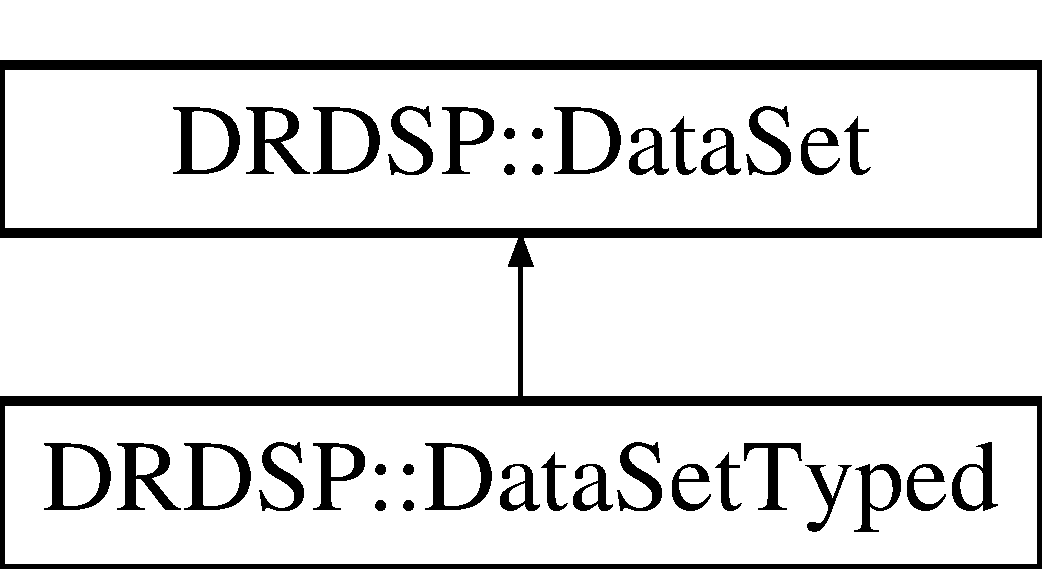
\includegraphics[height=2.000000cm]{struct_d_r_d_s_p_1_1_data_set}
\end{center}
\end{figure}
\subsection*{Public Member Functions}
\begin{DoxyCompactItemize}
\item 
\hypertarget{struct_d_r_d_s_p_1_1_data_set_ab1fec22ab532a161837090408b0cfd8c}{{\bfseries Data\-Set} (size\-\_\-t num\-Points, uint32\-\_\-t dim)}\label{struct_d_r_d_s_p_1_1_data_set_ab1fec22ab532a161837090408b0cfd8c}

\item 
\hypertarget{struct_d_r_d_s_p_1_1_data_set_a0ffb95866863d3b2bad35b0c68c6c7f3}{bool \hyperlink{struct_d_r_d_s_p_1_1_data_set_a0ffb95866863d3b2bad35b0c68c6c7f3}{Load\-Binary} (const char $\ast$filename)}\label{struct_d_r_d_s_p_1_1_data_set_a0ffb95866863d3b2bad35b0c68c6c7f3}

\begin{DoxyCompactList}\small\item\em Load a data set from file in binary format. \end{DoxyCompactList}\item 
\hypertarget{struct_d_r_d_s_p_1_1_data_set_a9caf2a2c685f1433028de6d3c11bd758}{bool \hyperlink{struct_d_r_d_s_p_1_1_data_set_a9caf2a2c685f1433028de6d3c11bd758}{Load\-Text} (const char $\ast$filename)}\label{struct_d_r_d_s_p_1_1_data_set_a9caf2a2c685f1433028de6d3c11bd758}

\begin{DoxyCompactList}\small\item\em Load a data set from file in text format (space separated) \end{DoxyCompactList}\item 
\hypertarget{struct_d_r_d_s_p_1_1_data_set_a1d90f86c1fbe0380d91158b1c050c501}{void \hyperlink{struct_d_r_d_s_p_1_1_data_set_a1d90f86c1fbe0380d91158b1c050c501}{Write\-C\-S\-V} (const char $\ast$filename) const }\label{struct_d_r_d_s_p_1_1_data_set_a1d90f86c1fbe0380d91158b1c050c501}

\begin{DoxyCompactList}\small\item\em Write the data set to file in C\-S\-V format. \end{DoxyCompactList}\item 
\hypertarget{struct_d_r_d_s_p_1_1_data_set_a0f42640d4f826807b69830bf3617152c}{\hyperlink{struct_d_r_d_s_p_1_1_data_set}{Data\-Set} \hyperlink{struct_d_r_d_s_p_1_1_data_set_a0f42640d4f826807b69830bf3617152c}{Project\-Data} (const Matrix\-Xd \&W) const }\label{struct_d_r_d_s_p_1_1_data_set_a0f42640d4f826807b69830bf3617152c}

\begin{DoxyCompactList}\small\item\em Apply the given projection to this data set. \end{DoxyCompactList}\item 
\hypertarget{struct_d_r_d_s_p_1_1_data_set_a6124959ad62a522b65cf6ad715166354}{Vector\-Xd \& {\bfseries operator\mbox{[}$\,$\mbox{]}} (size\-\_\-t i)}\label{struct_d_r_d_s_p_1_1_data_set_a6124959ad62a522b65cf6ad715166354}

\item 
\hypertarget{struct_d_r_d_s_p_1_1_data_set_aea3071fb03508e07e4d39056247eaaf9}{const Vector\-Xd \& {\bfseries operator\mbox{[}$\,$\mbox{]}} (size\-\_\-t i) const }\label{struct_d_r_d_s_p_1_1_data_set_aea3071fb03508e07e4d39056247eaaf9}

\end{DoxyCompactItemize}
\subsection*{Public Attributes}
\begin{DoxyCompactItemize}
\item 
\hypertarget{struct_d_r_d_s_p_1_1_data_set_aa2598262725329c137e03b8947638780}{uint32\-\_\-t \hyperlink{struct_d_r_d_s_p_1_1_data_set_aa2598262725329c137e03b8947638780}{dimension}}\label{struct_d_r_d_s_p_1_1_data_set_aa2598262725329c137e03b8947638780}

\begin{DoxyCompactList}\small\item\em Dimension of the space. \end{DoxyCompactList}\item 
\hypertarget{struct_d_r_d_s_p_1_1_data_set_ac486c907dea215957d503dc4dc9d76e3}{vector$<$ Vector\-Xd $>$ \hyperlink{struct_d_r_d_s_p_1_1_data_set_ac486c907dea215957d503dc4dc9d76e3}{points}}\label{struct_d_r_d_s_p_1_1_data_set_ac486c907dea215957d503dc4dc9d76e3}

\begin{DoxyCompactList}\small\item\em Array of data vectors. \end{DoxyCompactList}\end{DoxyCompactItemize}


\subsection{Detailed Description}
A set of data points. 

The documentation for this struct was generated from the following files\-:\begin{DoxyCompactItemize}
\item 
include/\-D\-R\-D\-S\-P/data/data\-\_\-set.\-h\item 
src/data/data\-\_\-set.\-cpp\end{DoxyCompactItemize}

\hypertarget{struct_d_r_d_s_p_1_1_data_set_typed}{\section{D\-R\-D\-S\-P\-:\-:Data\-Set\-Typed Struct Reference}
\label{struct_d_r_d_s_p_1_1_data_set_typed}\index{D\-R\-D\-S\-P\-::\-Data\-Set\-Typed@{D\-R\-D\-S\-P\-::\-Data\-Set\-Typed}}
}
Inheritance diagram for D\-R\-D\-S\-P\-:\-:Data\-Set\-Typed\-:\begin{figure}[H]
\begin{center}
\leavevmode
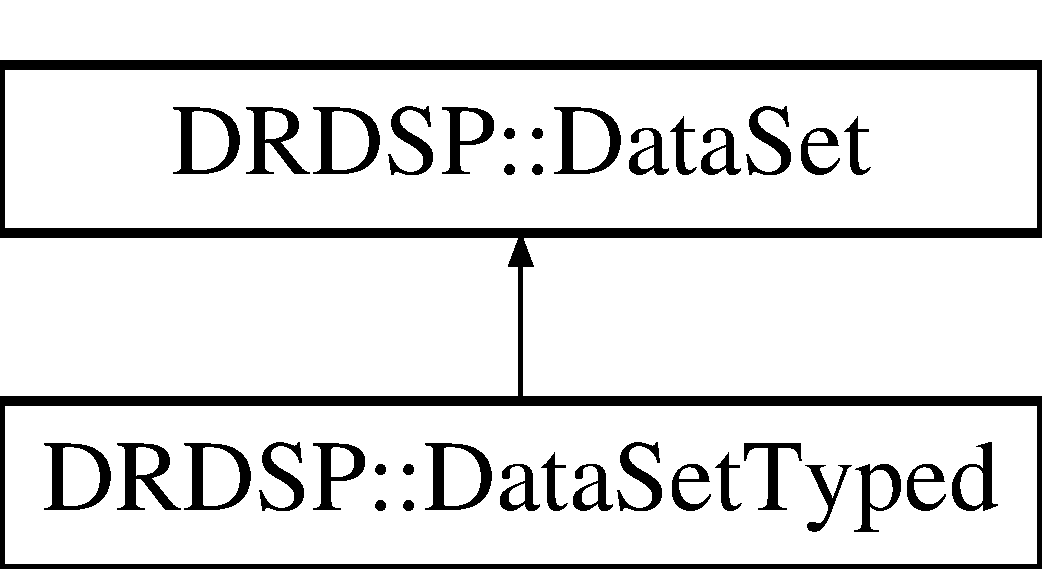
\includegraphics[height=2.000000cm]{struct_d_r_d_s_p_1_1_data_set_typed}
\end{center}
\end{figure}
\subsection*{Public Member Functions}
\begin{DoxyCompactItemize}
\item 
\hypertarget{struct_d_r_d_s_p_1_1_data_set_typed_acb54ebaf165fd365edc9adaa05c9ae44}{{\bfseries Data\-Set\-Typed} (const \hyperlink{struct_d_r_d_s_p_1_1_data_set_typed}{Data\-Set\-Typed} \&rhs)}\label{struct_d_r_d_s_p_1_1_data_set_typed_acb54ebaf165fd365edc9adaa05c9ae44}

\item 
\hypertarget{struct_d_r_d_s_p_1_1_data_set_typed_a87f023734d2ace299859cfcc685c7797}{{\bfseries Data\-Set\-Typed} (const \hyperlink{struct_d_r_d_s_p_1_1_data_set_typed}{Data\-Set\-Typed} \&\&rhs)}\label{struct_d_r_d_s_p_1_1_data_set_typed_a87f023734d2ace299859cfcc685c7797}

\item 
\hypertarget{struct_d_r_d_s_p_1_1_data_set_typed_a57f2f8449d2390b76aa98de3dbde73ca}{void {\bfseries Create} (uint32\-\_\-t num\-Points, uint32\-\_\-t dim)}\label{struct_d_r_d_s_p_1_1_data_set_typed_a57f2f8449d2390b76aa98de3dbde73ca}

\item 
\hypertarget{struct_d_r_d_s_p_1_1_data_set_typed_ae6876dff24b83610eaed933ff2c5d8e4}{void {\bfseries Destroy} ()}\label{struct_d_r_d_s_p_1_1_data_set_typed_ae6876dff24b83610eaed933ff2c5d8e4}

\end{DoxyCompactItemize}
\subsection*{Public Attributes}
\begin{DoxyCompactItemize}
\item 
\hypertarget{struct_d_r_d_s_p_1_1_data_set_typed_aa1d334ce3351a184e8234276b29d091e}{uint16\-\_\-t $\ast$ {\bfseries types}}\label{struct_d_r_d_s_p_1_1_data_set_typed_aa1d334ce3351a184e8234276b29d091e}

\end{DoxyCompactItemize}


The documentation for this struct was generated from the following files\-:\begin{DoxyCompactItemize}
\item 
include/\-D\-R\-D\-S\-P/data/data\-\_\-typed.\-h\item 
src/data/data\-\_\-typed.\-cpp\end{DoxyCompactItemize}

\hypertarget{struct_d_r_d_s_p_1_1_data_system}{\section{D\-R\-D\-S\-P\-:\-:Data\-System Struct Reference}
\label{struct_d_r_d_s_p_1_1_data_system}\index{D\-R\-D\-S\-P\-::\-Data\-System@{D\-R\-D\-S\-P\-::\-Data\-System}}
}


A family of data sets with corresponding parameter values.  




{\ttfamily \#include $<$data\-\_\-system.\-h$>$}

\subsection*{Public Member Functions}
\begin{DoxyCompactItemize}
\item 
\hypertarget{struct_d_r_d_s_p_1_1_data_system_aff122ec613cf26452c910ae884b11095}{{\bfseries Data\-System} (uint32\-\_\-t dim, uint32\-\_\-t num\-Params, uint32\-\_\-t param\-Dim)}\label{struct_d_r_d_s_p_1_1_data_system_aff122ec613cf26452c910ae884b11095}

\item 
\hypertarget{struct_d_r_d_s_p_1_1_data_system_a23b905c286750d16f9cd8996ad4c2076}{bool \hyperlink{struct_d_r_d_s_p_1_1_data_system_a23b905c286750d16f9cd8996ad4c2076}{Load} (const char $\ast$filename, uint32\-\_\-t max\-Points=0)}\label{struct_d_r_d_s_p_1_1_data_system_a23b905c286750d16f9cd8996ad4c2076}

\begin{DoxyCompactList}\small\item\em Load a data system from a text file. \end{DoxyCompactList}\item 
\hypertarget{struct_d_r_d_s_p_1_1_data_system_a1c2765c2e9a5b228dfd5c7487d67f94b}{bool \hyperlink{struct_d_r_d_s_p_1_1_data_system_a1c2765c2e9a5b228dfd5c7487d67f94b}{Load\-Set\-Binary} (const char $\ast$filename, uint32\-\_\-t i, uint32\-\_\-t max\-Points=0)}\label{struct_d_r_d_s_p_1_1_data_system_a1c2765c2e9a5b228dfd5c7487d67f94b}

\begin{DoxyCompactList}\small\item\em Load the ith data set from the given file in binary format. \end{DoxyCompactList}\item 
\hypertarget{struct_d_r_d_s_p_1_1_data_system_acf1c420d18c840b32fa5891f03253ee4}{bool \hyperlink{struct_d_r_d_s_p_1_1_data_system_acf1c420d18c840b32fa5891f03253ee4}{Load\-Set\-Text} (const char $\ast$filename, uint32\-\_\-t i, uint32\-\_\-t max\-Points=0)}\label{struct_d_r_d_s_p_1_1_data_system_acf1c420d18c840b32fa5891f03253ee4}

\begin{DoxyCompactList}\small\item\em Load the ith data set from the given file in text format (space separated) \end{DoxyCompactList}\item 
\hypertarget{struct_d_r_d_s_p_1_1_data_system_a6b4e0e6bc3ba1135a08fc2c2ed874e39}{void \hyperlink{struct_d_r_d_s_p_1_1_data_system_a6b4e0e6bc3ba1135a08fc2c2ed874e39}{Write\-Data\-Sets\-C\-S\-V} (const char $\ast$file\-Prefix, const char $\ast$file\-Suffix) const }\label{struct_d_r_d_s_p_1_1_data_system_a6b4e0e6bc3ba1135a08fc2c2ed874e39}

\begin{DoxyCompactList}\small\item\em Write the data sets to numbered files with given prefix and suffix. \end{DoxyCompactList}\item 
\hypertarget{struct_d_r_d_s_p_1_1_data_system_afd5e714d21c0d7c1b1efb65b233788ab}{\hyperlink{struct_d_r_d_s_p_1_1_data_system}{Data\-System} \hyperlink{struct_d_r_d_s_p_1_1_data_system_afd5e714d21c0d7c1b1efb65b233788ab}{Project\-Data} (const Matrix\-Xd \&W) const }\label{struct_d_r_d_s_p_1_1_data_system_afd5e714d21c0d7c1b1efb65b233788ab}

\begin{DoxyCompactList}\small\item\em Apply the given projection to this data system. \end{DoxyCompactList}\end{DoxyCompactItemize}
\subsection*{Public Attributes}
\begin{DoxyCompactItemize}
\item 
\hypertarget{struct_d_r_d_s_p_1_1_data_system_ab6aefaa08cd0a5b6a9e83105ecd56289}{uint32\-\_\-t \hyperlink{struct_d_r_d_s_p_1_1_data_system_ab6aefaa08cd0a5b6a9e83105ecd56289}{dimension}}\label{struct_d_r_d_s_p_1_1_data_system_ab6aefaa08cd0a5b6a9e83105ecd56289}

\begin{DoxyCompactList}\small\item\em Dimension of the space in which the data points live. \end{DoxyCompactList}\item 
\hypertarget{struct_d_r_d_s_p_1_1_data_system_a621ef4f4452821030bb57e93dadf334e}{uint32\-\_\-t \hyperlink{struct_d_r_d_s_p_1_1_data_system_a621ef4f4452821030bb57e93dadf334e}{num\-Parameters}}\label{struct_d_r_d_s_p_1_1_data_system_a621ef4f4452821030bb57e93dadf334e}

\begin{DoxyCompactList}\small\item\em Number of parameters/data sets in the family. \end{DoxyCompactList}\item 
\hypertarget{struct_d_r_d_s_p_1_1_data_system_ac494c5833ae14e805cd1d0a8b8e52143}{uint32\-\_\-t \hyperlink{struct_d_r_d_s_p_1_1_data_system_ac494c5833ae14e805cd1d0a8b8e52143}{parameter\-Dimension}}\label{struct_d_r_d_s_p_1_1_data_system_ac494c5833ae14e805cd1d0a8b8e52143}

\begin{DoxyCompactList}\small\item\em Dimension of the parameter space. \end{DoxyCompactList}\item 
\hypertarget{struct_d_r_d_s_p_1_1_data_system_a5fe0b41909f9056f986b4284e0fcb614}{vector$<$ \hyperlink{struct_d_r_d_s_p_1_1_data_set}{Data\-Set} $>$ \hyperlink{struct_d_r_d_s_p_1_1_data_system_a5fe0b41909f9056f986b4284e0fcb614}{data\-Sets}}\label{struct_d_r_d_s_p_1_1_data_system_a5fe0b41909f9056f986b4284e0fcb614}

\begin{DoxyCompactList}\small\item\em Array of data sets. \end{DoxyCompactList}\item 
\hypertarget{struct_d_r_d_s_p_1_1_data_system_aae14ac3e8c2e1a397759cd3a4d8a102f}{vector$<$ Vector\-Xd $>$ \hyperlink{struct_d_r_d_s_p_1_1_data_system_aae14ac3e8c2e1a397759cd3a4d8a102f}{parameters}}\label{struct_d_r_d_s_p_1_1_data_system_aae14ac3e8c2e1a397759cd3a4d8a102f}

\begin{DoxyCompactList}\small\item\em Array of parameter values. \end{DoxyCompactList}\end{DoxyCompactItemize}


\subsection{Detailed Description}
A family of data sets with corresponding parameter values. 

The documentation for this struct was generated from the following files\-:\begin{DoxyCompactItemize}
\item 
include/\-D\-R\-D\-S\-P/data/data\-\_\-system.\-h\item 
src/data/data\-\_\-system.\-cpp\end{DoxyCompactItemize}

\hypertarget{struct_d_r_d_s_p_1_1_data_system_typed}{\section{D\-R\-D\-S\-P\-:\-:Data\-System\-Typed Struct Reference}
\label{struct_d_r_d_s_p_1_1_data_system_typed}\index{D\-R\-D\-S\-P\-::\-Data\-System\-Typed@{D\-R\-D\-S\-P\-::\-Data\-System\-Typed}}
}
\subsection*{Public Member Functions}
\begin{DoxyCompactItemize}
\item 
\hypertarget{struct_d_r_d_s_p_1_1_data_system_typed_aeca993ba97569b6cce26575df8fd71a2}{{\bfseries Data\-System\-Typed} (const \hyperlink{struct_d_r_d_s_p_1_1_data_system_typed}{Data\-System\-Typed} \&rhs)}\label{struct_d_r_d_s_p_1_1_data_system_typed_aeca993ba97569b6cce26575df8fd71a2}

\item 
\hypertarget{struct_d_r_d_s_p_1_1_data_system_typed_a36dcf2bd60c1e177507d1215ab8baf57}{{\bfseries Data\-System\-Typed} (const \hyperlink{struct_d_r_d_s_p_1_1_data_system_typed}{Data\-System\-Typed} \&\&rhs)}\label{struct_d_r_d_s_p_1_1_data_system_typed_a36dcf2bd60c1e177507d1215ab8baf57}

\item 
\hypertarget{struct_d_r_d_s_p_1_1_data_system_typed_acc04596b19fc88c69fcf404573e6dc3a}{void {\bfseries Create} (uint32\-\_\-t dim, uint16\-\_\-t num\-Params, uint8\-\_\-t param\-Dim)}\label{struct_d_r_d_s_p_1_1_data_system_typed_acc04596b19fc88c69fcf404573e6dc3a}

\item 
\hypertarget{struct_d_r_d_s_p_1_1_data_system_typed_a0ebf2395136854994f8dbc876b27ef16}{void {\bfseries Destroy} ()}\label{struct_d_r_d_s_p_1_1_data_system_typed_a0ebf2395136854994f8dbc876b27ef16}

\item 
\hypertarget{struct_d_r_d_s_p_1_1_data_system_typed_a98e789d6a53c5d8e0b78b53421d24164}{bool {\bfseries Load} (const char $\ast$filename)}\label{struct_d_r_d_s_p_1_1_data_system_typed_a98e789d6a53c5d8e0b78b53421d24164}

\item 
\hypertarget{struct_d_r_d_s_p_1_1_data_system_typed_a771a4fb04c009cab7a220aea627b68b3}{bool {\bfseries Load\-Set\-Binary} (const char $\ast$filename, uint32\-\_\-t i)}\label{struct_d_r_d_s_p_1_1_data_system_typed_a771a4fb04c009cab7a220aea627b68b3}

\item 
\hypertarget{struct_d_r_d_s_p_1_1_data_system_typed_a7a895514d71f542392931a54125bc69a}{bool {\bfseries Load\-Set\-Text} (const char $\ast$filename, uint32\-\_\-t i)}\label{struct_d_r_d_s_p_1_1_data_system_typed_a7a895514d71f542392931a54125bc69a}

\end{DoxyCompactItemize}
\subsection*{Public Attributes}
\begin{DoxyCompactItemize}
\item 
\hypertarget{struct_d_r_d_s_p_1_1_data_system_typed_a19267fafd70c07c177b9992468704504}{\hyperlink{struct_d_r_d_s_p_1_1_data_set_typed}{Data\-Set\-Typed} $\ast$ {\bfseries data\-Sets}}\label{struct_d_r_d_s_p_1_1_data_system_typed_a19267fafd70c07c177b9992468704504}

\item 
\hypertarget{struct_d_r_d_s_p_1_1_data_system_typed_a14e96a1e32444f7a799e3d5552317aa5}{Vector\-Xd $\ast$ {\bfseries parameters}}\label{struct_d_r_d_s_p_1_1_data_system_typed_a14e96a1e32444f7a799e3d5552317aa5}

\item 
\hypertarget{struct_d_r_d_s_p_1_1_data_system_typed_a2b4eaddeb36714703850fdb92050ca0a}{uint32\-\_\-t {\bfseries dimension}}\label{struct_d_r_d_s_p_1_1_data_system_typed_a2b4eaddeb36714703850fdb92050ca0a}

\item 
\hypertarget{struct_d_r_d_s_p_1_1_data_system_typed_a02ab7e32e3df6e667e176144520c339c}{uint32\-\_\-t {\bfseries max\-Points}}\label{struct_d_r_d_s_p_1_1_data_system_typed_a02ab7e32e3df6e667e176144520c339c}

\item 
\hypertarget{struct_d_r_d_s_p_1_1_data_system_typed_a965e1066f9c4449413add3978a4cb0af}{uint16\-\_\-t {\bfseries num\-Parameters}}\label{struct_d_r_d_s_p_1_1_data_system_typed_a965e1066f9c4449413add3978a4cb0af}

\item 
\hypertarget{struct_d_r_d_s_p_1_1_data_system_typed_af3b60c8a97dc029652d551b7cdd34be4}{uint8\-\_\-t {\bfseries parameter\-Dimension}}\label{struct_d_r_d_s_p_1_1_data_system_typed_af3b60c8a97dc029652d551b7cdd34be4}

\item 
\hypertarget{struct_d_r_d_s_p_1_1_data_system_typed_ae8a12c2b02ef3ddb0bf370a2461a2201}{bool {\bfseries binary}}\label{struct_d_r_d_s_p_1_1_data_system_typed_ae8a12c2b02ef3ddb0bf370a2461a2201}

\end{DoxyCompactItemize}


The documentation for this struct was generated from the following files\-:\begin{DoxyCompactItemize}
\item 
include/\-D\-R\-D\-S\-P/data/data\-\_\-typed.\-h\item 
src/data/data\-\_\-typed.\-cpp\end{DoxyCompactItemize}

\hypertarget{struct_d_r_d_s_p_1_1_degrees}{\section{D\-R\-D\-S\-P\-:\-:Degrees$<$ T $>$ Struct Template Reference}
\label{struct_d_r_d_s_p_1_1_degrees}\index{D\-R\-D\-S\-P\-::\-Degrees$<$ T $>$@{D\-R\-D\-S\-P\-::\-Degrees$<$ T $>$}}
}
\subsection*{Public Member Functions}
\begin{DoxyCompactItemize}
\item 
\hypertarget{struct_d_r_d_s_p_1_1_degrees_aea5edb6561a07718684dabe4db75023a}{{\bfseries Degrees} (T rhs)}\label{struct_d_r_d_s_p_1_1_degrees_aea5edb6561a07718684dabe4db75023a}

\item 
\hypertarget{struct_d_r_d_s_p_1_1_degrees_a0d9d008f3a956963c5948ef48804f4bd}{{\bfseries Degrees} (const \hyperlink{struct_d_r_d_s_p_1_1_radians}{Radians}$<$ T $>$ \&rhs)}\label{struct_d_r_d_s_p_1_1_degrees_a0d9d008f3a956963c5948ef48804f4bd}

\item 
\hypertarget{struct_d_r_d_s_p_1_1_degrees_ac3bcd16cbcc7506b8a106137886517bc}{\hyperlink{struct_d_r_d_s_p_1_1_degrees}{Degrees}$<$ T $>$ \& {\bfseries operator=} (const \hyperlink{struct_d_r_d_s_p_1_1_radians}{Radians}$<$ T $>$ \&rhs)}\label{struct_d_r_d_s_p_1_1_degrees_ac3bcd16cbcc7506b8a106137886517bc}

\item 
\hypertarget{struct_d_r_d_s_p_1_1_degrees_a1f39a39d2d074f689b011a7cf19913d8}{\hyperlink{struct_d_r_d_s_p_1_1_degrees}{Degrees}$<$ T $>$ {\bfseries operator+} (const \hyperlink{struct_d_r_d_s_p_1_1_degrees}{Degrees}$<$ T $>$ \&rhs) const }\label{struct_d_r_d_s_p_1_1_degrees_a1f39a39d2d074f689b011a7cf19913d8}

\item 
\hypertarget{struct_d_r_d_s_p_1_1_degrees_ab1ffcb0e94295f81b13593291984b942}{\hyperlink{struct_d_r_d_s_p_1_1_degrees}{Degrees}$<$ T $>$ {\bfseries operator-\/} (const \hyperlink{struct_d_r_d_s_p_1_1_degrees}{Degrees}$<$ T $>$ \&rhs) const }\label{struct_d_r_d_s_p_1_1_degrees_ab1ffcb0e94295f81b13593291984b942}

\item 
\hypertarget{struct_d_r_d_s_p_1_1_degrees_af1390b65c4786bc138f20a28a29b94c4}{\hyperlink{struct_d_r_d_s_p_1_1_degrees}{Degrees}$<$ T $>$ {\bfseries operator$\ast$} (T x) const }\label{struct_d_r_d_s_p_1_1_degrees_af1390b65c4786bc138f20a28a29b94c4}

\item 
\hypertarget{struct_d_r_d_s_p_1_1_degrees_a988b52b56bf17ea5676b2584bd808532}{\hyperlink{struct_d_r_d_s_p_1_1_degrees}{Degrees}$<$ T $>$ {\bfseries operator/} (T x) const }\label{struct_d_r_d_s_p_1_1_degrees_a988b52b56bf17ea5676b2584bd808532}

\item 
\hypertarget{struct_d_r_d_s_p_1_1_degrees_aa4feef45aa496d9dc4b64612ed3fcd06}{\hyperlink{struct_d_r_d_s_p_1_1_degrees}{Degrees}$<$ T $>$ \& {\bfseries operator+=} (const \hyperlink{struct_d_r_d_s_p_1_1_degrees}{Degrees}$<$ T $>$ \&rhs)}\label{struct_d_r_d_s_p_1_1_degrees_aa4feef45aa496d9dc4b64612ed3fcd06}

\item 
\hypertarget{struct_d_r_d_s_p_1_1_degrees_aec831bd12465f0318ba18ed43ca61a3b}{\hyperlink{struct_d_r_d_s_p_1_1_degrees}{Degrees}$<$ T $>$ \& {\bfseries operator-\/=} (const \hyperlink{struct_d_r_d_s_p_1_1_degrees}{Degrees}$<$ T $>$ \&rhs)}\label{struct_d_r_d_s_p_1_1_degrees_aec831bd12465f0318ba18ed43ca61a3b}

\item 
\hypertarget{struct_d_r_d_s_p_1_1_degrees_ab263b47af616996e14eb97fda5805791}{\hyperlink{struct_d_r_d_s_p_1_1_degrees}{Degrees}$<$ T $>$ \& {\bfseries operator$\ast$=} (T x)}\label{struct_d_r_d_s_p_1_1_degrees_ab263b47af616996e14eb97fda5805791}

\item 
\hypertarget{struct_d_r_d_s_p_1_1_degrees_aa6ea9f7da8d6cb527c6a565449e07378}{\hyperlink{struct_d_r_d_s_p_1_1_degrees}{Degrees}$<$ T $>$ \& {\bfseries operator/=} (T x)}\label{struct_d_r_d_s_p_1_1_degrees_aa6ea9f7da8d6cb527c6a565449e07378}

\item 
\hypertarget{struct_d_r_d_s_p_1_1_degrees_a5e19aa3c231ee3ae31fddc109b8c913c}{\hyperlink{struct_d_r_d_s_p_1_1_degrees}{Degrees}$<$ T $>$ {\bfseries operator-\/} () const }\label{struct_d_r_d_s_p_1_1_degrees_a5e19aa3c231ee3ae31fddc109b8c913c}

\item 
\hypertarget{struct_d_r_d_s_p_1_1_degrees_a2f44722460deba00a72caae7b275cec3}{bool {\bfseries operator$>$} (const \hyperlink{struct_d_r_d_s_p_1_1_degrees}{Degrees}$<$ T $>$ \&rhs) const }\label{struct_d_r_d_s_p_1_1_degrees_a2f44722460deba00a72caae7b275cec3}

\item 
\hypertarget{struct_d_r_d_s_p_1_1_degrees_a7b2efa68737b7f423ff8e23c23fdad7a}{bool {\bfseries operator$<$} (const \hyperlink{struct_d_r_d_s_p_1_1_degrees}{Degrees}$<$ T $>$ \&rhs) const }\label{struct_d_r_d_s_p_1_1_degrees_a7b2efa68737b7f423ff8e23c23fdad7a}

\item 
\hypertarget{struct_d_r_d_s_p_1_1_degrees_a4418a174bf12974fc9099c289342ade1}{bool {\bfseries operator$>$=} (const \hyperlink{struct_d_r_d_s_p_1_1_degrees}{Degrees}$<$ T $>$ \&rhs) const }\label{struct_d_r_d_s_p_1_1_degrees_a4418a174bf12974fc9099c289342ade1}

\item 
\hypertarget{struct_d_r_d_s_p_1_1_degrees_a0182f3a600110193a691531aa6eafc3a}{bool {\bfseries operator$<$=} (const \hyperlink{struct_d_r_d_s_p_1_1_degrees}{Degrees}$<$ T $>$ \&rhs) const }\label{struct_d_r_d_s_p_1_1_degrees_a0182f3a600110193a691531aa6eafc3a}

\item 
\hypertarget{struct_d_r_d_s_p_1_1_degrees_a31d8be6980818e2a58f095aa7ebfc439}{{\bfseries operator T} () const }\label{struct_d_r_d_s_p_1_1_degrees_a31d8be6980818e2a58f095aa7ebfc439}

\end{DoxyCompactItemize}
\subsection*{Public Attributes}
\begin{DoxyCompactItemize}
\item 
\hypertarget{struct_d_r_d_s_p_1_1_degrees_a899380ba73155ddf4456cdd44e4088f7}{T {\bfseries value}}\label{struct_d_r_d_s_p_1_1_degrees_a899380ba73155ddf4456cdd44e4088f7}

\end{DoxyCompactItemize}


The documentation for this struct was generated from the following file\-:\begin{DoxyCompactItemize}
\item 
include/\-D\-R\-D\-S\-P/geometry/angle.\-h\end{DoxyCompactItemize}

\hypertarget{struct_d_r_d_s_p_1_1_discrete_dynamical_system}{\section{D\-R\-D\-S\-P\-:\-:Discrete\-Dynamical\-System$<$ State, Map $>$ Struct Template Reference}
\label{struct_d_r_d_s_p_1_1_discrete_dynamical_system}\index{D\-R\-D\-S\-P\-::\-Discrete\-Dynamical\-System$<$ State, Map $>$@{D\-R\-D\-S\-P\-::\-Discrete\-Dynamical\-System$<$ State, Map $>$}}
}
\subsection*{Public Member Functions}
\begin{DoxyCompactItemize}
\item 
\hypertarget{struct_d_r_d_s_p_1_1_discrete_dynamical_system_ad3f73c7a93a088ec169a7c351805abe0}{{\bfseries Discrete\-Dynamical\-System} (const Map \&map)}\label{struct_d_r_d_s_p_1_1_discrete_dynamical_system_ad3f73c7a93a088ec169a7c351805abe0}

\item 
\hypertarget{struct_d_r_d_s_p_1_1_discrete_dynamical_system_a1c0ca0d2f4e25c0f28835141dd1e748f}{{\bfseries Discrete\-Dynamical\-System} (const State \&state)}\label{struct_d_r_d_s_p_1_1_discrete_dynamical_system_a1c0ca0d2f4e25c0f28835141dd1e748f}

\item 
\hypertarget{struct_d_r_d_s_p_1_1_discrete_dynamical_system_afcaaef52db0707cd40b81c23c433d962}{{\bfseries Discrete\-Dynamical\-System} (const Map \&map, const State \&state)}\label{struct_d_r_d_s_p_1_1_discrete_dynamical_system_afcaaef52db0707cd40b81c23c433d962}

\item 
\hypertarget{struct_d_r_d_s_p_1_1_discrete_dynamical_system_ac2e23c5da942cd1f4b484b95ae0075d0}{void {\bfseries Advance} (uint32\-\_\-t dt=1)}\label{struct_d_r_d_s_p_1_1_discrete_dynamical_system_ac2e23c5da942cd1f4b484b95ae0075d0}

\end{DoxyCompactItemize}
\subsection*{Public Attributes}
\begin{DoxyCompactItemize}
\item 
\hypertarget{struct_d_r_d_s_p_1_1_discrete_dynamical_system_a297828d4508bddd152b048cb895daf79}{State {\bfseries state}}\label{struct_d_r_d_s_p_1_1_discrete_dynamical_system_a297828d4508bddd152b048cb895daf79}

\item 
\hypertarget{struct_d_r_d_s_p_1_1_discrete_dynamical_system_ac2e502e92cbdac8d46010d5249ba9de6}{Map {\bfseries map}}\label{struct_d_r_d_s_p_1_1_discrete_dynamical_system_ac2e502e92cbdac8d46010d5249ba9de6}

\end{DoxyCompactItemize}


The documentation for this struct was generated from the following file\-:\begin{DoxyCompactItemize}
\item 
include/\-D\-R\-D\-S\-P/dynamics/dynamical\-System.\-h\end{DoxyCompactItemize}

\hypertarget{struct_d_r_d_s_p_1_1_dot_product}{\section{D\-R\-D\-S\-P\-:\-:Dot\-Product$<$ V $>$ Struct Template Reference}
\label{struct_d_r_d_s_p_1_1_dot_product}\index{D\-R\-D\-S\-P\-::\-Dot\-Product$<$ V $>$@{D\-R\-D\-S\-P\-::\-Dot\-Product$<$ V $>$}}
}
\subsection*{Public Types}
\begin{DoxyCompactItemize}
\item 
\hypertarget{struct_d_r_d_s_p_1_1_dot_product_a674690d8ab49b8908928fe2504c3f622}{typedef V {\bfseries Vector}}\label{struct_d_r_d_s_p_1_1_dot_product_a674690d8ab49b8908928fe2504c3f622}

\item 
\hypertarget{struct_d_r_d_s_p_1_1_dot_product_ac0a16f6680afea3bce145857073df6a4}{typedef \hyperlink{struct_d_r_d_s_p_1_1_traits}{Traits}$<$ V $>$\-::Scalar {\bfseries Scalar}}\label{struct_d_r_d_s_p_1_1_dot_product_ac0a16f6680afea3bce145857073df6a4}

\end{DoxyCompactItemize}
\subsection*{Public Member Functions}
\begin{DoxyCompactItemize}
\item 
\hypertarget{struct_d_r_d_s_p_1_1_dot_product_a7122ebb044ab606bc90eb87ce8cab3f7}{Scalar {\bfseries operator()} (const V \&x, const V \&y) const }\label{struct_d_r_d_s_p_1_1_dot_product_a7122ebb044ab606bc90eb87ce8cab3f7}

\item 
\hypertarget{struct_d_r_d_s_p_1_1_dot_product_a0fd7ddd85af95144a24b541ddd61c74e}{Scalar {\bfseries Norm2} (const V \&x) const }\label{struct_d_r_d_s_p_1_1_dot_product_a0fd7ddd85af95144a24b541ddd61c74e}

\end{DoxyCompactItemize}


The documentation for this struct was generated from the following file\-:\begin{DoxyCompactItemize}
\item 
include/\-D\-R\-D\-S\-P/geometry/metric.\-h\end{DoxyCompactItemize}

\hypertarget{struct_d_r_d_s_p_1_1dual}{\section{D\-R\-D\-S\-P\-:\-:dual$<$ T $>$ Struct Template Reference}
\label{struct_d_r_d_s_p_1_1dual}\index{D\-R\-D\-S\-P\-::dual$<$ T $>$@{D\-R\-D\-S\-P\-::dual$<$ T $>$}}
}
\subsection*{Public Member Functions}
\begin{DoxyCompactItemize}
\item 
\hypertarget{struct_d_r_d_s_p_1_1dual_a8169a404e5a23d3659ad64aaf277fb6f}{{\bfseries dual} (T real)}\label{struct_d_r_d_s_p_1_1dual_a8169a404e5a23d3659ad64aaf277fb6f}

\item 
\hypertarget{struct_d_r_d_s_p_1_1dual_a86ae3acecf82009679f1ea3c422728e9}{{\bfseries dual} (T real, T \hyperlink{struct_d_r_d_s_p_1_1dual}{dual})}\label{struct_d_r_d_s_p_1_1dual_a86ae3acecf82009679f1ea3c422728e9}

\item 
\hypertarget{struct_d_r_d_s_p_1_1dual_a269257910dad7487cfe6b7f695585d39}{\hyperlink{struct_d_r_d_s_p_1_1dual}{dual}$<$ T $>$ {\bfseries operator-\/} () const }\label{struct_d_r_d_s_p_1_1dual_a269257910dad7487cfe6b7f695585d39}

\item 
\hypertarget{struct_d_r_d_s_p_1_1dual_ab18cda06a306a0bb97deabac1a8fd1ae}{\hyperlink{struct_d_r_d_s_p_1_1dual}{dual}$<$ T $>$ {\bfseries operator+} (const \hyperlink{struct_d_r_d_s_p_1_1dual}{dual}$<$ T $>$ \&rhs) const }\label{struct_d_r_d_s_p_1_1dual_ab18cda06a306a0bb97deabac1a8fd1ae}

\item 
\hypertarget{struct_d_r_d_s_p_1_1dual_a7f066ea6def9c0af3081a265543e402a}{\hyperlink{struct_d_r_d_s_p_1_1dual}{dual}$<$ T $>$ {\bfseries operator-\/} (const \hyperlink{struct_d_r_d_s_p_1_1dual}{dual}$<$ T $>$ \&rhs) const }\label{struct_d_r_d_s_p_1_1dual_a7f066ea6def9c0af3081a265543e402a}

\item 
\hypertarget{struct_d_r_d_s_p_1_1dual_a263a4cfe97ce6f8f272b28a9ad297c90}{\hyperlink{struct_d_r_d_s_p_1_1dual}{dual}$<$ T $>$ {\bfseries operator$\ast$} (const \hyperlink{struct_d_r_d_s_p_1_1dual}{dual}$<$ T $>$ \&rhs) const }\label{struct_d_r_d_s_p_1_1dual_a263a4cfe97ce6f8f272b28a9ad297c90}

\item 
\hypertarget{struct_d_r_d_s_p_1_1dual_ac838ce569f85fd920d587bfe22b4228c}{\hyperlink{struct_d_r_d_s_p_1_1dual}{dual}$<$ T $>$ {\bfseries operator/} (const \hyperlink{struct_d_r_d_s_p_1_1dual}{dual}$<$ T $>$ \&rhs) const }\label{struct_d_r_d_s_p_1_1dual_ac838ce569f85fd920d587bfe22b4228c}

\item 
\hypertarget{struct_d_r_d_s_p_1_1dual_af928d72c558bc5251f48e3a8ef43e499}{\hyperlink{struct_d_r_d_s_p_1_1dual}{dual}$<$ T $>$ \& {\bfseries operator+=} (const \hyperlink{struct_d_r_d_s_p_1_1dual}{dual}$<$ T $>$ \&rhs)}\label{struct_d_r_d_s_p_1_1dual_af928d72c558bc5251f48e3a8ef43e499}

\item 
\hypertarget{struct_d_r_d_s_p_1_1dual_aeea91211e526cfd1ff76dd99228045fa}{\hyperlink{struct_d_r_d_s_p_1_1dual}{dual}$<$ T $>$ \& {\bfseries operator-\/=} (const \hyperlink{struct_d_r_d_s_p_1_1dual}{dual}$<$ T $>$ \&rhs)}\label{struct_d_r_d_s_p_1_1dual_aeea91211e526cfd1ff76dd99228045fa}

\item 
\hypertarget{struct_d_r_d_s_p_1_1dual_a5bdcc4cd454cd6b3a775d0e3ac9de853}{\hyperlink{struct_d_r_d_s_p_1_1dual}{dual}$<$ T $>$ \& {\bfseries operator$\ast$=} (const \hyperlink{struct_d_r_d_s_p_1_1dual}{dual}$<$ T $>$ \&rhs)}\label{struct_d_r_d_s_p_1_1dual_a5bdcc4cd454cd6b3a775d0e3ac9de853}

\item 
\hypertarget{struct_d_r_d_s_p_1_1dual_a68be03e1a9a0ae79edbcb1b012b4567b}{\hyperlink{struct_d_r_d_s_p_1_1dual}{dual}$<$ T $>$ \& {\bfseries operator/=} (const \hyperlink{struct_d_r_d_s_p_1_1dual}{dual}$<$ T $>$ \&rhs)}\label{struct_d_r_d_s_p_1_1dual_a68be03e1a9a0ae79edbcb1b012b4567b}

\item 
\hypertarget{struct_d_r_d_s_p_1_1dual_ac694c41d16a43f1a563d03dfda4cd7de}{\hyperlink{struct_d_r_d_s_p_1_1dual}{dual}$<$ T $>$ \& {\bfseries operator=} (T rhs)}\label{struct_d_r_d_s_p_1_1dual_ac694c41d16a43f1a563d03dfda4cd7de}

\item 
\hypertarget{struct_d_r_d_s_p_1_1dual_a6ebef014f1f9a8286129e2ee4349bb94}{\hyperlink{struct_d_r_d_s_p_1_1dual}{dual}$<$ T $>$ {\bfseries operator$\ast$} (T a) const }\label{struct_d_r_d_s_p_1_1dual_a6ebef014f1f9a8286129e2ee4349bb94}

\item 
\hypertarget{struct_d_r_d_s_p_1_1dual_a3806b3efe14465534ae3f69931c1728f}{\hyperlink{struct_d_r_d_s_p_1_1dual}{dual}$<$ T $>$ \& {\bfseries operator$\ast$=} (T a)}\label{struct_d_r_d_s_p_1_1dual_a3806b3efe14465534ae3f69931c1728f}

\item 
\hypertarget{struct_d_r_d_s_p_1_1dual_aee0393d389be9cab632f122a268a620d}{\hyperlink{struct_d_r_d_s_p_1_1dual}{dual}$<$ T $>$ {\bfseries operator/} (T a) const }\label{struct_d_r_d_s_p_1_1dual_aee0393d389be9cab632f122a268a620d}

\item 
\hypertarget{struct_d_r_d_s_p_1_1dual_aeec246dcd6730e2e3e23f9c6c0ea4e78}{\hyperlink{struct_d_r_d_s_p_1_1dual}{dual}$<$ T $>$ \& {\bfseries operator/=} (T a)}\label{struct_d_r_d_s_p_1_1dual_aeec246dcd6730e2e3e23f9c6c0ea4e78}

\item 
\hypertarget{struct_d_r_d_s_p_1_1dual_a36d28afb644f5f27dd1299b3e5c4ca0c}{T {\bfseries real\-\_\-part} () const }\label{struct_d_r_d_s_p_1_1dual_a36d28afb644f5f27dd1299b3e5c4ca0c}

\item 
\hypertarget{struct_d_r_d_s_p_1_1dual_af1d6079aacb711e6e05924bd131ff0d7}{T {\bfseries dual\-\_\-part} () const }\label{struct_d_r_d_s_p_1_1dual_af1d6079aacb711e6e05924bd131ff0d7}

\end{DoxyCompactItemize}
\subsection*{Public Attributes}
\begin{DoxyCompactItemize}
\item 
\hypertarget{struct_d_r_d_s_p_1_1dual_aa10eb23e32f77dacdc868c9a1df38b69}{T {\bfseries x}}\label{struct_d_r_d_s_p_1_1dual_aa10eb23e32f77dacdc868c9a1df38b69}

\item 
\hypertarget{struct_d_r_d_s_p_1_1dual_acc5892de3194e38d4c504467cfaa9da7}{T {\bfseries y}}\label{struct_d_r_d_s_p_1_1dual_acc5892de3194e38d4c504467cfaa9da7}

\end{DoxyCompactItemize}


The documentation for this struct was generated from the following file\-:\begin{DoxyCompactItemize}
\item 
include/\-D\-R\-D\-S\-P/dual.\-h\end{DoxyCompactItemize}

\hypertarget{struct_d_r_d_s_p_1_1_embedding}{\section{D\-R\-D\-S\-P\-:\-:Embedding Struct Reference}
\label{struct_d_r_d_s_p_1_1_embedding}\index{D\-R\-D\-S\-P\-::\-Embedding@{D\-R\-D\-S\-P\-::\-Embedding}}
}
\subsection*{Public Member Functions}
\begin{DoxyCompactItemize}
\item 
\hypertarget{struct_d_r_d_s_p_1_1_embedding_a044e60ce685c03b1e31a080455a47a43}{{\bfseries Embedding} (uint32\-\_\-t orig\-Dim, uint32\-\_\-t embed\-Dim)}\label{struct_d_r_d_s_p_1_1_embedding_a044e60ce685c03b1e31a080455a47a43}

\item 
\hypertarget{struct_d_r_d_s_p_1_1_embedding_a128ada65c8aafc9348dafd8c89add0da}{virtual Vector\-Xd {\bfseries Evaluate} (const Vector\-Xd \&x) const }\label{struct_d_r_d_s_p_1_1_embedding_a128ada65c8aafc9348dafd8c89add0da}

\item 
\hypertarget{struct_d_r_d_s_p_1_1_embedding_a18d562ec89da43df7dd66b1b8b694e85}{virtual Matrix\-Xd {\bfseries Derivative} (const Vector\-Xd \&x) const }\label{struct_d_r_d_s_p_1_1_embedding_a18d562ec89da43df7dd66b1b8b694e85}

\item 
\hypertarget{struct_d_r_d_s_p_1_1_embedding_a010327f5b83006a24e466deabad5a852}{virtual Matrix\-Xd {\bfseries Derivative\-Adjoint} (const Vector\-Xd \&x) const }\label{struct_d_r_d_s_p_1_1_embedding_a010327f5b83006a24e466deabad5a852}

\item 
\hypertarget{struct_d_r_d_s_p_1_1_embedding_ae651c3ad18c8ad3dbbfea1577d7d395f}{virtual Matrix\-Xd {\bfseries Derivative2} (const Vector\-Xd \&x, uint32\-\_\-t i) const }\label{struct_d_r_d_s_p_1_1_embedding_ae651c3ad18c8ad3dbbfea1577d7d395f}

\item 
\hypertarget{struct_d_r_d_s_p_1_1_embedding_a5d28c64ee0aa19fb2481f16795b31765}{Matrix\-Xd {\bfseries Compute\-Induced\-Metric} (const Vector\-Xd \&x) const }\label{struct_d_r_d_s_p_1_1_embedding_a5d28c64ee0aa19fb2481f16795b31765}

\item 
\hypertarget{struct_d_r_d_s_p_1_1_embedding_a71acf702383901f9d4aa6fb198dc0892}{\hyperlink{struct_d_r_d_s_p_1_1_data_set}{Data\-Set} {\bfseries Embed\-Data} (const \hyperlink{struct_d_r_d_s_p_1_1_data_set}{Data\-Set} \&data) const }\label{struct_d_r_d_s_p_1_1_embedding_a71acf702383901f9d4aa6fb198dc0892}

\item 
\hypertarget{struct_d_r_d_s_p_1_1_embedding_abdf67b0ed050b58fc9a0943d604093ef}{\hyperlink{struct_d_r_d_s_p_1_1_data_system}{Data\-System} {\bfseries Embed\-Data} (const \hyperlink{struct_d_r_d_s_p_1_1_data_system}{Data\-System} \&data) const }\label{struct_d_r_d_s_p_1_1_embedding_abdf67b0ed050b58fc9a0943d604093ef}

\end{DoxyCompactItemize}
\subsection*{Public Attributes}
\begin{DoxyCompactItemize}
\item 
\hypertarget{struct_d_r_d_s_p_1_1_embedding_ac49e8aa042fbf2ee8e9fdc3d2b4f1c26}{uint32\-\_\-t {\bfseries o\-Dim}}\label{struct_d_r_d_s_p_1_1_embedding_ac49e8aa042fbf2ee8e9fdc3d2b4f1c26}

\item 
\hypertarget{struct_d_r_d_s_p_1_1_embedding_aa49b8deb5d403025ca5db3f483c015b2}{uint32\-\_\-t {\bfseries e\-Dim}}\label{struct_d_r_d_s_p_1_1_embedding_aa49b8deb5d403025ca5db3f483c015b2}

\end{DoxyCompactItemize}


The documentation for this struct was generated from the following files\-:\begin{DoxyCompactItemize}
\item 
include/\-D\-R\-D\-S\-P/dynamics/embedding.\-h\item 
src/dynamics/embedding.\-cpp\end{DoxyCompactItemize}

\hypertarget{struct_d_r_d_s_p_1_1_equi_r_b_f_cyclic}{\section{D\-R\-D\-S\-P\-:\-:Equi\-R\-B\-F\-Cyclic$<$ F, N $>$ Struct Template Reference}
\label{struct_d_r_d_s_p_1_1_equi_r_b_f_cyclic}\index{D\-R\-D\-S\-P\-::\-Equi\-R\-B\-F\-Cyclic$<$ F, N $>$@{D\-R\-D\-S\-P\-::\-Equi\-R\-B\-F\-Cyclic$<$ F, N $>$}}
}
\subsection*{Public Types}
\begin{DoxyCompactItemize}
\item 
\hypertarget{struct_d_r_d_s_p_1_1_equi_r_b_f_cyclic_a4e0cd623b4aa759873ee402f2a0990a6}{typedef F {\bfseries Radial\-Type}}\label{struct_d_r_d_s_p_1_1_equi_r_b_f_cyclic_a4e0cd623b4aa759873ee402f2a0990a6}

\end{DoxyCompactItemize}
\subsection*{Public Member Functions}
\begin{DoxyCompactItemize}
\item 
\hypertarget{struct_d_r_d_s_p_1_1_equi_r_b_f_cyclic_a800d640944e8c1656141faf6092da51b}{{\bfseries Equi\-R\-B\-F\-Cyclic} (const F \&f)}\label{struct_d_r_d_s_p_1_1_equi_r_b_f_cyclic_a800d640944e8c1656141faf6092da51b}

\item 
\hypertarget{struct_d_r_d_s_p_1_1_equi_r_b_f_cyclic_a0fc5d741bb0d61b57f77342ae92badca}{Vector\-Xd {\bfseries operator()} (const Vector\-Xd \&x) const }\label{struct_d_r_d_s_p_1_1_equi_r_b_f_cyclic_a0fc5d741bb0d61b57f77342ae92badca}

\item 
\hypertarget{struct_d_r_d_s_p_1_1_equi_r_b_f_cyclic_aa3d163e34f00f5bcf09dbd79d78b04fc}{Matrix\-Xd {\bfseries Derivative} (const Vector\-Xd \&x) const }\label{struct_d_r_d_s_p_1_1_equi_r_b_f_cyclic_aa3d163e34f00f5bcf09dbd79d78b04fc}

\item 
\hypertarget{struct_d_r_d_s_p_1_1_equi_r_b_f_cyclic_a2b869652866dfe11d89cea4d0e712e35}{Matrix\-Xd {\bfseries Linear\-Weight} (const Vector\-Xd \&x) const }\label{struct_d_r_d_s_p_1_1_equi_r_b_f_cyclic_a2b869652866dfe11d89cea4d0e712e35}

\item 
\hypertarget{struct_d_r_d_s_p_1_1_equi_r_b_f_cyclic_a5d2da45df91a08420e07c91ebdfca0b5}{Matrix\-Xd {\bfseries Linear\-Derivative\-Weight} (const Vector\-Xd \&x) const }\label{struct_d_r_d_s_p_1_1_equi_r_b_f_cyclic_a5d2da45df91a08420e07c91ebdfca0b5}

\end{DoxyCompactItemize}
\subsection*{Public Attributes}
\begin{DoxyCompactItemize}
\item 
\hypertarget{struct_d_r_d_s_p_1_1_equi_r_b_f_cyclic_a6152c13035f77c2978118d61e355ccf8}{Vector\-Xd {\bfseries weight}}\label{struct_d_r_d_s_p_1_1_equi_r_b_f_cyclic_a6152c13035f77c2978118d61e355ccf8}

\item 
\hypertarget{struct_d_r_d_s_p_1_1_equi_r_b_f_cyclic_a50bf2136d3c4d97c309a3895857a7bef}{Vector\-Xd {\bfseries centre}}\label{struct_d_r_d_s_p_1_1_equi_r_b_f_cyclic_a50bf2136d3c4d97c309a3895857a7bef}

\item 
\hypertarget{struct_d_r_d_s_p_1_1_equi_r_b_f_cyclic_aede00a915cd6434e393c2720520e087a}{Matrix\-Xd {\bfseries generator}}\label{struct_d_r_d_s_p_1_1_equi_r_b_f_cyclic_aede00a915cd6434e393c2720520e087a}

\item 
\hypertarget{struct_d_r_d_s_p_1_1_equi_r_b_f_cyclic_a639ef5af751e01e9a7c547d322be6b87}{F {\bfseries func}}\label{struct_d_r_d_s_p_1_1_equi_r_b_f_cyclic_a639ef5af751e01e9a7c547d322be6b87}

\end{DoxyCompactItemize}


The documentation for this struct was generated from the following file\-:\begin{DoxyCompactItemize}
\item 
include/\-D\-R\-D\-S\-P/dynamics/radial\-\_\-basis.\-h\end{DoxyCompactItemize}

\hypertarget{struct_d_r_d_s_p_1_1_equi_r_b_f_finite}{\section{D\-R\-D\-S\-P\-:\-:Equi\-R\-B\-F\-Finite$<$ F $>$ Struct Template Reference}
\label{struct_d_r_d_s_p_1_1_equi_r_b_f_finite}\index{D\-R\-D\-S\-P\-::\-Equi\-R\-B\-F\-Finite$<$ F $>$@{D\-R\-D\-S\-P\-::\-Equi\-R\-B\-F\-Finite$<$ F $>$}}
}
\subsection*{Public Types}
\begin{DoxyCompactItemize}
\item 
\hypertarget{struct_d_r_d_s_p_1_1_equi_r_b_f_finite_adb9b01f3272e7ac52fbd5b46c26880f2}{typedef F {\bfseries Radial\-Type}}\label{struct_d_r_d_s_p_1_1_equi_r_b_f_finite_adb9b01f3272e7ac52fbd5b46c26880f2}

\end{DoxyCompactItemize}
\subsection*{Public Member Functions}
\begin{DoxyCompactItemize}
\item 
\hypertarget{struct_d_r_d_s_p_1_1_equi_r_b_f_finite_a82e8171778b1d4fe07bd6b23e26c75ec}{{\bfseries Equi\-R\-B\-F\-Finite} (const F \&f)}\label{struct_d_r_d_s_p_1_1_equi_r_b_f_finite_a82e8171778b1d4fe07bd6b23e26c75ec}

\item 
\hypertarget{struct_d_r_d_s_p_1_1_equi_r_b_f_finite_a9d8ecdcfd2e198265584614aefda826d}{Vector\-Xd {\bfseries operator()} (const Vector\-Xd \&x) const }\label{struct_d_r_d_s_p_1_1_equi_r_b_f_finite_a9d8ecdcfd2e198265584614aefda826d}

\item 
\hypertarget{struct_d_r_d_s_p_1_1_equi_r_b_f_finite_ae535b16ca82be5e97f7e9336cea084fa}{Matrix\-Xd {\bfseries Derivative} (const Vector\-Xd \&x) const }\label{struct_d_r_d_s_p_1_1_equi_r_b_f_finite_ae535b16ca82be5e97f7e9336cea084fa}

\item 
\hypertarget{struct_d_r_d_s_p_1_1_equi_r_b_f_finite_a59f58eae316d14c2fffd53253f56fce2}{Matrix\-Xd {\bfseries Linear\-Weight} (const Vector\-Xd \&x) const }\label{struct_d_r_d_s_p_1_1_equi_r_b_f_finite_a59f58eae316d14c2fffd53253f56fce2}

\item 
\hypertarget{struct_d_r_d_s_p_1_1_equi_r_b_f_finite_adff6b2690e4a2399d437ec2a6e689664}{Matrix\-Xd {\bfseries Linear\-Derivative\-Weight} (const Vector\-Xd \&x) const }\label{struct_d_r_d_s_p_1_1_equi_r_b_f_finite_adff6b2690e4a2399d437ec2a6e689664}

\end{DoxyCompactItemize}
\subsection*{Public Attributes}
\begin{DoxyCompactItemize}
\item 
\hypertarget{struct_d_r_d_s_p_1_1_equi_r_b_f_finite_a34a57410440eb4963e166ffffd553dfc}{Vector\-Xd {\bfseries weight}}\label{struct_d_r_d_s_p_1_1_equi_r_b_f_finite_a34a57410440eb4963e166ffffd553dfc}

\item 
\hypertarget{struct_d_r_d_s_p_1_1_equi_r_b_f_finite_a486e079665ba3bf35822af822fd0ecec}{Vector\-Xd {\bfseries centre}}\label{struct_d_r_d_s_p_1_1_equi_r_b_f_finite_a486e079665ba3bf35822af822fd0ecec}

\item 
\hypertarget{struct_d_r_d_s_p_1_1_equi_r_b_f_finite_a9ccfe5aeb651a2793021eee7d4d93495}{vector$<$ Matrix\-Xd $>$ {\bfseries group}}\label{struct_d_r_d_s_p_1_1_equi_r_b_f_finite_a9ccfe5aeb651a2793021eee7d4d93495}

\item 
\hypertarget{struct_d_r_d_s_p_1_1_equi_r_b_f_finite_a3e0bea2200d1f16b930f4bd7d88292db}{F {\bfseries func}}\label{struct_d_r_d_s_p_1_1_equi_r_b_f_finite_a3e0bea2200d1f16b930f4bd7d88292db}

\end{DoxyCompactItemize}


The documentation for this struct was generated from the following file\-:\begin{DoxyCompactItemize}
\item 
include/\-D\-R\-D\-S\-P/dynamics/radial\-\_\-basis.\-h\end{DoxyCompactItemize}

\hypertarget{struct_d_r_d_s_p_1_1_equi_r_b_f_s_o2}{\section{D\-R\-D\-S\-P\-:\-:Equi\-R\-B\-F\-S\-O2$<$ F $>$ Struct Template Reference}
\label{struct_d_r_d_s_p_1_1_equi_r_b_f_s_o2}\index{D\-R\-D\-S\-P\-::\-Equi\-R\-B\-F\-S\-O2$<$ F $>$@{D\-R\-D\-S\-P\-::\-Equi\-R\-B\-F\-S\-O2$<$ F $>$}}
}


The documentation for this struct was generated from the following file\-:\begin{DoxyCompactItemize}
\item 
include/\-D\-R\-D\-S\-P/dynamics/radial\-\_\-basis.\-h\end{DoxyCompactItemize}

\hypertarget{struct_d_r_d_s_p_1_1_equi_r_b_f_s_o2_3_01_inverse_quadratic_01_4}{\section{D\-R\-D\-S\-P\-:\-:Equi\-R\-B\-F\-S\-O2$<$ Inverse\-Quadratic $>$ Struct Template Reference}
\label{struct_d_r_d_s_p_1_1_equi_r_b_f_s_o2_3_01_inverse_quadratic_01_4}\index{D\-R\-D\-S\-P\-::\-Equi\-R\-B\-F\-S\-O2$<$ Inverse\-Quadratic $>$@{D\-R\-D\-S\-P\-::\-Equi\-R\-B\-F\-S\-O2$<$ Inverse\-Quadratic $>$}}
}
\subsection*{Public Types}
\begin{DoxyCompactItemize}
\item 
\hypertarget{struct_d_r_d_s_p_1_1_equi_r_b_f_s_o2_3_01_inverse_quadratic_01_4_a10e12f81668783d7aea13cd71b999241}{typedef \hyperlink{struct_d_r_d_s_p_1_1_inverse_quadratic}{Inverse\-Quadratic} {\bfseries Radial\-Type}}\label{struct_d_r_d_s_p_1_1_equi_r_b_f_s_o2_3_01_inverse_quadratic_01_4_a10e12f81668783d7aea13cd71b999241}

\end{DoxyCompactItemize}
\subsection*{Public Member Functions}
\begin{DoxyCompactItemize}
\item 
\hypertarget{struct_d_r_d_s_p_1_1_equi_r_b_f_s_o2_3_01_inverse_quadratic_01_4_a515e457f292cf8e579f0ff68d47dbba1}{{\bfseries Equi\-R\-B\-F\-S\-O2} (const \hyperlink{struct_d_r_d_s_p_1_1_inverse_quadratic}{Inverse\-Quadratic} \&f)}\label{struct_d_r_d_s_p_1_1_equi_r_b_f_s_o2_3_01_inverse_quadratic_01_4_a515e457f292cf8e579f0ff68d47dbba1}

\item 
\hypertarget{struct_d_r_d_s_p_1_1_equi_r_b_f_s_o2_3_01_inverse_quadratic_01_4_a691663e6181d3ba09ec25235562015f8}{{\footnotesize template$<$typename Derived $>$ }\\Matrix$<$ typename \\*
Derived\-::\-Scalar,-\/1, 1 $>$ {\bfseries operator()} (const Matrix\-Base$<$ Derived $>$ \&x) const }\label{struct_d_r_d_s_p_1_1_equi_r_b_f_s_o2_3_01_inverse_quadratic_01_4_a691663e6181d3ba09ec25235562015f8}

\item 
\hypertarget{struct_d_r_d_s_p_1_1_equi_r_b_f_s_o2_3_01_inverse_quadratic_01_4_a5b0fc83d15864289fd58d6ac60deb635}{Matrix\-Xd {\bfseries Derivative} (const Vector\-Xd \&x) const }\label{struct_d_r_d_s_p_1_1_equi_r_b_f_s_o2_3_01_inverse_quadratic_01_4_a5b0fc83d15864289fd58d6ac60deb635}

\item 
\hypertarget{struct_d_r_d_s_p_1_1_equi_r_b_f_s_o2_3_01_inverse_quadratic_01_4_aced0ccd45028df75780a1ba776da9fc9}{Matrix\-Xd {\bfseries Linear\-Weight} (const Vector\-Xd \&x) const }\label{struct_d_r_d_s_p_1_1_equi_r_b_f_s_o2_3_01_inverse_quadratic_01_4_aced0ccd45028df75780a1ba776da9fc9}

\item 
\hypertarget{struct_d_r_d_s_p_1_1_equi_r_b_f_s_o2_3_01_inverse_quadratic_01_4_a1948467b9230ee7bce761028f4b0af06}{Matrix\-Xd {\bfseries Linear\-Derivative\-Weight} (const Vector\-Xd \&x) const }\label{struct_d_r_d_s_p_1_1_equi_r_b_f_s_o2_3_01_inverse_quadratic_01_4_a1948467b9230ee7bce761028f4b0af06}

\end{DoxyCompactItemize}
\subsection*{Public Attributes}
\begin{DoxyCompactItemize}
\item 
\hypertarget{struct_d_r_d_s_p_1_1_equi_r_b_f_s_o2_3_01_inverse_quadratic_01_4_aa214df28e0d7bfbc87251e424b9f649a}{Vector\-Xd {\bfseries weight}}\label{struct_d_r_d_s_p_1_1_equi_r_b_f_s_o2_3_01_inverse_quadratic_01_4_aa214df28e0d7bfbc87251e424b9f649a}

\item 
\hypertarget{struct_d_r_d_s_p_1_1_equi_r_b_f_s_o2_3_01_inverse_quadratic_01_4_ab729533d926eff8fe2e83db3326b3665}{Vector\-Xd {\bfseries centre}}\label{struct_d_r_d_s_p_1_1_equi_r_b_f_s_o2_3_01_inverse_quadratic_01_4_ab729533d926eff8fe2e83db3326b3665}

\item 
\hypertarget{struct_d_r_d_s_p_1_1_equi_r_b_f_s_o2_3_01_inverse_quadratic_01_4_a219626fd7be7c1273f6700ef099d3e74}{Matrix$<$ double,-\/1, 2 $>$ {\bfseries W}}\label{struct_d_r_d_s_p_1_1_equi_r_b_f_s_o2_3_01_inverse_quadratic_01_4_a219626fd7be7c1273f6700ef099d3e74}

\item 
\hypertarget{struct_d_r_d_s_p_1_1_equi_r_b_f_s_o2_3_01_inverse_quadratic_01_4_a176501afd75e5ee20dac8c33a709dcf1}{\hyperlink{struct_d_r_d_s_p_1_1_inverse_quadratic}{Inverse\-Quadratic} {\bfseries func}}\label{struct_d_r_d_s_p_1_1_equi_r_b_f_s_o2_3_01_inverse_quadratic_01_4_a176501afd75e5ee20dac8c33a709dcf1}

\end{DoxyCompactItemize}
\subsection*{Static Protected Member Functions}
\begin{DoxyCompactItemize}
\item 
\hypertarget{struct_d_r_d_s_p_1_1_equi_r_b_f_s_o2_3_01_inverse_quadratic_01_4_a690f78667c7e93ae1ef26c099f5be79f}{{\footnotesize template$<$typename Derived1 , typename Derived2 $>$ }\\static Matrix$<$ typename \\*
internal\-::scalar\-\_\-product\-\_\-traits\\*
$<$ typename Derived1\-::\-Scalar, \\*
typename Derived2\-::\-Scalar $>$\\*
\-::Return\-Type, 2, 2 $>$ {\bfseries Compute\-Rotation} (const Matrix\-Base$<$ Derived1 $>$ \&x, const Matrix\-Base$<$ Derived2 $>$ \&y)}\label{struct_d_r_d_s_p_1_1_equi_r_b_f_s_o2_3_01_inverse_quadratic_01_4_a690f78667c7e93ae1ef26c099f5be79f}

\end{DoxyCompactItemize}


The documentation for this struct was generated from the following file\-:\begin{DoxyCompactItemize}
\item 
include/\-D\-R\-D\-S\-P/dynamics/radial\-\_\-basis.\-h\end{DoxyCompactItemize}

\hypertarget{struct_d_r_d_s_p_1_1_equi_r_b_f_z2}{\section{D\-R\-D\-S\-P\-:\-:Equi\-R\-B\-F\-Z2$<$ F $>$ Struct Template Reference}
\label{struct_d_r_d_s_p_1_1_equi_r_b_f_z2}\index{D\-R\-D\-S\-P\-::\-Equi\-R\-B\-F\-Z2$<$ F $>$@{D\-R\-D\-S\-P\-::\-Equi\-R\-B\-F\-Z2$<$ F $>$}}
}
\subsection*{Public Types}
\begin{DoxyCompactItemize}
\item 
\hypertarget{struct_d_r_d_s_p_1_1_equi_r_b_f_z2_af128dee1cc8a78c6bb9ff5c70be26cab}{typedef F {\bfseries Radial\-Type}}\label{struct_d_r_d_s_p_1_1_equi_r_b_f_z2_af128dee1cc8a78c6bb9ff5c70be26cab}

\end{DoxyCompactItemize}
\subsection*{Public Member Functions}
\begin{DoxyCompactItemize}
\item 
\hypertarget{struct_d_r_d_s_p_1_1_equi_r_b_f_z2_afbf7a21247ba5f1fd75a127c6e54fcd1}{{\bfseries Equi\-R\-B\-F\-Z2} (const F \&f)}\label{struct_d_r_d_s_p_1_1_equi_r_b_f_z2_afbf7a21247ba5f1fd75a127c6e54fcd1}

\item 
\hypertarget{struct_d_r_d_s_p_1_1_equi_r_b_f_z2_a56eba9d269836f9c4a12ea3b91a07938}{Vector\-Xd {\bfseries operator()} (const Vector\-Xd \&x) const }\label{struct_d_r_d_s_p_1_1_equi_r_b_f_z2_a56eba9d269836f9c4a12ea3b91a07938}

\item 
\hypertarget{struct_d_r_d_s_p_1_1_equi_r_b_f_z2_adc39ceffc61e969ff6307de0aa8f25dc}{Matrix\-Xd {\bfseries Derivative} (const Vector\-Xd \&x) const }\label{struct_d_r_d_s_p_1_1_equi_r_b_f_z2_adc39ceffc61e969ff6307de0aa8f25dc}

\item 
\hypertarget{struct_d_r_d_s_p_1_1_equi_r_b_f_z2_ac153712a0c88279091785e0acc11ec91}{Matrix\-Xd {\bfseries Linear\-Weight} (const Vector\-Xd \&x) const }\label{struct_d_r_d_s_p_1_1_equi_r_b_f_z2_ac153712a0c88279091785e0acc11ec91}

\item 
\hypertarget{struct_d_r_d_s_p_1_1_equi_r_b_f_z2_ac93cce1a551c1cf1044deb3f30d8ed1a}{Matrix\-Xd {\bfseries Linear\-Derivative\-Weight} (const Vector\-Xd \&x) const }\label{struct_d_r_d_s_p_1_1_equi_r_b_f_z2_ac93cce1a551c1cf1044deb3f30d8ed1a}

\end{DoxyCompactItemize}
\subsection*{Public Attributes}
\begin{DoxyCompactItemize}
\item 
\hypertarget{struct_d_r_d_s_p_1_1_equi_r_b_f_z2_a087db1111f2c8cbb83a5bde1802f2830}{Vector\-Xd {\bfseries weight}}\label{struct_d_r_d_s_p_1_1_equi_r_b_f_z2_a087db1111f2c8cbb83a5bde1802f2830}

\item 
\hypertarget{struct_d_r_d_s_p_1_1_equi_r_b_f_z2_a34be853d4b027414a967af01c95b75bf}{Vector\-Xd {\bfseries centre}}\label{struct_d_r_d_s_p_1_1_equi_r_b_f_z2_a34be853d4b027414a967af01c95b75bf}

\item 
\hypertarget{struct_d_r_d_s_p_1_1_equi_r_b_f_z2_a757a44c05ef678bdaa71c733bfb969ca}{F {\bfseries func}}\label{struct_d_r_d_s_p_1_1_equi_r_b_f_z2_a757a44c05ef678bdaa71c733bfb969ca}

\end{DoxyCompactItemize}


The documentation for this struct was generated from the following file\-:\begin{DoxyCompactItemize}
\item 
include/\-D\-R\-D\-S\-P/dynamics/radial\-\_\-basis.\-h\end{DoxyCompactItemize}

\hypertarget{struct_d_r_d_s_p_1_1_euclidean_geodesic}{\section{D\-R\-D\-S\-P\-:\-:Euclidean\-Geodesic$<$ V $>$ Struct Template Reference}
\label{struct_d_r_d_s_p_1_1_euclidean_geodesic}\index{D\-R\-D\-S\-P\-::\-Euclidean\-Geodesic$<$ V $>$@{D\-R\-D\-S\-P\-::\-Euclidean\-Geodesic$<$ V $>$}}
}
\subsection*{Public Types}
\begin{DoxyCompactItemize}
\item 
\hypertarget{struct_d_r_d_s_p_1_1_euclidean_geodesic_a2d680202c1b8052de7b66eeecdfdc172}{typedef V {\bfseries Point}}\label{struct_d_r_d_s_p_1_1_euclidean_geodesic_a2d680202c1b8052de7b66eeecdfdc172}

\item 
\hypertarget{struct_d_r_d_s_p_1_1_euclidean_geodesic_a48f7ccb01a9318db94fe83667c4081c3}{typedef \hyperlink{struct_d_r_d_s_p_1_1_traits}{Traits}$<$ V $>$\-::Scalar {\bfseries T}}\label{struct_d_r_d_s_p_1_1_euclidean_geodesic_a48f7ccb01a9318db94fe83667c4081c3}

\end{DoxyCompactItemize}
\subsection*{Public Member Functions}
\begin{DoxyCompactItemize}
\item 
\hypertarget{struct_d_r_d_s_p_1_1_euclidean_geodesic_ac6ebb89dcf49e9b49cd09459a7c6c3c9}{V {\bfseries operator()} (T t) const }\label{struct_d_r_d_s_p_1_1_euclidean_geodesic_ac6ebb89dcf49e9b49cd09459a7c6c3c9}

\item 
\hypertarget{struct_d_r_d_s_p_1_1_euclidean_geodesic_a7281af38e6d140df5eb75dd33ed4d301}{V {\bfseries Parallel\-Translate} (const V \&v, T t) const }\label{struct_d_r_d_s_p_1_1_euclidean_geodesic_a7281af38e6d140df5eb75dd33ed4d301}

\end{DoxyCompactItemize}
\subsection*{Public Attributes}
\begin{DoxyCompactItemize}
\item 
\hypertarget{struct_d_r_d_s_p_1_1_euclidean_geodesic_afe3a4283421a10c3afc8d26cc470c2ef}{V {\bfseries position}}\label{struct_d_r_d_s_p_1_1_euclidean_geodesic_afe3a4283421a10c3afc8d26cc470c2ef}

\item 
\hypertarget{struct_d_r_d_s_p_1_1_euclidean_geodesic_a47f27a24d96442f0a80e7f82424723ce}{V {\bfseries velocity}}\label{struct_d_r_d_s_p_1_1_euclidean_geodesic_a47f27a24d96442f0a80e7f82424723ce}

\end{DoxyCompactItemize}


The documentation for this struct was generated from the following file\-:\begin{DoxyCompactItemize}
\item 
include/\-D\-R\-D\-S\-P/geometry/geodesic.\-h\end{DoxyCompactItemize}

\hypertarget{struct_d_r_d_s_p_1_1_family}{\section{D\-R\-D\-S\-P\-:\-:Family$<$ Model, Parameter $>$ Struct Template Reference}
\label{struct_d_r_d_s_p_1_1_family}\index{D\-R\-D\-S\-P\-::\-Family$<$ Model, Parameter $>$@{D\-R\-D\-S\-P\-::\-Family$<$ Model, Parameter $>$}}
}


Base for model with parameters.  




{\ttfamily \#include $<$model.\-h$>$}

\subsection*{Public Types}
\begin{DoxyCompactItemize}
\item 
\hypertarget{struct_d_r_d_s_p_1_1_family_a4b95d783ae1e4463682c8a6d2d92ba60}{typedef Model {\bfseries Model}}\label{struct_d_r_d_s_p_1_1_family_a4b95d783ae1e4463682c8a6d2d92ba60}

\item 
\hypertarget{struct_d_r_d_s_p_1_1_family_a7c850dabdb267d80256d7550f040d800}{typedef Parameter {\bfseries Parameter}}\label{struct_d_r_d_s_p_1_1_family_a7c850dabdb267d80256d7550f040d800}

\end{DoxyCompactItemize}
\subsection*{Public Member Functions}
\begin{DoxyCompactItemize}
\item 
\hypertarget{struct_d_r_d_s_p_1_1_family_a28adae3e0ab94e8da5ae16a747894406}{{\bfseries Family} (uint32\-\_\-t dim, uint32\-\_\-t pdim)}\label{struct_d_r_d_s_p_1_1_family_a28adae3e0ab94e8da5ae16a747894406}

\end{DoxyCompactItemize}
\subsection*{Public Attributes}
\begin{DoxyCompactItemize}
\item 
\hypertarget{struct_d_r_d_s_p_1_1_family_aa54977acd7a397ddd32ed2eaf0d003af}{uint32\-\_\-t \hyperlink{struct_d_r_d_s_p_1_1_family_aa54977acd7a397ddd32ed2eaf0d003af}{dimension}}\label{struct_d_r_d_s_p_1_1_family_aa54977acd7a397ddd32ed2eaf0d003af}

\begin{DoxyCompactList}\small\item\em Dimension of the model's state space. \end{DoxyCompactList}\item 
\hypertarget{struct_d_r_d_s_p_1_1_family_a2732d95d26fc585e2ddee3b303706ae3}{uint32\-\_\-t \hyperlink{struct_d_r_d_s_p_1_1_family_a2732d95d26fc585e2ddee3b303706ae3}{parameter\-Dimension}}\label{struct_d_r_d_s_p_1_1_family_a2732d95d26fc585e2ddee3b303706ae3}

\begin{DoxyCompactList}\small\item\em Dimension of the model's parameter space. \end{DoxyCompactList}\end{DoxyCompactItemize}


\subsection{Detailed Description}
\subsubsection*{template$<$typename Model, typename Parameter = Vector\-Xd$>$struct D\-R\-D\-S\-P\-::\-Family$<$ Model, Parameter $>$}

Base for model with parameters. 

The documentation for this struct was generated from the following file\-:\begin{DoxyCompactItemize}
\item 
include/\-D\-R\-D\-S\-P/dynamics/model.\-h\end{DoxyCompactItemize}

\hypertarget{struct_d_r_d_s_p_1_1_family_embedded}{\section{D\-R\-D\-S\-P\-:\-:Family\-Embedded$<$ F, Embedding $>$ Struct Template Reference}
\label{struct_d_r_d_s_p_1_1_family_embedded}\index{D\-R\-D\-S\-P\-::\-Family\-Embedded$<$ F, Embedding $>$@{D\-R\-D\-S\-P\-::\-Family\-Embedded$<$ F, Embedding $>$}}
}


A model with parameters whose state space is embedded into R$^\wedge$n.  




{\ttfamily \#include $<$model.\-h$>$}

Inheritance diagram for D\-R\-D\-S\-P\-:\-:Family\-Embedded$<$ F, Embedding $>$\-:\begin{figure}[H]
\begin{center}
\leavevmode
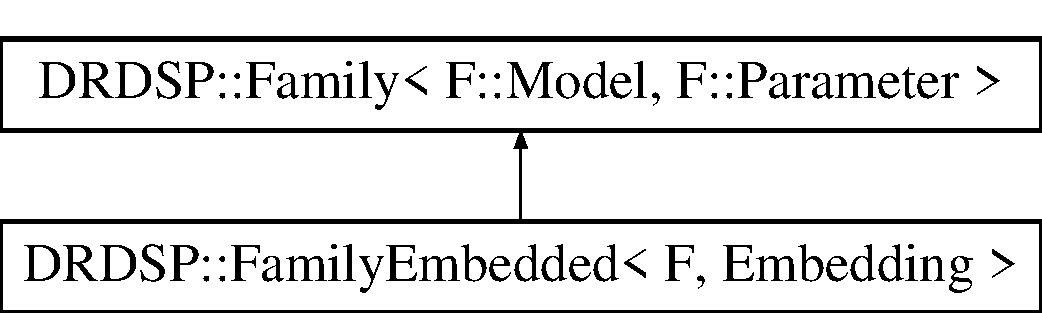
\includegraphics[height=2.000000cm]{struct_d_r_d_s_p_1_1_family_embedded}
\end{center}
\end{figure}
\subsection*{Public Member Functions}
\begin{DoxyCompactItemize}
\item 
\hypertarget{struct_d_r_d_s_p_1_1_family_embedded_af982885699e0b1737bc1e75b97c912c3}{{\bfseries Family\-Embedded} (const F \&f, const \hyperlink{struct_d_r_d_s_p_1_1_embedding}{Embedding} \&e)}\label{struct_d_r_d_s_p_1_1_family_embedded_af982885699e0b1737bc1e75b97c912c3}

\item 
\hypertarget{struct_d_r_d_s_p_1_1_family_embedded_a24c6c235505da6b4f27132d13f2c421a}{\hyperlink{struct_d_r_d_s_p_1_1_model_embedded}{Model\-Embedded}$<$ Model, \hyperlink{struct_d_r_d_s_p_1_1_embedding}{Embedding} $>$ {\bfseries operator()} (const Parameter \&parameter) const }\label{struct_d_r_d_s_p_1_1_family_embedded_a24c6c235505da6b4f27132d13f2c421a}

\end{DoxyCompactItemize}
\subsection*{Public Attributes}
\begin{DoxyCompactItemize}
\item 
\hypertarget{struct_d_r_d_s_p_1_1_family_embedded_af864495b07bc6181f422c290e322d055}{F \hyperlink{struct_d_r_d_s_p_1_1_family_embedded_af864495b07bc6181f422c290e322d055}{family}}\label{struct_d_r_d_s_p_1_1_family_embedded_af864495b07bc6181f422c290e322d055}

\begin{DoxyCompactList}\small\item\em The underlying family. \end{DoxyCompactList}\item 
\hypertarget{struct_d_r_d_s_p_1_1_family_embedded_a475108793c9f20f746263aed814c3651}{\hyperlink{struct_d_r_d_s_p_1_1_embedding}{Embedding} \hyperlink{struct_d_r_d_s_p_1_1_family_embedded_a475108793c9f20f746263aed814c3651}{embedding}}\label{struct_d_r_d_s_p_1_1_family_embedded_a475108793c9f20f746263aed814c3651}

\begin{DoxyCompactList}\small\item\em An embedding into R$^\wedge$n. \end{DoxyCompactList}\end{DoxyCompactItemize}
\subsection*{Additional Inherited Members}


\subsection{Detailed Description}
\subsubsection*{template$<$typename F, typename Embedding$>$struct D\-R\-D\-S\-P\-::\-Family\-Embedded$<$ F, Embedding $>$}

A model with parameters whose state space is embedded into R$^\wedge$n. 

The documentation for this struct was generated from the following file\-:\begin{DoxyCompactItemize}
\item 
include/\-D\-R\-D\-S\-P/dynamics/model.\-h\end{DoxyCompactItemize}

\hypertarget{struct_d_r_d_s_p_1_1_frobenius_inner_product}{\section{D\-R\-D\-S\-P\-:\-:Frobenius\-Inner\-Product Struct Reference}
\label{struct_d_r_d_s_p_1_1_frobenius_inner_product}\index{D\-R\-D\-S\-P\-::\-Frobenius\-Inner\-Product@{D\-R\-D\-S\-P\-::\-Frobenius\-Inner\-Product}}
}
\subsection*{Public Types}
\begin{DoxyCompactItemize}
\item 
\hypertarget{struct_d_r_d_s_p_1_1_frobenius_inner_product_aa8f7534db31acdcb6b8210af9cfa792c}{typedef Matrix\-Xd {\bfseries Vector}}\label{struct_d_r_d_s_p_1_1_frobenius_inner_product_aa8f7534db31acdcb6b8210af9cfa792c}

\item 
\hypertarget{struct_d_r_d_s_p_1_1_frobenius_inner_product_ac9b9c4144d29ddc883b4a8974c9189a7}{typedef Matrix\-Xd\-::\-Scalar {\bfseries Scalar}}\label{struct_d_r_d_s_p_1_1_frobenius_inner_product_ac9b9c4144d29ddc883b4a8974c9189a7}

\end{DoxyCompactItemize}
\subsection*{Public Member Functions}
\begin{DoxyCompactItemize}
\item 
\hypertarget{struct_d_r_d_s_p_1_1_frobenius_inner_product_adeedc7395fa902d0765c89bc98fe9e2a}{Scalar {\bfseries operator()} (const Matrix\-Xd \&x, const Matrix\-Xd \&y) const }\label{struct_d_r_d_s_p_1_1_frobenius_inner_product_adeedc7395fa902d0765c89bc98fe9e2a}

\item 
\hypertarget{struct_d_r_d_s_p_1_1_frobenius_inner_product_a506def98e9a9a220e78ee2bef3e8e68c}{Scalar {\bfseries Norm2} (const Matrix\-Xd \&x) const }\label{struct_d_r_d_s_p_1_1_frobenius_inner_product_a506def98e9a9a220e78ee2bef3e8e68c}

\end{DoxyCompactItemize}


The documentation for this struct was generated from the following file\-:\begin{DoxyCompactItemize}
\item 
include/\-D\-R\-D\-S\-P/geometry/metric.\-h\end{DoxyCompactItemize}

\hypertarget{struct_d_r_d_s_p_1_1_gaussian}{\section{D\-R\-D\-S\-P\-:\-:Gaussian Struct Reference}
\label{struct_d_r_d_s_p_1_1_gaussian}\index{D\-R\-D\-S\-P\-::\-Gaussian@{D\-R\-D\-S\-P\-::\-Gaussian}}
}
Inheritance diagram for D\-R\-D\-S\-P\-:\-:Gaussian\-:\begin{figure}[H]
\begin{center}
\leavevmode
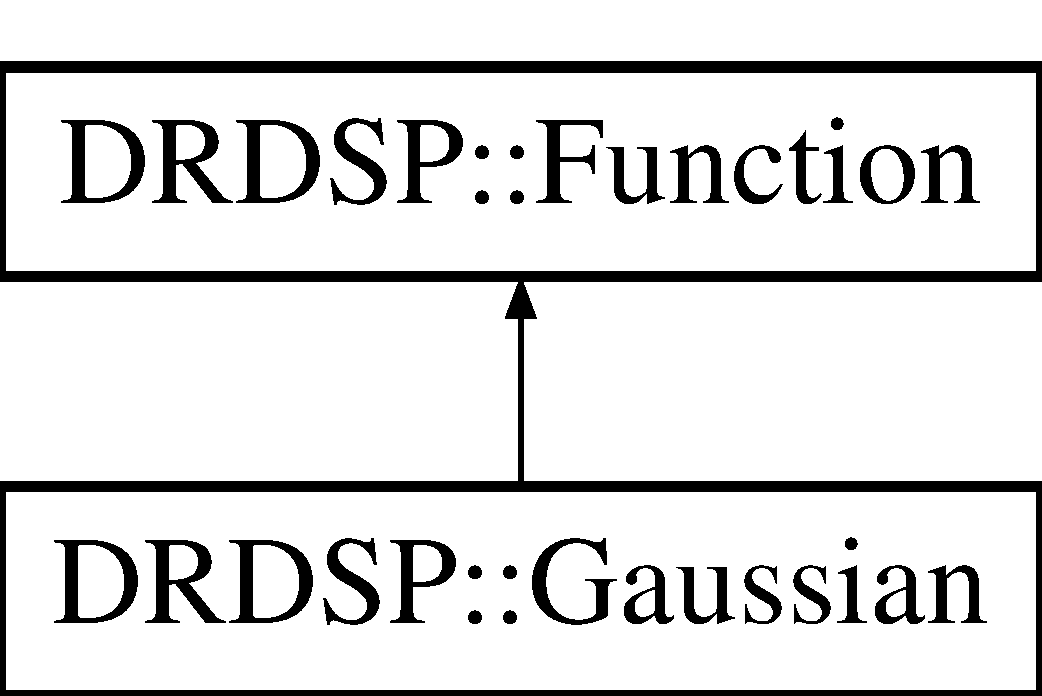
\includegraphics[height=2.000000cm]{struct_d_r_d_s_p_1_1_gaussian}
\end{center}
\end{figure}
\subsection*{Public Member Functions}
\begin{DoxyCompactItemize}
\item 
\hypertarget{struct_d_r_d_s_p_1_1_gaussian_aff703aa9e683cce46f56a41d173d2643}{double {\bfseries operator()} (double r) const }\label{struct_d_r_d_s_p_1_1_gaussian_aff703aa9e683cce46f56a41d173d2643}

\item 
\hypertarget{struct_d_r_d_s_p_1_1_gaussian_a9ae975cdc5b2bbc1ae2e1c3725f48890}{double {\bfseries Derivative} (double r) const }\label{struct_d_r_d_s_p_1_1_gaussian_a9ae975cdc5b2bbc1ae2e1c3725f48890}

\end{DoxyCompactItemize}
\subsection*{Public Attributes}
\begin{DoxyCompactItemize}
\item 
\hypertarget{struct_d_r_d_s_p_1_1_gaussian_a54c0ec40d9295e0167e6216912f01d2a}{double {\bfseries scale}}\label{struct_d_r_d_s_p_1_1_gaussian_a54c0ec40d9295e0167e6216912f01d2a}

\end{DoxyCompactItemize}


The documentation for this struct was generated from the following files\-:\begin{DoxyCompactItemize}
\item 
include/\-D\-R\-D\-S\-P/dynamics/radial\-\_\-basis.\-h\item 
src/dynamics/radial\-\_\-basis.\-cpp\end{DoxyCompactItemize}

\hypertarget{struct_d_r_d_s_p_1_1_grassmannian_1_1_geodesic}{\section{D\-R\-D\-S\-P\-:\-:Grassmannian\-:\-:Geodesic Struct Reference}
\label{struct_d_r_d_s_p_1_1_grassmannian_1_1_geodesic}\index{D\-R\-D\-S\-P\-::\-Grassmannian\-::\-Geodesic@{D\-R\-D\-S\-P\-::\-Grassmannian\-::\-Geodesic}}
}
\subsection*{Public Types}
\begin{DoxyCompactItemize}
\item 
\hypertarget{struct_d_r_d_s_p_1_1_grassmannian_1_1_geodesic_a4a0b6eae3786b1332a7d952124be1149}{typedef Metric {\bfseries Metric}}\label{struct_d_r_d_s_p_1_1_grassmannian_1_1_geodesic_a4a0b6eae3786b1332a7d952124be1149}

\item 
\hypertarget{struct_d_r_d_s_p_1_1_grassmannian_1_1_geodesic_a12af6f271811ddd9a4cf823d289adc87}{typedef double {\bfseries T}}\label{struct_d_r_d_s_p_1_1_grassmannian_1_1_geodesic_a12af6f271811ddd9a4cf823d289adc87}

\end{DoxyCompactItemize}
\subsection*{Public Member Functions}
\begin{DoxyCompactItemize}
\item 
\hypertarget{struct_d_r_d_s_p_1_1_grassmannian_1_1_geodesic_a035d24bba97ef7529ac731eb28ad3a0f}{{\bfseries Geodesic} (const Matrix\-Xd \&x, const Matrix\-Xd \&v)}\label{struct_d_r_d_s_p_1_1_grassmannian_1_1_geodesic_a035d24bba97ef7529ac731eb28ad3a0f}

\item 
\hypertarget{struct_d_r_d_s_p_1_1_grassmannian_1_1_geodesic_ab0ea4c98f06efd4350b46cea5ab473e9}{void {\bfseries Set} (const Matrix\-Xd \&x, const Matrix\-Xd \&v)}\label{struct_d_r_d_s_p_1_1_grassmannian_1_1_geodesic_ab0ea4c98f06efd4350b46cea5ab473e9}

\item 
\hypertarget{struct_d_r_d_s_p_1_1_grassmannian_1_1_geodesic_add97940011312bc74f12537afcfb81ea}{Matrix\-Xd {\bfseries operator()} (double t) const }\label{struct_d_r_d_s_p_1_1_grassmannian_1_1_geodesic_add97940011312bc74f12537afcfb81ea}

\item 
\hypertarget{struct_d_r_d_s_p_1_1_grassmannian_1_1_geodesic_afefc339d1c141b89794e59fa0c4237a9}{Matrix\-Xd {\bfseries Parallel\-Translate} (const Matrix\-Xd \&V, double t) const }\label{struct_d_r_d_s_p_1_1_grassmannian_1_1_geodesic_afefc339d1c141b89794e59fa0c4237a9}

\end{DoxyCompactItemize}
\subsection*{Public Attributes}
\begin{DoxyCompactItemize}
\item 
\hypertarget{struct_d_r_d_s_p_1_1_grassmannian_1_1_geodesic_abee018a46f9c7afb66d8b34738222dc1}{Matrix\-Xd {\bfseries position}}\label{struct_d_r_d_s_p_1_1_grassmannian_1_1_geodesic_abee018a46f9c7afb66d8b34738222dc1}

\item 
\hypertarget{struct_d_r_d_s_p_1_1_grassmannian_1_1_geodesic_acc96319d2d4ff34280463d23b56e4615}{Matrix\-Xd {\bfseries velocity}}\label{struct_d_r_d_s_p_1_1_grassmannian_1_1_geodesic_acc96319d2d4ff34280463d23b56e4615}

\end{DoxyCompactItemize}
\subsection*{Protected Types}
\begin{DoxyCompactItemize}
\item 
\hypertarget{struct_d_r_d_s_p_1_1_grassmannian_1_1_geodesic_a7ec327eb6529ec4ac20f7e5983aea099}{typedef Jacobi\-S\-V\-D$<$ Matrix\-Xd $>$\\*
\-::Singular\-Values\-Type {\bfseries sv\-Type}}\label{struct_d_r_d_s_p_1_1_grassmannian_1_1_geodesic_a7ec327eb6529ec4ac20f7e5983aea099}

\end{DoxyCompactItemize}
\subsection*{Protected Attributes}
\begin{DoxyCompactItemize}
\item 
\hypertarget{struct_d_r_d_s_p_1_1_grassmannian_1_1_geodesic_a830c4664220a4ac0e4b081c29d352215}{Jacobi\-S\-V\-D$<$ Matrix\-Xd $>$ {\bfseries svd}}\label{struct_d_r_d_s_p_1_1_grassmannian_1_1_geodesic_a830c4664220a4ac0e4b081c29d352215}

\end{DoxyCompactItemize}


The documentation for this struct was generated from the following files\-:\begin{DoxyCompactItemize}
\item 
include/\-D\-R\-D\-S\-P/geometry/grassmannian.\-h\item 
src/geometry/grassmannian.\-cpp\end{DoxyCompactItemize}

\hypertarget{struct_d_r_d_s_p_1_1_gradient_descent}{\section{D\-R\-D\-S\-P\-:\-:Gradient\-Descent$<$ T\-Geo, T\-Met $>$ Struct Template Reference}
\label{struct_d_r_d_s_p_1_1_gradient_descent}\index{D\-R\-D\-S\-P\-::\-Gradient\-Descent$<$ T\-Geo, T\-Met $>$@{D\-R\-D\-S\-P\-::\-Gradient\-Descent$<$ T\-Geo, T\-Met $>$}}
}
Inheritance diagram for D\-R\-D\-S\-P\-:\-:Gradient\-Descent$<$ T\-Geo, T\-Met $>$\-:\begin{figure}[H]
\begin{center}
\leavevmode
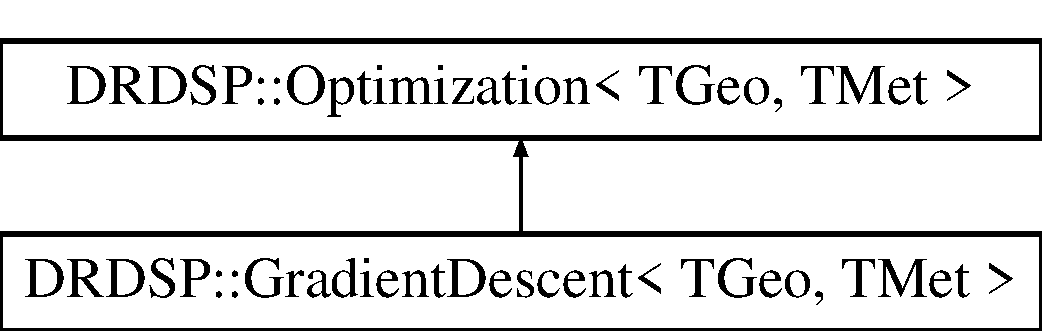
\includegraphics[height=2.000000cm]{struct_d_r_d_s_p_1_1_gradient_descent}
\end{center}
\end{figure}
\subsection*{Public Member Functions}
\begin{DoxyCompactItemize}
\item 
\hypertarget{struct_d_r_d_s_p_1_1_gradient_descent_a3e383660a94762cbee8bf8713c419dda}{bool {\bfseries Step} (T\-Vec \&X)}\label{struct_d_r_d_s_p_1_1_gradient_descent_a3e383660a94762cbee8bf8713c419dda}

\end{DoxyCompactItemize}
\subsection*{Additional Inherited Members}


The documentation for this struct was generated from the following file\-:\begin{DoxyCompactItemize}
\item 
include/\-D\-R\-D\-S\-P/optimization/gradient\-\_\-descent.\-h\end{DoxyCompactItemize}

\hypertarget{struct_d_r_d_s_p_1_1_histogram}{\section{D\-R\-D\-S\-P\-:\-:Histogram Struct Reference}
\label{struct_d_r_d_s_p_1_1_histogram}\index{D\-R\-D\-S\-P\-::\-Histogram@{D\-R\-D\-S\-P\-::\-Histogram}}
}


A histogram.  




{\ttfamily \#include $<$histogram.\-h$>$}

\subsection*{Public Member Functions}
\begin{DoxyCompactItemize}
\item 
\hypertarget{struct_d_r_d_s_p_1_1_histogram_aa66e25090948ef3e66fa909cd6c7137e}{{\bfseries Histogram} (uint32\-\_\-t n\-Bins)}\label{struct_d_r_d_s_p_1_1_histogram_aa66e25090948ef3e66fa909cd6c7137e}

\item 
\hypertarget{struct_d_r_d_s_p_1_1_histogram_abf0cc7d7101cead5c2fcacfa5ab6e432}{{\bfseries Histogram} (const \hyperlink{struct_d_r_d_s_p_1_1_histogram}{Histogram} \&rhs)}\label{struct_d_r_d_s_p_1_1_histogram_abf0cc7d7101cead5c2fcacfa5ab6e432}

\item 
\hypertarget{struct_d_r_d_s_p_1_1_histogram_a16a59db9ef1ba1e02d57afb81ed2d05c}{{\bfseries Histogram} (\hyperlink{struct_d_r_d_s_p_1_1_histogram}{Histogram} \&\&rhs)}\label{struct_d_r_d_s_p_1_1_histogram_a16a59db9ef1ba1e02d57afb81ed2d05c}

\item 
\hypertarget{struct_d_r_d_s_p_1_1_histogram_a32e47b8a29cd3e658a1b44e1c6253460}{\hyperlink{struct_d_r_d_s_p_1_1_histogram}{Histogram} \& {\bfseries operator=} (const \hyperlink{struct_d_r_d_s_p_1_1_histogram}{Histogram} \&rhs)}\label{struct_d_r_d_s_p_1_1_histogram_a32e47b8a29cd3e658a1b44e1c6253460}

\item 
\hypertarget{struct_d_r_d_s_p_1_1_histogram_a3f705b4ad8eafb893a760abf7a55dcfe}{\hyperlink{struct_d_r_d_s_p_1_1_histogram}{Histogram} \& {\bfseries operator=} (\hyperlink{struct_d_r_d_s_p_1_1_histogram}{Histogram} \&\&rhs)}\label{struct_d_r_d_s_p_1_1_histogram_a3f705b4ad8eafb893a760abf7a55dcfe}

\item 
\hypertarget{struct_d_r_d_s_p_1_1_histogram_a11252e6e91d54a93766eab33756e46fd}{void {\bfseries Create} (uint32\-\_\-t n\-Bins)}\label{struct_d_r_d_s_p_1_1_histogram_a11252e6e91d54a93766eab33756e46fd}

\item 
\hypertarget{struct_d_r_d_s_p_1_1_histogram_a84577ee394d1017b16aa4229ff7f5904}{void {\bfseries Destroy} ()}\label{struct_d_r_d_s_p_1_1_histogram_a84577ee394d1017b16aa4229ff7f5904}

\item 
\hypertarget{struct_d_r_d_s_p_1_1_histogram_adeb7a588aa66fe2e6dd0d851ea92d625}{uint32\-\_\-t {\bfseries Total\-Frequency} () const }\label{struct_d_r_d_s_p_1_1_histogram_adeb7a588aa66fe2e6dd0d851ea92d625}

\item 
\hypertarget{struct_d_r_d_s_p_1_1_histogram_a849de9ad07ff6c468dad15a9951a3f81}{void \hyperlink{struct_d_r_d_s_p_1_1_histogram_a849de9ad07ff6c468dad15a9951a3f81}{Write\-C\-S\-V} (const char $\ast$filename) const }\label{struct_d_r_d_s_p_1_1_histogram_a849de9ad07ff6c468dad15a9951a3f81}

\begin{DoxyCompactList}\small\item\em Sums the bin frequencies. \end{DoxyCompactList}\end{DoxyCompactItemize}
\subsection*{Public Attributes}
\begin{DoxyCompactItemize}
\item 
\hypertarget{struct_d_r_d_s_p_1_1_histogram_a22b2c10bc25d799a1d32dec46887dcb0}{\hyperlink{struct_d_r_d_s_p_1_1_bin}{Bin} $\ast$ {\bfseries bins}}\label{struct_d_r_d_s_p_1_1_histogram_a22b2c10bc25d799a1d32dec46887dcb0}

\item 
\hypertarget{struct_d_r_d_s_p_1_1_histogram_a0958a362ffa72e63c899f6622c2aa638}{uint32\-\_\-t {\bfseries num\-Bins}}\label{struct_d_r_d_s_p_1_1_histogram_a0958a362ffa72e63c899f6622c2aa638}

\end{DoxyCompactItemize}


\subsection{Detailed Description}
A histogram. 

This is just an array of bins with some helper functions. 

The documentation for this struct was generated from the following files\-:\begin{DoxyCompactItemize}
\item 
include/\-D\-R\-D\-S\-P/data/histogram.\-h\item 
src/data/histogram.\-cpp\end{DoxyCompactItemize}

\hypertarget{struct_d_r_d_s_p_1_1_histogram_generator}{\section{D\-R\-D\-S\-P\-:\-:Histogram\-Generator Struct Reference}
\label{struct_d_r_d_s_p_1_1_histogram_generator}\index{D\-R\-D\-S\-P\-::\-Histogram\-Generator@{D\-R\-D\-S\-P\-::\-Histogram\-Generator}}
}


A class for generating histograms from data.  




{\ttfamily \#include $<$histogram.\-h$>$}

\subsection*{Public Member Functions}
\begin{DoxyCompactItemize}
\item 
\hypertarget{struct_d_r_d_s_p_1_1_histogram_generator_a9eda2d2c8db47d55b32eee8033f5f268}{{\bfseries Histogram\-Generator} (uint32\-\_\-t n\-Bins)}\label{struct_d_r_d_s_p_1_1_histogram_generator_a9eda2d2c8db47d55b32eee8033f5f268}

\item 
\hypertarget{struct_d_r_d_s_p_1_1_histogram_generator_af1acac305990b01bc4cc6e612415bf72}{\hyperlink{struct_d_r_d_s_p_1_1_histogram}{Histogram} \hyperlink{struct_d_r_d_s_p_1_1_histogram_generator_af1acac305990b01bc4cc6e612415bf72}{Generate} (const double $\ast$data, size\-\_\-t N) const }\label{struct_d_r_d_s_p_1_1_histogram_generator_af1acac305990b01bc4cc6e612415bf72}

\begin{DoxyCompactList}\small\item\em Generates a histogram from the given data. \end{DoxyCompactList}\item 
\hypertarget{struct_d_r_d_s_p_1_1_histogram_generator_a145bb9b1ea633982ef24849107988c09}{\hyperlink{struct_d_r_d_s_p_1_1_histogram}{Histogram} \hyperlink{struct_d_r_d_s_p_1_1_histogram_generator_a145bb9b1ea633982ef24849107988c09}{Generate} (const vector$<$ double $>$ \&data) const }\label{struct_d_r_d_s_p_1_1_histogram_generator_a145bb9b1ea633982ef24849107988c09}

\begin{DoxyCompactList}\small\item\em Generates a histogram from the given data. \end{DoxyCompactList}\end{DoxyCompactItemize}
\subsection*{Public Attributes}
\begin{DoxyCompactItemize}
\item 
\hypertarget{struct_d_r_d_s_p_1_1_histogram_generator_a2f6b01668e743ce436f54c3ca56275a1}{uint32\-\_\-t \hyperlink{struct_d_r_d_s_p_1_1_histogram_generator_a2f6b01668e743ce436f54c3ca56275a1}{num\-Bins} = 0}\label{struct_d_r_d_s_p_1_1_histogram_generator_a2f6b01668e743ce436f54c3ca56275a1}

\begin{DoxyCompactList}\small\item\em The number of bins that we want the histogram to contain. \end{DoxyCompactList}\item 
\hypertarget{struct_d_r_d_s_p_1_1_histogram_generator_aef85198c4644dbcfa27d24e9015bb025}{double {\bfseries clamp\-Min} = 0}\label{struct_d_r_d_s_p_1_1_histogram_generator_aef85198c4644dbcfa27d24e9015bb025}

\item 
\hypertarget{struct_d_r_d_s_p_1_1_histogram_generator_a5cec8e7e75d95a66b4a17c3f70c2b556}{double \hyperlink{struct_d_r_d_s_p_1_1_histogram_generator_a5cec8e7e75d95a66b4a17c3f70c2b556}{clamp\-Max} = 0}\label{struct_d_r_d_s_p_1_1_histogram_generator_a5cec8e7e75d95a66b4a17c3f70c2b556}

\begin{DoxyCompactList}\small\item\em clamping limits the range of the bins \end{DoxyCompactList}\item 
\hypertarget{struct_d_r_d_s_p_1_1_histogram_generator_a12fe0ce6860a6f8bd17b1355f91c0ac6}{bool \hyperlink{struct_d_r_d_s_p_1_1_histogram_generator_a12fe0ce6860a6f8bd17b1355f91c0ac6}{clamp} = false}\label{struct_d_r_d_s_p_1_1_histogram_generator_a12fe0ce6860a6f8bd17b1355f91c0ac6}

\begin{DoxyCompactList}\small\item\em Perform clamping. \end{DoxyCompactList}\item 
\hypertarget{struct_d_r_d_s_p_1_1_histogram_generator_a84935b50902a985afdeca6541bac8c06}{bool \hyperlink{struct_d_r_d_s_p_1_1_histogram_generator_a84935b50902a985afdeca6541bac8c06}{log\-Scale} = false}\label{struct_d_r_d_s_p_1_1_histogram_generator_a84935b50902a985afdeca6541bac8c06}

\begin{DoxyCompactList}\small\item\em Use a logarithmic scale for the bin sizes. \end{DoxyCompactList}\end{DoxyCompactItemize}


\subsection{Detailed Description}
A class for generating histograms from data. 

The documentation for this struct was generated from the following files\-:\begin{DoxyCompactItemize}
\item 
include/\-D\-R\-D\-S\-P/data/histogram.\-h\item 
src/data/histogram.\-cpp\end{DoxyCompactItemize}

\hypertarget{struct_d_r_d_s_p_1_1_identity_embedding}{\section{D\-R\-D\-S\-P\-:\-:Identity\-Embedding Struct Reference}
\label{struct_d_r_d_s_p_1_1_identity_embedding}\index{D\-R\-D\-S\-P\-::\-Identity\-Embedding@{D\-R\-D\-S\-P\-::\-Identity\-Embedding}}
}
Inheritance diagram for D\-R\-D\-S\-P\-:\-:Identity\-Embedding\-:\begin{figure}[H]
\begin{center}
\leavevmode
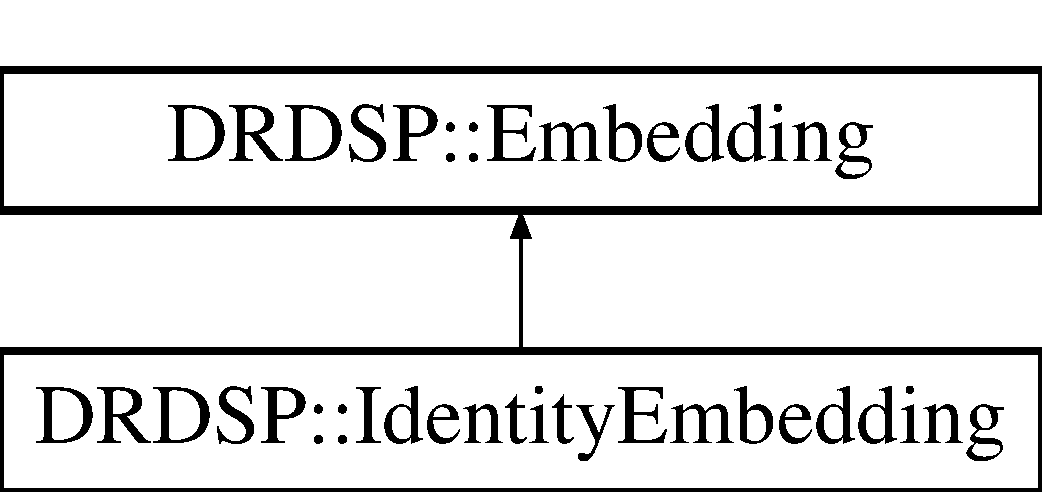
\includegraphics[height=2.000000cm]{struct_d_r_d_s_p_1_1_identity_embedding}
\end{center}
\end{figure}
\subsection*{Public Member Functions}
\begin{DoxyCompactItemize}
\item 
\hypertarget{struct_d_r_d_s_p_1_1_identity_embedding_ab0e013dd16519f519ba32f38f1e743a3}{{\bfseries Identity\-Embedding} (uint32\-\_\-t dim)}\label{struct_d_r_d_s_p_1_1_identity_embedding_ab0e013dd16519f519ba32f38f1e743a3}

\item 
\hypertarget{struct_d_r_d_s_p_1_1_identity_embedding_aaed08501ed449445888d8e8776c69f4f}{Vector\-Xd {\bfseries operator()} (const Vector\-Xd \&x) const }\label{struct_d_r_d_s_p_1_1_identity_embedding_aaed08501ed449445888d8e8776c69f4f}

\item 
\hypertarget{struct_d_r_d_s_p_1_1_identity_embedding_a41bad0cd08f274f78412a31e0fb6854e}{Matrix\-Xd {\bfseries Derivative} (const Vector\-Xd \&) const }\label{struct_d_r_d_s_p_1_1_identity_embedding_a41bad0cd08f274f78412a31e0fb6854e}

\item 
\hypertarget{struct_d_r_d_s_p_1_1_identity_embedding_a836b4855538770d5f2d40e2c294c5b88}{Matrix\-Xd {\bfseries Derivative\-Adjoint} (const Vector\-Xd \&) const }\label{struct_d_r_d_s_p_1_1_identity_embedding_a836b4855538770d5f2d40e2c294c5b88}

\item 
\hypertarget{struct_d_r_d_s_p_1_1_identity_embedding_a62a97e69aa9aa28c5d4f3dc60cb5359e}{Matrix\-Xd {\bfseries Derivative2} (const Vector\-Xd \&, uint32\-\_\-t) const }\label{struct_d_r_d_s_p_1_1_identity_embedding_a62a97e69aa9aa28c5d4f3dc60cb5359e}

\end{DoxyCompactItemize}
\subsection*{Additional Inherited Members}


The documentation for this struct was generated from the following file\-:\begin{DoxyCompactItemize}
\item 
include/\-D\-R\-D\-S\-P/dynamics/embedding.\-h\end{DoxyCompactItemize}

\hypertarget{struct_d_r_d_s_p_1_1_identity_wrap_function}{\section{D\-R\-D\-S\-P\-:\-:Identity\-Wrap\-Function Struct Reference}
\label{struct_d_r_d_s_p_1_1_identity_wrap_function}\index{D\-R\-D\-S\-P\-::\-Identity\-Wrap\-Function@{D\-R\-D\-S\-P\-::\-Identity\-Wrap\-Function}}
}
\subsection*{Public Member Functions}
\begin{DoxyCompactItemize}
\item 
\hypertarget{struct_d_r_d_s_p_1_1_identity_wrap_function_a3ad8e117a048d95b1c5911a4a1f1305b}{{\footnotesize template$<$typename T $>$ }\\void {\bfseries operator()} (T \&) const }\label{struct_d_r_d_s_p_1_1_identity_wrap_function_a3ad8e117a048d95b1c5911a4a1f1305b}

\end{DoxyCompactItemize}


The documentation for this struct was generated from the following file\-:\begin{DoxyCompactItemize}
\item 
include/\-D\-R\-D\-S\-P/dynamics/dynamical\-System.\-h\end{DoxyCompactItemize}

\hypertarget{struct_d_r_d_s_p_1_1_inverse_multiquadratic}{\section{D\-R\-D\-S\-P\-:\-:Inverse\-Multiquadratic Struct Reference}
\label{struct_d_r_d_s_p_1_1_inverse_multiquadratic}\index{D\-R\-D\-S\-P\-::\-Inverse\-Multiquadratic@{D\-R\-D\-S\-P\-::\-Inverse\-Multiquadratic}}
}
\subsection*{Public Member Functions}
\begin{DoxyCompactItemize}
\item 
\hypertarget{struct_d_r_d_s_p_1_1_inverse_multiquadratic_a9de4a748cfda8c1bd8c0dfca408faed7}{{\bfseries Inverse\-Multiquadratic} (double scale)}\label{struct_d_r_d_s_p_1_1_inverse_multiquadratic_a9de4a748cfda8c1bd8c0dfca408faed7}

\item 
\hypertarget{struct_d_r_d_s_p_1_1_inverse_multiquadratic_a5ced1f6abf959202569facafb56be592}{{\footnotesize template$<$typename T $>$ }\\T {\bfseries operator()} (T r) const }\label{struct_d_r_d_s_p_1_1_inverse_multiquadratic_a5ced1f6abf959202569facafb56be592}

\item 
\hypertarget{struct_d_r_d_s_p_1_1_inverse_multiquadratic_abf5407eb574dbac34ad1cbd07f59be50}{{\footnotesize template$<$typename T $>$ }\\T {\bfseries Derivative} (T r) const }\label{struct_d_r_d_s_p_1_1_inverse_multiquadratic_abf5407eb574dbac34ad1cbd07f59be50}

\end{DoxyCompactItemize}
\subsection*{Public Attributes}
\begin{DoxyCompactItemize}
\item 
\hypertarget{struct_d_r_d_s_p_1_1_inverse_multiquadratic_a39009875f833958785889ac9373ad37c}{double {\bfseries scale}}\label{struct_d_r_d_s_p_1_1_inverse_multiquadratic_a39009875f833958785889ac9373ad37c}

\end{DoxyCompactItemize}


The documentation for this struct was generated from the following file\-:\begin{DoxyCompactItemize}
\item 
include/\-D\-R\-D\-S\-P/dynamics/radial\-\_\-basis.\-h\end{DoxyCompactItemize}

\hypertarget{struct_d_r_d_s_p_1_1_inverse_quadratic}{\section{D\-R\-D\-S\-P\-:\-:Inverse\-Quadratic Struct Reference}
\label{struct_d_r_d_s_p_1_1_inverse_quadratic}\index{D\-R\-D\-S\-P\-::\-Inverse\-Quadratic@{D\-R\-D\-S\-P\-::\-Inverse\-Quadratic}}
}
\subsection*{Public Member Functions}
\begin{DoxyCompactItemize}
\item 
\hypertarget{struct_d_r_d_s_p_1_1_inverse_quadratic_a8046e278ab0c485750ff062c6862ec87}{double {\bfseries operator()} (double r) const }\label{struct_d_r_d_s_p_1_1_inverse_quadratic_a8046e278ab0c485750ff062c6862ec87}

\item 
\hypertarget{struct_d_r_d_s_p_1_1_inverse_quadratic_a628c78a421c55898e94846eeb1865326}{double {\bfseries Derivative} (double r) const }\label{struct_d_r_d_s_p_1_1_inverse_quadratic_a628c78a421c55898e94846eeb1865326}

\end{DoxyCompactItemize}
\subsection*{Public Attributes}
\begin{DoxyCompactItemize}
\item 
\hypertarget{struct_d_r_d_s_p_1_1_inverse_quadratic_a31241ecd1ec571b651307d29e6b69c07}{double {\bfseries scale}}\label{struct_d_r_d_s_p_1_1_inverse_quadratic_a31241ecd1ec571b651307d29e6b69c07}

\end{DoxyCompactItemize}


The documentation for this struct was generated from the following files\-:\begin{DoxyCompactItemize}
\item 
include/\-D\-R\-D\-S\-P/dynamics/radial\-\_\-basis.\-h\item 
src/dynamics/radial\-\_\-basis.\-cpp\end{DoxyCompactItemize}

\hypertarget{struct_d_r_d_s_p_1_1_line_search}{\section{D\-R\-D\-S\-P\-:\-:Line\-Search$<$ T\-Met $>$ Struct Template Reference}
\label{struct_d_r_d_s_p_1_1_line_search}\index{D\-R\-D\-S\-P\-::\-Line\-Search$<$ T\-Met $>$@{D\-R\-D\-S\-P\-::\-Line\-Search$<$ T\-Met $>$}}
}
\subsection*{Public Types}
\begin{DoxyCompactItemize}
\item 
\hypertarget{struct_d_r_d_s_p_1_1_line_search_a0a4f464ca776f11974fbe1bf8b5b10ef}{typedef T\-Met\-::\-T\-Vec {\bfseries T\-Vec}}\label{struct_d_r_d_s_p_1_1_line_search_a0a4f464ca776f11974fbe1bf8b5b10ef}

\end{DoxyCompactItemize}
\subsection*{Public Member Functions}
\begin{DoxyCompactItemize}
\item 
\hypertarget{struct_d_r_d_s_p_1_1_line_search_a11c98ca28033eb725eb0f8c0c2165415}{{\bfseries Line\-Search} (\hyperlink{struct_d_r_d_s_p_1_1_geodesic}{Geodesic}$<$ T\-Vec $>$ $\ast$geodesic)}\label{struct_d_r_d_s_p_1_1_line_search_a11c98ca28033eb725eb0f8c0c2165415}

\item 
\hypertarget{struct_d_r_d_s_p_1_1_line_search_a4ea0db15193335a91e76b2e6460eac14}{double {\bfseries Deriv\-S} (const T\-Vec \&X, const T\-Vec \&V)}\label{struct_d_r_d_s_p_1_1_line_search_a4ea0db15193335a91e76b2e6460eac14}

\item 
\hypertarget{struct_d_r_d_s_p_1_1_line_search_ab33f387294ebe3f8fe93a1a35b86bca3}{double {\bfseries Search} ()}\label{struct_d_r_d_s_p_1_1_line_search_ab33f387294ebe3f8fe93a1a35b86bca3}

\end{DoxyCompactItemize}
\subsection*{Public Attributes}
\begin{DoxyCompactItemize}
\item 
\hypertarget{struct_d_r_d_s_p_1_1_line_search_aeeb734f0f9cfb12bb1012900d86b6ad3}{double($\ast$ {\bfseries S} )(const T\-Vec \&X, const void $\ast$obj)}\label{struct_d_r_d_s_p_1_1_line_search_aeeb734f0f9cfb12bb1012900d86b6ad3}

\item 
\hypertarget{struct_d_r_d_s_p_1_1_line_search_aa58cdd4d0ac6bb29c91013bf3e036511}{T\-Vec($\ast$ {\bfseries grad\-S} )(const T\-Vec \&X, const void $\ast$obj)}\label{struct_d_r_d_s_p_1_1_line_search_aa58cdd4d0ac6bb29c91013bf3e036511}

\item 
\hypertarget{struct_d_r_d_s_p_1_1_line_search_a5b4fc5bf7eec402586369be822ac471d}{const void $\ast$ {\bfseries obj}}\label{struct_d_r_d_s_p_1_1_line_search_a5b4fc5bf7eec402586369be822ac471d}

\item 
\hypertarget{struct_d_r_d_s_p_1_1_line_search_a97269c9395582cd1e5686b2bb88357b7}{const T\-Met $\ast$ {\bfseries metric}}\label{struct_d_r_d_s_p_1_1_line_search_a97269c9395582cd1e5686b2bb88357b7}

\item 
\hypertarget{struct_d_r_d_s_p_1_1_line_search_a69072580c2272d7dc555b89a727e575d}{T\-Vec {\bfseries grad\-Sx}}\label{struct_d_r_d_s_p_1_1_line_search_a69072580c2272d7dc555b89a727e575d}

\item 
\hypertarget{struct_d_r_d_s_p_1_1_line_search_a86391914be1b243831bd5227cca39513}{double {\bfseries Sx}}\label{struct_d_r_d_s_p_1_1_line_search_a86391914be1b243831bd5227cca39513}

\item 
\hypertarget{struct_d_r_d_s_p_1_1_line_search_aae7c2b8bcd865b0a6aba7754ace51073}{double {\bfseries alpha}}\label{struct_d_r_d_s_p_1_1_line_search_aae7c2b8bcd865b0a6aba7754ace51073}

\end{DoxyCompactItemize}
\subsection*{Protected Member Functions}
\begin{DoxyCompactItemize}
\item 
\hypertarget{struct_d_r_d_s_p_1_1_line_search_a3ccc22ae4853a6b617ca2e13bda842f2}{bool {\bfseries Wolfe} (double Sc, double gc)}\label{struct_d_r_d_s_p_1_1_line_search_a3ccc22ae4853a6b617ca2e13bda842f2}

\item 
\hypertarget{struct_d_r_d_s_p_1_1_line_search_a3b1a2771360efeaf9434479b0df9fbf1}{double {\bfseries Secant} (double a, double b, double ga, double gb)}\label{struct_d_r_d_s_p_1_1_line_search_a3b1a2771360efeaf9434479b0df9fbf1}

\item 
\hypertarget{struct_d_r_d_s_p_1_1_line_search_a202ae4e26b280c839008a5021e7afa67}{double {\bfseries Riddler} (double x1, double x2, double x3, double gx1, double gx2, double gx3)}\label{struct_d_r_d_s_p_1_1_line_search_a202ae4e26b280c839008a5021e7afa67}

\end{DoxyCompactItemize}
\subsection*{Protected Attributes}
\begin{DoxyCompactItemize}
\item 
\hypertarget{struct_d_r_d_s_p_1_1_line_search_a0512b9941dfb6af38a9bf1296904d7eb}{\hyperlink{struct_d_r_d_s_p_1_1_geodesic}{Geodesic}$<$ T\-Vec $>$ $\ast$ {\bfseries G}}\label{struct_d_r_d_s_p_1_1_line_search_a0512b9941dfb6af38a9bf1296904d7eb}

\item 
\hypertarget{struct_d_r_d_s_p_1_1_line_search_a4872eda50336fe3573d2118d3b929ef0}{double {\bfseries deriv\-Sx}}\label{struct_d_r_d_s_p_1_1_line_search_a4872eda50336fe3573d2118d3b929ef0}

\item 
\hypertarget{struct_d_r_d_s_p_1_1_line_search_a7cb4acca18846268383c8e579bb58260}{double {\bfseries mu}}\label{struct_d_r_d_s_p_1_1_line_search_a7cb4acca18846268383c8e579bb58260}

\item 
\hypertarget{struct_d_r_d_s_p_1_1_line_search_a05c6aafb2cd71e6b9bac7dcc1724986e}{double {\bfseries eta}}\label{struct_d_r_d_s_p_1_1_line_search_a05c6aafb2cd71e6b9bac7dcc1724986e}

\item 
\hypertarget{struct_d_r_d_s_p_1_1_line_search_aa5f9dd44b7ef2c694469b31f3e7ee9d7}{double {\bfseries alpha\-Max}}\label{struct_d_r_d_s_p_1_1_line_search_aa5f9dd44b7ef2c694469b31f3e7ee9d7}

\end{DoxyCompactItemize}


The documentation for this struct was generated from the following file\-:\begin{DoxyCompactItemize}
\item 
include/\-D\-R\-D\-S\-P/optimization/linesearch.\-h\end{DoxyCompactItemize}

\hypertarget{struct_d_r_d_s_p_1_1_model}{\section{D\-R\-D\-S\-P\-:\-:Model$<$ State $>$ Struct Template Reference}
\label{struct_d_r_d_s_p_1_1_model}\index{D\-R\-D\-S\-P\-::\-Model$<$ State $>$@{D\-R\-D\-S\-P\-::\-Model$<$ State $>$}}
}


Base for model without parameters.  




{\ttfamily \#include $<$model.\-h$>$}

\subsection*{Public Types}
\begin{DoxyCompactItemize}
\item 
\hypertarget{struct_d_r_d_s_p_1_1_model_a30ca6d1a4dbcb6801ccb5a2421cbc434}{typedef State {\bfseries State}}\label{struct_d_r_d_s_p_1_1_model_a30ca6d1a4dbcb6801ccb5a2421cbc434}

\end{DoxyCompactItemize}
\subsection*{Public Member Functions}
\begin{DoxyCompactItemize}
\item 
\hypertarget{struct_d_r_d_s_p_1_1_model_aa14d5a47ab0d94ab7c17ffe9c50125a4}{{\bfseries Model} (uint32\-\_\-t \hyperlink{struct_d_r_d_s_p_1_1_model_a5689ac0bda80d0ae6db69443439ce1b5}{state\-Dim})}\label{struct_d_r_d_s_p_1_1_model_aa14d5a47ab0d94ab7c17ffe9c50125a4}

\end{DoxyCompactItemize}
\subsection*{Public Attributes}
\begin{DoxyCompactItemize}
\item 
\hypertarget{struct_d_r_d_s_p_1_1_model_a5689ac0bda80d0ae6db69443439ce1b5}{uint32\-\_\-t \hyperlink{struct_d_r_d_s_p_1_1_model_a5689ac0bda80d0ae6db69443439ce1b5}{state\-Dim}}\label{struct_d_r_d_s_p_1_1_model_a5689ac0bda80d0ae6db69443439ce1b5}

\begin{DoxyCompactList}\small\item\em Dimension of the model's state space. \end{DoxyCompactList}\end{DoxyCompactItemize}


\subsection{Detailed Description}
\subsubsection*{template$<$typename State = Vector\-Xd$>$struct D\-R\-D\-S\-P\-::\-Model$<$ State $>$}

Base for model without parameters. 

The documentation for this struct was generated from the following file\-:\begin{DoxyCompactItemize}
\item 
include/\-D\-R\-D\-S\-P/dynamics/model.\-h\end{DoxyCompactItemize}

\hypertarget{struct_d_r_d_s_p_1_1_model_embedded}{\section{D\-R\-D\-S\-P\-:\-:Model\-Embedded Struct Reference}
\label{struct_d_r_d_s_p_1_1_model_embedded}\index{D\-R\-D\-S\-P\-::\-Model\-Embedded@{D\-R\-D\-S\-P\-::\-Model\-Embedded}}
}


A model without parameters whose state space is embedded into R$^\wedge$n.  




{\ttfamily \#include $<$model.\-h$>$}

\subsection*{Public Member Functions}
\begin{DoxyCompactItemize}
\item 
\hypertarget{struct_d_r_d_s_p_1_1_model_embedded_aac8110fc1d52b006311cc1ca9377a8d4}{{\bfseries Model\-Embedded} (\hyperlink{struct_d_r_d_s_p_1_1_model}{Model} \&m, \hyperlink{struct_d_r_d_s_p_1_1_embedding}{Embedding} \&e)}\label{struct_d_r_d_s_p_1_1_model_embedded_aac8110fc1d52b006311cc1ca9377a8d4}

\item 
\hypertarget{struct_d_r_d_s_p_1_1_model_embedded_a4f33e3c6473e997ae92c75771aa918fd}{Vector\-Xd \hyperlink{struct_d_r_d_s_p_1_1_model_embedded_a4f33e3c6473e997ae92c75771aa918fd}{Vector\-Field} (const Vector\-Xd \&state)}\label{struct_d_r_d_s_p_1_1_model_embedded_a4f33e3c6473e997ae92c75771aa918fd}

\begin{DoxyCompactList}\small\item\em The vector field on R$^\wedge$n. \end{DoxyCompactList}\item 
\hypertarget{struct_d_r_d_s_p_1_1_model_embedded_a6aaa71ce7c8a2b11f86e7950498249c0}{Matrix\-Xd \hyperlink{struct_d_r_d_s_p_1_1_model_embedded_a6aaa71ce7c8a2b11f86e7950498249c0}{Partials} (const Vector\-Xd \&state)}\label{struct_d_r_d_s_p_1_1_model_embedded_a6aaa71ce7c8a2b11f86e7950498249c0}

\begin{DoxyCompactList}\small\item\em The partial derivative of the vector field on R$^\wedge$n with respect to the underlying state. \end{DoxyCompactList}\end{DoxyCompactItemize}
\subsection*{Public Attributes}
\begin{DoxyCompactItemize}
\item 
\hypertarget{struct_d_r_d_s_p_1_1_model_embedded_a2d021cf215cdd084fde36bbd46101cc5}{\hyperlink{struct_d_r_d_s_p_1_1_model}{Model} \& \hyperlink{struct_d_r_d_s_p_1_1_model_embedded_a2d021cf215cdd084fde36bbd46101cc5}{model}}\label{struct_d_r_d_s_p_1_1_model_embedded_a2d021cf215cdd084fde36bbd46101cc5}

\begin{DoxyCompactList}\small\item\em The underlying model. \end{DoxyCompactList}\item 
\hypertarget{struct_d_r_d_s_p_1_1_model_embedded_a22aeda6bb7f303b3e79a6f133887439b}{\hyperlink{struct_d_r_d_s_p_1_1_embedding}{Embedding} \& \hyperlink{struct_d_r_d_s_p_1_1_model_embedded_a22aeda6bb7f303b3e79a6f133887439b}{embedding}}\label{struct_d_r_d_s_p_1_1_model_embedded_a22aeda6bb7f303b3e79a6f133887439b}

\begin{DoxyCompactList}\small\item\em An embedding into R$^\wedge$n. \end{DoxyCompactList}\end{DoxyCompactItemize}


\subsection{Detailed Description}
A model without parameters whose state space is embedded into R$^\wedge$n. 

The documentation for this struct was generated from the following files\-:\begin{DoxyCompactItemize}
\item 
include/\-D\-R\-D\-S\-P/dynamics/model.\-h\item 
src/dynamics/model.\-cpp\end{DoxyCompactItemize}

\hypertarget{struct_d_r_d_s_p_1_1_multiquadratic}{\section{D\-R\-D\-S\-P\-:\-:Multiquadratic Struct Reference}
\label{struct_d_r_d_s_p_1_1_multiquadratic}\index{D\-R\-D\-S\-P\-::\-Multiquadratic@{D\-R\-D\-S\-P\-::\-Multiquadratic}}
}
\subsection*{Public Member Functions}
\begin{DoxyCompactItemize}
\item 
\hypertarget{struct_d_r_d_s_p_1_1_multiquadratic_a9676531016bae341f6c2e9163041b899}{{\bfseries Multiquadratic} (double scale)}\label{struct_d_r_d_s_p_1_1_multiquadratic_a9676531016bae341f6c2e9163041b899}

\item 
\hypertarget{struct_d_r_d_s_p_1_1_multiquadratic_af06319ae007aa40fbd2833759161437f}{double {\bfseries operator()} (double r) const }\label{struct_d_r_d_s_p_1_1_multiquadratic_af06319ae007aa40fbd2833759161437f}

\item 
\hypertarget{struct_d_r_d_s_p_1_1_multiquadratic_afba9d7a5aeb541953b9a54919b013f5f}{double {\bfseries Derivative} (double r) const }\label{struct_d_r_d_s_p_1_1_multiquadratic_afba9d7a5aeb541953b9a54919b013f5f}

\end{DoxyCompactItemize}
\subsection*{Public Attributes}
\begin{DoxyCompactItemize}
\item 
\hypertarget{struct_d_r_d_s_p_1_1_multiquadratic_ad075ed2b3b85cab9d74369163eab65cf}{double {\bfseries scale}}\label{struct_d_r_d_s_p_1_1_multiquadratic_ad075ed2b3b85cab9d74369163eab65cf}

\end{DoxyCompactItemize}


The documentation for this struct was generated from the following files\-:\begin{DoxyCompactItemize}
\item 
include/\-D\-R\-D\-S\-P/dynamics/radial\-\_\-basis.\-h\item 
src/dynamics/radial\-\_\-basis.\-cpp\end{DoxyCompactItemize}

\hypertarget{struct_eigen_1_1_num_traits_3_01dual_3_01_t_01_4_01_4}{\section{Eigen\-:\-:Num\-Traits$<$ dual$<$ T $>$ $>$ Struct Template Reference}
\label{struct_eigen_1_1_num_traits_3_01dual_3_01_t_01_4_01_4}\index{Eigen\-::\-Num\-Traits$<$ dual$<$ T $>$ $>$@{Eigen\-::\-Num\-Traits$<$ dual$<$ T $>$ $>$}}
}
\subsection*{Public Types}
\begin{DoxyCompactItemize}
\item 
enum \{ \\*
{\bfseries Is\-Integer} = 0, 
{\bfseries Is\-Signed} = 1, 
{\bfseries Is\-Complex} = 0, 
{\bfseries Require\-Initialization} = Num\-Traits$<$T$>$\-:\-:Require\-Initialization, 
\\*
{\bfseries Read\-Cost} = 2 $\ast$ Num\-Traits$<$T$>$\-:\-:Read\-Cost, 
{\bfseries Add\-Cost} = 2 $\ast$ Num\-Traits$<$T$>$\-:\-:Add\-Cost, 
{\bfseries Mul\-Cost} = 3 $\ast$ Num\-Traits$<$T$>$\-:\-:Mul\-Cost + Num\-Traits$<$T$>$\-:\-:Add\-Cost
 \}
\item 
\hypertarget{struct_eigen_1_1_num_traits_3_01dual_3_01_t_01_4_01_4_a26ecaebf4644a9f1f6d85be4a2942f2f}{typedef \hyperlink{struct_d_r_d_s_p_1_1dual}{dual}$<$ T $>$ {\bfseries Real}}\label{struct_eigen_1_1_num_traits_3_01dual_3_01_t_01_4_01_4_a26ecaebf4644a9f1f6d85be4a2942f2f}

\item 
\hypertarget{struct_eigen_1_1_num_traits_3_01dual_3_01_t_01_4_01_4_aeac6a4fe1a0dfd09a45b1f91c9b238b1}{typedef \hyperlink{struct_d_r_d_s_p_1_1dual}{dual}$<$ T $>$ {\bfseries Non\-Integer}}\label{struct_eigen_1_1_num_traits_3_01dual_3_01_t_01_4_01_4_aeac6a4fe1a0dfd09a45b1f91c9b238b1}

\item 
\hypertarget{struct_eigen_1_1_num_traits_3_01dual_3_01_t_01_4_01_4_a7567273cf33aec5adf9c0ebf97e0de60}{typedef \hyperlink{struct_d_r_d_s_p_1_1dual}{dual}$<$ T $>$ {\bfseries Nested}}\label{struct_eigen_1_1_num_traits_3_01dual_3_01_t_01_4_01_4_a7567273cf33aec5adf9c0ebf97e0de60}

\end{DoxyCompactItemize}
\subsection*{Static Public Member Functions}
\begin{DoxyCompactItemize}
\item 
\hypertarget{struct_eigen_1_1_num_traits_3_01dual_3_01_t_01_4_01_4_aabaf964c5626b1c2ed65d05983ee8e4b}{static \hyperlink{struct_d_r_d_s_p_1_1dual}{dual}$<$ T $>$ {\bfseries epsilon} ()}\label{struct_eigen_1_1_num_traits_3_01dual_3_01_t_01_4_01_4_aabaf964c5626b1c2ed65d05983ee8e4b}

\item 
\hypertarget{struct_eigen_1_1_num_traits_3_01dual_3_01_t_01_4_01_4_af6ed000841e7d59405efc2d0bcc5bd1f}{static \hyperlink{struct_d_r_d_s_p_1_1dual}{dual}$<$ T $>$ {\bfseries dummy\-\_\-precision} ()}\label{struct_eigen_1_1_num_traits_3_01dual_3_01_t_01_4_01_4_af6ed000841e7d59405efc2d0bcc5bd1f}

\item 
\hypertarget{struct_eigen_1_1_num_traits_3_01dual_3_01_t_01_4_01_4_a6a045ef0e706fed8a0302dec589495cc}{static \hyperlink{struct_d_r_d_s_p_1_1dual}{dual}$<$ T $>$ {\bfseries highest} ()}\label{struct_eigen_1_1_num_traits_3_01dual_3_01_t_01_4_01_4_a6a045ef0e706fed8a0302dec589495cc}

\item 
\hypertarget{struct_eigen_1_1_num_traits_3_01dual_3_01_t_01_4_01_4_a343d65ec0cc99937e9e272ab59867cb8}{static \hyperlink{struct_d_r_d_s_p_1_1dual}{dual}$<$ T $>$ {\bfseries lowest} ()}\label{struct_eigen_1_1_num_traits_3_01dual_3_01_t_01_4_01_4_a343d65ec0cc99937e9e272ab59867cb8}

\end{DoxyCompactItemize}


The documentation for this struct was generated from the following file\-:\begin{DoxyCompactItemize}
\item 
include/\-D\-R\-D\-S\-P/eigen\-\_\-dual.\-h\end{DoxyCompactItemize}

\hypertarget{struct_d_r_d_s_p_1_1_parameter_map_producer}{\section{D\-R\-D\-S\-P\-:\-:Parameter\-Map\-Producer$<$ Family $>$ Struct Template Reference}
\label{struct_d_r_d_s_p_1_1_parameter_map_producer}\index{D\-R\-D\-S\-P\-::\-Parameter\-Map\-Producer$<$ Family $>$@{D\-R\-D\-S\-P\-::\-Parameter\-Map\-Producer$<$ Family $>$}}
}
Inheritance diagram for D\-R\-D\-S\-P\-:\-:Parameter\-Map\-Producer$<$ Family $>$\-:\begin{figure}[H]
\begin{center}
\leavevmode
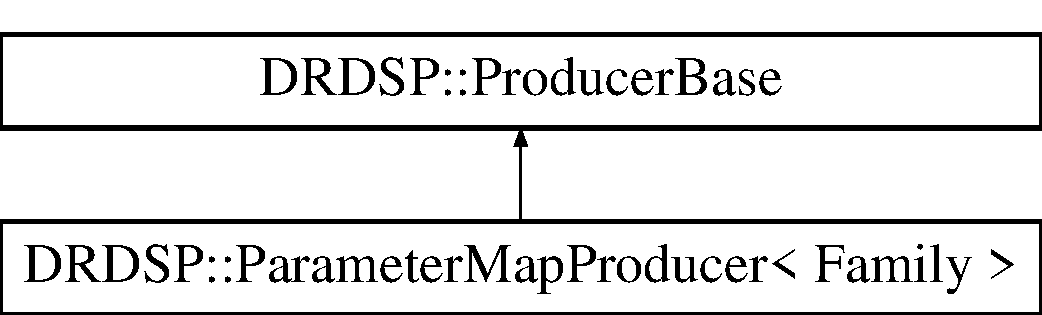
\includegraphics[height=2.000000cm]{struct_d_r_d_s_p_1_1_parameter_map_producer}
\end{center}
\end{figure}
\subsection*{Public Member Functions}
\begin{DoxyCompactItemize}
\item 
\hypertarget{struct_d_r_d_s_p_1_1_parameter_map_producer_a65c2df5b79df0c72c5e2728a5ac5555f}{\hyperlink{struct_d_r_d_s_p_1_1_affine}{Affine\-Xd} {\bfseries Solve\-S\-V\-D} (const \hyperlink{struct_d_r_d_s_p_1_1_family}{Family} \&family, const \hyperlink{struct_d_r_d_s_p_1_1_reduced_data_system}{Reduced\-Data\-System} \&data, const vector$<$ Vector\-Xd $>$ \&parameters)}\label{struct_d_r_d_s_p_1_1_parameter_map_producer_a65c2df5b79df0c72c5e2728a5ac5555f}

\item 
\hypertarget{struct_d_r_d_s_p_1_1_parameter_map_producer_a56b259d4543cf20255e03ce98717fc2c}{\hyperlink{struct_d_r_d_s_p_1_1_affine}{Affine\-Xd} {\bfseries Solve\-Orig} (const \hyperlink{struct_d_r_d_s_p_1_1_family}{Family} \&family, const \hyperlink{struct_d_r_d_s_p_1_1_reduced_data_system}{Reduced\-Data\-System} \&data, const vector$<$ Vector\-Xd $>$ \&parameters)}\label{struct_d_r_d_s_p_1_1_parameter_map_producer_a56b259d4543cf20255e03ce98717fc2c}

\end{DoxyCompactItemize}
\subsection*{Protected Member Functions}
\begin{DoxyCompactItemize}
\item 
\hypertarget{struct_d_r_d_s_p_1_1_parameter_map_producer_a3f9de30fef28ea3f175f734c6f162aae}{void {\bfseries Compute\-Matrices} (Matrix\-Xd \&A, Vector\-Xd \&B, const \hyperlink{struct_d_r_d_s_p_1_1_family}{Family} \&family, const \hyperlink{struct_d_r_d_s_p_1_1_reduced_data}{Reduced\-Data} \&data, const Vector\-Xd \&parameter) const }\label{struct_d_r_d_s_p_1_1_parameter_map_producer_a3f9de30fef28ea3f175f734c6f162aae}

\item 
\hypertarget{struct_d_r_d_s_p_1_1_parameter_map_producer_a71ea46d936b75012e524a305e247b6dd}{Vector\-Xd {\bfseries Compute\-Parameter\-Map} (const \hyperlink{struct_d_r_d_s_p_1_1_family}{Family} \&family, const \hyperlink{struct_d_r_d_s_p_1_1_reduced_data_system}{Reduced\-Data\-System} \&data, const vector$<$ Vector\-Xd $>$ \&parameters)}\label{struct_d_r_d_s_p_1_1_parameter_map_producer_a71ea46d936b75012e524a305e247b6dd}

\end{DoxyCompactItemize}
\subsection*{Static Protected Member Functions}
\begin{DoxyCompactItemize}
\item 
\hypertarget{struct_d_r_d_s_p_1_1_parameter_map_producer_a5efd5118906a3d8e0a84dc927dc95000}{static Matrix\-Xd {\bfseries Compute\-D} (const Vector\-Xd \&parameter, int64\-\_\-t ldim)}\label{struct_d_r_d_s_p_1_1_parameter_map_producer_a5efd5118906a3d8e0a84dc927dc95000}

\end{DoxyCompactItemize}
\subsection*{Additional Inherited Members}


The documentation for this struct was generated from the following file\-:\begin{DoxyCompactItemize}
\item 
include/\-D\-R\-D\-S\-P/dynamics/parameter\-\_\-map\-\_\-producer.\-h\end{DoxyCompactItemize}

\hypertarget{struct_d_r_d_s_p_1_1_p_map_family}{\section{D\-R\-D\-S\-P\-:\-:P\-Map\-Family$<$ F, P\-Map $>$ Struct Template Reference}
\label{struct_d_r_d_s_p_1_1_p_map_family}\index{D\-R\-D\-S\-P\-::\-P\-Map\-Family$<$ F, P\-Map $>$@{D\-R\-D\-S\-P\-::\-P\-Map\-Family$<$ F, P\-Map $>$}}
}


A parameter map applied to a family.  




{\ttfamily \#include $<$model.\-h$>$}

Inheritance diagram for D\-R\-D\-S\-P\-:\-:P\-Map\-Family$<$ F, P\-Map $>$\-:\begin{figure}[H]
\begin{center}
\leavevmode
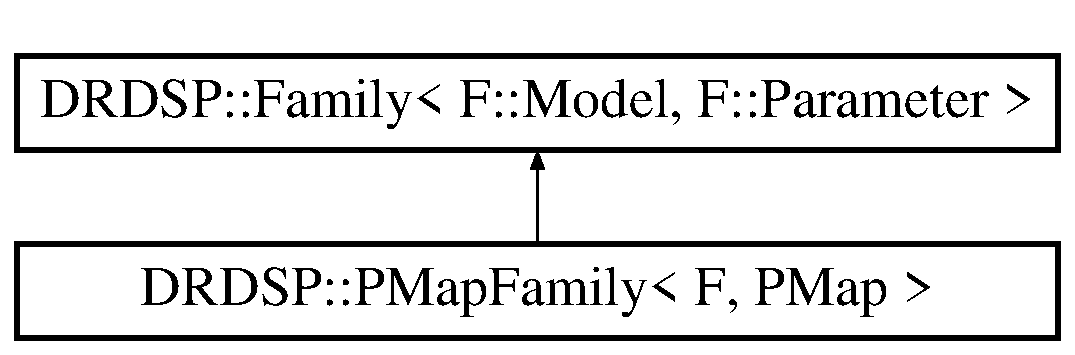
\includegraphics[height=2.000000cm]{struct_d_r_d_s_p_1_1_p_map_family}
\end{center}
\end{figure}
\subsection*{Public Member Functions}
\begin{DoxyCompactItemize}
\item 
\hypertarget{struct_d_r_d_s_p_1_1_p_map_family_a75d942e4c38daaa1b399ececdbb3fb86}{{\bfseries P\-Map\-Family} (const F \&f, const P\-Map \&p)}\label{struct_d_r_d_s_p_1_1_p_map_family_a75d942e4c38daaa1b399ececdbb3fb86}

\item 
\hypertarget{struct_d_r_d_s_p_1_1_p_map_family_a4f852cebd93cf4f45f7a49862846f1bb}{Model {\bfseries operator()} (const Parameter \&parameter) const }\label{struct_d_r_d_s_p_1_1_p_map_family_a4f852cebd93cf4f45f7a49862846f1bb}

\end{DoxyCompactItemize}
\subsection*{Public Attributes}
\begin{DoxyCompactItemize}
\item 
\hypertarget{struct_d_r_d_s_p_1_1_p_map_family_adc9d74d88755b8efa9002560b6f75cb2}{F \hyperlink{struct_d_r_d_s_p_1_1_p_map_family_adc9d74d88755b8efa9002560b6f75cb2}{family}}\label{struct_d_r_d_s_p_1_1_p_map_family_adc9d74d88755b8efa9002560b6f75cb2}

\begin{DoxyCompactList}\small\item\em The underlying family. \end{DoxyCompactList}\item 
\hypertarget{struct_d_r_d_s_p_1_1_p_map_family_a8bd9bac383199f4c35460f5063a13f2b}{P\-Map \hyperlink{struct_d_r_d_s_p_1_1_p_map_family_a8bd9bac383199f4c35460f5063a13f2b}{pmap}}\label{struct_d_r_d_s_p_1_1_p_map_family_a8bd9bac383199f4c35460f5063a13f2b}

\begin{DoxyCompactList}\small\item\em A map between parameter spaces. \end{DoxyCompactList}\end{DoxyCompactItemize}
\subsection*{Additional Inherited Members}


\subsection{Detailed Description}
\subsubsection*{template$<$typename F, typename P\-Map$>$struct D\-R\-D\-S\-P\-::\-P\-Map\-Family$<$ F, P\-Map $>$}

A parameter map applied to a family. 

The documentation for this struct was generated from the following file\-:\begin{DoxyCompactItemize}
\item 
include/\-D\-R\-D\-S\-P/dynamics/model.\-h\end{DoxyCompactItemize}

\hypertarget{struct_d_r_d_s_p_1_1_polyharmonic_spline}{\section{D\-R\-D\-S\-P\-:\-:Polyharmonic\-Spline$<$ N $>$ Struct Template Reference}
\label{struct_d_r_d_s_p_1_1_polyharmonic_spline}\index{D\-R\-D\-S\-P\-::\-Polyharmonic\-Spline$<$ N $>$@{D\-R\-D\-S\-P\-::\-Polyharmonic\-Spline$<$ N $>$}}
}
\subsection*{Public Member Functions}
\begin{DoxyCompactItemize}
\item 
\hypertarget{struct_d_r_d_s_p_1_1_polyharmonic_spline_a2ebd78e3db5b52236072e82e2c276d31}{{\footnotesize template$<$typename T $>$ }\\T {\bfseries operator()} (T r) const }\label{struct_d_r_d_s_p_1_1_polyharmonic_spline_a2ebd78e3db5b52236072e82e2c276d31}

\item 
\hypertarget{struct_d_r_d_s_p_1_1_polyharmonic_spline_aa81c69a1ca35f1d31d9c18abc312ba3e}{{\footnotesize template$<$typename T $>$ }\\T {\bfseries Derivative} (T r) const }\label{struct_d_r_d_s_p_1_1_polyharmonic_spline_aa81c69a1ca35f1d31d9c18abc312ba3e}

\end{DoxyCompactItemize}


The documentation for this struct was generated from the following file\-:\begin{DoxyCompactItemize}
\item 
include/\-D\-R\-D\-S\-P/dynamics/polyharmonic\-\_\-spline.\-h\end{DoxyCompactItemize}

\hypertarget{struct_d_r_d_s_p_1_1_polyharmonic_spline_3_011_01_4}{\section{D\-R\-D\-S\-P\-:\-:Polyharmonic\-Spline$<$ 1 $>$ Struct Template Reference}
\label{struct_d_r_d_s_p_1_1_polyharmonic_spline_3_011_01_4}\index{D\-R\-D\-S\-P\-::\-Polyharmonic\-Spline$<$ 1 $>$@{D\-R\-D\-S\-P\-::\-Polyharmonic\-Spline$<$ 1 $>$}}
}
\subsection*{Public Member Functions}
\begin{DoxyCompactItemize}
\item 
\hypertarget{struct_d_r_d_s_p_1_1_polyharmonic_spline_3_011_01_4_ab969c8592975972909550dd54e09b0b3}{{\footnotesize template$<$typename T $>$ }\\T {\bfseries operator()} (T r) const }\label{struct_d_r_d_s_p_1_1_polyharmonic_spline_3_011_01_4_ab969c8592975972909550dd54e09b0b3}

\item 
\hypertarget{struct_d_r_d_s_p_1_1_polyharmonic_spline_3_011_01_4_a89606285e81214bed46fec44c5ca083f}{{\footnotesize template$<$typename T $>$ }\\T {\bfseries Derivative} (T r) const }\label{struct_d_r_d_s_p_1_1_polyharmonic_spline_3_011_01_4_a89606285e81214bed46fec44c5ca083f}

\end{DoxyCompactItemize}


The documentation for this struct was generated from the following file\-:\begin{DoxyCompactItemize}
\item 
include/\-D\-R\-D\-S\-P/dynamics/polyharmonic\-\_\-spline.\-h\end{DoxyCompactItemize}

\hypertarget{struct_d_r_d_s_p_1_1_polyharmonic_spline_3_012_01_4}{\section{D\-R\-D\-S\-P\-:\-:Polyharmonic\-Spline$<$ 2 $>$ Struct Template Reference}
\label{struct_d_r_d_s_p_1_1_polyharmonic_spline_3_012_01_4}\index{D\-R\-D\-S\-P\-::\-Polyharmonic\-Spline$<$ 2 $>$@{D\-R\-D\-S\-P\-::\-Polyharmonic\-Spline$<$ 2 $>$}}
}
\subsection*{Public Member Functions}
\begin{DoxyCompactItemize}
\item 
\hypertarget{struct_d_r_d_s_p_1_1_polyharmonic_spline_3_012_01_4_ac1903e0b1c7b324e6a61bb1af88fbdf1}{{\footnotesize template$<$typename T $>$ }\\T {\bfseries operator()} (T r) const }\label{struct_d_r_d_s_p_1_1_polyharmonic_spline_3_012_01_4_ac1903e0b1c7b324e6a61bb1af88fbdf1}

\item 
\hypertarget{struct_d_r_d_s_p_1_1_polyharmonic_spline_3_012_01_4_a2d6b76df2c058819ea81984a953cba34}{{\footnotesize template$<$typename T $>$ }\\T {\bfseries Derivative} (T r) const }\label{struct_d_r_d_s_p_1_1_polyharmonic_spline_3_012_01_4_a2d6b76df2c058819ea81984a953cba34}

\end{DoxyCompactItemize}


The documentation for this struct was generated from the following file\-:\begin{DoxyCompactItemize}
\item 
include/\-D\-R\-D\-S\-P/dynamics/polyharmonic\-\_\-spline.\-h\end{DoxyCompactItemize}

\hypertarget{struct_d_r_d_s_p_1_1_polyharmonic_spline_3_013_01_4}{\section{D\-R\-D\-S\-P\-:\-:Polyharmonic\-Spline$<$ 3 $>$ Struct Template Reference}
\label{struct_d_r_d_s_p_1_1_polyharmonic_spline_3_013_01_4}\index{D\-R\-D\-S\-P\-::\-Polyharmonic\-Spline$<$ 3 $>$@{D\-R\-D\-S\-P\-::\-Polyharmonic\-Spline$<$ 3 $>$}}
}
\subsection*{Public Member Functions}
\begin{DoxyCompactItemize}
\item 
\hypertarget{struct_d_r_d_s_p_1_1_polyharmonic_spline_3_013_01_4_ad67a9a1674be8012a4b53c45250da713}{{\footnotesize template$<$typename T $>$ }\\T {\bfseries operator()} (T r) const }\label{struct_d_r_d_s_p_1_1_polyharmonic_spline_3_013_01_4_ad67a9a1674be8012a4b53c45250da713}

\item 
\hypertarget{struct_d_r_d_s_p_1_1_polyharmonic_spline_3_013_01_4_a227b29fdc10b6938a65fbccc21cbc293}{{\footnotesize template$<$typename T $>$ }\\T {\bfseries Derivative} (T r) const }\label{struct_d_r_d_s_p_1_1_polyharmonic_spline_3_013_01_4_a227b29fdc10b6938a65fbccc21cbc293}

\end{DoxyCompactItemize}


The documentation for this struct was generated from the following file\-:\begin{DoxyCompactItemize}
\item 
include/\-D\-R\-D\-S\-P/dynamics/polyharmonic\-\_\-spline.\-h\end{DoxyCompactItemize}

\hypertarget{struct_d_r_d_s_p_1_1_polyharmonic_spline_3_014_01_4}{\section{D\-R\-D\-S\-P\-:\-:Polyharmonic\-Spline$<$ 4 $>$ Struct Template Reference}
\label{struct_d_r_d_s_p_1_1_polyharmonic_spline_3_014_01_4}\index{D\-R\-D\-S\-P\-::\-Polyharmonic\-Spline$<$ 4 $>$@{D\-R\-D\-S\-P\-::\-Polyharmonic\-Spline$<$ 4 $>$}}
}
\subsection*{Public Member Functions}
\begin{DoxyCompactItemize}
\item 
\hypertarget{struct_d_r_d_s_p_1_1_polyharmonic_spline_3_014_01_4_a59308bf407d1523bf4c3a7f42e00b194}{{\footnotesize template$<$typename T $>$ }\\T {\bfseries operator()} (T r) const }\label{struct_d_r_d_s_p_1_1_polyharmonic_spline_3_014_01_4_a59308bf407d1523bf4c3a7f42e00b194}

\item 
\hypertarget{struct_d_r_d_s_p_1_1_polyharmonic_spline_3_014_01_4_ac7ef51f745007e1c1d475a40761ea06c}{{\footnotesize template$<$typename T $>$ }\\T {\bfseries Derivative} (T r) const }\label{struct_d_r_d_s_p_1_1_polyharmonic_spline_3_014_01_4_ac7ef51f745007e1c1d475a40761ea06c}

\end{DoxyCompactItemize}


The documentation for this struct was generated from the following file\-:\begin{DoxyCompactItemize}
\item 
include/\-D\-R\-D\-S\-P/dynamics/polyharmonic\-\_\-spline.\-h\end{DoxyCompactItemize}

\hypertarget{struct_d_r_d_s_p_1_1_polyharmonic_spline_3_015_01_4}{\section{D\-R\-D\-S\-P\-:\-:Polyharmonic\-Spline$<$ 5 $>$ Struct Template Reference}
\label{struct_d_r_d_s_p_1_1_polyharmonic_spline_3_015_01_4}\index{D\-R\-D\-S\-P\-::\-Polyharmonic\-Spline$<$ 5 $>$@{D\-R\-D\-S\-P\-::\-Polyharmonic\-Spline$<$ 5 $>$}}
}
\subsection*{Public Member Functions}
\begin{DoxyCompactItemize}
\item 
\hypertarget{struct_d_r_d_s_p_1_1_polyharmonic_spline_3_015_01_4_abaad8dd3ec1bbf64e233c53a0921bddd}{{\footnotesize template$<$typename T $>$ }\\T {\bfseries operator()} (T r) const }\label{struct_d_r_d_s_p_1_1_polyharmonic_spline_3_015_01_4_abaad8dd3ec1bbf64e233c53a0921bddd}

\item 
\hypertarget{struct_d_r_d_s_p_1_1_polyharmonic_spline_3_015_01_4_a7a40c9529cc0ec4da5ac38c5ea87ee65}{{\footnotesize template$<$typename T $>$ }\\T {\bfseries Derivative} (T r) const }\label{struct_d_r_d_s_p_1_1_polyharmonic_spline_3_015_01_4_a7a40c9529cc0ec4da5ac38c5ea87ee65}

\end{DoxyCompactItemize}


The documentation for this struct was generated from the following file\-:\begin{DoxyCompactItemize}
\item 
include/\-D\-R\-D\-S\-P/dynamics/polyharmonic\-\_\-spline.\-h\end{DoxyCompactItemize}

\hypertarget{struct_d_r_d_s_p_1_1_polyharmonic_spline_3_016_01_4}{\section{D\-R\-D\-S\-P\-:\-:Polyharmonic\-Spline$<$ 6 $>$ Struct Template Reference}
\label{struct_d_r_d_s_p_1_1_polyharmonic_spline_3_016_01_4}\index{D\-R\-D\-S\-P\-::\-Polyharmonic\-Spline$<$ 6 $>$@{D\-R\-D\-S\-P\-::\-Polyharmonic\-Spline$<$ 6 $>$}}
}
\subsection*{Public Member Functions}
\begin{DoxyCompactItemize}
\item 
\hypertarget{struct_d_r_d_s_p_1_1_polyharmonic_spline_3_016_01_4_ae1dd93153178876d0748a26fc2cb3b8e}{{\footnotesize template$<$typename T $>$ }\\T {\bfseries operator()} (T r) const }\label{struct_d_r_d_s_p_1_1_polyharmonic_spline_3_016_01_4_ae1dd93153178876d0748a26fc2cb3b8e}

\item 
\hypertarget{struct_d_r_d_s_p_1_1_polyharmonic_spline_3_016_01_4_ad994c2a115155d2e20a8e2b0af33dd9f}{{\footnotesize template$<$typename T $>$ }\\T {\bfseries Derivative} (T r) const }\label{struct_d_r_d_s_p_1_1_polyharmonic_spline_3_016_01_4_ad994c2a115155d2e20a8e2b0af33dd9f}

\end{DoxyCompactItemize}


The documentation for this struct was generated from the following file\-:\begin{DoxyCompactItemize}
\item 
include/\-D\-R\-D\-S\-P/dynamics/polyharmonic\-\_\-spline.\-h\end{DoxyCompactItemize}

\hypertarget{struct_d_r_d_s_p_1_1_polyharmonic_spline_3_017_01_4}{\section{D\-R\-D\-S\-P\-:\-:Polyharmonic\-Spline$<$ 7 $>$ Struct Template Reference}
\label{struct_d_r_d_s_p_1_1_polyharmonic_spline_3_017_01_4}\index{D\-R\-D\-S\-P\-::\-Polyharmonic\-Spline$<$ 7 $>$@{D\-R\-D\-S\-P\-::\-Polyharmonic\-Spline$<$ 7 $>$}}
}
\subsection*{Public Member Functions}
\begin{DoxyCompactItemize}
\item 
\hypertarget{struct_d_r_d_s_p_1_1_polyharmonic_spline_3_017_01_4_a7c3e3d056498269d5c3ba22311091e7b}{{\footnotesize template$<$typename T $>$ }\\T {\bfseries operator()} (T r) const }\label{struct_d_r_d_s_p_1_1_polyharmonic_spline_3_017_01_4_a7c3e3d056498269d5c3ba22311091e7b}

\item 
\hypertarget{struct_d_r_d_s_p_1_1_polyharmonic_spline_3_017_01_4_af4723f77839c9789889edfbdfb1768d4}{{\footnotesize template$<$typename T $>$ }\\T {\bfseries Derivative} (T r) const }\label{struct_d_r_d_s_p_1_1_polyharmonic_spline_3_017_01_4_af4723f77839c9789889edfbdfb1768d4}

\end{DoxyCompactItemize}


The documentation for this struct was generated from the following file\-:\begin{DoxyCompactItemize}
\item 
include/\-D\-R\-D\-S\-P/dynamics/polyharmonic\-\_\-spline.\-h\end{DoxyCompactItemize}

\hypertarget{struct_d_r_d_s_p_1_1_polyharmonic_spline_3_018_01_4}{\section{D\-R\-D\-S\-P\-:\-:Polyharmonic\-Spline$<$ 8 $>$ Struct Template Reference}
\label{struct_d_r_d_s_p_1_1_polyharmonic_spline_3_018_01_4}\index{D\-R\-D\-S\-P\-::\-Polyharmonic\-Spline$<$ 8 $>$@{D\-R\-D\-S\-P\-::\-Polyharmonic\-Spline$<$ 8 $>$}}
}
\subsection*{Public Member Functions}
\begin{DoxyCompactItemize}
\item 
\hypertarget{struct_d_r_d_s_p_1_1_polyharmonic_spline_3_018_01_4_a30a5d6bb3601f4c3a7b268f30475c5a4}{{\footnotesize template$<$typename T $>$ }\\T {\bfseries operator()} (T r) const }\label{struct_d_r_d_s_p_1_1_polyharmonic_spline_3_018_01_4_a30a5d6bb3601f4c3a7b268f30475c5a4}

\item 
\hypertarget{struct_d_r_d_s_p_1_1_polyharmonic_spline_3_018_01_4_a75a87b5ada7a25992948f19247dae95c}{{\footnotesize template$<$typename T $>$ }\\T {\bfseries Derivative} (T r) const }\label{struct_d_r_d_s_p_1_1_polyharmonic_spline_3_018_01_4_a75a87b5ada7a25992948f19247dae95c}

\end{DoxyCompactItemize}


The documentation for this struct was generated from the following file\-:\begin{DoxyCompactItemize}
\item 
include/\-D\-R\-D\-S\-P/dynamics/polyharmonic\-\_\-spline.\-h\end{DoxyCompactItemize}

\hypertarget{struct_d_r_d_s_p_1_1_producer_base}{\section{D\-R\-D\-S\-P\-:\-:Producer\-Base Struct Reference}
\label{struct_d_r_d_s_p_1_1_producer_base}\index{D\-R\-D\-S\-P\-::\-Producer\-Base@{D\-R\-D\-S\-P\-::\-Producer\-Base}}
}
Inheritance diagram for D\-R\-D\-S\-P\-:\-:Producer\-Base\-:\begin{figure}[H]
\begin{center}
\leavevmode
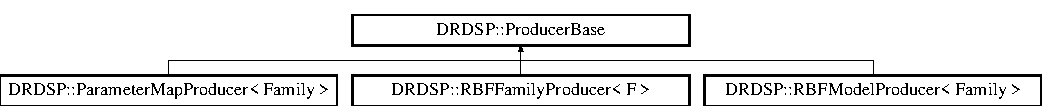
\includegraphics[height=1.408805cm]{struct_d_r_d_s_p_1_1_producer_base}
\end{center}
\end{figure}
\subsection*{Public Member Functions}
\begin{DoxyCompactItemize}
\item 
\hypertarget{struct_d_r_d_s_p_1_1_producer_base_addbb029e21d29fc090c177509d7bcd3f}{{\footnotesize template$<$typename Model $>$ }\\double {\bfseries Compute\-Total\-Cost} (const \hyperlink{struct_d_r_d_s_p_1_1_model}{Model} \&model, const \hyperlink{struct_d_r_d_s_p_1_1_reduced_data}{Reduced\-Data} \&data) const }\label{struct_d_r_d_s_p_1_1_producer_base_addbb029e21d29fc090c177509d7bcd3f}

\item 
\hypertarget{struct_d_r_d_s_p_1_1_producer_base_a3e47c61d879ea97d767641adeecb1ac8}{{\footnotesize template$<$typename Family $>$ }\\double {\bfseries Compute\-Total\-Cost} (const \hyperlink{struct_d_r_d_s_p_1_1_family}{Family} \&family, const \hyperlink{struct_d_r_d_s_p_1_1_reduced_data_system}{Reduced\-Data\-System} \&data, const vector$<$ Vector\-Xd $>$ \&parameters) const }\label{struct_d_r_d_s_p_1_1_producer_base_a3e47c61d879ea97d767641adeecb1ac8}

\end{DoxyCompactItemize}
\subsection*{Public Attributes}
\begin{DoxyCompactItemize}
\item 
\hypertarget{struct_d_r_d_s_p_1_1_producer_base_ac8a769138a797ad3cf75d6280a7163d1}{double {\bfseries fit\-Weight} \mbox{[}2\mbox{]}}\label{struct_d_r_d_s_p_1_1_producer_base_ac8a769138a797ad3cf75d6280a7163d1}

\end{DoxyCompactItemize}


The documentation for this struct was generated from the following file\-:\begin{DoxyCompactItemize}
\item 
include/\-D\-R\-D\-S\-P/dynamics/producer\-\_\-base.\-h\end{DoxyCompactItemize}

\hypertarget{struct_d_r_d_s_p_1_1_proj_p_o_d}{\section{D\-R\-D\-S\-P\-:\-:Proj\-P\-O\-D Struct Reference}
\label{struct_d_r_d_s_p_1_1_proj_p_o_d}\index{D\-R\-D\-S\-P\-::\-Proj\-P\-O\-D@{D\-R\-D\-S\-P\-::\-Proj\-P\-O\-D}}
}
\subsection*{Public Member Functions}
\begin{DoxyCompactItemize}
\item 
\hypertarget{struct_d_r_d_s_p_1_1_proj_p_o_d_aca597efa4efe8a9f3632b4648ab3bee6}{{\bfseries Proj\-P\-O\-D} (uint32\-\_\-t target\-Dimension)}\label{struct_d_r_d_s_p_1_1_proj_p_o_d_aca597efa4efe8a9f3632b4648ab3bee6}

\item 
\hypertarget{struct_d_r_d_s_p_1_1_proj_p_o_d_ad852a4b068691732d2be2b0fc6a50fef}{\hyperlink{struct_d_r_d_s_p_1_1_proj_p_o_d}{Proj\-P\-O\-D} \& {\bfseries Find} (const \hyperlink{struct_d_r_d_s_p_1_1_data_set}{Data\-Set} \&data)}\label{struct_d_r_d_s_p_1_1_proj_p_o_d_ad852a4b068691732d2be2b0fc6a50fef}

\item 
\hypertarget{struct_d_r_d_s_p_1_1_proj_p_o_d_a00d7aa64d9f4c3e396bb37aa2e493747}{\hyperlink{struct_d_r_d_s_p_1_1_proj_p_o_d}{Proj\-P\-O\-D} \& {\bfseries Find} (const \hyperlink{struct_d_r_d_s_p_1_1_data_system}{Data\-System} \&data)}\label{struct_d_r_d_s_p_1_1_proj_p_o_d_a00d7aa64d9f4c3e396bb37aa2e493747}

\item 
\hypertarget{struct_d_r_d_s_p_1_1_proj_p_o_d_a01949683f073d757884e0dc86f9fe26d}{const \hyperlink{struct_d_r_d_s_p_1_1_proj_p_o_d}{Proj\-P\-O\-D} \& {\bfseries Write} (const char $\ast$filename) const }\label{struct_d_r_d_s_p_1_1_proj_p_o_d_a01949683f073d757884e0dc86f9fe26d}

\end{DoxyCompactItemize}
\subsection*{Public Attributes}
\begin{DoxyCompactItemize}
\item 
\hypertarget{struct_d_r_d_s_p_1_1_proj_p_o_d_accfcb1fe9ae69a35a85d74732a04c9c7}{Matrix\-Xd {\bfseries W}}\label{struct_d_r_d_s_p_1_1_proj_p_o_d_accfcb1fe9ae69a35a85d74732a04c9c7}

\item 
\hypertarget{struct_d_r_d_s_p_1_1_proj_p_o_d_acdfe762ff68aa2be10d16797312a8215}{uint32\-\_\-t {\bfseries target\-Dimension} = 2}\label{struct_d_r_d_s_p_1_1_proj_p_o_d_acdfe762ff68aa2be10d16797312a8215}

\end{DoxyCompactItemize}
\subsection*{Protected Attributes}
\begin{DoxyCompactItemize}
\item 
\hypertarget{struct_d_r_d_s_p_1_1_proj_p_o_d_a063bb5fe4abf916c3c7108164de3c5fe}{Jacobi\-S\-V\-D$<$ Matrix\-Xd $>$\\*
\-::Singular\-Values\-Type {\bfseries singular\-Values}}\label{struct_d_r_d_s_p_1_1_proj_p_o_d_a063bb5fe4abf916c3c7108164de3c5fe}

\end{DoxyCompactItemize}


The documentation for this struct was generated from the following files\-:\begin{DoxyCompactItemize}
\item 
include/\-D\-R\-D\-S\-P/projection/proj\-\_\-pod.\-h\item 
src/projection/proj\-\_\-pod.\-cpp\end{DoxyCompactItemize}

\hypertarget{struct_d_r_d_s_p_1_1_proj_secant}{\section{D\-R\-D\-S\-P\-:\-:Proj\-Secant Struct Reference}
\label{struct_d_r_d_s_p_1_1_proj_secant}\index{D\-R\-D\-S\-P\-::\-Proj\-Secant@{D\-R\-D\-S\-P\-::\-Proj\-Secant}}
}
\subsection*{Public Member Functions}
\begin{DoxyCompactItemize}
\item 
\hypertarget{struct_d_r_d_s_p_1_1_proj_secant_a6b9225aa855d0379f792542de6a9f074}{{\bfseries Proj\-Secant} (uint32\-\_\-t target\-Dimension)}\label{struct_d_r_d_s_p_1_1_proj_secant_a6b9225aa855d0379f792542de6a9f074}

\item 
\hypertarget{struct_d_r_d_s_p_1_1_proj_secant_aa55fa8720a3fc21364865b8a7939ab57}{\hyperlink{struct_d_r_d_s_p_1_1_proj_secant}{Proj\-Secant} \& {\bfseries Compute\-Initial} (const \hyperlink{struct_d_r_d_s_p_1_1_data_set}{Data\-Set} \&data)}\label{struct_d_r_d_s_p_1_1_proj_secant_aa55fa8720a3fc21364865b8a7939ab57}

\item 
\hypertarget{struct_d_r_d_s_p_1_1_proj_secant_aa6efb6dce18044a7284965904b1ac755}{\hyperlink{struct_d_r_d_s_p_1_1_proj_secant}{Proj\-Secant} \& {\bfseries Compute\-Initial} (const \hyperlink{struct_d_r_d_s_p_1_1_data_system}{Data\-System} \&data)}\label{struct_d_r_d_s_p_1_1_proj_secant_aa6efb6dce18044a7284965904b1ac755}

\item 
\hypertarget{struct_d_r_d_s_p_1_1_proj_secant_a1b4b5d140093eab8a0313a035ad35f7a}{\hyperlink{struct_d_r_d_s_p_1_1_proj_secant}{Proj\-Secant} \& {\bfseries Find} (const \hyperlink{struct_d_r_d_s_p_1_1_secants}{Secants} \&secants)}\label{struct_d_r_d_s_p_1_1_proj_secant_a1b4b5d140093eab8a0313a035ad35f7a}

\item 
\hypertarget{struct_d_r_d_s_p_1_1_proj_secant_ad6422b7edf25dec73c435bbbc83179d2}{\hyperlink{struct_d_r_d_s_p_1_1_proj_secant}{Proj\-Secant} \& {\bfseries Find} (const \hyperlink{struct_d_r_d_s_p_1_1_secants}{Secants} $\ast$secants, size\-\_\-t N)}\label{struct_d_r_d_s_p_1_1_proj_secant_ad6422b7edf25dec73c435bbbc83179d2}

\item 
\hypertarget{struct_d_r_d_s_p_1_1_proj_secant_af6176307efdb61f11ba39aa8bd155322}{\hyperlink{struct_d_r_d_s_p_1_1_proj_secant}{Proj\-Secant} \& {\bfseries Find} (const vector$<$ \hyperlink{struct_d_r_d_s_p_1_1_secants}{Secants} $>$ \&secants)}\label{struct_d_r_d_s_p_1_1_proj_secant_af6176307efdb61f11ba39aa8bd155322}

\item 
\hypertarget{struct_d_r_d_s_p_1_1_proj_secant_a4c12f28ba578c22c206b0d92ad6eb490}{const \hyperlink{struct_d_r_d_s_p_1_1_proj_secant}{Proj\-Secant} \& {\bfseries Analyse\-Secants} (const \hyperlink{struct_d_r_d_s_p_1_1_secants}{Secants} \&secants) const }\label{struct_d_r_d_s_p_1_1_proj_secant_a4c12f28ba578c22c206b0d92ad6eb490}

\item 
\hypertarget{struct_d_r_d_s_p_1_1_proj_secant_a314a6742c209f41d347eaf652db24761}{const \hyperlink{struct_d_r_d_s_p_1_1_proj_secant}{Proj\-Secant} \& {\bfseries Analyse\-Secants} (const vector$<$ \hyperlink{struct_d_r_d_s_p_1_1_secants}{Secants} $>$ \&secants) const }\label{struct_d_r_d_s_p_1_1_proj_secant_a314a6742c209f41d347eaf652db24761}

\item 
\hypertarget{struct_d_r_d_s_p_1_1_proj_secant_a1b8c61ea307a758c789ae424cd72006c}{const \hyperlink{struct_d_r_d_s_p_1_1_proj_secant}{Proj\-Secant} \& {\bfseries Write\-C\-S\-V} (const char $\ast$filename) const }\label{struct_d_r_d_s_p_1_1_proj_secant_a1b8c61ea307a758c789ae424cd72006c}

\item 
\hypertarget{struct_d_r_d_s_p_1_1_proj_secant_afbb9d6b0aa69ba44619363a69d7f7cef}{const \hyperlink{struct_d_r_d_s_p_1_1_proj_secant}{Proj\-Secant} \& {\bfseries Write\-Binary} (const char $\ast$filename) const }\label{struct_d_r_d_s_p_1_1_proj_secant_afbb9d6b0aa69ba44619363a69d7f7cef}

\item 
\hypertarget{struct_d_r_d_s_p_1_1_proj_secant_ae37dfe0f561f61c3ecfda5abc02e8b25}{bool {\bfseries Read\-Binary} (const char $\ast$filename)}\label{struct_d_r_d_s_p_1_1_proj_secant_ae37dfe0f561f61c3ecfda5abc02e8b25}

\end{DoxyCompactItemize}
\subsection*{Public Attributes}
\begin{DoxyCompactItemize}
\item 
\hypertarget{struct_d_r_d_s_p_1_1_proj_secant_a99ab0daf8cb539f9ecf07132d3994357}{Matrix\-Xd {\bfseries W}}\label{struct_d_r_d_s_p_1_1_proj_secant_a99ab0daf8cb539f9ecf07132d3994357}

\item 
\hypertarget{struct_d_r_d_s_p_1_1_proj_secant_a422dde54e49a8b5ab4f631fc0b8cf829}{double {\bfseries target\-Min\-Projected\-Length} = 0.\-5}\label{struct_d_r_d_s_p_1_1_proj_secant_a422dde54e49a8b5ab4f631fc0b8cf829}

\item 
\hypertarget{struct_d_r_d_s_p_1_1_proj_secant_aa74d47b541db9bf256f9602e2ae0646a}{uint32\-\_\-t {\bfseries target\-Dimension} = 2}\label{struct_d_r_d_s_p_1_1_proj_secant_aa74d47b541db9bf256f9602e2ae0646a}

\item 
\hypertarget{struct_d_r_d_s_p_1_1_proj_secant_afa9954dc50be3af121c7590879782afa}{uint32\-\_\-t {\bfseries max\-Iterations} = 100}\label{struct_d_r_d_s_p_1_1_proj_secant_afa9954dc50be3af121c7590879782afa}

\end{DoxyCompactItemize}


The documentation for this struct was generated from the following files\-:\begin{DoxyCompactItemize}
\item 
include/\-D\-R\-D\-S\-P/projection/proj\-\_\-secant.\-h\item 
src/projection/proj\-\_\-secant.\-cpp\end{DoxyCompactItemize}

\hypertarget{struct_d_r_d_s_p_1_1_radians}{\section{D\-R\-D\-S\-P\-:\-:Radians$<$ T $>$ Struct Template Reference}
\label{struct_d_r_d_s_p_1_1_radians}\index{D\-R\-D\-S\-P\-::\-Radians$<$ T $>$@{D\-R\-D\-S\-P\-::\-Radians$<$ T $>$}}
}
\subsection*{Public Member Functions}
\begin{DoxyCompactItemize}
\item 
\hypertarget{struct_d_r_d_s_p_1_1_radians_a6d205398a16b398bb1c8025275247e83}{{\bfseries Radians} (T rhs)}\label{struct_d_r_d_s_p_1_1_radians_a6d205398a16b398bb1c8025275247e83}

\item 
\hypertarget{struct_d_r_d_s_p_1_1_radians_a271028672fbaf15e81300554dd983cbf}{{\bfseries Radians} (const \hyperlink{struct_d_r_d_s_p_1_1_degrees}{Degrees}$<$ T $>$ \&rhs)}\label{struct_d_r_d_s_p_1_1_radians_a271028672fbaf15e81300554dd983cbf}

\item 
\hypertarget{struct_d_r_d_s_p_1_1_radians_a88f574f0304ddb62637098b9e1c25eca}{\hyperlink{struct_d_r_d_s_p_1_1_radians}{Radians}$<$ T $>$ \& {\bfseries operator=} (const \hyperlink{struct_d_r_d_s_p_1_1_degrees}{Degrees}$<$ T $>$ \&rhs)}\label{struct_d_r_d_s_p_1_1_radians_a88f574f0304ddb62637098b9e1c25eca}

\item 
\hypertarget{struct_d_r_d_s_p_1_1_radians_a05111a27c968befc781af04b10028e22}{\hyperlink{struct_d_r_d_s_p_1_1_radians}{Radians}$<$ T $>$ {\bfseries operator+} (const \hyperlink{struct_d_r_d_s_p_1_1_radians}{Radians}$<$ T $>$ \&rhs) const }\label{struct_d_r_d_s_p_1_1_radians_a05111a27c968befc781af04b10028e22}

\item 
\hypertarget{struct_d_r_d_s_p_1_1_radians_a8c01c8f0c6551790d85e30cda27c3a95}{\hyperlink{struct_d_r_d_s_p_1_1_radians}{Radians}$<$ T $>$ {\bfseries operator-\/} (const \hyperlink{struct_d_r_d_s_p_1_1_radians}{Radians}$<$ T $>$ \&rhs) const }\label{struct_d_r_d_s_p_1_1_radians_a8c01c8f0c6551790d85e30cda27c3a95}

\item 
\hypertarget{struct_d_r_d_s_p_1_1_radians_ab9da690d7b68008ca17e05b2e6963715}{\hyperlink{struct_d_r_d_s_p_1_1_radians}{Radians}$<$ T $>$ {\bfseries operator$\ast$} (T x) const }\label{struct_d_r_d_s_p_1_1_radians_ab9da690d7b68008ca17e05b2e6963715}

\item 
\hypertarget{struct_d_r_d_s_p_1_1_radians_a07897047e80809903de2b24a75ef534c}{\hyperlink{struct_d_r_d_s_p_1_1_radians}{Radians}$<$ T $>$ {\bfseries operator/} (T x) const }\label{struct_d_r_d_s_p_1_1_radians_a07897047e80809903de2b24a75ef534c}

\item 
\hypertarget{struct_d_r_d_s_p_1_1_radians_aafb763fa3a5204f28198b920506e13c2}{\hyperlink{struct_d_r_d_s_p_1_1_radians}{Radians}$<$ T $>$ \& {\bfseries operator+=} (const \hyperlink{struct_d_r_d_s_p_1_1_radians}{Radians}$<$ T $>$ \&rhs)}\label{struct_d_r_d_s_p_1_1_radians_aafb763fa3a5204f28198b920506e13c2}

\item 
\hypertarget{struct_d_r_d_s_p_1_1_radians_a81751685fa9f9ee094e1ee68296693c3}{\hyperlink{struct_d_r_d_s_p_1_1_radians}{Radians}$<$ T $>$ \& {\bfseries operator-\/=} (const \hyperlink{struct_d_r_d_s_p_1_1_radians}{Radians}$<$ T $>$ \&rhs)}\label{struct_d_r_d_s_p_1_1_radians_a81751685fa9f9ee094e1ee68296693c3}

\item 
\hypertarget{struct_d_r_d_s_p_1_1_radians_aaf111110248993e900a35cad2c26d9c4}{\hyperlink{struct_d_r_d_s_p_1_1_radians}{Radians}$<$ T $>$ \& {\bfseries operator$\ast$=} (T x)}\label{struct_d_r_d_s_p_1_1_radians_aaf111110248993e900a35cad2c26d9c4}

\item 
\hypertarget{struct_d_r_d_s_p_1_1_radians_ad740acd1a6c5be95b62aeb2fcf51d06e}{\hyperlink{struct_d_r_d_s_p_1_1_radians}{Radians}$<$ T $>$ \& {\bfseries operator/=} (T x)}\label{struct_d_r_d_s_p_1_1_radians_ad740acd1a6c5be95b62aeb2fcf51d06e}

\item 
\hypertarget{struct_d_r_d_s_p_1_1_radians_a3beb59d32f418293be14c0b62bc6dff5}{\hyperlink{struct_d_r_d_s_p_1_1_radians}{Radians}$<$ T $>$ {\bfseries operator-\/} () const }\label{struct_d_r_d_s_p_1_1_radians_a3beb59d32f418293be14c0b62bc6dff5}

\item 
\hypertarget{struct_d_r_d_s_p_1_1_radians_a99d53743213f21ea8397cd656195f0df}{bool {\bfseries operator$>$} (const \hyperlink{struct_d_r_d_s_p_1_1_radians}{Radians}$<$ T $>$ \&rhs) const }\label{struct_d_r_d_s_p_1_1_radians_a99d53743213f21ea8397cd656195f0df}

\item 
\hypertarget{struct_d_r_d_s_p_1_1_radians_aa21d804fafb91bbf4496ef08812c9a30}{bool {\bfseries operator$<$} (const \hyperlink{struct_d_r_d_s_p_1_1_radians}{Radians}$<$ T $>$ \&rhs) const }\label{struct_d_r_d_s_p_1_1_radians_aa21d804fafb91bbf4496ef08812c9a30}

\item 
\hypertarget{struct_d_r_d_s_p_1_1_radians_aed74f8e6d3695c060acbbe3ce0a0d69e}{bool {\bfseries operator$>$=} (const \hyperlink{struct_d_r_d_s_p_1_1_radians}{Radians}$<$ T $>$ \&rhs) const }\label{struct_d_r_d_s_p_1_1_radians_aed74f8e6d3695c060acbbe3ce0a0d69e}

\item 
\hypertarget{struct_d_r_d_s_p_1_1_radians_a26075dcaba03a2319b9dd5988627932d}{bool {\bfseries operator$<$=} (const \hyperlink{struct_d_r_d_s_p_1_1_radians}{Radians}$<$ T $>$ \&rhs) const }\label{struct_d_r_d_s_p_1_1_radians_a26075dcaba03a2319b9dd5988627932d}

\item 
\hypertarget{struct_d_r_d_s_p_1_1_radians_a9bcf9fb721967c7f7dfffa36fbf9c820}{{\bfseries operator T} () const }\label{struct_d_r_d_s_p_1_1_radians_a9bcf9fb721967c7f7dfffa36fbf9c820}

\end{DoxyCompactItemize}
\subsection*{Public Attributes}
\begin{DoxyCompactItemize}
\item 
\hypertarget{struct_d_r_d_s_p_1_1_radians_a2de5e1b363f364e72f293bd300e5efbf}{T {\bfseries value}}\label{struct_d_r_d_s_p_1_1_radians_a2de5e1b363f364e72f293bd300e5efbf}

\end{DoxyCompactItemize}


The documentation for this struct was generated from the following file\-:\begin{DoxyCompactItemize}
\item 
include/\-D\-R\-D\-S\-P/geometry/angle.\-h\end{DoxyCompactItemize}

\hypertarget{struct_d_r_d_s_p_1_1_r_b_f}{\section{D\-R\-D\-S\-P\-:\-:R\-B\-F$<$ F $>$ Struct Template Reference}
\label{struct_d_r_d_s_p_1_1_r_b_f}\index{D\-R\-D\-S\-P\-::\-R\-B\-F$<$ F $>$@{D\-R\-D\-S\-P\-::\-R\-B\-F$<$ F $>$}}
}
\subsection*{Public Types}
\begin{DoxyCompactItemize}
\item 
\hypertarget{struct_d_r_d_s_p_1_1_r_b_f_a00ab98fe7441b683d5b9230650d0210f}{typedef F {\bfseries Radial\-Type}}\label{struct_d_r_d_s_p_1_1_r_b_f_a00ab98fe7441b683d5b9230650d0210f}

\end{DoxyCompactItemize}
\subsection*{Public Member Functions}
\begin{DoxyCompactItemize}
\item 
\hypertarget{struct_d_r_d_s_p_1_1_r_b_f_a292acb1f027729dccad15e3e5a1fe5b8}{{\bfseries R\-B\-F} (const F \&f)}\label{struct_d_r_d_s_p_1_1_r_b_f_a292acb1f027729dccad15e3e5a1fe5b8}

\item 
\hypertarget{struct_d_r_d_s_p_1_1_r_b_f_a3ca26fb2fdb36f5361b15a7b1e8f4ef3}{Vector\-Xd {\bfseries operator()} (const Vector\-Xd \&x) const }\label{struct_d_r_d_s_p_1_1_r_b_f_a3ca26fb2fdb36f5361b15a7b1e8f4ef3}

\item 
\hypertarget{struct_d_r_d_s_p_1_1_r_b_f_a68fd3bbc2d3ce97a06205b16e9041aad}{Matrix\-Xd {\bfseries Derivative} (const Vector\-Xd \&x) const }\label{struct_d_r_d_s_p_1_1_r_b_f_a68fd3bbc2d3ce97a06205b16e9041aad}

\item 
\hypertarget{struct_d_r_d_s_p_1_1_r_b_f_a1f943d60c73f695e2891a071bc805b09}{Matrix\-Xd {\bfseries Linear\-Weight} (const Vector\-Xd \&x) const }\label{struct_d_r_d_s_p_1_1_r_b_f_a1f943d60c73f695e2891a071bc805b09}

\item 
\hypertarget{struct_d_r_d_s_p_1_1_r_b_f_ac48c6056d1804dec0a951b4806ae3bca}{Matrix\-Xd {\bfseries Linear\-Derivative\-Weight} (const Vector\-Xd \&x) const }\label{struct_d_r_d_s_p_1_1_r_b_f_ac48c6056d1804dec0a951b4806ae3bca}

\end{DoxyCompactItemize}
\subsection*{Public Attributes}
\begin{DoxyCompactItemize}
\item 
\hypertarget{struct_d_r_d_s_p_1_1_r_b_f_a2d46e96d11e49da8ec3e26a9599c7fcd}{Vector\-Xd {\bfseries weight}}\label{struct_d_r_d_s_p_1_1_r_b_f_a2d46e96d11e49da8ec3e26a9599c7fcd}

\item 
\hypertarget{struct_d_r_d_s_p_1_1_r_b_f_ae5e66e28a34f5091aa31fbcb2ba9b14d}{Vector\-Xd {\bfseries centre}}\label{struct_d_r_d_s_p_1_1_r_b_f_ae5e66e28a34f5091aa31fbcb2ba9b14d}

\item 
\hypertarget{struct_d_r_d_s_p_1_1_r_b_f_ae82f9a1e47f6203e58b62864fa85288a}{F {\bfseries func}}\label{struct_d_r_d_s_p_1_1_r_b_f_ae82f9a1e47f6203e58b62864fa85288a}

\end{DoxyCompactItemize}


The documentation for this struct was generated from the following file\-:\begin{DoxyCompactItemize}
\item 
include/\-D\-R\-D\-S\-P/dynamics/radial\-\_\-basis.\-h\end{DoxyCompactItemize}

\hypertarget{struct_d_r_d_s_p_1_1_r_b_f_family}{\section{D\-R\-D\-S\-P\-:\-:R\-B\-F\-Family$<$ F $>$ Struct Template Reference}
\label{struct_d_r_d_s_p_1_1_r_b_f_family}\index{D\-R\-D\-S\-P\-::\-R\-B\-F\-Family$<$ F $>$@{D\-R\-D\-S\-P\-::\-R\-B\-F\-Family$<$ F $>$}}
}
Inheritance diagram for D\-R\-D\-S\-P\-:\-:R\-B\-F\-Family$<$ F $>$\-:\begin{figure}[H]
\begin{center}
\leavevmode
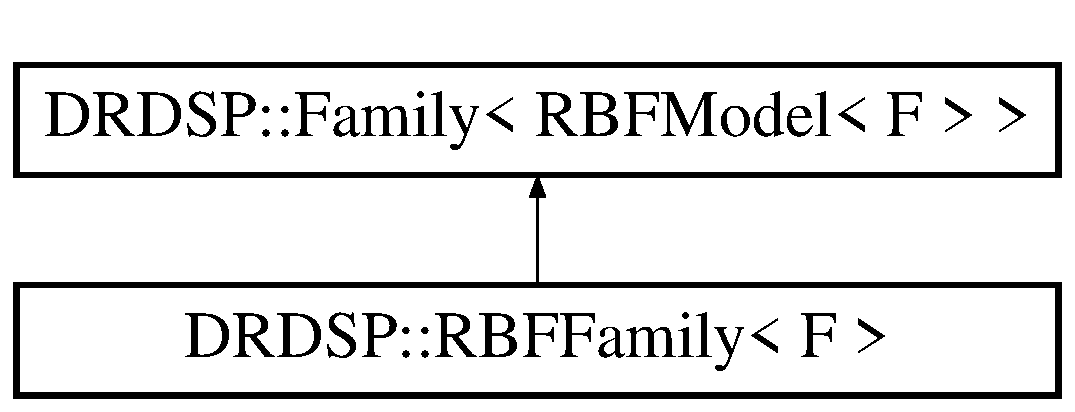
\includegraphics[height=2.000000cm]{struct_d_r_d_s_p_1_1_r_b_f_family}
\end{center}
\end{figure}
\subsection*{Public Member Functions}
\begin{DoxyCompactItemize}
\item 
\hypertarget{struct_d_r_d_s_p_1_1_r_b_f_family_aa74d19e809c115443201acfc23dffcfd}{{\bfseries R\-B\-F\-Family} (uint32\-\_\-t dim, uint32\-\_\-t param\-Dim, uint32\-\_\-t n\-R\-B\-Fs)}\label{struct_d_r_d_s_p_1_1_r_b_f_family_aa74d19e809c115443201acfc23dffcfd}

\item 
\hypertarget{struct_d_r_d_s_p_1_1_r_b_f_family_a910e425f87aec3f906d8ea69e1184317}{\hyperlink{struct_d_r_d_s_p_1_1_r_b_f_model}{R\-B\-F\-Model}$<$ F $>$ {\bfseries operator()} (const Vector\-Xd \&parameter) const }\label{struct_d_r_d_s_p_1_1_r_b_f_family_a910e425f87aec3f906d8ea69e1184317}

\item 
\hypertarget{struct_d_r_d_s_p_1_1_r_b_f_family_a627bffdebc3fe07744c8356d2a0d7b77}{Vector\-Xd {\bfseries Vector\-Field} (const Vector\-Xd \&x, const Vector\-Xd \&parameter)}\label{struct_d_r_d_s_p_1_1_r_b_f_family_a627bffdebc3fe07744c8356d2a0d7b77}

\item 
\hypertarget{struct_d_r_d_s_p_1_1_r_b_f_family_a0f1ab2caec6cfd205773aed2346856ed}{Matrix\-Xd {\bfseries Partials} (const Vector\-Xd \&x, const Vector\-Xd \&parameter)}\label{struct_d_r_d_s_p_1_1_r_b_f_family_a0f1ab2caec6cfd205773aed2346856ed}

\item 
\hypertarget{struct_d_r_d_s_p_1_1_r_b_f_family_a736037a90475af4e332675be367e14c8}{void {\bfseries Write\-C\-S\-V} (const char $\ast$filename) const }\label{struct_d_r_d_s_p_1_1_r_b_f_family_a736037a90475af4e332675be367e14c8}

\item 
\hypertarget{struct_d_r_d_s_p_1_1_r_b_f_family_aac8af8a4b41acb5c51d43ec9500df5c7}{void {\bfseries Read\-Text} (const char $\ast$filename)}\label{struct_d_r_d_s_p_1_1_r_b_f_family_aac8af8a4b41acb5c51d43ec9500df5c7}

\end{DoxyCompactItemize}
\subsection*{Public Attributes}
\begin{DoxyCompactItemize}
\item 
\hypertarget{struct_d_r_d_s_p_1_1_r_b_f_family_a9ddb0a2cd7e34a292e8f46f5b09b82c6}{\hyperlink{struct_d_r_d_s_p_1_1_affine_parameter_map}{Affine\-Parameter\-Map} {\bfseries affine}}\label{struct_d_r_d_s_p_1_1_r_b_f_family_a9ddb0a2cd7e34a292e8f46f5b09b82c6}

\item 
\hypertarget{struct_d_r_d_s_p_1_1_r_b_f_family_ad84edb55f9f9cca4ebc0f6e63e065919}{\hyperlink{struct_d_r_d_s_p_1_1_r_b_f_model}{R\-B\-F\-Model}$<$ F $>$ {\bfseries model}}\label{struct_d_r_d_s_p_1_1_r_b_f_family_ad84edb55f9f9cca4ebc0f6e63e065919}

\end{DoxyCompactItemize}
\subsection*{Additional Inherited Members}


The documentation for this struct was generated from the following file\-:\begin{DoxyCompactItemize}
\item 
include/\-D\-R\-D\-S\-P/dynamics/rbf\-\_\-family.\-h\end{DoxyCompactItemize}

\hypertarget{struct_d_r_d_s_p_1_1_r_b_f_family_producer}{\section{D\-R\-D\-S\-P\-:\-:R\-B\-F\-Family\-Producer$<$ F $>$ Struct Template Reference}
\label{struct_d_r_d_s_p_1_1_r_b_f_family_producer}\index{D\-R\-D\-S\-P\-::\-R\-B\-F\-Family\-Producer$<$ F $>$@{D\-R\-D\-S\-P\-::\-R\-B\-F\-Family\-Producer$<$ F $>$}}
}
Inheritance diagram for D\-R\-D\-S\-P\-:\-:R\-B\-F\-Family\-Producer$<$ F $>$\-:\begin{figure}[H]
\begin{center}
\leavevmode
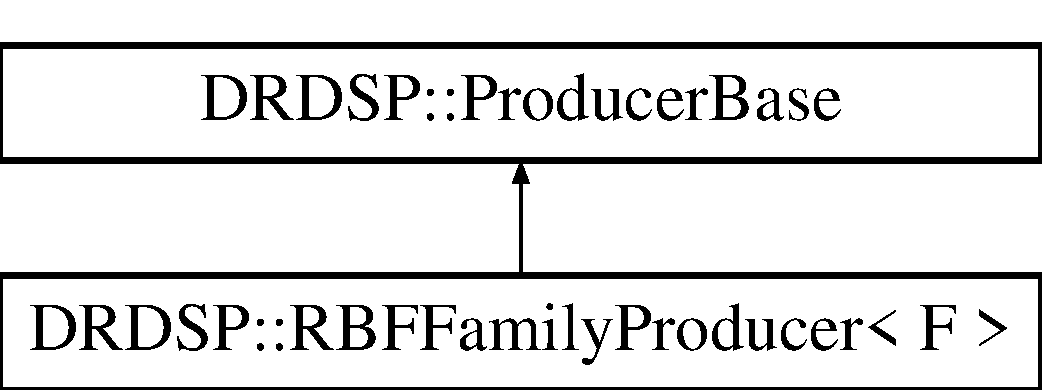
\includegraphics[height=2.000000cm]{struct_d_r_d_s_p_1_1_r_b_f_family_producer}
\end{center}
\end{figure}
\subsection*{Public Types}
\begin{DoxyCompactItemize}
\item 
\hypertarget{struct_d_r_d_s_p_1_1_r_b_f_family_producer_adeef9e5c4bb8e84b47d6975b5fd0b9a5}{typedef \hyperlink{struct_d_r_d_s_p_1_1_p_map_family}{P\-Map\-Family}$<$ \hyperlink{struct_d_r_d_s_p_1_1_r_b_f_family}{R\-B\-F\-Family}\\*
$<$ F $>$, \hyperlink{struct_d_r_d_s_p_1_1_affine}{Affine\-Xd} $>$ {\bfseries Reduced\-Family}}\label{struct_d_r_d_s_p_1_1_r_b_f_family_producer_adeef9e5c4bb8e84b47d6975b5fd0b9a5}

\end{DoxyCompactItemize}
\subsection*{Public Member Functions}
\begin{DoxyCompactItemize}
\item 
\hypertarget{struct_d_r_d_s_p_1_1_r_b_f_family_producer_a0282e37f5ef5428167e10724710c20e7}{{\bfseries R\-B\-F\-Family\-Producer} (uint32\-\_\-t n\-R\-B\-Fs)}\label{struct_d_r_d_s_p_1_1_r_b_f_family_producer_a0282e37f5ef5428167e10724710c20e7}

\item 
\hypertarget{struct_d_r_d_s_p_1_1_r_b_f_family_producer_a6e1dcce56a93b0504c2b1c4d36cc7ff3}{\hyperlink{struct_d_r_d_s_p_1_1_p_map_family}{Reduced\-Family} {\bfseries Brute\-Force} (const \hyperlink{struct_d_r_d_s_p_1_1_reduced_data_system}{Reduced\-Data\-System} \&data, const vector$<$ Vector\-Xd $>$ \&parameters, uint32\-\_\-t num\-Iterations) const }\label{struct_d_r_d_s_p_1_1_r_b_f_family_producer_a6e1dcce56a93b0504c2b1c4d36cc7ff3}

\item 
\hypertarget{struct_d_r_d_s_p_1_1_r_b_f_family_producer_af58f8bd5bdcd8730766c1bc186f4372c}{\hyperlink{struct_d_r_d_s_p_1_1_p_map_family}{Reduced\-Family} {\bfseries Brute\-Force} (const \hyperlink{struct_d_r_d_s_p_1_1_reduced_data_system}{Reduced\-Data\-System} \&data, const vector$<$ Vector\-Xd $>$ \&parameters, uint32\-\_\-t num\-Iterations, uint32\-\_\-t num\-Threads) const }\label{struct_d_r_d_s_p_1_1_r_b_f_family_producer_af58f8bd5bdcd8730766c1bc186f4372c}

\end{DoxyCompactItemize}
\subsection*{Public Attributes}
\begin{DoxyCompactItemize}
\item 
\hypertarget{struct_d_r_d_s_p_1_1_r_b_f_family_producer_a83431f5c3b6616def3277dbc57fe412b}{double {\bfseries box\-Scale}}\label{struct_d_r_d_s_p_1_1_r_b_f_family_producer_a83431f5c3b6616def3277dbc57fe412b}

\item 
\hypertarget{struct_d_r_d_s_p_1_1_r_b_f_family_producer_ad65e12c9e040fba915381b0af0031b21}{uint32\-\_\-t {\bfseries num\-R\-B\-Fs}}\label{struct_d_r_d_s_p_1_1_r_b_f_family_producer_ad65e12c9e040fba915381b0af0031b21}

\end{DoxyCompactItemize}
\subsection*{Protected Member Functions}
\begin{DoxyCompactItemize}
\item 
\hypertarget{struct_d_r_d_s_p_1_1_r_b_f_family_producer_a1163c5bef56c9fa9e578fa13aaaad329}{\hyperlink{struct_d_r_d_s_p_1_1_p_map_family}{Reduced\-Family} {\bfseries Brute\-Force} (const \hyperlink{struct_d_r_d_s_p_1_1_reduced_data_system}{Reduced\-Data\-System} \&data, const \hyperlink{struct_d_r_d_s_p_1_1_a_a_b_b}{A\-A\-B\-B} \&box, const vector$<$ Vector\-Xd $>$ \&parameters, uint32\-\_\-t seed, uint32\-\_\-t num\-Iterations) const }\label{struct_d_r_d_s_p_1_1_r_b_f_family_producer_a1163c5bef56c9fa9e578fa13aaaad329}

\end{DoxyCompactItemize}


The documentation for this struct was generated from the following file\-:\begin{DoxyCompactItemize}
\item 
include/\-D\-R\-D\-S\-P/dynamics/rbf\-\_\-family\-\_\-producer.\-h\end{DoxyCompactItemize}

\hypertarget{struct_d_r_d_s_p_1_1_r_b_f_model}{\section{D\-R\-D\-S\-P\-:\-:R\-B\-F\-Model$<$ F $>$ Struct Template Reference}
\label{struct_d_r_d_s_p_1_1_r_b_f_model}\index{D\-R\-D\-S\-P\-::\-R\-B\-F\-Model$<$ F $>$@{D\-R\-D\-S\-P\-::\-R\-B\-F\-Model$<$ F $>$}}
}
Inheritance diagram for D\-R\-D\-S\-P\-:\-:R\-B\-F\-Model$<$ F $>$\-:\begin{figure}[H]
\begin{center}
\leavevmode
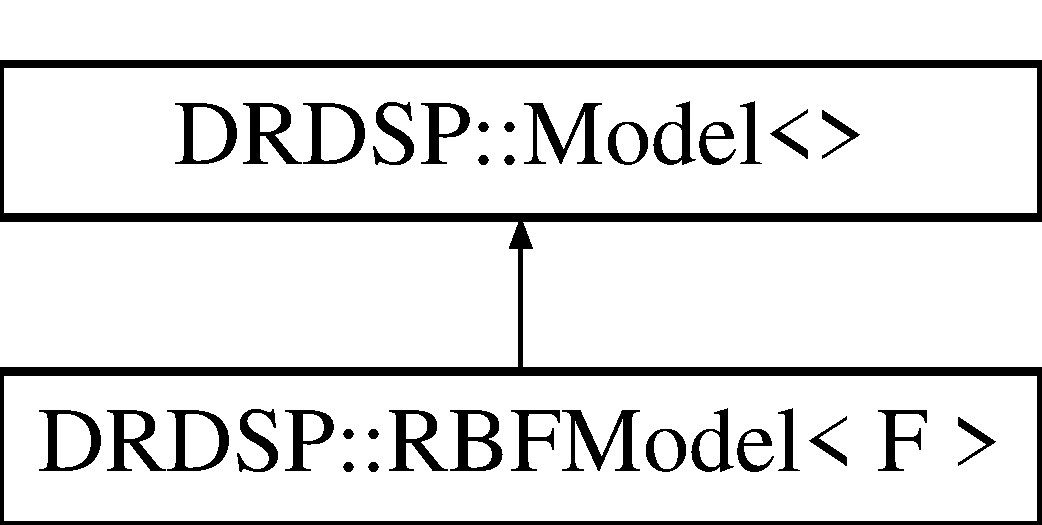
\includegraphics[height=2.000000cm]{struct_d_r_d_s_p_1_1_r_b_f_model}
\end{center}
\end{figure}
\subsection*{Public Member Functions}
\begin{DoxyCompactItemize}
\item 
\hypertarget{struct_d_r_d_s_p_1_1_r_b_f_model_a3f1cbdc52c3439d9936f1703950eb275}{{\bfseries R\-B\-F\-Model} (uint32\-\_\-t dim, uint32\-\_\-t n\-R\-B\-Fs)}\label{struct_d_r_d_s_p_1_1_r_b_f_model_a3f1cbdc52c3439d9936f1703950eb275}

\item 
\hypertarget{struct_d_r_d_s_p_1_1_r_b_f_model_a097398c265c5a82ee0d948dcc26575b6}{Vector\-Xd {\bfseries operator()} (const Vector\-Xd \&x) const }\label{struct_d_r_d_s_p_1_1_r_b_f_model_a097398c265c5a82ee0d948dcc26575b6}

\item 
\hypertarget{struct_d_r_d_s_p_1_1_r_b_f_model_a72e4968e1457515616efcb1428685c49}{Matrix\-Xd {\bfseries Partials} (const Vector\-Xd \&x) const }\label{struct_d_r_d_s_p_1_1_r_b_f_model_a72e4968e1457515616efcb1428685c49}

\item 
\hypertarget{struct_d_r_d_s_p_1_1_r_b_f_model_abc42d62684a26198ac8de58c6436a7df}{void {\bfseries Set\-Centres\-Random} (const \hyperlink{struct_d_r_d_s_p_1_1_a_a_b_b}{A\-A\-B\-B} \&box)}\label{struct_d_r_d_s_p_1_1_r_b_f_model_abc42d62684a26198ac8de58c6436a7df}

\item 
\hypertarget{struct_d_r_d_s_p_1_1_r_b_f_model_afe0b01366727ad77ef1d3ea42ccfcdb1}{void {\bfseries Load\-Centres\-Text} (const char $\ast$filename)}\label{struct_d_r_d_s_p_1_1_r_b_f_model_afe0b01366727ad77ef1d3ea42ccfcdb1}

\item 
\hypertarget{struct_d_r_d_s_p_1_1_r_b_f_model_a7fafa6d253c14a0dd633c39b5a297c51}{void {\bfseries Load\-Centres\-Binary} (const char $\ast$filename)}\label{struct_d_r_d_s_p_1_1_r_b_f_model_a7fafa6d253c14a0dd633c39b5a297c51}

\item 
\hypertarget{struct_d_r_d_s_p_1_1_r_b_f_model_a3c20e3ed4678798de71698f8c4b415f3}{void {\bfseries Write\-C\-S\-V} (const char $\ast$filename) const }\label{struct_d_r_d_s_p_1_1_r_b_f_model_a3c20e3ed4678798de71698f8c4b415f3}

\end{DoxyCompactItemize}
\subsection*{Public Attributes}
\begin{DoxyCompactItemize}
\item 
\hypertarget{struct_d_r_d_s_p_1_1_r_b_f_model_ac51e09cfe2835c579311b1e6af4d6bd5}{Matrix\-Xd {\bfseries linear}}\label{struct_d_r_d_s_p_1_1_r_b_f_model_ac51e09cfe2835c579311b1e6af4d6bd5}

\item 
\hypertarget{struct_d_r_d_s_p_1_1_r_b_f_model_addf12092388aa72254703b66b105fdb0}{vector$<$ Vector\-Xd $>$ {\bfseries weights}}\label{struct_d_r_d_s_p_1_1_r_b_f_model_addf12092388aa72254703b66b105fdb0}

\item 
\hypertarget{struct_d_r_d_s_p_1_1_r_b_f_model_ae2be6ec17e38407cebd5dc9e14306042}{vector$<$ \hyperlink{struct_d_r_d_s_p_1_1_radial_function}{Radial\-Function}$<$ F $>$ $>$ {\bfseries rbfs}}\label{struct_d_r_d_s_p_1_1_r_b_f_model_ae2be6ec17e38407cebd5dc9e14306042}

\item 
\hypertarget{struct_d_r_d_s_p_1_1_r_b_f_model_a17e081f45e92ad97f70a3bcee445fa96}{uint32\-\_\-t {\bfseries num\-R\-B\-Fs}}\label{struct_d_r_d_s_p_1_1_r_b_f_model_a17e081f45e92ad97f70a3bcee445fa96}

\item 
\hypertarget{struct_d_r_d_s_p_1_1_r_b_f_model_ad59bbfc3c81ab7edf5ca3be326d82068}{mt19937 {\bfseries mt}}\label{struct_d_r_d_s_p_1_1_r_b_f_model_ad59bbfc3c81ab7edf5ca3be326d82068}

\item 
\hypertarget{struct_d_r_d_s_p_1_1_r_b_f_model_a44536df3bd7cd674006c25c49ee17ec6}{uniform\-\_\-real\-\_\-distribution$<$ double $>$ {\bfseries dist}}\label{struct_d_r_d_s_p_1_1_r_b_f_model_a44536df3bd7cd674006c25c49ee17ec6}

\end{DoxyCompactItemize}
\subsection*{Additional Inherited Members}


The documentation for this struct was generated from the following file\-:\begin{DoxyCompactItemize}
\item 
include/\-D\-R\-D\-S\-P/dynamics/rbf\-\_\-model.\-h\end{DoxyCompactItemize}

\hypertarget{struct_d_r_d_s_p_1_1_r_b_f_model_producer}{\section{D\-R\-D\-S\-P\-:\-:R\-B\-F\-Model\-Producer$<$ Family $>$ Struct Template Reference}
\label{struct_d_r_d_s_p_1_1_r_b_f_model_producer}\index{D\-R\-D\-S\-P\-::\-R\-B\-F\-Model\-Producer$<$ Family $>$@{D\-R\-D\-S\-P\-::\-R\-B\-F\-Model\-Producer$<$ Family $>$}}
}
Inheritance diagram for D\-R\-D\-S\-P\-:\-:R\-B\-F\-Model\-Producer$<$ Family $>$\-:\begin{figure}[H]
\begin{center}
\leavevmode
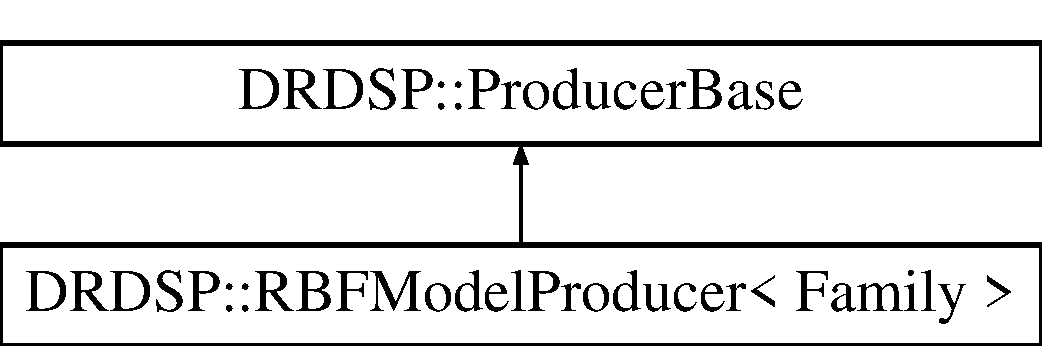
\includegraphics[height=2.000000cm]{struct_d_r_d_s_p_1_1_r_b_f_model_producer}
\end{center}
\end{figure}
\subsection*{Public Types}
\begin{DoxyCompactItemize}
\item 
\hypertarget{struct_d_r_d_s_p_1_1_r_b_f_model_producer_a560d2264a7b87e66d89e34bf0514c9c3}{typedef Family\-::\-Model {\bfseries Model}}\label{struct_d_r_d_s_p_1_1_r_b_f_model_producer_a560d2264a7b87e66d89e34bf0514c9c3}

\end{DoxyCompactItemize}
\subsection*{Public Member Functions}
\begin{DoxyCompactItemize}
\item 
\hypertarget{struct_d_r_d_s_p_1_1_r_b_f_model_producer_abdbffa9162638d17b258fd2af9e867b1}{{\bfseries R\-B\-F\-Model\-Producer} (uint32\-\_\-t num\-R\-B\-Fs)}\label{struct_d_r_d_s_p_1_1_r_b_f_model_producer_abdbffa9162638d17b258fd2af9e867b1}

\item 
\hypertarget{struct_d_r_d_s_p_1_1_r_b_f_model_producer_a16280fd8b2c90a7f1781c36083a8eb8c}{Vector\-Xd {\bfseries Solve} (const \hyperlink{struct_d_r_d_s_p_1_1_family}{Family} \&family, const \hyperlink{struct_d_r_d_s_p_1_1_reduced_data}{Reduced\-Data} \&data) const }\label{struct_d_r_d_s_p_1_1_r_b_f_model_producer_a16280fd8b2c90a7f1781c36083a8eb8c}

\item 
\hypertarget{struct_d_r_d_s_p_1_1_r_b_f_model_producer_aaf6069ba29bae98424669eedaabd33c5}{Model {\bfseries Brute\-Force} (const \hyperlink{struct_d_r_d_s_p_1_1_reduced_data}{Reduced\-Data} \&data, uint32\-\_\-t num\-Iterations) const }\label{struct_d_r_d_s_p_1_1_r_b_f_model_producer_aaf6069ba29bae98424669eedaabd33c5}

\item 
\hypertarget{struct_d_r_d_s_p_1_1_r_b_f_model_producer_ad102d9f22c3052a72989f7725cffe687}{Model {\bfseries Brute\-Force} (const \hyperlink{struct_d_r_d_s_p_1_1_reduced_data}{Reduced\-Data} \&data, uint32\-\_\-t num\-Iterations, uint32\-\_\-t num\-Threads) const }\label{struct_d_r_d_s_p_1_1_r_b_f_model_producer_ad102d9f22c3052a72989f7725cffe687}

\end{DoxyCompactItemize}
\subsection*{Public Attributes}
\begin{DoxyCompactItemize}
\item 
\hypertarget{struct_d_r_d_s_p_1_1_r_b_f_model_producer_aca502a665ad3805c1e879dfa98966414}{double {\bfseries box\-Scale}}\label{struct_d_r_d_s_p_1_1_r_b_f_model_producer_aca502a665ad3805c1e879dfa98966414}

\item 
\hypertarget{struct_d_r_d_s_p_1_1_r_b_f_model_producer_a9734043452d4409fbe078ecad8299b33}{uint32\-\_\-t {\bfseries num\-R\-B\-Fs}}\label{struct_d_r_d_s_p_1_1_r_b_f_model_producer_a9734043452d4409fbe078ecad8299b33}

\end{DoxyCompactItemize}
\subsection*{Protected Member Functions}
\begin{DoxyCompactItemize}
\item 
\hypertarget{struct_d_r_d_s_p_1_1_r_b_f_model_producer_a5f9098538bb68bb948e7f572f6e58a87}{Model {\bfseries Brute\-Force} (const \hyperlink{struct_d_r_d_s_p_1_1_reduced_data}{Reduced\-Data} \&data, const \hyperlink{struct_d_r_d_s_p_1_1_a_a_b_b}{A\-A\-B\-B} \&box, uint32\-\_\-t seed, uint32\-\_\-t num\-Iterations) const }\label{struct_d_r_d_s_p_1_1_r_b_f_model_producer_a5f9098538bb68bb948e7f572f6e58a87}

\end{DoxyCompactItemize}


The documentation for this struct was generated from the following file\-:\begin{DoxyCompactItemize}
\item 
include/\-D\-R\-D\-S\-P/dynamics/rbf\-\_\-model\-\_\-producer.\-h\end{DoxyCompactItemize}

\hypertarget{struct_d_r_d_s_p_1_1_r_b_f_n_l_family}{\section{D\-R\-D\-S\-P\-:\-:R\-B\-F\-N\-L\-Family$<$ F $>$ Struct Template Reference}
\label{struct_d_r_d_s_p_1_1_r_b_f_n_l_family}\index{D\-R\-D\-S\-P\-::\-R\-B\-F\-N\-L\-Family$<$ F $>$@{D\-R\-D\-S\-P\-::\-R\-B\-F\-N\-L\-Family$<$ F $>$}}
}
Inheritance diagram for D\-R\-D\-S\-P\-:\-:R\-B\-F\-N\-L\-Family$<$ F $>$\-:\begin{figure}[H]
\begin{center}
\leavevmode
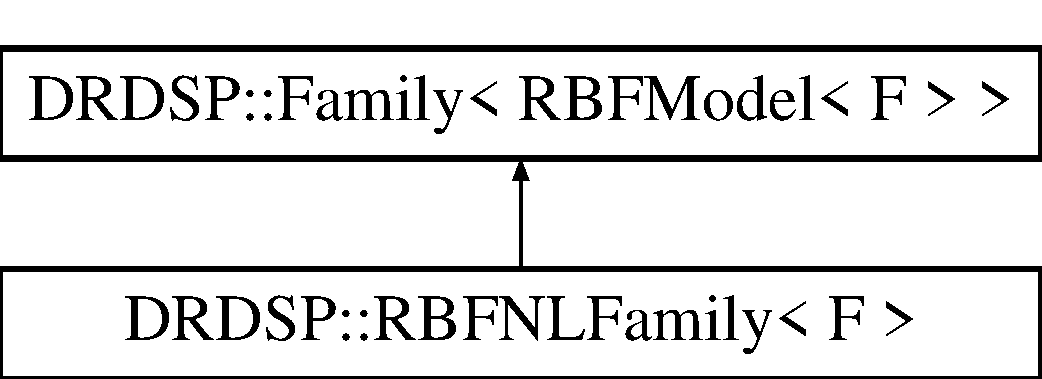
\includegraphics[height=2.000000cm]{struct_d_r_d_s_p_1_1_r_b_f_n_l_family}
\end{center}
\end{figure}
\subsection*{Public Member Functions}
\begin{DoxyCompactItemize}
\item 
\hypertarget{struct_d_r_d_s_p_1_1_r_b_f_n_l_family_a0219576ef1ddd2dc48962f449458f14e}{{\bfseries R\-B\-F\-N\-L\-Family} (uint32\-\_\-t dim, uint32\-\_\-t n\-R\-B\-Fs)}\label{struct_d_r_d_s_p_1_1_r_b_f_n_l_family_a0219576ef1ddd2dc48962f449458f14e}

\item 
\hypertarget{struct_d_r_d_s_p_1_1_r_b_f_n_l_family_ae987ecfe949a27183c7da1440f422cd1}{\hyperlink{struct_d_r_d_s_p_1_1_r_b_f_model}{R\-B\-F\-Model}$<$ F $>$ {\bfseries operator()} (const Vector\-Xd \&parameter) const }\label{struct_d_r_d_s_p_1_1_r_b_f_n_l_family_ae987ecfe949a27183c7da1440f422cd1}

\end{DoxyCompactItemize}
\subsection*{Public Attributes}
\begin{DoxyCompactItemize}
\item 
\hypertarget{struct_d_r_d_s_p_1_1_r_b_f_n_l_family_ac785528e1f2390ad44ed396a4198253d}{uint32\-\_\-t {\bfseries n\-R\-B\-Fs}}\label{struct_d_r_d_s_p_1_1_r_b_f_n_l_family_ac785528e1f2390ad44ed396a4198253d}

\end{DoxyCompactItemize}
\subsection*{Additional Inherited Members}


The documentation for this struct was generated from the following file\-:\begin{DoxyCompactItemize}
\item 
include/\-D\-R\-D\-S\-P/dynamics/rbf\-\_\-family.\-h\end{DoxyCompactItemize}

\hypertarget{struct_d_r_d_s_p_1_1_reduced_data}{\section{D\-R\-D\-S\-P\-:\-:Reduced\-Data Struct Reference}
\label{struct_d_r_d_s_p_1_1_reduced_data}\index{D\-R\-D\-S\-P\-::\-Reduced\-Data@{D\-R\-D\-S\-P\-::\-Reduced\-Data}}
}
\subsection*{Public Member Functions}
\begin{DoxyCompactItemize}
\item 
\hypertarget{struct_d_r_d_s_p_1_1_reduced_data_aaff26858fe467422cfcb125996759ce9}{{\bfseries Reduced\-Data} (uint16\-\_\-t dim, uint32\-\_\-t num\-Points)}\label{struct_d_r_d_s_p_1_1_reduced_data_aaff26858fe467422cfcb125996759ce9}

\item 
\hypertarget{struct_d_r_d_s_p_1_1_reduced_data_a2260037d761f2dc5154c60b4fcba95b3}{{\bfseries Reduced\-Data} (const \hyperlink{struct_d_r_d_s_p_1_1_reduced_data}{Reduced\-Data} \&rhs)}\label{struct_d_r_d_s_p_1_1_reduced_data_a2260037d761f2dc5154c60b4fcba95b3}

\item 
\hypertarget{struct_d_r_d_s_p_1_1_reduced_data_a746ac3e59554e6299e31f79025f4d5f3}{{\bfseries Reduced\-Data} (\hyperlink{struct_d_r_d_s_p_1_1_reduced_data}{Reduced\-Data} \&\&rhs)}\label{struct_d_r_d_s_p_1_1_reduced_data_a746ac3e59554e6299e31f79025f4d5f3}

\item 
\hypertarget{struct_d_r_d_s_p_1_1_reduced_data_a65c05f12dad9db478dd1aaca4486bf3c}{\hyperlink{struct_d_r_d_s_p_1_1_reduced_data}{Reduced\-Data} \& {\bfseries operator=} (const \hyperlink{struct_d_r_d_s_p_1_1_reduced_data}{Reduced\-Data} \&rhs)}\label{struct_d_r_d_s_p_1_1_reduced_data_a65c05f12dad9db478dd1aaca4486bf3c}

\item 
\hypertarget{struct_d_r_d_s_p_1_1_reduced_data_a74732d52875f87cbbbbdb75bb8d51837}{\hyperlink{struct_d_r_d_s_p_1_1_reduced_data}{Reduced\-Data} \& {\bfseries operator=} (\hyperlink{struct_d_r_d_s_p_1_1_reduced_data}{Reduced\-Data} \&\&rhs)}\label{struct_d_r_d_s_p_1_1_reduced_data_a74732d52875f87cbbbbdb75bb8d51837}

\item 
\hypertarget{struct_d_r_d_s_p_1_1_reduced_data_ac53310fd4248f636f24a2041b2df3285}{void {\bfseries Create} (uint16\-\_\-t dim, uint32\-\_\-t num\-Points)}\label{struct_d_r_d_s_p_1_1_reduced_data_ac53310fd4248f636f24a2041b2df3285}

\item 
\hypertarget{struct_d_r_d_s_p_1_1_reduced_data_ae7d05055cf7f171a698dd8bb789cd14d}{void {\bfseries Destroy} ()}\label{struct_d_r_d_s_p_1_1_reduced_data_ae7d05055cf7f171a698dd8bb789cd14d}

\item 
\hypertarget{struct_d_r_d_s_p_1_1_reduced_data_a14c8be432ab0dcd6bf55e22611446440}{void {\bfseries Compute\-Data} (\hyperlink{struct_d_r_d_s_p_1_1_model}{Model} \&model, const \hyperlink{struct_d_r_d_s_p_1_1_data_set}{Data\-Set} \&data, const Matrix\-Xd \&W)}\label{struct_d_r_d_s_p_1_1_reduced_data_a14c8be432ab0dcd6bf55e22611446440}

\item 
\hypertarget{struct_d_r_d_s_p_1_1_reduced_data_a28ffe7941ba57202393ff840a540531f}{void {\bfseries Compute\-Data} (\hyperlink{struct_d_r_d_s_p_1_1_model_c_w}{Model\-C\-W} \&model, const \hyperlink{struct_d_r_d_s_p_1_1_data_set}{Data\-Set} \&data, const Matrix\-Xd \&W)}\label{struct_d_r_d_s_p_1_1_reduced_data_a28ffe7941ba57202393ff840a540531f}

\item 
\hypertarget{struct_d_r_d_s_p_1_1_reduced_data_a49482d08e81e41191b890138f5bfa66e}{void {\bfseries Compute\-Data} (\hyperlink{struct_d_r_d_s_p_1_1_model_parameterized}{Model\-Parameterized} \&model, const Vector\-Xd \&parameter, const \hyperlink{struct_d_r_d_s_p_1_1_data_set}{Data\-Set} \&data, const Matrix\-Xd \&W)}\label{struct_d_r_d_s_p_1_1_reduced_data_a49482d08e81e41191b890138f5bfa66e}

\item 
\hypertarget{struct_d_r_d_s_p_1_1_reduced_data_acea33e5759b6cd9ba56c1b67bb02fb2f}{void {\bfseries Compute\-Data} (\hyperlink{struct_d_r_d_s_p_1_1_model_parameterized_c_w}{Model\-Parameterized\-C\-W} \&model, const Vector\-Xd \&parameter, const \hyperlink{struct_d_r_d_s_p_1_1_data_set}{Data\-Set} \&data, const Matrix\-Xd \&W)}\label{struct_d_r_d_s_p_1_1_reduced_data_acea33e5759b6cd9ba56c1b67bb02fb2f}

\item 
\hypertarget{struct_d_r_d_s_p_1_1_reduced_data_a56bfd420c9dd4e7b9004ef0454fe7abd}{void {\bfseries Compute\-Data} (\hyperlink{struct_d_r_d_s_p_1_1_model_embedded}{Model\-Embedded} \&model, const \hyperlink{struct_d_r_d_s_p_1_1_data_set}{Data\-Set} \&data, const Matrix\-Xd \&W)}\label{struct_d_r_d_s_p_1_1_reduced_data_a56bfd420c9dd4e7b9004ef0454fe7abd}

\item 
\hypertarget{struct_d_r_d_s_p_1_1_reduced_data_a2eb42687ef6683254b9259ce25bfdc00}{void {\bfseries Compute\-Data} (\hyperlink{struct_d_r_d_s_p_1_1_model_parameterized_embedded}{Model\-Parameterized\-Embedded} \&model, const Vector\-Xd \&parameter, const \hyperlink{struct_d_r_d_s_p_1_1_data_set}{Data\-Set} \&data, const Matrix\-Xd \&W)}\label{struct_d_r_d_s_p_1_1_reduced_data_a2eb42687ef6683254b9259ce25bfdc00}

\item 
\hypertarget{struct_d_r_d_s_p_1_1_reduced_data_a13cf0745aa959c739253cd0d19b77d02}{void {\bfseries Compute\-Data} (\hyperlink{struct_d_r_d_s_p_1_1_model_parameterized_embedded_c_w}{Model\-Parameterized\-Embedded\-C\-W} \&model, const Vector\-Xd \&parameter, const \hyperlink{struct_d_r_d_s_p_1_1_data_set}{Data\-Set} \&data, const Matrix\-Xd \&W)}\label{struct_d_r_d_s_p_1_1_reduced_data_a13cf0745aa959c739253cd0d19b77d02}

\item 
\hypertarget{struct_d_r_d_s_p_1_1_reduced_data_ae8d15e5d1a61ed5e495112e4941b9ecb}{\hyperlink{struct_d_r_d_s_p_1_1_a_a_b_b}{A\-A\-B\-B} {\bfseries Compute\-Bounding\-Box} () const }\label{struct_d_r_d_s_p_1_1_reduced_data_ae8d15e5d1a61ed5e495112e4941b9ecb}

\item 
\hypertarget{struct_d_r_d_s_p_1_1_reduced_data_a603dadcceb2b793a76851ec687adad12}{double {\bfseries Compute\-Vector\-Scale} ()}\label{struct_d_r_d_s_p_1_1_reduced_data_a603dadcceb2b793a76851ec687adad12}

\item 
\hypertarget{struct_d_r_d_s_p_1_1_reduced_data_a6b5e802882a81572f3db17e5d1b0afa2}{double {\bfseries Compute\-Derivative\-Scale} ()}\label{struct_d_r_d_s_p_1_1_reduced_data_a6b5e802882a81572f3db17e5d1b0afa2}

\item 
\hypertarget{struct_d_r_d_s_p_1_1_reduced_data_a2eaa9d6f19f0c80998fb06c3f2ef4035}{void {\bfseries Write\-Data} (const char $\ast$filename) const }\label{struct_d_r_d_s_p_1_1_reduced_data_a2eaa9d6f19f0c80998fb06c3f2ef4035}

\item 
\hypertarget{struct_d_r_d_s_p_1_1_reduced_data_a0eedb12f1ca3d0775d10472f491fc72b}{bool {\bfseries Read\-Data} (const char $\ast$filename)}\label{struct_d_r_d_s_p_1_1_reduced_data_a0eedb12f1ca3d0775d10472f491fc72b}

\item 
\hypertarget{struct_d_r_d_s_p_1_1_reduced_data_a79e492ae200fb5da34340f410e158354}{void {\bfseries Write\-Points\-C\-S\-V} (const char $\ast$filename) const }\label{struct_d_r_d_s_p_1_1_reduced_data_a79e492ae200fb5da34340f410e158354}

\item 
\hypertarget{struct_d_r_d_s_p_1_1_reduced_data_a972703812e0d0194e5287966a74df79f}{void {\bfseries Write\-Vectors\-C\-S\-V} (const char $\ast$filename) const }\label{struct_d_r_d_s_p_1_1_reduced_data_a972703812e0d0194e5287966a74df79f}

\end{DoxyCompactItemize}
\subsection*{Public Attributes}
\begin{DoxyCompactItemize}
\item 
\hypertarget{struct_d_r_d_s_p_1_1_reduced_data_a243558842669f45f826d8832931a28da}{Vector\-Xd $\ast$ {\bfseries points}}\label{struct_d_r_d_s_p_1_1_reduced_data_a243558842669f45f826d8832931a28da}

\item 
\hypertarget{struct_d_r_d_s_p_1_1_reduced_data_a07690a84c8d57a4b420e8b889a5d5175}{Vector\-Xd $\ast$ {\bfseries vectors}}\label{struct_d_r_d_s_p_1_1_reduced_data_a07690a84c8d57a4b420e8b889a5d5175}

\item 
\hypertarget{struct_d_r_d_s_p_1_1_reduced_data_a85c036cd52e0d2d6740530f1f4653dff}{Matrix\-Xd $\ast$ {\bfseries derivatives}}\label{struct_d_r_d_s_p_1_1_reduced_data_a85c036cd52e0d2d6740530f1f4653dff}

\item 
\hypertarget{struct_d_r_d_s_p_1_1_reduced_data_ab96e3e52f0f3645ed735c01739b565bb}{double {\bfseries scales} \mbox{[}2\mbox{]}}\label{struct_d_r_d_s_p_1_1_reduced_data_ab96e3e52f0f3645ed735c01739b565bb}

\item 
\hypertarget{struct_d_r_d_s_p_1_1_reduced_data_aed326b4250187f62055aec8fbafc4c45}{uint32\-\_\-t {\bfseries count}}\label{struct_d_r_d_s_p_1_1_reduced_data_aed326b4250187f62055aec8fbafc4c45}

\item 
\hypertarget{struct_d_r_d_s_p_1_1_reduced_data_a15608e335ef89232f565c550262483ba}{uint16\-\_\-t {\bfseries dimension}}\label{struct_d_r_d_s_p_1_1_reduced_data_a15608e335ef89232f565c550262483ba}

\end{DoxyCompactItemize}


The documentation for this struct was generated from the following files\-:\begin{DoxyCompactItemize}
\item 
include/\-D\-R\-D\-S\-P/dynamics/reduced\-\_\-data.\-h\item 
src/dynamics/reduced\-\_\-data.\-cpp\end{DoxyCompactItemize}

\hypertarget{struct_d_r_d_s_p_1_1_reduced_data_system}{\section{D\-R\-D\-S\-P\-:\-:Reduced\-Data\-System Struct Reference}
\label{struct_d_r_d_s_p_1_1_reduced_data_system}\index{D\-R\-D\-S\-P\-::\-Reduced\-Data\-System@{D\-R\-D\-S\-P\-::\-Reduced\-Data\-System}}
}
\subsection*{Public Member Functions}
\begin{DoxyCompactItemize}
\item 
\hypertarget{struct_d_r_d_s_p_1_1_reduced_data_system_a221e3299337151b91fc071ca3f84beb6}{{\bfseries Reduced\-Data\-System} (uint16\-\_\-t N)}\label{struct_d_r_d_s_p_1_1_reduced_data_system_a221e3299337151b91fc071ca3f84beb6}

\item 
\hypertarget{struct_d_r_d_s_p_1_1_reduced_data_system_aea103d77b8ad01f186bbd163a2e432cf}{{\bfseries Reduced\-Data\-System} (const \hyperlink{struct_d_r_d_s_p_1_1_reduced_data_system}{Reduced\-Data\-System} \&rhs)}\label{struct_d_r_d_s_p_1_1_reduced_data_system_aea103d77b8ad01f186bbd163a2e432cf}

\item 
\hypertarget{struct_d_r_d_s_p_1_1_reduced_data_system_adc4e39a9893446b6ad8937bd59bf1b0f}{{\bfseries Reduced\-Data\-System} (\hyperlink{struct_d_r_d_s_p_1_1_reduced_data_system}{Reduced\-Data\-System} \&\&rhs)}\label{struct_d_r_d_s_p_1_1_reduced_data_system_adc4e39a9893446b6ad8937bd59bf1b0f}

\item 
\hypertarget{struct_d_r_d_s_p_1_1_reduced_data_system_af7cd9e3ec1cfadacf761d46fe7f21672}{\hyperlink{struct_d_r_d_s_p_1_1_reduced_data_system}{Reduced\-Data\-System} \& {\bfseries operator=} (const \hyperlink{struct_d_r_d_s_p_1_1_reduced_data_system}{Reduced\-Data\-System} \&rhs)}\label{struct_d_r_d_s_p_1_1_reduced_data_system_af7cd9e3ec1cfadacf761d46fe7f21672}

\item 
\hypertarget{struct_d_r_d_s_p_1_1_reduced_data_system_a91dac8fb109401713b827a327400b164}{\hyperlink{struct_d_r_d_s_p_1_1_reduced_data_system}{Reduced\-Data\-System} \& {\bfseries operator=} (\hyperlink{struct_d_r_d_s_p_1_1_reduced_data_system}{Reduced\-Data\-System} \&\&rhs)}\label{struct_d_r_d_s_p_1_1_reduced_data_system_a91dac8fb109401713b827a327400b164}

\item 
\hypertarget{struct_d_r_d_s_p_1_1_reduced_data_system_a5161bf6e29b60d324025eb56a811217e}{void {\bfseries Create} (uint16\-\_\-t N)}\label{struct_d_r_d_s_p_1_1_reduced_data_system_a5161bf6e29b60d324025eb56a811217e}

\item 
\hypertarget{struct_d_r_d_s_p_1_1_reduced_data_system_ab1eafb140901723d22dc06ca95fb323e}{void {\bfseries Destroy} ()}\label{struct_d_r_d_s_p_1_1_reduced_data_system_ab1eafb140901723d22dc06ca95fb323e}

\item 
\hypertarget{struct_d_r_d_s_p_1_1_reduced_data_system_ae791e9522d7fb6d589c9e1f001eba314}{void {\bfseries Compute\-Data} (\hyperlink{struct_d_r_d_s_p_1_1_model_parameterized}{Model\-Parameterized} \&model, const \hyperlink{struct_d_r_d_s_p_1_1_data_system}{Data\-System} \&data, const Matrix\-Xd \&W)}\label{struct_d_r_d_s_p_1_1_reduced_data_system_ae791e9522d7fb6d589c9e1f001eba314}

\item 
\hypertarget{struct_d_r_d_s_p_1_1_reduced_data_system_a09565a90b382698cd1e24f9bb83c9115}{void {\bfseries Compute\-Data} (\hyperlink{struct_d_r_d_s_p_1_1_model_parameterized_c_w}{Model\-Parameterized\-C\-W} \&model, const \hyperlink{struct_d_r_d_s_p_1_1_data_system}{Data\-System} \&data, const Matrix\-Xd \&W)}\label{struct_d_r_d_s_p_1_1_reduced_data_system_a09565a90b382698cd1e24f9bb83c9115}

\item 
\hypertarget{struct_d_r_d_s_p_1_1_reduced_data_system_ad88bc475b0f2a10539ba5b079c63d28f}{void {\bfseries Compute\-Data} (\hyperlink{struct_d_r_d_s_p_1_1_model_parameterized_embedded}{Model\-Parameterized\-Embedded} \&model, const \hyperlink{struct_d_r_d_s_p_1_1_data_system}{Data\-System} \&data, const Matrix\-Xd \&W)}\label{struct_d_r_d_s_p_1_1_reduced_data_system_ad88bc475b0f2a10539ba5b079c63d28f}

\item 
\hypertarget{struct_d_r_d_s_p_1_1_reduced_data_system_a8a1973de2415d07ac2041b97fbe3e7aa}{void {\bfseries Compute\-Data} (\hyperlink{struct_d_r_d_s_p_1_1_model_parameterized_embedded_c_w}{Model\-Parameterized\-Embedded\-C\-W} \&model, const \hyperlink{struct_d_r_d_s_p_1_1_data_system}{Data\-System} \&data, const Matrix\-Xd \&W)}\label{struct_d_r_d_s_p_1_1_reduced_data_system_a8a1973de2415d07ac2041b97fbe3e7aa}

\item 
\hypertarget{struct_d_r_d_s_p_1_1_reduced_data_system_a21853627f8229be7b5ec278faa31257e}{\hyperlink{struct_d_r_d_s_p_1_1_a_a_b_b}{A\-A\-B\-B} {\bfseries Compute\-Bounding\-Box} () const }\label{struct_d_r_d_s_p_1_1_reduced_data_system_a21853627f8229be7b5ec278faa31257e}

\end{DoxyCompactItemize}
\subsection*{Public Attributes}
\begin{DoxyCompactItemize}
\item 
\hypertarget{struct_d_r_d_s_p_1_1_reduced_data_system_a0a04590789144be3af1cab48ff813c81}{\hyperlink{struct_d_r_d_s_p_1_1_reduced_data}{Reduced\-Data} $\ast$ {\bfseries reduced\-Data}}\label{struct_d_r_d_s_p_1_1_reduced_data_system_a0a04590789144be3af1cab48ff813c81}

\item 
\hypertarget{struct_d_r_d_s_p_1_1_reduced_data_system_a6c869c5a4c0f4346d1c9717ee0667f26}{uint16\-\_\-t {\bfseries num\-Parameters}}\label{struct_d_r_d_s_p_1_1_reduced_data_system_a6c869c5a4c0f4346d1c9717ee0667f26}

\end{DoxyCompactItemize}


The documentation for this struct was generated from the following files\-:\begin{DoxyCompactItemize}
\item 
include/\-D\-R\-D\-S\-P/dynamics/reduced\-\_\-data\-\_\-system.\-h\item 
src/dynamics/reduced\-\_\-data\-\_\-system.\-cpp\end{DoxyCompactItemize}

\hypertarget{struct_d_r_d_s_p_1_1_r_k4}{\section{D\-R\-D\-S\-P\-:\-:R\-K4$<$ F $>$ Struct Template Reference}
\label{struct_d_r_d_s_p_1_1_r_k4}\index{D\-R\-D\-S\-P\-::\-R\-K4$<$ F $>$@{D\-R\-D\-S\-P\-::\-R\-K4$<$ F $>$}}
}
\subsection*{Public Types}
\begin{DoxyCompactItemize}
\item 
\hypertarget{struct_d_r_d_s_p_1_1_r_k4_ade135f12d4119a53c7d7282b0a9de553}{typedef double {\bfseries Time}}\label{struct_d_r_d_s_p_1_1_r_k4_ade135f12d4119a53c7d7282b0a9de553}

\item 
\hypertarget{struct_d_r_d_s_p_1_1_r_k4_a4061ef12d7d212db4d346233710d13f3}{typedef F\-::\-State {\bfseries State}}\label{struct_d_r_d_s_p_1_1_r_k4_a4061ef12d7d212db4d346233710d13f3}

\end{DoxyCompactItemize}
\subsection*{Public Member Functions}
\begin{DoxyCompactItemize}
\item 
\hypertarget{struct_d_r_d_s_p_1_1_r_k4_a7091cac412735b28b5232d2df123e94a}{{\bfseries R\-K4} (const F \&f)}\label{struct_d_r_d_s_p_1_1_r_k4_a7091cac412735b28b5232d2df123e94a}

\item 
\hypertarget{struct_d_r_d_s_p_1_1_r_k4_a16d39b0b28cce9a7cd3e60ba51f36440}{void {\bfseries Integrate} (State \&x, double \&t, double dt)}\label{struct_d_r_d_s_p_1_1_r_k4_a16d39b0b28cce9a7cd3e60ba51f36440}

\item 
\hypertarget{struct_d_r_d_s_p_1_1_r_k4_aba50885ae1bae99d504e1663d0f286f9}{void {\bfseries Integrate} (State \&x, double dt)}\label{struct_d_r_d_s_p_1_1_r_k4_aba50885ae1bae99d504e1663d0f286f9}

\end{DoxyCompactItemize}
\subsection*{Public Attributes}
\begin{DoxyCompactItemize}
\item 
\hypertarget{struct_d_r_d_s_p_1_1_r_k4_af75b6d95493eb7e76dcdcc8bce7946b9}{F {\bfseries f}}\label{struct_d_r_d_s_p_1_1_r_k4_af75b6d95493eb7e76dcdcc8bce7946b9}

\end{DoxyCompactItemize}
\subsection*{Protected Attributes}
\begin{DoxyCompactItemize}
\item 
\hypertarget{struct_d_r_d_s_p_1_1_r_k4_ae9aaed854c424eb85df6a8c175ae034e}{State {\bfseries R\-Kt} \mbox{[}4\mbox{]}}\label{struct_d_r_d_s_p_1_1_r_k4_ae9aaed854c424eb85df6a8c175ae034e}

\end{DoxyCompactItemize}


The documentation for this struct was generated from the following file\-:\begin{DoxyCompactItemize}
\item 
include/\-D\-R\-D\-S\-P/dynamics/rk4.\-h\end{DoxyCompactItemize}

\hypertarget{struct_d_r_d_s_p_1_1_r_k_dynamical_system}{\section{D\-R\-D\-S\-P\-:\-:R\-K\-Dynamical\-System$<$ F, Wrap\-Function $>$ Struct Template Reference}
\label{struct_d_r_d_s_p_1_1_r_k_dynamical_system}\index{D\-R\-D\-S\-P\-::\-R\-K\-Dynamical\-System$<$ F, Wrap\-Function $>$@{D\-R\-D\-S\-P\-::\-R\-K\-Dynamical\-System$<$ F, Wrap\-Function $>$}}
}
Inheritance diagram for D\-R\-D\-S\-P\-:\-:R\-K\-Dynamical\-System$<$ F, Wrap\-Function $>$\-:\begin{figure}[H]
\begin{center}
\leavevmode
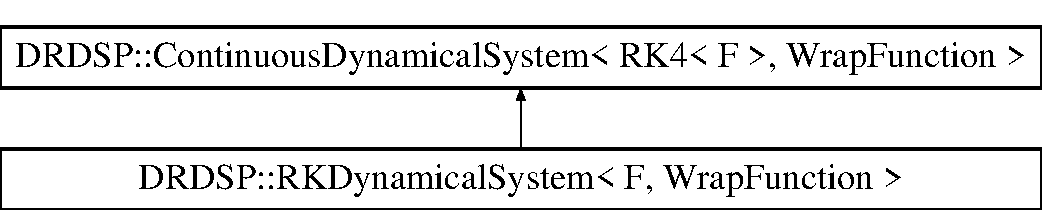
\includegraphics[height=2.000000cm]{struct_d_r_d_s_p_1_1_r_k_dynamical_system}
\end{center}
\end{figure}
\subsection*{Public Member Functions}
\begin{DoxyCompactItemize}
\item 
\hypertarget{struct_d_r_d_s_p_1_1_r_k_dynamical_system_ac4fddbaa65ce84accc167fc446fcfac7}{{\bfseries R\-K\-Dynamical\-System} (const F \&f)}\label{struct_d_r_d_s_p_1_1_r_k_dynamical_system_ac4fddbaa65ce84accc167fc446fcfac7}

\end{DoxyCompactItemize}
\subsection*{Additional Inherited Members}


The documentation for this struct was generated from the following file\-:\begin{DoxyCompactItemize}
\item 
include/\-D\-R\-D\-S\-P/dynamics/dynamical\-System.\-h\end{DoxyCompactItemize}

\hypertarget{struct_eigen_1_1internal_1_1scalar__product__traits_3_01dual_3_01_t_01_4_00_01_t_01_4}{\section{Eigen\-:\-:internal\-:\-:scalar\-\_\-product\-\_\-traits$<$ dual$<$ T $>$, T $>$ Struct Template Reference}
\label{struct_eigen_1_1internal_1_1scalar__product__traits_3_01dual_3_01_t_01_4_00_01_t_01_4}\index{Eigen\-::internal\-::scalar\-\_\-product\-\_\-traits$<$ dual$<$ T $>$, T $>$@{Eigen\-::internal\-::scalar\-\_\-product\-\_\-traits$<$ dual$<$ T $>$, T $>$}}
}
\subsection*{Public Types}
\begin{DoxyCompactItemize}
\item 
enum \{ {\bfseries Defined} = 1
 \}
\item 
\hypertarget{struct_eigen_1_1internal_1_1scalar__product__traits_3_01dual_3_01_t_01_4_00_01_t_01_4_a0a57bae15d94b88ccb84644c4a52fcdf}{typedef \hyperlink{struct_d_r_d_s_p_1_1dual}{dual}$<$ T $>$ {\bfseries Return\-Type}}\label{struct_eigen_1_1internal_1_1scalar__product__traits_3_01dual_3_01_t_01_4_00_01_t_01_4_a0a57bae15d94b88ccb84644c4a52fcdf}

\end{DoxyCompactItemize}


The documentation for this struct was generated from the following file\-:\begin{DoxyCompactItemize}
\item 
include/\-D\-R\-D\-S\-P/eigen\-\_\-dual.\-h\end{DoxyCompactItemize}

\hypertarget{struct_eigen_1_1internal_1_1scalar__product__traits_3_01_t_00_01dual_3_01_t_01_4_01_4}{\section{Eigen\-:\-:internal\-:\-:scalar\-\_\-product\-\_\-traits$<$ T, dual$<$ T $>$ $>$ Struct Template Reference}
\label{struct_eigen_1_1internal_1_1scalar__product__traits_3_01_t_00_01dual_3_01_t_01_4_01_4}\index{Eigen\-::internal\-::scalar\-\_\-product\-\_\-traits$<$ T, dual$<$ T $>$ $>$@{Eigen\-::internal\-::scalar\-\_\-product\-\_\-traits$<$ T, dual$<$ T $>$ $>$}}
}
\subsection*{Public Types}
\begin{DoxyCompactItemize}
\item 
enum \{ {\bfseries Defined} = 1
 \}
\item 
\hypertarget{struct_eigen_1_1internal_1_1scalar__product__traits_3_01_t_00_01dual_3_01_t_01_4_01_4_ade2ec61ed4cbf4c325f0eb3f80a31918}{typedef \hyperlink{struct_d_r_d_s_p_1_1dual}{dual}$<$ T $>$ {\bfseries Return\-Type}}\label{struct_eigen_1_1internal_1_1scalar__product__traits_3_01_t_00_01dual_3_01_t_01_4_01_4_ade2ec61ed4cbf4c325f0eb3f80a31918}

\end{DoxyCompactItemize}


The documentation for this struct was generated from the following file\-:\begin{DoxyCompactItemize}
\item 
include/\-D\-R\-D\-S\-P/eigen\-\_\-dual.\-h\end{DoxyCompactItemize}

\hypertarget{struct_d_r_d_s_p_1_1_secant_cost_function}{\section{D\-R\-D\-S\-P\-:\-:Secant\-Cost\-Function Struct Reference}
\label{struct_d_r_d_s_p_1_1_secant_cost_function}\index{D\-R\-D\-S\-P\-::\-Secant\-Cost\-Function@{D\-R\-D\-S\-P\-::\-Secant\-Cost\-Function}}
}
\subsection*{Public Member Functions}
\begin{DoxyCompactItemize}
\item 
\hypertarget{struct_d_r_d_s_p_1_1_secant_cost_function_a5c2b61c470824d3fe68b3a089167d183}{{\bfseries Secant\-Cost\-Function} (const \hyperlink{struct_d_r_d_s_p_1_1_secants_pre_computed}{Secants\-Pre\-Computed} \&secants)}\label{struct_d_r_d_s_p_1_1_secant_cost_function_a5c2b61c470824d3fe68b3a089167d183}

\item 
\hypertarget{struct_d_r_d_s_p_1_1_secant_cost_function_ad30d19180f9c1e9dac7f9ae87296a0f8}{double {\bfseries operator()} (const Matrix\-Xd \&X) const }\label{struct_d_r_d_s_p_1_1_secant_cost_function_ad30d19180f9c1e9dac7f9ae87296a0f8}

\end{DoxyCompactItemize}
\subsection*{Public Attributes}
\begin{DoxyCompactItemize}
\item 
\hypertarget{struct_d_r_d_s_p_1_1_secant_cost_function_aa020a6fb9605b1e4f1e21a343186bd74}{const \hyperlink{struct_d_r_d_s_p_1_1_secants_pre_computed}{Secants\-Pre\-Computed} \& {\bfseries secants}}\label{struct_d_r_d_s_p_1_1_secant_cost_function_aa020a6fb9605b1e4f1e21a343186bd74}

\end{DoxyCompactItemize}


The documentation for this struct was generated from the following files\-:\begin{DoxyCompactItemize}
\item 
include/\-D\-R\-D\-S\-P/projection/proj\-\_\-secant.\-h\item 
src/projection/proj\-\_\-secant.\-cpp\end{DoxyCompactItemize}

\hypertarget{struct_d_r_d_s_p_1_1_secant_cost_function_multi}{\section{D\-R\-D\-S\-P\-:\-:Secant\-Cost\-Function\-Multi Struct Reference}
\label{struct_d_r_d_s_p_1_1_secant_cost_function_multi}\index{D\-R\-D\-S\-P\-::\-Secant\-Cost\-Function\-Multi@{D\-R\-D\-S\-P\-::\-Secant\-Cost\-Function\-Multi}}
}
\subsection*{Public Member Functions}
\begin{DoxyCompactItemize}
\item 
\hypertarget{struct_d_r_d_s_p_1_1_secant_cost_function_multi_a4408a82da556da38e458fc2565c49891}{{\bfseries Secant\-Cost\-Function\-Multi} (const \hyperlink{struct_d_r_d_s_p_1_1_secants}{Secants} $\ast$secants, size\-\_\-t N)}\label{struct_d_r_d_s_p_1_1_secant_cost_function_multi_a4408a82da556da38e458fc2565c49891}

\item 
\hypertarget{struct_d_r_d_s_p_1_1_secant_cost_function_multi_a40271ed4db634786ff8732acb99e7ddb}{double {\bfseries operator()} (const Matrix\-Xd \&X) const }\label{struct_d_r_d_s_p_1_1_secant_cost_function_multi_a40271ed4db634786ff8732acb99e7ddb}

\end{DoxyCompactItemize}
\subsection*{Public Attributes}
\begin{DoxyCompactItemize}
\item 
\hypertarget{struct_d_r_d_s_p_1_1_secant_cost_function_multi_a5433e39d7091e942a4d9e09bbc74871f}{const \hyperlink{struct_d_r_d_s_p_1_1_secants}{Secants} $\ast$ {\bfseries secants}}\label{struct_d_r_d_s_p_1_1_secant_cost_function_multi_a5433e39d7091e942a4d9e09bbc74871f}

\item 
\hypertarget{struct_d_r_d_s_p_1_1_secant_cost_function_multi_a7c2b1b7e3474de697285d9265ed60c39}{size\-\_\-t {\bfseries N}}\label{struct_d_r_d_s_p_1_1_secant_cost_function_multi_a7c2b1b7e3474de697285d9265ed60c39}

\end{DoxyCompactItemize}


The documentation for this struct was generated from the following files\-:\begin{DoxyCompactItemize}
\item 
include/\-D\-R\-D\-S\-P/projection/proj\-\_\-secant.\-h\item 
src/projection/proj\-\_\-secant.\-cpp\end{DoxyCompactItemize}

\hypertarget{struct_d_r_d_s_p_1_1_secant_cost_gradient}{\section{D\-R\-D\-S\-P\-:\-:Secant\-Cost\-Gradient Struct Reference}
\label{struct_d_r_d_s_p_1_1_secant_cost_gradient}\index{D\-R\-D\-S\-P\-::\-Secant\-Cost\-Gradient@{D\-R\-D\-S\-P\-::\-Secant\-Cost\-Gradient}}
}
\subsection*{Public Member Functions}
\begin{DoxyCompactItemize}
\item 
\hypertarget{struct_d_r_d_s_p_1_1_secant_cost_gradient_a2587363d1bfdf4b981276b18bfae1936}{{\bfseries Secant\-Cost\-Gradient} (const \hyperlink{struct_d_r_d_s_p_1_1_secants}{Secants} \&secants)}\label{struct_d_r_d_s_p_1_1_secant_cost_gradient_a2587363d1bfdf4b981276b18bfae1936}

\item 
\hypertarget{struct_d_r_d_s_p_1_1_secant_cost_gradient_a2323e393882ab1cd60fb1bb61b587a92}{Matrix\-Xd {\bfseries operator()} (const Matrix\-Xd \&X) const }\label{struct_d_r_d_s_p_1_1_secant_cost_gradient_a2323e393882ab1cd60fb1bb61b587a92}

\item 
\hypertarget{struct_d_r_d_s_p_1_1_secant_cost_gradient_a0cb0bc11cc41452cde8eb15c623c8ea5}{\hyperlink{struct_d_r_d_s_p_1_1_secant_cost_gradient}{Secant\-Cost\-Gradient} \& {\bfseries operator=} (const \hyperlink{struct_d_r_d_s_p_1_1_secant_cost_gradient}{Secant\-Cost\-Gradient} \&)=delete}\label{struct_d_r_d_s_p_1_1_secant_cost_gradient_a0cb0bc11cc41452cde8eb15c623c8ea5}

\end{DoxyCompactItemize}
\subsection*{Public Attributes}
\begin{DoxyCompactItemize}
\item 
\hypertarget{struct_d_r_d_s_p_1_1_secant_cost_gradient_a8620cf3251ef7fc475cd713b74ad3770}{const \hyperlink{struct_d_r_d_s_p_1_1_secants}{Secants} \& {\bfseries secants}}\label{struct_d_r_d_s_p_1_1_secant_cost_gradient_a8620cf3251ef7fc475cd713b74ad3770}

\end{DoxyCompactItemize}


The documentation for this struct was generated from the following files\-:\begin{DoxyCompactItemize}
\item 
include/\-D\-R\-D\-S\-P/projection/proj\-\_\-secant.\-h\item 
src/projection/proj\-\_\-secant.\-cpp\end{DoxyCompactItemize}

\hypertarget{struct_d_r_d_s_p_1_1_secant_cost_gradient_multi}{\section{D\-R\-D\-S\-P\-:\-:Secant\-Cost\-Gradient\-Multi Struct Reference}
\label{struct_d_r_d_s_p_1_1_secant_cost_gradient_multi}\index{D\-R\-D\-S\-P\-::\-Secant\-Cost\-Gradient\-Multi@{D\-R\-D\-S\-P\-::\-Secant\-Cost\-Gradient\-Multi}}
}
\subsection*{Public Member Functions}
\begin{DoxyCompactItemize}
\item 
\hypertarget{struct_d_r_d_s_p_1_1_secant_cost_gradient_multi_a4ca34beff67912da82ee2c38c3067b70}{{\bfseries Secant\-Cost\-Gradient\-Multi} (const \hyperlink{struct_d_r_d_s_p_1_1_secants}{Secants} $\ast$secants, size\-\_\-t N)}\label{struct_d_r_d_s_p_1_1_secant_cost_gradient_multi_a4ca34beff67912da82ee2c38c3067b70}

\item 
\hypertarget{struct_d_r_d_s_p_1_1_secant_cost_gradient_multi_ac5d9872ad2ea3cfaa093701147eb9e59}{Matrix\-Xd {\bfseries operator()} (const Matrix\-Xd \&X) const }\label{struct_d_r_d_s_p_1_1_secant_cost_gradient_multi_ac5d9872ad2ea3cfaa093701147eb9e59}

\end{DoxyCompactItemize}
\subsection*{Public Attributes}
\begin{DoxyCompactItemize}
\item 
\hypertarget{struct_d_r_d_s_p_1_1_secant_cost_gradient_multi_a2725c1b2c8c4ff707df7b9d62524a09e}{const \hyperlink{struct_d_r_d_s_p_1_1_secants}{Secants} $\ast$ {\bfseries secants}}\label{struct_d_r_d_s_p_1_1_secant_cost_gradient_multi_a2725c1b2c8c4ff707df7b9d62524a09e}

\item 
\hypertarget{struct_d_r_d_s_p_1_1_secant_cost_gradient_multi_a44b55a4bb3da9af972fa093a77e83662}{size\-\_\-t {\bfseries N}}\label{struct_d_r_d_s_p_1_1_secant_cost_gradient_multi_a44b55a4bb3da9af972fa093a77e83662}

\end{DoxyCompactItemize}


The documentation for this struct was generated from the following files\-:\begin{DoxyCompactItemize}
\item 
include/\-D\-R\-D\-S\-P/projection/proj\-\_\-secant.\-h\item 
src/projection/proj\-\_\-secant.\-cpp\end{DoxyCompactItemize}

\hypertarget{struct_d_r_d_s_p_1_1_secants}{\section{D\-R\-D\-S\-P\-:\-:Secants Struct Reference}
\label{struct_d_r_d_s_p_1_1_secants}\index{D\-R\-D\-S\-P\-::\-Secants@{D\-R\-D\-S\-P\-::\-Secants}}
}


Base class/interface for a set of secants.  




{\ttfamily \#include $<$secants.\-h$>$}

Inheritance diagram for D\-R\-D\-S\-P\-:\-:Secants\-:\begin{figure}[H]
\begin{center}
\leavevmode
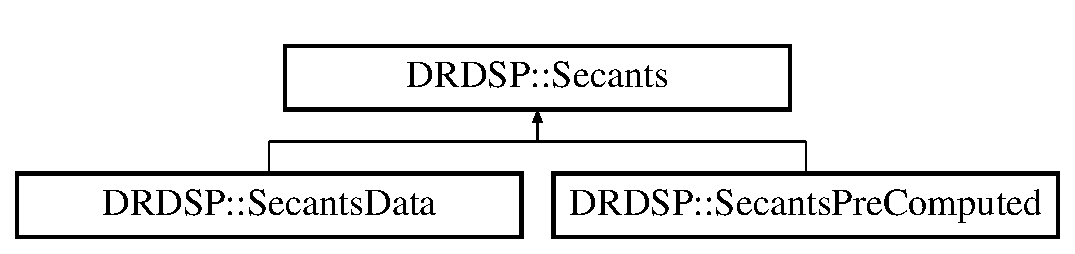
\includegraphics[height=2.000000cm]{struct_d_r_d_s_p_1_1_secants}
\end{center}
\end{figure}
\subsection*{Public Member Functions}
\begin{DoxyCompactItemize}
\item 
\hypertarget{struct_d_r_d_s_p_1_1_secants_aa36f3ff75b75d498e585cbac447cede9}{virtual Vector\-Xd \hyperlink{struct_d_r_d_s_p_1_1_secants_aa36f3ff75b75d498e585cbac447cede9}{Get\-Secant} (size\-\_\-t k) const =0}\label{struct_d_r_d_s_p_1_1_secants_aa36f3ff75b75d498e585cbac447cede9}

\begin{DoxyCompactList}\small\item\em Get the kth secant (normalized) \end{DoxyCompactList}\item 
\hypertarget{struct_d_r_d_s_p_1_1_secants_a96e9a725643c31456df79a797f427981}{virtual Vector\-Xd \hyperlink{struct_d_r_d_s_p_1_1_secants_a96e9a725643c31456df79a797f427981}{Get\-Secant\-No\-Normalize} (size\-\_\-t k) const =0}\label{struct_d_r_d_s_p_1_1_secants_a96e9a725643c31456df79a797f427981}

\begin{DoxyCompactList}\small\item\em Get the kth secant (not necessarily normalized) \end{DoxyCompactList}\item 
\hypertarget{struct_d_r_d_s_p_1_1_secants_a9b6763bc1541a775e842e437448200ef}{virtual \hyperlink{struct_d_r_d_s_p_1_1_secants_pre_computed}{Secants\-Pre\-Computed} {\bfseries Cull\-Secants} (double tolerance) const }\label{struct_d_r_d_s_p_1_1_secants_a9b6763bc1541a775e842e437448200ef}

\item 
\hypertarget{struct_d_r_d_s_p_1_1_secants_abc02bf01e73c2d89848a090c88666291}{\hyperlink{struct_d_r_d_s_p_1_1_secants_pre_computed}{Secants\-Pre\-Computed} {\bfseries Cull\-Secants\-Degrees} (double degrees) const }\label{struct_d_r_d_s_p_1_1_secants_abc02bf01e73c2d89848a090c88666291}

\item 
\hypertarget{struct_d_r_d_s_p_1_1_secants_aec22fc746a9047366d7b81729a2e4f8a}{\hyperlink{struct_d_r_d_s_p_1_1_secants_pre_computed}{Secants\-Pre\-Computed} {\bfseries Cull\-Secants\-Radians} (double radians) const }\label{struct_d_r_d_s_p_1_1_secants_aec22fc746a9047366d7b81729a2e4f8a}

\end{DoxyCompactItemize}
\subsection*{Public Attributes}
\begin{DoxyCompactItemize}
\item 
\hypertarget{struct_d_r_d_s_p_1_1_secants_a821f5d19109ca4f94a7fb593614ac173}{size\-\_\-t \hyperlink{struct_d_r_d_s_p_1_1_secants_a821f5d19109ca4f94a7fb593614ac173}{count}}\label{struct_d_r_d_s_p_1_1_secants_a821f5d19109ca4f94a7fb593614ac173}

\begin{DoxyCompactList}\small\item\em Number of secants in the data set. \end{DoxyCompactList}\item 
\hypertarget{struct_d_r_d_s_p_1_1_secants_a950d625f7d298f93eaad20062f79db1b}{uint32\-\_\-t \hyperlink{struct_d_r_d_s_p_1_1_secants_a950d625f7d298f93eaad20062f79db1b}{dimension}}\label{struct_d_r_d_s_p_1_1_secants_a950d625f7d298f93eaad20062f79db1b}

\begin{DoxyCompactList}\small\item\em Dimension of the space. \end{DoxyCompactList}\end{DoxyCompactItemize}


\subsection{Detailed Description}
Base class/interface for a set of secants. 

The documentation for this struct was generated from the following files\-:\begin{DoxyCompactItemize}
\item 
include/\-D\-R\-D\-S\-P/data/secants.\-h\item 
src/data/secants.\-cpp\end{DoxyCompactItemize}

\hypertarget{struct_d_r_d_s_p_1_1_traits}{\section{D\-R\-D\-S\-P\-:\-:Traits$<$ V $>$ Struct Template Reference}
\label{struct_d_r_d_s_p_1_1_traits}\index{D\-R\-D\-S\-P\-::\-Traits$<$ V $>$@{D\-R\-D\-S\-P\-::\-Traits$<$ V $>$}}
}


The documentation for this struct was generated from the following file\-:\begin{DoxyCompactItemize}
\item 
include/\-D\-R\-D\-S\-P/geometry/geodesic.\-h\end{DoxyCompactItemize}

\hypertarget{struct_d_r_d_s_p_1_1_uniform_metric}{\section{D\-R\-D\-S\-P\-:\-:Uniform\-Metric$<$ Point, Inner\-Product $>$ Struct Template Reference}
\label{struct_d_r_d_s_p_1_1_uniform_metric}\index{D\-R\-D\-S\-P\-::\-Uniform\-Metric$<$ Point, Inner\-Product $>$@{D\-R\-D\-S\-P\-::\-Uniform\-Metric$<$ Point, Inner\-Product $>$}}
}
\subsection*{Public Types}
\begin{DoxyCompactItemize}
\item 
\hypertarget{struct_d_r_d_s_p_1_1_uniform_metric_ac3dcdc4791e2c355540524ac3eb88b58}{typedef Point {\bfseries Point}}\label{struct_d_r_d_s_p_1_1_uniform_metric_ac3dcdc4791e2c355540524ac3eb88b58}

\item 
\hypertarget{struct_d_r_d_s_p_1_1_uniform_metric_a4f7e6f085e48e4496bb8747368e4e4aa}{typedef Inner\-Product {\bfseries Inner\-Product}}\label{struct_d_r_d_s_p_1_1_uniform_metric_a4f7e6f085e48e4496bb8747368e4e4aa}

\end{DoxyCompactItemize}
\subsection*{Public Member Functions}
\begin{DoxyCompactItemize}
\item 
\hypertarget{struct_d_r_d_s_p_1_1_uniform_metric_a731c6750b68fd705e740b620a72a8f9f}{Inner\-Product {\bfseries operator()} (const Point \&) const }\label{struct_d_r_d_s_p_1_1_uniform_metric_a731c6750b68fd705e740b620a72a8f9f}

\end{DoxyCompactItemize}


The documentation for this struct was generated from the following file\-:\begin{DoxyCompactItemize}
\item 
include/\-D\-R\-D\-S\-P/geometry/metric.\-h\end{DoxyCompactItemize}

%--- End generated contents ---

% Index
\newpage
\phantomsection
\addcontentsline{toc}{part}{Index}
\printindex

\end{document}
